\documentclass[a4paper,11pt]{report}
\usepackage[left=4.0cm,right=2.0cm,vmargin=2.0cm]{geometry}

\usepackage{MinionPro}

\usepackage[utf8x]{inputenc}
\PrerenderUnicode{ä}
\PrerenderUnicode{ü}
\PrerenderUnicode{ö}

\usepackage{url}
\usepackage{graphicx}
\usepackage[vlined]{algorithm2e}
\usepackage{listings,color}
\usepackage{amsthm}
\usepackage[hang,flushmargin]{footmisc}
\usepackage{xspace}
\usepackage[pdftex, bookmarks=true, bookmarksnumbered=true, bookmarksopenlevel=0,hyperfootnotes=false,bookmarksopen=true]{hyperref}
\usepackage{multicol}
\usepackage{setspace}

\pdfadjustspacing=1
\parindent = 0.0cm
\parskip = 0.2cm
\setlength{\parskip}{0.3cm plus 0.2cm minus 0.2cm}
\clubpenalty = 300
\widowpenalty = 300
\hyphenpenalty = 0
\displaywidowpenalty = 10000
\onehalfspacing

\definecolor{_orange}{rgb}{0.97,0.5,0.04}
\definecolor{_gray}{rgb}{0.35,0.35,0.35}
\definecolor{_lightgray}{rgb}{0.93,0.93,0.93}
\definecolor{_blue}{rgb}{0.14, 0.43, 0.69}

\lstdefinelanguage{Sage}[]{Python}
{morekeywords={True,False,sage,with},
sensitive=true}

\lstset{frame=none,
          showtabs=False,
          showspaces=False,
          showstringspaces=False,
          keywordstyle={\bf },
          language = Sage,
          basicstyle=\small\ttfamily\singlespacing
          }

\hypersetup{
 pdfauthor = {Martin Albrecht},
 pdftitle = {PhD Thesis},
 colorlinks = true,
 linkcolor = black,
 citecolor = black,
 urlcolor = black,
}

\title{Algorithmic Algebraic Techniques and their Application to Block Cipher Cryptanalysis}
\author{Martin Albrecht\\M.R.Albrecht@rhul.ac.uk}

% Systems
\newcommand{\Sage}{Sage\xspace}
\newcommand{\Singular}{\textsc{Singular}\xspace}
\newcommand{\PolyBoRi}{\textsc{PolyBoRi}\xspace}
\newcommand{\Magma}{\textsc{Magma}\xspace}
\newcommand{\GAP}{GAP\xspace}
\newcommand{\MiniSat}{\textsc{MiniSat}\xspace}
\newcommand{\CryptoMiniSat}{\textsc{Crypto\-Mini\-Sat}\xspace}

% CPUs
\newcommand{\xBG}{\textsf{x86\_64}\xspace}
\newcommand{\Opteron}{\textsf{Opteron}\xspace}
\newcommand{\CTD}{\textsf{Core 2 Duo}\xspace}
\newcommand{\CT}{\textsf{Core 2}\xspace}
\newcommand{\Xeon}{\textsf{Xeon}\xspace}

% Ciphers
\newcommand{\PRESENT}{\textsc{Present}\xspace}

% Fields
\newcommand{\field}[1]{\ensuremath{\mathbb{#1}}\xspace}
\newcommand{\F}{\ensuremath{\field{F}}\xspace}
\newcommand{\Z}{\field{Z}}
\newcommand{\e}{\ensuremath{\mathbf{e}}\xspace}
\newcommand{\N}{\field{N}}
\newcommand{\GFZ}{\ensuremath{\field{F}_2}\xspace}
\renewcommand{\mod}{\ \%\ }

% Commutative Algebra
\newcommand{\ideal}[1]{\langle {#1} \rangle}
\newcommand{\Mac}[1]{\ensuremath{\mathcal{M}^{acaulay}_{#1}}}
\newcommand{\LCM}{\ensuremath{\textsc{LCM}}\xspace}
\newcommand{\LM}{\ensuremath{\textsc{LM}}\xspace}
\newcommand{\LC}{\ensuremath{\textsc{LC}}\xspace}
\newcommand{\LT}{\ensuremath{\textsc{LT}}\xspace}

\newcommand{\sig}{\ensuremath{\textnormal{sig}}}
\newcommand{\idx}{\ensuremath{\textnormal{idx}}}
\newcommand{\poly}{\ensuremath{\textnormal{poly}}}
\newcommand{\expvec}{\ensuremath{\textnormal{expvec}}}
\newcommand{\pring}{\ensuremath{\mathcal{R}}}
\newcommand{\sigset}{\ensuremath{\mathcal{S}}}


\newcommand{\ord}[1]{\ensuremath{\mathcal{O}\!\left(#1\right)}}


\newtheorem{theorem}{Theorem}[section]
\newtheorem{corollary}[theorem]{Corollary}
\newtheorem{lemma}[theorem]{Lemma}
\newtheorem{proposition}[theorem]{Proposition}
\newtheorem{notation}[theorem]{Notation}

\newtheorem{example}{Example}[section]
\newtheorem{definition}{Definition}[section]

\newenvironment{citeproof}{\vspace{0.3cm}\emph{Proof.}}{\vspace{0.3cm}}
\newcommand{\needcite}{\textbf{citation needed!}\xspace}

\theoremstyle{definition}
\newtheorem{alg}{Algorithm}

\date{\vspace{8cm}Thesis submitted to\\Royal Holloway, University of London\\ for the degree of\\Doctor of Philosophy 2010.}
\begin{document}

\maketitle


\newpage

\addtocounter{page}{1}

\chapter*{Declaration}
\thispagestyle{empty}
These doctoral studies were conducted under the supervision of Dr.\ Carlos Cid.

The work presented in this thesis is the result of original research carried out by myself, in collaboration with others, whilst enrolled in the Department of Mathematics as a candidate for the degree of Doctor of Philosophy. This work has not been submitted for any other degree or award in any other university or educational establishment.

Some of the work presented in this thesis was previously published in the following works:
\begin{itemize}
 \item Martin Albrecht. Algebraic attacks on the Courtois Toy Cipher. \emph{Cryptologia}, 32:220–276, 2008.
 \item Martin Albrecht, Gregory V.\ Bard, and William Hart. Algorithm 898: Efficient multiplication of dense matrices over GF(2). \emph{ACM Transactions on Mathematical Software}, 37(1), 2009.
 \item Martin Albrecht and Carlos Cid. Algebraic Techniques in Differential Cryptanalysis. \emph{Fast Software Encryption 2009}, Lecture Notes in Computer Science, Berlin, Heidelberg, New York, 2009. Springer Verlag.
\item Martin Albrecht and Carlos Cid. Cold Boot Key Recovery using Polynomial System Solving with Noise presented at \emph{2nd International Conference on Symbolic Computation and Cryptography}, Egham, UK. 2010.
\item Martin Albrecht, Carlos Cid, Thomas Dullien, Jean-Charles Faugère and Ludovic Perret. Algebraic Precomputations in Differential and Integral Cryptanalysis. \emph{6th China International Conference on Information Security and Cryptology}, 2010.
\item Martin Albrecht and Clément Pernet. Efficient Decomposition of Dense Matrices over GF(2) presented at the ECrypt \emph{Tools for Cryptanalysis 2010} workshop, Egham, UK. 2010.
\end{itemize}

In all works all authors contributed equally. All experiments presented in this thesis and the works listed above were conducted by the author.

\vspace{2cm}

\begin{flushright}
Martin Albrecht\\
July 2010
\end{flushright}

\chapter*{Abstract}
In Part~\ref{part:la} we present and discuss implementations of both well-known and novel algorithms for fundamental problems of linear algebra over the field with two elements (\GFZ). In particular, we present the best known implementations for matrix-matrix multiplication and matrix decomposition for dense matrices over \GFZ. These implementations are based on novel variants of the ``M4RM'' multiplication algorithm and the M4RI elimination algorithm.

In Part~\ref{part:gb} we discuss Gröbner basis algorithms. No algorithm discussed in this part is new. However, we are not aware of any other treatment of either the matrix-$F_5$ or the $F_4$-style $F_5$ in the English speaking literature which covers these algorithms in such detail. Furthermore, we provide reference implementations for all algorithms discussed in this part. 
In Part~\ref{part:ac} we apply algebraic techniques to the cryptanalysis of block ciphers. The key contributions of this part are novel ways of utilising algebraic techniques in cryptanalysis. In particular, we combine algebraic techniques with linear, differential and higher-order differential cryptanalysis. These hybrid approaches allow us to push the respective cryptanalytical technique further in most cases. We also explicitly shift the focus from solving polynomial systems of equations to computing features about block ciphers which can then be used in other attacks. Finally, we propose a new family of problems -- denoted ``Max-PoSSo'' in this thesis -- which model polynomial system solving with noise. We also propose an algorithm for solving these problems, based on Integer Programming, and apply this algorithm to the so-called ``Cold Boot'' problem.

\chapter*{Foreword}
We are standing on the shoulders of giants, so far so general. However, the relative novelty of the fields of cryptography and computational mathematics and the large number conferences, workshops and research links in these areas allow us to meet some of these giants in our fields. In the past three years I had the pleasure of meeting many top researchers in my fields and was also given the opportunity to discuss my often naive problems with them. For this, I am deeply grateful. Not only because these researchers patiently corrected my many mistakes but also because the ECrypt~2 EU project and the Information Security Group funded, supported and thus made possible my travels to workshops, conferences, meetings and other departments. I doubt my research would have turned out the way it did without these lively contacts with the wider research community. 

In a similar fashion the Sage mathematics software project should be mentioned. This project, under the guidance of William Stein, exposed me to a much wider research community than I would have engaged with otherwise. Especially the first part of this thesis is witness to the productive collaborations which arose from this exposure. However, the Sage signature can be found in any given chapter of this thesis. It is not only the direct production of research papers that I took from the Sage project. Without this flexible environment many experiments conducted in this thesis -- which are exclusively performed using Sage -- would have taking much longer and possibly some insights would have been missed. This also applies to the generous support given by William Stein and the Information Security Group in the form of computer resources\footnote{William Stein's computer was purchased under National Science Foundation Grant No. DMS-0821725.}. William Stein and the Sage project also inspired through example: in this project high school students write and review code and documentation alongside distinguished professors as equals. The spirit of the Sage community, especially during the first few Sage workshops, had a severe impact on myself as a researcher.

On a quite fundamental level this thesis would not have been possible without the Royal Holloway Valerie Myerscough Scholarship which funded my studies.

I am deeply grateful to my PhD supervisor Carlos Cid for this supervision, advice and key scientific insights guiding me to the completion of this thesis. Whenever I lost track on how to proceed he offered helpful advice. On the other hand, he encouraged me to pursue my own side-projects allowing me to expand my horizon. Carlos also made numerous suggestions on how to improve this thesis and without his input many issues would not have been spotted. All remaining errors are of course my own. I was lucky to have Carlos Cid as my supervisor. I also wish to thank my PhD adviser Kenneth Paterson with whom I collaborated on several occasions during my PhD. He was key in exposing and pushing me to areas of cryptographic research outside of the topics covered in this thesis. To both researchers I am also grateful for giving advice on more general research questions, career decisions and their general support. I also wish to thank Michael Hortmann who supervised my Diplomarbeit on algebraic attacks which was my entry to cryptographic research.

It is only now that I fully realise how much support I have received from my parents over the past decades which allowed me to pursue this research career path. Their strong appreciation for science, enlightenment and knowledge, their fostering of my interests in computers at a young age and their continued support not only during these past three years made this thesis possible.

Many people provided feedback on individual chapters of this thesis or papers on which some of these chapters are based. These are Gregory Bard, Robert Bradshaw, Michael Brickenstein, Tom Boothby, Stanislav Bulygin, Carlos Cid, Thomas Dullien, Christian Eder, Pooya Farshim, Jean-Charles Faugère, William Hart, Georg Lippold, Wael Said Abd Elmageed Mohamed, Sean Murphy, Matt Robshaw, Cl{\'e}ment Pernet, Ludovic Perret, John Perry, Allan Steel and Ralf-Phillip Weinmann. Since some of the chapters in this thesis are revised versions of published articles anonymous referees also provided feedback and helpful discussions. Furthermore, I wish to express my gratitude towards my co-authors from papers which are not included in this thesis and who were not mentioned so far, these are in alphabetic order: Craig Gentry, Shai Halevi, Jonathan Katz and Gaven Watson.

I finish by expressing my gratitude and appreciation to the one person who probably influenced this thesis the most despite not taking a particular strong interest in my research: Silke Jahn. I cannot think of anyone whose opinion I value more.

\begin{flushright}
-- Martin Albrecht
\end{flushright}


\newpage

\setcounter{tocdepth}{1}
\tableofcontents


\part{Linear Algebra}
\label{part:la}

\chapter{Efficient Multiplication of Dense Matrices over GF(2)}
\label{chapter:matmul}
This chapter is a revised and updated version of the paper ``Algorithm 898: Efficient Multiplication of Dense Matrices over GF(2)'' by the author, Gregory Bard and William Hart published in the ACM Transactions on Mathematical Software \cite{matmulgf2}.

\section{Introduction}
We describe an efficient implementation of a hierarchy of algorithms for multiplication of dense matrices over the field with two elements ($\GFZ$). Ma\-trix-matrix multiplication is an important primitive in computational linear algebra and as such, the fundamental algorithms we implement have been well known for some time. Therefore this chapter focuses on the numerous techniques employed for the special case of $\GFZ$ in the M4RI library \cite{M4RI} and the benefits so derived.

We note that even for problems that do not reduce to matrix-matrix multiplication many of the techniques presented in this chapter are still applicable. For instance, Gaussian Elimination can be achieved via the ``Method of the Four Russians for Inversion''(M4RI) (cf. \cite[Ch. 5]{bard-phd}, \cite{bard-m4ri} and Chapter~\ref{chapter:matelim}) and borrows ideas from the ``Method of the Four Russians for Multiplication'' (M4RM)~\cite{ADKF70,AHU74} which we consider here.

The M4RI library implements dense linear algebra over $\GFZ$ and is used by \Sage \cite{sage} mathematics software and the \PolyBoRi~\cite{polybori} package for computing Gröbner bases over \GFZ.

Our optimisation efforts focus on 64-bit x86 architectures (\xBG), specifically the Intel \CTD and the AMD \Opteron. Thus, we assume in this chapter that each native CPU word has 64 bits ($w_s=64$). However it should be noted that our code also runs on 32-bit CPUs and on non-x86 CPUs such as the PowerPC.

In machine terms, addition in $\GFZ$ is logical-XOR, and multiplication is logical-AND, thus a machine word of 64 bits allows one to operate on 64 elements of $\GFZ$ in parallel, i.e. at most one CPU cycle for 64 parallel additions or multiplications. As such, element-wise operations over $\GFZ$ are relatively cheap. In fact, in this chapter, we conclude that the actual bottlenecks are memory reads and writes and issues of data locality. We present our empirical findings in relation to minimizing these and give an analysis thereof.

Gregory Bard proposed, in \cite{Bard2006} and \cite[Ch. 5]{bard-phd}, to count memory accesses rather than arithmetic operations to estimate the complexity of such algorithms and the empirical results of this chapter lend further support to this model. However, the model is a simplification as memory access is not uniform, i.e. an algorithm that randomly accesses memory will perform much worse than an algorithm with better spatial and temporal locality. These differences only affect the constant of a complexity estimation, if we assume that memory access is $\ord{1}$. However, in practice they make a very significant difference, as our empirical results demonstrate. 

The chapter is structured as follows. We proceed from basic arithmetic (Section~\ref{sec:basic}) via the classical cubic multiplication algorithm (Section~\ref{sec:cubic}), through a detailed discussion of the ``Method of the Four Russians'' (Section~\ref{sec:m4rm}) to the Strassen-Winograd algorithm (Section~\ref{sec:strassen}). We start by introducing our basic data structures and conclude by presenting timing experiments to show the validity of our approach (Section~\ref{sec:benchmark}) and a brief discussion of these timing experiments.

The main contribution of this work are variants of the M4RM algorithm which make better use of the memory hierarchy found in modern \xBG CPUs (cf. Table~\ref{tab:mem}). Particularly, we give a more cache-friendly version of the M4RM algorithm, a variant of the M4RM which uses more than one lookup table and tuning parameters for the two architectures considered in this work.
\begin{table}
\begin{center}
\begin{tabular}{|l| c|c|c|}
\hline
Architecture & L1 & L2 & RAM \\
\hline
Intel \CTD T7600 & 32KB/3 cyc. & 4MB/14 cyc. & $\geq 1$GB/$\sim$ 200 cyc.\\
AMD \Opteron 885& 64KB/3 cyc. & 1MB/16 cyc. &$\geq 1$GB/$\sim$ 200 cyc.\\
\hline
\end{tabular}
\end{center}
\caption{Sizes and approximate cost of memory access on modern \xBG CPUs}
\label{tab:mem}
\end{table}

Note that all timings in this chapter correspond to Strassen-Winograd multiplication (cf.~Section~\ref{sec:strassen}) but with different base cases.

\section{Basic Arithmetic}
\label{sec:basic}
\subsection{Our Matrix Data Structure}
\label{sec:window}
We use a ``flat row-major representation'' for our matrices. Thus 64 consecutive entries in one row are packed into one machine word. Consequently, bulk operations on rows are considerably cheaper than on columns and addressing a single column is more expensive than addressing a single row. Additionally, we maintain an array -- called \texttt{rows} -- containing the address in memory of the first word for each row in the matrix. To represent in-place submatrices (i.e. without copying out the data) we also use this \texttt{rows} array. We call these in-place submatrices ``matrix windows'' and they consist of addresses of the first word of each row and the number of columns each row contains. This approach is limited to matrix windows which start and end at full word borders but this is sufficient for our application. The advantages and disadvantages of the ``flat row-major'' data structure are, for instance, analysed in \cite{fflas}.

\subsection{Row Additions}
Since this basic operation -- addition of two rows -- is at the heart of every algorithm in this chapter, we should briefly mention the SSE2 instruction set \cite{optcpp} which is available on modern \xBG architectures. This instruction set offers an XOR operation for 128-bit wide registers, allowing one to handle two 64-bit machine words in one instruction. The use of these instructions does provide a considerable speed improvement on Intel CPUs. Table~\ref{tab:m4rm-sse2-c2d} shows that up to a 25\% improvement is possible when enabling SSE2 instructions. However, in our experiments performance declined on \Opteron CPUs when using SSE2 instructions. The authors were unable to identify a cause of this phenomenon.  Note that \Magma also does not use SSE2 instructions on the \Opteron \cite{magma-matmulgf2} which seems to agree with our findings (cf. Table~\ref{tab:m4rm-sse2-opteron}).

\begin{table}[htbp]
\begin{center}
\begin{tabular}{|c|r|r|}
\hline
Matrix Dimensions      &  Using 64-bit & Using 128-bit (SSE2)\\
\hline
$10,000 \times 10,000$ &         1.981s &  1.504s\\ 
$16,384 \times 16,384$ &         7.906s &  6.074s\\ 
$20,000 \times 20,000$ &        14.076s & 10.721s\\ 
$32,000 \times 32,000$ &        56.931s & 43.197s\\ 
\hline
\end{tabular}
\caption{Strassen-Winograd multiplication on 64-bit Linux, 2.33Ghz
\CTD}
\label{tab:m4rm-sse2-c2d}
\end{center}
\end{table}

\begin{table}[htbp]
\begin{center}
\begin{tabular}{|c|r|r|}
\hline
Matrix Dimensions      &  Using 64-bit & Using 128-bit (SSE2)\\
\hline
$10,000 \times 10,000$ &   2.565s &  2.738s\\ 
$16,384 \times 16,384$ &  10.192s & 10.647s\\ 
$20,000 \times 20,000$ &  17.744s & 19.308s\\ 
$32,000 \times 32,000$ &  65.954s & 71.255s\\ 
\hline
\end{tabular}
\caption{Strassen-Winograd multiplication on 64-bit Linux, 2.6Ghz
\Opteron}
\label{tab:m4rm-sse2-opteron}
\end{center}
\end{table}

\subsection{Cubic Multiplication}
\label{sec:cubic}
The simplest multiplication operation involving matrices is a matrix-vector product which can easily be extended to classical cubic matrix-matrix
multiplication. To compute the matrix-vector product $Av$ we have to compute the dot product of each row $i$ of $A$ and the vector $v$. If the vector $v$ is stored as a row rather than a column, this calculation becomes equivalent to word-wise logical-AND and accumulation of the result in a word $p$ via logical-XOR. Finally, the parity of $p$ needs to be computed. However, as there is no native parity instruction in the \xBG instruction set this last step is quite expensive compared to the rest of the routine. To account for this, 64 parity bits can be computed in parallel~\cite[Ch. 5]{hackersdelight}. To extend this matrix-vector multiplication to matrix-matrix multiplication $B$ must be stored transposed.

Alternatively, we may compute the matrix-matrix product as $\sum vB$ over all rows $v$ of $A$. This strategy avoids transposing a matrix and the expensive parity operation. Our implementation of this variant is more efficient if the number of columns in the matrix $B$ is small.

\section{The Method of the Four Russians}
\label{sec:m4rm}
The ``Method of the Four Russians''\footnote{See \cite{linearmap2} for a discussion of this name.} matrix multiplication algorithm can be derived from the original algorithm published by Arlazarov, Dinic, Kronrod, and Faradzev for computing one step in the transitive closure of a directed graph \cite{ADKF70}, but does not directly appear there. It has however appeared in books including \cite[Ch. 6]{AHU74}.

Consider a product of two matrices $C = AB$ where $A$ is an $m \times \ell$ matrix and $B$ is an $\ell \times n$ matrix, yielding an $m \times n$ matrix for $C$. The matrix $A$ can be divided into $\ell/k$ vertical ``stripes'' $A_0 \dots A_{\ell/k-1}$ of $k$ columns each, and $B$ into $\ell/k$ horizontal stripes
$B_0 \dots B_{\ell/k-1}$ of $k$ rows each. For simplicity, assume $k$ divides $\ell$. The product of two stripes, $A_i B_i$ requires an $m \times \ell/k$ by $\ell/k \times n$ matrix multiplication, and yields an $m \times n$ matrix $C_i$. The sum of all $k$ of these $C_i$ equals $C$.
\[
C = AB = \sum_0^{\ell/k-1} A_iB_i. 
\]

\emph{Example:} Consider $k=1$ and
\[
A = \left(\begin{array}{rr}
a_{0} & a_{1} \\
a_{2} & a_{3}
\end{array}\right), B = \left(\begin{array}{rr}
b_{0} & b_{1} \\
b_{2} & b_{3}
\end{array}\right).
\]
Then \[
A_0 = \left(\begin{array}{r}
a_{0} \\
a_{2}
\end{array}\right), A_1 = 
\left(\begin{array}{r}
a_{1} \\
a_{3}
\end{array}\right), B_0 = \left(\begin{array}{rr}
b_{0} & b_{1}
\end{array}\right), \textnormal{ and } B_1 = 
\left(\begin{array}{rr}
b_{2} & b_{3}
\end{array}\right)
\] and consequently
\[
A_0 B_0 = \left(\begin{array}{rr}
a_{0} b_{0} & a_{0} b_{1} \\
a_{2} b_{0} & a_{2} b_{1}
\end{array}\right) \textnormal{ and } A_1 B_1 = \left(\begin{array}{rr}
a_{1} b_{2} & a_{1} b_{3} \\
a_{3} b_{2} & a_{3} b_{3}
\end{array}\right).
\] Finally, we have
\[
C = AB = A_0B_0 + A_1B_1 = \left(\begin{array}{rr}
a_{0} b_{0} + a_{1} b_{2} & a_{0} b_{1} + a_{1} b_{3} \\
a_{2} b_{0} + a_{3} b_{2} & a_{2} b_{1} + a_{3} b_{3}
\end{array}\right).
\]
\vspace{0.2cm}

The principal benefit of multiplying in narrow stripes is that the bits across each row of a stripe of $A$ determine which linear combination of rows of $B$ will contribute to the product, e.g. in the above example $a_0, \dots , a_3$ dictate which linear combination of ($b_0$, $b_2$) and ($b_1, b_3$) must be written to the rows of $C$. However, if the stripe is relatively narrow as in this example, there is only a small  number of binary values each row of the stripe can take, and thus only a small number of possible linear combinations of the rows of $B$ that will be ``selected''. If we precompute all possible linear combinations of rows of $B$ that could be selected we can create a lookup table into which the rows of the stripes of $A$ can index.

Returning to our example, if $a_0 = a_2$ and $a_1 = a_3$ then the same linear combination would be written to the first and the second row of $C$.
Precomputation of all $2^4-1$ non-zero linear combinations, ($1\cdot b_0+ 0\cdot b_2,0\cdot b_0+ 1\cdot b_2,1\cdot b_0+ 1\cdot b_2$), ensures that the
repeated linear combination has only been computed once. In our trivial example this did not reduce the number of operations, but for much
larger matrices reuse of the precomputed combinations yields a reduction in the number of operations. Precomputing a table in this fashion is also called ``greasing''.

The technique just described gives rise to Algorithm~\ref{alg:m4rm}.

\begin{algorithm}[H]
\KwIn{$A$ -- an $m \times \ell$ matrix}
\KwIn{$r$ -- an integer $0 \leq r < m$}
\KwIn{$c$ -- an integer $0 \leq c < \ell$}
\KwIn{$k$ -- an integer such that $c + k < \ell$}
\KwResult{an integer $0 \leq r < 2^k$}

\Begin{
\Return{$A[r,c]\times2^{k-1} + A[r,c+1]\times2^{k-2} + A[r,c+2]\times2^{k-3} + \cdots + A[r,c+k-1]\times2^0$}\;
}
\caption{\textsc{ReadBits}}
\label{alg:readbits}
\end{algorithm}

\begin{algorithm}[H]
\KwIn{$A$ -- an $m \times \ell$ matrix}
\KwIn{$B$ -- an $\ell \times n$ matrix}
\KwIn{$k$ -- some integer $0 < k < \ell$}
\KwResult{$C$ -- an $m \times n$ matrix such that $C = AB$}

\Begin{
$C \longleftarrow $ create an $m \times n$ matrix with all entries $0$\;
\For{$0 \le i < (\ell/k)$}{ 
  \tcp{create table of $2^k-1$ linear combinations}
  $T \leftarrow$ \textsc{MakeTable}($B, i\times k, 0, k$)\;
  \For{$0 \le j < m$}{
    \tcp{read index for table T}
    $id \longleftarrow$ \textsc{ReadBits}($A, j, k\times i, k$)\;
    add row $id$ from $T$ to row $j$ of $C$\;
  }
}
\Return{C}\;
}
\caption{\textsc{M4RM}}
\label{alg:m4rm}
\end{algorithm}

In Algorithm~\ref{alg:m4rm} the subroutine \textsc{ReadBits}($A, r, sc, k$) reads $k$ bits from row $r$ starting at column $sc$ and returns the bit string interpreted as an integer between $0$ and $2^k-1$. Meanwhile, the subroutine \textsc{MakeTable}($B, r, c, k$) in Algorithm~\ref{alg:m4rm} constructs a table $T$ of all $2^k-1$ non-zero linear combinations of the rows of $B$ starting in row $r$ and column $c$. The traditional way of performing this calculation is to use the reflected binary code.

\subsection{Gray Codes}
The Gray code~\cite{graycode}, named after Frank Gray and also known as reflected binary code, is a numbering system where two consecutive values differ in only one digit. Examples of Gray codes for two, three and four bits are given in Figure~\ref{fig:graycodes}.

\begin{figure}[htbp]
\label{fig:graycodes}
\begin{center}
\begin{multicols}{2}
\begin{tabular}{cc}
0 & 0\\
0 & 1\\
1 & 1\\
1 & 0\\
\end{tabular}\\
2-bit Gray Code\\
\vspace{2em}
\begin{tabular}{ccc}
0 & 0 & 0\\
0 & 0 & 1\\
0 & 1 & 1\\
0 & 1 & 0\\
1 & 1 & 0\\
1 & 1 & 1\\
1 & 0 & 1\\
1 & 0 & 0\\
\end{tabular}\\
3-bit Gray Code\\

\begin{tabular}{cccc}
0 & 0 & 0 & 0\\
0 & 0 & 0 & 1\\
0 & 0 & 1 & 1\\
0 & 0 & 1 & 0\\
0 & 1 & 1 & 0\\
0 & 1 & 1 & 1\\
0 & 1 & 0 & 1\\
0 & 1 & 0 & 0\\
1 & 1 & 0 & 0\\
1 & 1 & 0 & 1\\
1 & 1 & 1 & 1\\
1 & 1 & 1 & 0\\
1 & 0 & 1 & 0\\
1 & 0 & 1 & 1\\
1 & 0 & 0 & 1\\
1 & 0 & 0 & 0\\
\end{tabular}\\
4-bit Gray Code\\

\end{multicols}
\end{center}

\caption{Gray Codes}
\end{figure}

Gray code tables for $n$-bits can be computed from $n-1$-bit Gray code tables by prepending each entry of the $n-1$-bit Gray code table with $0$. Then the order of the entries is reversed and a $1$ is prepended to each entry. These two half-tables are then concatenated. Of course, there are other more direct ways of constructing these tables, but since we precompute these tables in our code, we are not concerned with optimising their creation in this chapter.

These tables can then be used to construct all $2^k-1$ non-zero linear combinations of $k$ rows where each new entry in the table costs one row addition as its index differs in exactly one bit from that of the preceding row. Thus computing all $2^k-1$ non-zero linear combinations of $k$ rows can be done in $2^k-1$ row additions, rather than $(k/2-1)2^k-1$ as would be expected if each vector were to be tabulated separately.

Overall, the complexity of the algorithm for multiplying two $n \times n$ matrices is as follows: The outer loop is repeated $n/k$ times, the construction of the table costs $2^k \times n$ operations and adding the table to $C$ costs $n^2$ operations: $n/k \times (2^k \times n + n^2)$. If $k= \log n$, this simplifies to $\ord{n^3/\log n}$ (cf. \cite{Bard2006}).

From this complexity analysis it seems one should always choose the parameter $k = \lfloor \log_2 n \rceil$ for an $n \times n$ matrix. However, in practice this  is not the case. First, experimental evidence indicates \cite[Ch. 5]{bard-phd} that  $\lfloor 0.75 \times \log_2 n \rceil$ seems to be a better choice. Also, for cache  efficiency it makes sense to split the input matrices into blocks such that  these blocks fit into L2 cache (see below). If that technique is employed  then the block sizes dictate $k$ and not the total dimensions of the input matrices.  Thus in practice, a much smaller $k$ than $\log_2 n$ was found to be optimal (see below); restraining $k$ in this way actually improved performance.

In our implementation, we pre-compute the Gray Code tables up to size 16. For matrices of size greater than $20$ million rows and columns, this is not enough. But, such a dense matrix would have nearly half a quadrillion entries, and this is currently beyond the capabilities of existing computational hardware. Also, for these dimensions the Strassen-Winograd algorithm should be used. Of course, if so desired we may generate the tables on the fly or generate the $2^k - 1$ linear combinations using some other technique which also achieves an optimal number of required row additions.

\subsection{A Cache Friendly Version}
Note that the M4RM algorithm creates a table for each stripe of $B$ and then iterates over all rows of $C$ and $A$ in the inner loop. If the matrices $C$ and $A$ are bigger than L2 cache then this means, that for each single row addition a new row needs to be loaded from RAM. This row will evict an older row from L2. However, as this row is used only once per iteration of all rows of $A$ and $C$ we cannot take advantage of the fact that it is now in L2 cache. Thus if the matrices $A$ and $C$ do not fit into L2 cache then the algorithm does not utilise this faster memory. Note that since $T$ instead of $B$ is used in the inner loop, we can ignore the size of $B$ for now.

Thus, it is advantageous to re-arrange the algorithm in such a way that it iterates over the upper part of $A$ completely with all tables for $B$
before going on to the next part. This gives rise to Algorithm~\ref{alg:m4rm_cf}, a cache friendly version of the M4RM algorithm. For simplicity we assume that $m,\ell,n$ are all multiples of some fixed block size in the presentation of Algorithm~\ref{alg:m4rm_cf}.


\begin{algorithm}[H]
\KwIn{$A$ -- an $m \times \ell$ matrix}
\KwIn{$B$ -- an $\ell \times n$ matrix}
\KwIn{$k$ -- some integer $0 < k < \ell$}
\KwResult{$C$ -- an $m \times n$ matrix such that $C = AB$}

\Begin{
$C \longleftarrow $ create an $m \times n$ matrix with all entries $0$\;

\For{$0 \le start < m/BlockSize$}{
    \For{$0\leq i < \ell/k$}{
        $T \longleftarrow$ \textsc{MakeTable}($B, i \times k, 0, k$)\;
        \For{$0  \le s < BlockSize$}{
            $j \longleftarrow start \times BlockSize + s$\;
            $id \longleftarrow$ \textsc{ReadBits}($A, j, k \times i, k$)\;
            add row $id$ from $T$ to row $j$ of $C$\;
        }
    }
}
\Return{C}\;
}
\caption{Cache Friendly \textsc{M4RM}}
\label{alg:m4rm_cf}
\end{algorithm}

This cache-friendly rearrangement is at the expense of the repeated regeneration of the table $T$. In fact, the complexity of this cache-friendly
version is strictly worse than the original algorithm. Namely it is $\ord{n^3}$ if we set $k = \log n$ and treat $BlockSize$ as a constant.
However, our experiments indicate that this effect is outweighted by the better data locality for the dimensions we consider (cf. Section~\ref{sec:tuning} below). Table~\ref{tab:m4rm-techniques-c2d} shows that this strategy provides considerable performance improvements.

\subsection{Increasing the Number of Precomputation Tables}
Recall that the actual arithmetic is quite cheap compared to memory  reads and writes, and that the cost of memory accesses greatly depends on where in memory data is located: the L1 cache is approximately 50 times faster than main memory. It is thus advantageous to try to fill all of L1 with tables of linear combinations. For example consider $n = 10000$, $k=10$ and one such table. In this situation we work on 10 bits at a time. If we use $k=9$ and two tables, we still use the same memory for the tables but can deal with 18 bits at once. The price we pay is one additional row addition, which is cheap if the operands are all in cache. To implement this enhancement the algorithm remains almost unchanged, except that $t$ tables are generated for $tk$ consecutive rows of $B$, $tk$ values $x$ are read for consecutive entries in $A$ and $t$ rows from $t$ different tables are added to the target row of $C$. This gives rise to Algorithm~\ref{alg:m4rm_2t} where we assume that $tk$ divides $\ell$ and fix $t=2$.

\begin{algorithm}[H]
\KwIn{$A$ -- an $m \times \ell$ matrix}
\KwIn{$B$ -- an $\ell \times n$ matrix}
\KwIn{$k$ -- some integer $0 < k < \ell$}
\KwResult{$C$ -- an $m \times n$ matrix such that $C = AB$}

\Begin{
$C \longleftarrow $ create an $m \times n$ matrix with all entries $0$\;

\For{$0 \le i < \ell/(2\times k)$}{
    $T_0 \longleftarrow$ \textsc{MakeTable}($B, 2\times i\times k, 0, k$)\;
    $T_1 \longleftarrow$ \textsc{MakeTable}($B, 2\times i\times k + k, 0, k$)\;
    \For{$0 \le j < m$}{
        $r_0 \longleftarrow$ \textsc{ReadBits}($A, j, 2\times k\times i, k$)\;
        $r_1 \longleftarrow$ \textsc{ReadBits}($A, j, 2\times k\times i+k, k$)\;
        add row $r_0$ from $T_0$ to row $j$ of $C$\;
        add row $r_1$ from $T_1$ to row $j$ of $C$\;
    }
}
\Return{C}\;
}
\caption{\textsc{M4RM} with Two Precomputation Tables}
\label{alg:m4rm_2t}
\end{algorithm}

Table~\ref{tab:m4rm-techniques-c2d} shows that increasing the number of tables is advantageous. Our implementation uses eight tables, which appears to be a good default value according to our experiments.

\begin{table}[htbp]
\begin{footnotesize}
\begin{center}
\begin{tabular}{|c|r|r|r|r|}
\hline
 & \multicolumn{4}{c|}{``base cases'' (cf. Section~\ref{sec:tuning})}\\
\hline
Matrix Dimensions & 
Algorithm~\ref{alg:m4rm} &
Algorithm~\ref{alg:m4rm_cf} & 
Algorithm~\ref{alg:m4rm_2t}, $t=2$ &
Algorithm~\ref{alg:m4rm_2t}, $t=8$ \\
\hline
$10,000\times10,000$ &  4.141s &  2.866s &  1.982s &  1.599s\\
$16,384\times16,384$ & 16.434s & 12.214s &  7.258s &  6.034s\\ 
$20,000\times20,000$ & 29.520s & 20.497s & 14.655s & 11.655s\\
$32,000\times32,000$ & 86.153s & 82.446s & 49.768s & 44.999s\\
\hline
\end{tabular}
\caption{Strassen-Winograd with different base cases on 2.33 Ghz \CTD}
\label{tab:m4rm-techniques-c2d}
\end{center}
\end{footnotesize}
\end{table}


\section{Strassen-Winograd Multiplication}
\label{sec:strassen}
In 1969 Volker Strassen \cite{strassen} published an algorithm which multiplies two block matrices 
\[
 A = \left(\begin{array}{cc}
           A_{00} & A_{01}\\
           A_{10} & A_{11}\\
           \end{array}\right)\hspace{13mm}
 B = \left(\begin{array}{cc}
           B_{00} & B_{01}\\
           B_{10} & B_{11}\\
           \end{array}\right)
\]
with only seven submatrix multiplications and 18 submatrix additions rather than eight multiplications and eight additions. As matrix multiplication
($\ord{n^\omega}$, $2 \leq \omega < 3$) is much more expensive than matrix addition ($\ord{n^2}$), this is an improvement. Later the algorithm was improved by Winograd~\cite{winograd} to use 15 submatrix additions only, the result is commonly referred to as Strassen-Winograd multiplication. While both algorithms are to a degree less numerically stable than classical cubic multiplication over floating point numbers~\cite[Ch. 26.3.2]{Higham} this problem does not affect matrices over finite fields and thus the improved complexity of $\ord{n^{\log_2 7}}$ \cite{strassen,bard-phd} is applicable here.

Let $m$, $\ell$ and $n$ be powers of two. Let $A$ and $B$ be two matrices of dimension $m \times \ell$ and $\ell \times n$ and let $C = A \times B$. Consider the block decomposition
\[
 \left(\begin{array}{cc}
           C_{NW} & C_{NE}\\
           C_{SW} & C_{SE}\\
           \end{array}\right)
  = \left(\begin{array}{cc}
           A_{NW} & A_{NE}\\
           A_{SW} & A_{SE}\\
           \end{array}\right)
  \left(\begin{array}{cc}
           B_{NW} & B_{NE}\\
           B_{SW} & B_{SE}\\
           \end{array}\right)
\]
where $A_{NW}$ and $B_{NW}$ have dimensions $m/2 \times \ell/2$ and $\ell/2 \times n/2$ respectively. The Strassen-Winograd algorithm, which computes the $m \times n$ matrix $C = A \times B$, is given in Algorithm~\ref{alg:strassen}.


\begin{algorithm}[ht]
\KwIn{$A$ -- an $m \times \ell$ matrix}
\KwIn{$B$ -- an $\ell \times n$ matrix}
\KwResult{$C$ -- an $m \times n$ matrix such that $C = AB$}

\Begin{
$\left(\begin{array}{cc} A_{NW} & A_{NE} \\ A_{SW} & A_{SE}\end{array}\right) \longleftarrow A$; 
\hspace{0.1in} $\left(\begin{array}{cc}B_{NW} & B_{NE} \\ B_{SW} & B_{SE}\end{array}\right) \leftarrow B$\;

\tcp{8 additions}
\begin{tabular}{ll}
$S_0 \longleftarrow A_{SW} + A_{SE}$; & $T_0 \longleftarrow B_{NE} - B_{NW}$;\\
$S_1 \longleftarrow S_0 - A_{NW}$;    & $T_1 \longleftarrow B_{SE} - T_0$;\\
$S_2 \longleftarrow A_{NW} - A_{SW}$; & $T_2 \longleftarrow B_{SE} - B_{NE}$;\\
$S_3 \longleftarrow A_{NE} - S_1$;    & $T_3 \longleftarrow T_1- B_{SW}$;\\
\end{tabular}

\tcp{7 recursive multiplications}

\begin{tabular}{ll}
$P_0 \longleftarrow$ $A_{NW} \times B_{NW}$; & $P_1 \longleftarrow$ $A_{NE} \times B_{SW}$;\\
$P_2 \longleftarrow$ $S_3 \times B_{SE}$;    & $P_3 \longleftarrow$ $A_{SE} \times T_3$;\\
$P_4 \longleftarrow$ $S_0 \times T_0$;       & $P_5 \longleftarrow$ $S_1 \times T_1$; \\
$P_6 \longleftarrow$ $S_2 \times T_2$;\\
\end{tabular}

\tcp{7 final additions}
\begin{tabular}{ll}
$U_0 \longleftarrow P_0 + P_1$; & $U_1 \longleftarrow P_0 + P_5$; \\
$U_2 \longleftarrow U_1 + P_6$; & $U_3 \longleftarrow U_1 + P_4$; \\
$U_4 \longleftarrow U_3 + P_2$; & $U_5 \longleftarrow U_2 - P_3$; \\
$U_6 \longleftarrow U_2 + P_4$; & \\
\end{tabular}

\Return{$\left(\begin{array}{cc} U_{0} & U_{4} \\
U_{5} & U_{6}\end{array}\right)$}\;
}
\caption{Strassen-Winograd}
\label{alg:strassen}
\end{algorithm}

At each recursion step the matrix dimensions must be divisible by two which explains the requirement of them being powers of two. However, in practice (for performance reasons) the recursion stops at a given \emph{cutoff} dimension ($c_s$) --- sometimes called ``cross-over'' dimension --- and switches over to another multiplication algorithm. In our case, this is the M4RM algorithm. Thus the requirement can be relaxed to the requirement that for each recursion step the matrix dimensions must be divisible by two.

However, this still is not general enough. Additionally, in case of $\GFZ$ the optimal case is when $m,n,\ell$ are  64 times powers of 2 to avoid cutting within words. To deal with odd-dimensional matrices two strategies are known in the literature~\cite{strassen-implementation}: One can either increase the matrix dimensions -- this is called ``padding'' -- to the next ``good'' value and fill the additional entries with zeros, yielding $A^+$ and $B^+$. Then one can compute $C^+ = A^+B^+$ and finally cut out the actual product matrix $C$ from the bigger matrix $C^+$. A variant of this approach is to only virtually append rows and columns, i.e. we pretend they are present. Another approach is to consider the largest submatrices $A^-$ and $B^-$ of $A$ and $B$ so that the dimensions of $A^-$ and $B^-$ match our requirements -- this is called ``peeling''. Then once the product $C^- = A^-B^-$ is computed, one resolves the remaining rows and columns of $C$ from the remaining rows and columns of $A$ and $B$ that are not in $A^-$ and $B^-$ (cf. \cite{strassen-implementation}). For those remaining pieces Strassen-Winograd is not used but an implementation which does not cut the matrices into submatrices. We use the ``peeling'' strategy in our implementation, but note that it is easy to construct a case where our strategy is clearly not optimal, Table~\ref{tab:cutting} gives an example where ``padding'' would only add one row and one column, while ``peeling'' has to remove many rows and columns. This is an area for future improvement.

\begin{table}[htbp]
\begin{center}
\begin{tabular}{|c|r|}
\hline
Matrix Dimensions   & Time in $s$ \\
\hline
$2^{14}-1 \times 2^{14}-1$ & 7.86 \\
$2^{14} \times 2^{14}$ & 6.09 \\
$2^{14}+1 \times 2^{14}+1$ & 6.11 \\
\hline
\end{tabular}
\caption{``Peeling'' strategy on 64-bit Linux, 2.33Ghz, \CTD}
\label{tab:cutting}
\end{center}
\end{table}

To represent the submatrices in Algorithm~\ref{alg:strassen} we use matrix windows as described earlier in Section~\ref{sec:window}. While this has the benefit of negligible required additional storage compared to out-of-place submatrices, this affects data locality negatively. To restore data locality, we copy out the target matrix $C$ when switching from Strassen-Winograd to M4RM. On the other hand our experiments show that copying out $A$ and $B$ at this crossover point does not improve performance. Data locality for $B$ is achieved through the precomputation tables and it appears that the read of $x$ from $A$ (cf. Algorithm~\ref{alg:m4rm}) does not significantly contribute to the runtime. 

However, even with matrix windows Strassen-Winograd requires more memory than classical cubic multiplication. Additional storage is required to store intermediate results. The most memory-efficient scheduler (cf. \cite{strassen-memory}) uses two additional temporary submatrices and is utilised in our implementation. We also tried the ``proximity schedule'' used in FFLAS~\cite{fflas} but did not see any improvement in performance.

\section{Tuning Parameters}
\label{sec:tuning}
Our final implementation calls Strassen-Winograd, which switches over to our optimised M4RM implementation if the input matrix dimensions are less than a certain parameter $c_s$. If $B$ then has fewer columns than $w_s$ (word size in bits) the classical cubic algorithm is called, which seems to be the most efficient choice for these dimensions. This last case is quite common in the fix-up step of ``peeling''. This strategy gives three parameters for tuning. The first is $c_s$, the crossover point where we switch from Strassen-Winograd to M4RM. Second, $b_s$ is the size for block decomposition inside M4RM for cache friendliness. Third, $k$ dictates the size of the tables containing $2^k - 1$ linear combination of $k$ rows. We always fix the number of precomputation tables to $t=8$ which appears to be a good default value according to our experiments.

By default $c_s$ is chosen such that \emph{two} matrices fit into L2 cache, because this provides the best performance in our experiments. For the
\Opteron (1MB of L2 cache) this results in $c_s=2048$ and for the \CTD (4MB of L2 cache) this results in $c_s=4096$. We only fit two matrices, rather than all three matrices in L2 cache as $b_s$ reduces the size of the matrices we are working with to actually fit three matrices in L2 cache. The default value is fixed at $b_s=c_s/2$. The value $k$ is set to $\lfloor 0.75 \times \log_2 b_s \rfloor - 2$. We subtract 2 as a means to compensate for the use of 8 precomputation tables. However, if additionally reducing $k$ by 1 would result in fitting all precomputation tables in L1 cache, we do that. Thus, $k$ is either $\lfloor 0.75 \times \log_2 b_s \rfloor - 2$ or $\lfloor 0.75 \times \log_2 b_s \rfloor - 3$ depending on the input dimensions and the size of the L1 cache. These values have been determined empirically and seem to provide the best compromise across platforms.

On the \Opteron these values --- $c_s=2048$, $b_s=1024$, $k=5$, $t=8$ tables --- mean that the two input matrices fit into the 1MB of L2 cache, while the eight tables fit exactly into L1: $8 \cdot 2^5 \cdot 2048/8 = 64$Kb. The influence of the parameter $b_s$  in the final implementation is shown in Table~\ref{tab:parameters-opteron} for fixed $k=5$ and $c_s=2048$.

On the \CTD these values are $c_s=4096$, $b_s=2048$, $k=6$, $t=8$ and ensure that all data fits into L2 cache. Since the \CTD has only 32kb of L1 cache we do not try to fit all tables into it. In our experiments, performance did not increase when we tried to optimise for L1 cache.

\begin{table}[htbp]
\begin{footnotesize}
\begin{center}
\begin{tabular}{|c|c|c|c|}
\hline
Matrix Dimensions & $b_s=2048$ & {$b_s=1024$} & {$b_s=768$} \\
\hline
$10,000 \times 10,000$ &  2.96s  &  2.49s &  2.57s\\ 
$16,384 \times 16,384$ & 13.23s  & 10.49s & 10.37s\\
$20,000 \times 20,000$ & 21.19s  & 17.73s & 18.11s\\
$32,000 \times 32,000$ & 67.64s  & 67.84s & 69.14s\\
\hline
\end{tabular}
\caption{Strassen-Winograd multiplication, 64-bit Linux, 2.6Ghz \Opteron}
\label{tab:parameters-opteron}
\end{center}
\end{footnotesize}
\end{table}

\section{Results}
\label{sec:benchmark}
To evaluate the performance of our implementation we provide benchmark comparisons against the best known implementations we are aware of. First, \Magma \cite{magma} is widely known for its high performance implementations of many algorithms. Second, \GAP \cite{GAP4} (or equivalently the C-MeatAxe \cite{meataxe}) is to our knowledge the best available open-source implementation of dense matrix multiplication over $\GFZ$. Note, that the high-performance FFLAS~\cite{fflas} library does not feature a dedicated implementation for $\GFZ$ and thus is not competitive.

We note that all three projects implement different variants of matrix multiplication. \GAP implements a variant of Algorithm~\ref{alg:m4rm} with a fixed $k=8$ but does not implement asymptotically fast matrix multiplication. \Magma implements Strassen-Winograd matrix multiplication with ``padding'' and a version of Algorithm~\ref{alg:m4rm} as base case \cite{magma-matmulgf2}. The crossover from Strassen to Algorithm~\ref{alg:m4rm} in \Magma is hardcoded at $c_s = 2048$ for the \CTD and $c_s = 1800$ for the \Opteron. To achieve cache efficiency \Magma divides the input matrices into submatrices of dimensions $256 \times 512$ and $512 \times 2048$ on the \Opteron before applying Algorithm~\ref{alg:m4rm} and into submatrices of dimensions $2048 \times 512$ and $512 \times 2048$ on the \CTD. We note that while dense matrix multiplication over $\GFZ$ in \Magma was optimised for the \CTD and the \Opteron, it was not optimised for any other architecture.

In the Tables~\ref{tab:mult-time-c2d} and~\ref{tab:mult-time-opteron} we give the average of ten observed runtimes and RAM usage for multiplying two random square matrices. The timings for M4RI were obtained using the \Sage mathematics software \cite{sage}. M4RI was compiled with GCC 4.3.1 on both machines and we used the options \texttt{-O2} on the \Opteron machine and \texttt{-O2 -msse2} on the \CTD machine.

\clearpage
\begin{table}[htbp]
\begin{footnotesize}
\begin{center}
\begin{tabular}{|c|r|r|r|r|r|r|}
\hline
  & \multicolumn{2}{c|}{\Magma 2.14-17} &
\multicolumn{2}{c|}{\GAP 4.4.10} & \multicolumn{2}{c|}{M4RI-20080821}\\
\hline
Matrix Dimensions & Time & Memory & Time & Memory & Time & Memory\\
\hline
$10,000 \times 10,000$ &  1.892s &  85~MB & 6.130s &  60~MB &  1.504s &  60~MB \\
$16,384 \times 16,384$ &  7.720s & 219~MB &25.048s & 156~MB &  6.074s & 156~MB \\
$20,000 \times 20,000$ & 13.209s & 331~MB &    --- &    --- & 10.721s & 232~MB\\
$32,000 \times 32,000$ & 53.668s & 850~MB &    --- &    --- & 43.197s & 589~MB\\
\hline
\end{tabular}
\caption{64-bit Debian/GNU Linux, 2.33Ghz \CTD}
\label{tab:mult-time-c2d}
\end{center}
\end{footnotesize}
\end{table}

\begin{table}[htbp]
\begin{footnotesize}
\begin{center}
% gcc 4.3.1, -O2, experiment 11.08.2008, 15:19, average of 10 runs
\begin{tabular}{|c|r|r|r|r|r|r|}
\hline
  & \multicolumn{2}{c|}{\Magma 2.14-13} &
\multicolumn{2}{c|}{\GAP 4.4.10} & \multicolumn{2}{c|}{M4RI-20090409}\\
\hline
Matrix Dimensions & Time & Memory & Time & Memory & Time & Memory\\
\hline
$10,000 \times 10,000$ &  2.603s &  85~MB & 10.472s &  60~MB &  2.565s & 60~MB\\
$16,384 \times 16,384$ &  9.924s & 219~MB & 43.658s & 156~MB & 10.192s & 156~MB \\
$20,000 \times 20,000$ & 18.052s & 331~MB &      -- &    --- & 17.744s & 232~MB \\
$32,000 \times 32,000$ & 66.471s & 850~MB &      -- &    --- & 65.954s & 589~MB \\
\hline
\end{tabular}
\caption{64-bit Debian/GNU Linux, 2.6Ghz \Opteron}
\label{tab:mult-time-opteron}
\end{center}
\end{footnotesize}
\end{table}

\begin{table}[htbp]
\begin{footnotesize}
\begin{center}
\begin{tabular}{|c|r|r|r|r|}
\hline
  & \multicolumn{2}{c|}{\Magma 2.14-16} & \multicolumn{2}{c|}{M4RI-20080909}\\
\hline
Matrix Dimensions & Time & Memory & Time & Memory\\
\hline
$10,000 \times 10,000$ &   7.941s &  85~MB &   4.200s &  60~MB\\
$16,384 \times 16,384$ &  31.046s & 219~MB &  16.430s & 156~MB\\
$20,000 \times 20,000$ &  55.654s & 331~MB &  28.830s & 232~MB\\
$32,000 \times 32,000$ & 209.483s & 850~MB & 109.414s & 589~MB\\
\hline
\end{tabular}
\caption{64-bit RHEL 5, 1.6GHz Itanium}
\label{tab:mult-time-itanium}
\end{center}
\end{footnotesize}
\end{table}


We note that the advantage of our approach over other implementations varies greatly with the architecture considered. On one hand these timings demonstrate the validity of our approach by showing a $1.2 - 1.3$ speedup over the best known implementation on the \CTD. On the other hand, our approach seems to offer little if any advantage over the simpler approach followed by \Magma on the \Opteron. It seems unclear whether significant gains can be achieved on the \Opteron without any further theoretical advancements in the field of matrix multiplication or whether in fact the comparable performance indicates optimal performance using current techniques.

We note that whilst the advantage over \Magma is considerable on the Itanium this does not allow one to draw conclusions about the underlying strategy, as \Magma was not optimised for this platform. Also \Magma hardcodes its optimisation parameters whereas we rely on compile time parameters which allow  greater flexibility across platforms.


\chapter{Efficient Decomposition of Dense Matrices over GF(2)}
\label{chapter:matelim}
% Functions
\newcommand{\addrowsfromtable}{\textsc{AddRowsFromTable}}
\newcommand{\maketable}{\textsc{MakeTable}}
\newcommand{\gausssubmatrix}{\textsc{GaussSubmatrix}}
\newcommand{\plssubmatrix}{\textsc{PlsSubmatrix}}
\newcommand{\submatrix}[1]{\textsc{SubMatrix}(#1)}

\newcommand{\kbar}{\ensuremath{\overline{k}}}

In this chapter we present and discuss algorithms for computing the PLS matrix decomposition of dense matrices over \GFZ. The PLS decomposition allows to compute the (reduced) row echelon form and related matrix properties such as the rank and the rank profile efficiently. The work presented in this chapter is joint work with Clément Pernet \cite{Albrecht2010} and was implemented in the M4RI \cite{M4RI} library. This work was presented at the ECrypt Tools for Cryptanalysis 2010 workshop in June 2010.

\section{Introduction}
We describe an efficient implementation of a hierarchy of algorithms for PLS decomposition of dense matrices over the field with two elements ($\GFZ$). The PLS decomposition is closely related to the well-known PLUQ and LQUP decompositions. However, it offers some advantages in the particular case of \GFZ. Matrix decomposition is an essential building block for solving dense systems of linear and non-linear equations (cf.\ Chapters~\ref{chapter:f4},\ref{chapter:f5matrix},\ref{chapter:f5} and \ref{chapter:algebraic_attacks}) and thus much research has been devoted to improve the asymptotic complexity of such algorithms. In particular, it has been shown that various matrix decompositions such as PLUQ, LQUP and LPS are essentially equivalent and can be reduced to matrix-matrix multiplication (cf.~\cite{jeannerod-pernet-storjohann:pluq2010}). Thus, we know that these decompositions can be achieved in $\ord{n^\omega}$ where $\omega$ is the exponent of linear algebra\footnote{For practical purposes we set $\omega = 2.807$, cf.\ Chapter~\ref{chapter:matmul}.}. In this work we focus on matrix decomposition in the special case of $\GFZ$ and discuss an implementation of both well-known and improved algorithms in the M4RI library \cite{M4RI}. The M4RI library implements dense linear algebra over $\GFZ$ and is used by the \Sage \cite{sage} mathematics software and the \PolyBoRi~\cite{polybori} package for computing Gröbner bases. It is also the linear algebra library used in \cite{mxl2,mohamed-cabarcas-ding-buchmann-bulygin:icisc09}.

Our implementation focuses on 64-bit x86 architectures (\xBG), specifically the Intel \CT and the AMD \Opteron. Thus, we assume in this chapter that each native CPU word has 64 bits. However it should be noted that our code also runs on 32-bit CPUs and on non-x86 CPUs such as the PowerPC.

As discussed in Chapter~1 element-wise operations over $\GFZ$ are relatively cheap compared to loads from and writes to memory. In fact, in this chapter we demonstrate that the two fastest implementations for dense matrix decomposition over $\GFZ$ (the one presented in this work and the one found in \Magma~\cite{magma} due to Allan Steel) perform worse for sparse matrices despite the fact that fewer field operations are performed. This indicates that counting raw field operations is not an adequate model for estimating the running time in the case of \GFZ.

This chapter is organised as follows. We will start by giving the definitions of reduced row echelon forms (RREF), PLUQ and PLS decomposition in Section~\ref{sec:pluq} and establish their relations. We will then discuss Gaussian elimination and the M4RI algorithm in Section~\ref{sec:gauss} followed by a discussion of cubic PLS decomposition and the MMPF algorithm in \ref{sec:mmpf}. We will then discuss asymptotically fast PLS decomposition in Section~\ref{sec:pluq-fast} and implementation issues in Section~\ref{sec:pluq-implementation}. We conclude by giving empirical evidence of the viability of our approach in Section~\ref{sec:pluq-results}.

\section{RREF and PLS}
\label{sec:pluq}

\begin{proposition}[PLUQ decomposition] 
Any $m \times n$ matrix A with rank $r$, can be written $A = P LU Q$ where $P$ and $Q$ are two permutation matrices, of dimension respectively $m \times m$ and $n \times n$, $L$ is $m \times r$ unit lower triangular and $U$ is $r \times n$ upper triangular.
\end{proposition}

\noindent
\begin{citeproof}
See \cite{jeannerod-pernet-storjohann:pluq2010}.
\end{citeproof}

For many properties such as the rank or the row rank profile it is sufficient and more efficient to compute the PLS decomposition instead of the PLUQ decomposition.

\begin{proposition}[PLS decomposition]
\label{proposition:pls}
Any $m \times n$ matrix A with rank $r$, can be written $A = P L S$ where $P$ is a permutation matrix of dimension $m \times m$, $L$ is $m \times r$ unit lower triangular and $S$ is an $r \times n$ matrix which is upper triangular except that its columns are permuted, that is $S = UQ$ for $U$ $r \times n$ upper triangular and $Q$ is a $n \times n$ permutation matrix.
\end{proposition}

\begin{proof}
Write $A = PLUQ$ and set $S = UQ$. 
\end{proof}

Another way of looking at PLS decomposition is to consider the $A = LQUP$ decomposition \cite{ibarra-moran-hui:1982}. We have $A = LQUP = LSP$ where $S = QU$. We can also write $A = LQUP = SUP$ where $S=LQ$. Applied to $A^T$ we then get $A=P^TU^TS^T = P'L'S'$. Finally, a proof for Proposition~\ref{proposition:pls} can also be obtained by studying any one of the Algorithms \ref{alg:gausspluq}, \ref{alg:mmpf} or \ref{alg:pls}.

\begin{definition}[Row Echelon Form] An $m \times n$ matrix $A$ is in echelon form if all zero rows are grouped together at the last row positions of the matrix, and if the leading coefficient of each non zero row is one and is located to the right of the leading coefficient of the above row.
\end{definition}

\begin{proposition}
\label{proposition:rref}
Any $m \times n$ matrix can be transformed into echelon form by matrix multiplication.
\end{proposition}

\noindent
\begin{citeproof}
See \cite{jeannerod-pernet-storjohann:pluq2010}.
\end{citeproof}

Note that while there are many PLUQ decompositions of any matrix $A$ there is always also a decomposition for which we have that $S = UQ$ is a row echelon form of $A$. In this work we compute $A = PLS$ such that $S$ is in row echelon form. Thus, a proof for Proposition~\ref{proposition:rref} can also be obtained by studying any one of the Algorithms \ref{alg:gausspluq}, \ref{alg:mmpf} or \ref{alg:pls}.

\begin{definition}[Reduced Row Echelon Form]
An $m \times n$ matrix $A$ is in reduced echelon form if it is in echelon form and each leading coefficient of a non zero row is the only non zero element in its column.
\end{definition}

\section{Gaussian Elimination and M4RI}
\label{sec:gauss}

Gaussian elimination 
is the classical, cubic algorithm for transforming a matrix into (reduced) row echelon form using elementary row operations only.
The ``Method of the Four Russians'' Inversion (M4RI) \cite{bard-m4ri} reduces the number of additions required by Gaussian elimination by a factor of $\log n$ by using a caching technique inspired by Kronrod's method for matrix-matrix multiplication.

\subsection{The ``Method of the Four Russians'' Inversion (M4RI)}
The ``Method of the Four Russians'' inversion was introduced in \cite{Bard2006} and later described in \cite{bard-phd} and \cite{bard-m4ri}. It inherits its name and main idea from the misnamed ``Method of the Four Russians'' multiplication (cf.\  \cite{ADKF70,AHU74} and Chapter~\ref{chapter:matmul}).

To give the main idea consider for example the matrix $A$ of dimension $m \times n$ in Figure~\ref{fig:m4ri-visualisation}. The $k \times n$ ($k=3$) submatrix on the top has full rank and we performed Gaussian elimination on it. Now, we need to clear the first $k$ columns of $A$ for the rows below $k$ (and above the submatrix in general if we want the reduced row echelon form). There are $2^k$ possible linear combinations of the first $k$ rows, which we store in a table $T$. We index $T$ by the first $k$ bits (e.g. $0 1 1 \rightarrow 3$). Now to clear $k$ columns of row $i$ we use the first $k$ bits of that row as an index in $T$ and add the matching row of $T$ to row $i$, causing a cancellation of $k$ entries. Instead of up to $k$ additions this only costs one addition due to the pre-computation. Using Gray codes (cf.\ Chapter~\ref{chapter:matmul}) or similar techniques this pre-computation can be performed in $2^k$ vector additions and the overall cost is $2^k + m - k + k^2$ vector additions in the worst case (where $k^2$ accounts for the Gauss elimination of the $k \times n$ submatrix). The naive approach would cost $k \cdot m$ row additions in the worst case to clear $k$ columns. If we set $k = \log m$ then the complexity of clearing $k$ columns is $\ord{m + \log^2 m}$ vector additions in contrast to $\ord{m \cdot \log m}$ vector additions using the naive approach.

\begin{figure}[htbp]
\begin{align*}
A = \left(\begin{array}{rrr|rrrrrr}
1 & 0 & 0 & 1 & 0 & 1 & 1 & 1 & \dots \\
0 & 1 & 0 & 1 & 1 & 1 & 1 & 0 & \dots \\
0 & 0 & 1 & 0 & 0 & 1 & 1 & 1 & \dots \\
\dots \\
0 & 0 & 0 & 1 & 1 & 0 & 1 & 0 & \dots \\
\bf{1} & \bf{1} & \bf{0} & 0 & 1 & 0 & 1 & 1 & \dots \\
0 & 1 & 0 & 0 & 1 & 0 & 0 & 1 & \dots \\
\dots \\
\bf{1} & \bf{1} & \bf{0} & 1 & 1 & 1 & 0 & 1 & \dots 
\end{array}\right)
T = \left[\begin{array}{rrr|rrrrrr}
0 & 0 & 0 & 0 & 0 & 0 & 0 & 0 & \dots\\
0 & 0 & 1 & 0 & 0 & 1 & 1 & 1 & \dots \\
0 & 1 & 0 & 1 & 1 & 1 & 1 & 0 & \dots \\
0 & 1 & 1 & 1 & 1 & 0 & 0 & 1 & \dots \\
1 & 0 & 0 & 1 & 0 & 1 & 1 & 1 & \dots \\
1 & 0 & 1 & 1 & 0 & 0 & 0 & 0 & \dots \\
\bf{1} & \bf{1} & \bf{0} & 0 & 1 & 0 & 0 & 1 & \dots \\
1 & 1 & 1 & 0 & 1 & 1 & 1 & 0 & \dots \\
\end{array}\right]
\end{align*}
\caption{M4RI Idea}
\label{fig:m4ri-visualisation}
\end{figure}

This idea leads to Algorithm~\ref{alg:m4ri}. In this algorithm the subroutine \gausssubmatrix\ (cf.\ Algorithm~\ref{alg:gaussubmatrix}) performs Gauss elimination on a $k \times n$ submatrix of $A$ starting at position $(r,c)$ and searches for pivot rows up to $m$. If it cannot find a submatrix of rank $k$ it will terminate and return the rank $\kbar$ found so far. Note the technicality that the routine \gausssubmatrix\ and its interaction with  Algorithm~\ref{alg:m4ri} make use of the fact that all the entries in a column below a pivot are zero if they were considered already.

The subroutine \maketable\ (cf.\ Algorithm~\ref{alg:maketable}) constructs the table $T$ of all $2^k$ linear combinations of the $k$ rows starting a row $r$ and a column $c$, i.e.~it enumerates all elements of the vector space $\mathsf{span}(r,...,r+\kbar-1)$ spanned by the rows $r,\dots, r+\kbar-1$. Finally, the subroutine \addrowsfromtable\ (cf.\ Algorithm~\ref{alg:addrows}) adds the appropriate row from $T$ -- indexed by $k$ bits starting at column $c$ -- to each row of $A$ with index $i \not\in \{r,\dots,r+\kbar-1\}$. That is, it adds the  appropriate linear combination of the rows $\{r,\dots,r+\kbar-1\}$  onto a row $i$ in order to clear $k$ columns.

Note that the relation between the index $id$ and the row $j$ in $T$ is static and known \emph{a priori} because \gausssubmatrix\ puts the submatrix in reduced row echelon form. In particular this means that the $\kbar \times \kbar$ submatrix starting at $(r,c)$ is the identity matrix.

\begin{algorithm}
\KwIn{$A$ -- a $m \times n$ matrix}
\KwIn{$r_{\textnormal{start}}$ -- an integer 
$0 \leq r_{\textnormal{start}} < m$}
\KwIn{$r_{\textnormal{end}}$ -- an integer 
$0 \leq r_{\textnormal{start}} \leq r_{\textnormal{end}} < m$}
\KwIn{$c_{\textnormal{start}}$ -- an integer
 $0 \leq c_{\textnormal{start}} < n$}
\KwIn{$k$ -- an integer $k > 0$}
\KwIn{$T$ -- a $2^k \times n$ matrix}
\KwIn{$L$ -- an integer array of length $2^k$}
\Begin{
\For{$r_{\textnormal{start}} \leq i < r_{\textnormal{end}}$}{
  $id = \sum_{j=0}^{k} A[i,c_\textnormal{start} + j] \cdot 2^{k-j-1}$\;
  $j \longleftarrow L[id]$\;
  add row $j$ from $T$ to the row $i$ of $A$ starting at
column $c_\textnormal{start}$\;
} 
}
\caption{\textsc{AddRowsFromTable}}
\label{alg:addrows}
\end{algorithm}

\begin{algorithm}
\KwIn{$A$ -- a $m \times n$ matrix}
\KwIn{$r_{\textnormal{start}}$ -- an integer 
$0 \leq r_{\textnormal{start}} < m$}
\KwIn{$c_{\textnormal{start}}$ -- an integer
 $0 \leq c_{\textnormal{start}} < n$}
\KwIn{$k$ -- an integer $k > 0$}
\KwResult{Retuns an $2^k \times n$ matrix $T$}
\Begin{
$T \longleftarrow$ the $2^k \times n$ zero matrix\;
\For{$1 \leq i < 2^k$}{
  $j \longleftarrow$ the row index of $A$ to add according to the
Gray code\;
 add row $j$ of $A$ to the row $i$ of $T$ starting at
column $c_\textnormal{start}$\;
}
 $L \longleftarrow$ integer array allowing to index $T$ by $k$ bits
starting at column $c_{\textnormal{start}}$\;
\Return{$T,L$}\;
}
\caption{\textsc{MakeTable}}
\label{alg:maketable}
\end{algorithm}

\begin{algorithm}
\KwIn{$A$ -- a $m \times n$ matrix}
\KwIn{$r$ -- an integer $0 \leq r < m$}
\KwIn{$c$ -- an integer $0 \leq c < n$}
\KwIn{$k$ -- an integer $k > 0$}
\KwIn{$r_\textnormal{end}$ -- an integer $0 \leq r \leq r_\textnormal{end} <
m$}
\KwResult{Returns the rank $\kbar \leq k$ and puts the $\kbar
\times (n-c)$ submatrix starting at $A[r,c]$ in reduced row echelon form.}
\Begin{
  $r_s \longleftarrow r$\;
  \For{$c \leq j < c + k$}{
    $found \longleftarrow False$\;
    \For{$r_s \leq i < r_\textnormal{end}$}{
       \For(\tcp*[h]{clear the first columns}){$0 \leq l < j-c$}{
          \lIf{$A[i,c+l] \neq 0$}{
            add row $r+l$ to row $i$ of $A$ starting at column $c+l$\;
          }
       }
       \If(\tcp*[h]{pivot?}){$A[i,j] \neq 0$}{
         Swap the rows $i$ and $r_s$ in $A$\;
         \For(\tcp*[h]{clear above}){$r \leq l < r_s$}{
           \lIf{$A[l,j]\neq 0$}{
             add row $r_s$ to row $l$ in $A$ starting at column $j$\;
           }
         }
         $r_s \longleftarrow r_s + 1$\;
         $found \longleftarrow True$\;
         break\;
       }
    }
    \If{$found = False$}{
      \Return{j - c}\;
    }
  }
  \Return{j - c}\;
}
\caption{\textsc{GaussSubmatrix}}
\label{alg:gaussubmatrix}
\end{algorithm}

\begin{algorithm}
\KwIn{$A$ -- a $m \times n$ matrix}
\KwIn{$k$ -- an integer $k > 0$}
\KwResult{$A$ is in reduced row echelon form.}
\Begin{
$r,c \longleftarrow 0,0$\;
\While{$c<n$}{
   \lIf{$c+k > n$}{
     $k \leftarrow n - c$\;
   }
   $\kbar \longleftarrow$ \textsc{GaussSubmatrix}($A, r, c, k, m$)\;
   \If{$\kbar > 0$}{
     $T,L \longleftarrow$ \textsc{MakeTable}($A, r, c, \kbar$)\;
     \addrowsfromtable($A, 0, r, c, \kbar, T, L$)\;
     \addrowsfromtable($A, r+\kbar, m, c, \kbar, T, L$)\;
   }
   $r,c \longleftarrow r + \kbar, c + \kbar$\;
   \lIf{$k \neq \kbar$}{
     $c \leftarrow c + 1$\;
   }
}
}
\caption{M4RI}
\label{alg:m4ri}
\end{algorithm}

When studying the performance of Algorithm~\ref{alg:m4ri}, we expect the function \maketable\ to contribute most. Instead of performing $\kbar/2 \cdot 2^{\kbar} - 1$ additions \maketable\ only performs $2^{\kbar}-1$ vector additions. However, in practice the fact that $\kbar$ columns are processed in each loop iteration of \addrowsfromtable\ contributes signficiantly due to the better cache locality. Assume the input matrix $A$ does not fit into L2 cache. Gaussian elimination would load a row from memory, clear one column and likely evict that row from cache in order to make room for the next few rows before considering it again for the next column. In the M4RI algorithm more columns are cleared per load.

We note that our presentation of M4RI differs somewhat from that in \cite{bard-phd}. The key difference is that our variant does not throw an error if it cannot find a pivot within the first $3k$ rows in \gausssubmatrix. Instead, our variant searches all rows and consequently the worst-case complexity is cubic. However, on average for random matrices we expect to find a pivot within $3k$ rows and thus expect the average-case complexity to be $\ord{n^3/\log n}$.

In the Table~\ref{tab:m4ri} we give running times for computing the reduced row echelon form (or row echelon form for NTL) for random matrices of various dimensions. The column `M4RI' in both tables refers to our implementation of Algorithm~\ref{alg:m4ri} using implementation techniques from Chapter~\ref{chapter:matmul} such as multiple pre-computation tables. NTL implements straight-forward Gaussian elimination and thus serves as a baseline for comparison while \Magma implements asymptotically fast matrix elimination.

\begin{table}[htbp]
\begin{footnotesize}
\begin{center}
\begin{tabular}{|c|r|r|r|}
\hline
 \multicolumn{4}{|c|}{64-bit Debian/GNU Linux, 2.33Ghz \CTD}\\
\hline
Matrix & {\Magma} & {NTL} & {M4RI}\\
Dimensions & {2.14-17} & 5.4.2 & 20090105\\
\hline
$10,000 \times 10,000$ &   2.474s &   14.140s &   1.532s\\
$16,384 \times 16,384$ &   7.597s &   67.520s &   6.597s\\
$20,000 \times 20,000$ &  13.151s &  123.700s &  12.031s\\
$32,000 \times 32,000$ &  39.653s &  462.320s &  40.768s\\
$64,000 \times 64,000$ & 251.346s & 2511.540s & 241.017s\\
\hline
\hline
 \multicolumn{4}{|c|}{64-bit Debian/GNU Linux, 2.6Ghz \Opteron}\\
\hline
Matrix & {\Magma} & {NTL} & {M4RI}\\
Dimensions & {2.14-13} & 5.4.2 & 20090105\\
\hline
$10,000 \times 10,000$ &   3.351s &   18.45s &   2.430s\\
$16,384 \times 16,384$ &  11.289s &   72.89s &  10.822s\\
$20,000 \times 20,000$ &  16.734s &  130.46s &  19.978s\\
$32,000 \times 32,000$ &  57.567s &  479.07s &  83.575s\\
$64,000 \times 64,000$ & 373.906s & 2747.41s & 537.900s\\
\hline
\end{tabular}
\caption{RREF for Random Matrices}
\label{tab:m4ri}
\end{center}
\end{footnotesize}
\end{table}

Table~\ref{tab:m4ri} shows that our implementation of the M4RI algorithm (with average-case complexity $\ord{n^3/\log n}$) is competitive with \Magma's asymptotically fast algorithm (with complexity $\ord{n^\omega}$) up to $64,000 \times 64,000$ on the \CTD and up to $16,384 \times 16,384$ on the \Opteron.

\section{M4RI and PLS Decomposition}
\label{sec:mmpf}

In order to recover the PLS decomposition of some matrix $A$, we can adapt Gaussian elimination to preserve the transformation matrix in the lower triangular part of the input matrix $A$ and to record all permutations performed.
This leads to Algorithm~\ref{alg:gausspluq} which modifies $A$ such that it contains $L$ below the main diagonal, $S$ above the main diagonal and returns $P$ and $Q$ such that $P L S = A$ and $S Q^T = U$.

\begin{algorithm}
\caption{Gaussian PLS Decomposition}
\KwIn{$A$ -- a $m \times n$ matrix}
\KwIn{$P$ -- a permutation vector of length $m$}
\KwIn{$Q$ -- a permutation vector of length $n$}
\KwResult{PLS decomposition of $A$. Returns the rank of $A$.}
\SetKw{KwAnd}{and}
\SetKw{KwBreak}{break}
\Begin{
  $r, c \leftarrow 0,0$\;

  \While{$r<m$ \KwAnd $c < n$} {
    $found \longleftarrow False$\;
    \For(\tcp*[h]{search for some pivot}){$c \leq j < n$}{
      \For{$r \leq i < m$}{
        \lIf{$A[i,j]$}{
          $found \leftarrow True$ \KwAnd
          \KwBreak;
        }
      }
      \lIf{found}{\KwBreak;}
    }
    \eIf{found}{
      $P[r],Q[r] \longleftarrow i,j$\;
      swap the rows $r$ and $i$ in $A$\;      
      \tcp{clear below but preserve transformation matrix}
      \If{$j+1 < n$}{
        \For{$r+1 \leq l < m$}{
          \If{$A[l,j]$}{
            add the row $r$ to the row $l$ starting at column $j+1$\;
          }
        }
      }
      $r, c \longleftarrow r+1,j+1$\;
    }{\KwBreak;}
  }
  \lFor{$r \leq i <m$}{
    $P[i] \longleftarrow i$
  }\;
  \lFor{$r \leq i <n$}{
    $Q[i] \longleftarrow i$
  }\;
  \tcp{Now compress L}
  \lFor{$0 \leq j < r$}{
   swap the columns $j$ and $Q[j]$ starting at row $j$\;
  }
  \Return{$r$};
}
\label{alg:gausspluq}
\end{algorithm}

The main differences between Gaussian elimination and Algorithm~\ref{alg:gausspluq} are:
\begin{itemize}
 \item No elimination is performed above the currently considered row, i.e.~the rows $0,\dots,r-1$ are left unchanged. Instead elimination starts below the pivot, from row $r + 1$.
 \item Column swaps are performed at the end of Algorithm~\ref{alg:gausspluq} but not in Gaussian elimination. This step compresses $L$ such that it is lower triangular.
 \item Row additions are performed starting at column $r + 1$ instead of $r$ to preserve the transformation matrix $L$. Over any other field we would have to rescale $A[r,r]$ for the transformation matrix $L$ but over \GFZ this is not necessary.
\end{itemize}

\subsection{The Method of Many People Factorisation (MMPF)}
In order to use the M4RI improvement over Gaussian elimination for PLS decomposition, we have to adapt the M4RI algorithm.

\paragraph*{Column Swaps}
Since column swaps only happen at the very end of the algorithm we can modify the M4RI algorithm in the obvious way to introduce them.

\paragraph*{$U$ vs. $I$}
Recall that the function \gausssubmatrix\ generates small $\kbar \times \kbar$ identity matrices. Thus, even if we  remove the call to the function \addrowsfromtable($A,0,r,c,\kbar,T$) from Algorithm~\ref{alg:m4ri} we would still eliminate up to $\kbar-1$ rows above a given pivot and thus would fail to produce $U$. The reason the original specification \cite{Bard2006} of the M4RI requires  $\kbar \times \kbar$ identity matrices is to have \emph{a priori} know\-ledge of the relationship between $id$ and $j$ in the function \addrowsfromtable. On the other hand the rows of any $\kbar \times n$ upper triangular matrix also form a basis for the $\kbar$-dimensional vector space $\textsf{span}(r,\dots,r+\kbar-1)$. Thus, we can adapt \gausssubmatrix\ to compute the upper triangular matrix instead of the identity. Then, in \textsc{MakeTable1} we can encode the actual relationship between a row $j$ of $T$ and $id$ in the lookup table $L$.

\paragraph*{Preserving $L$}
In Algorithm~\ref{alg:gausspluq} preserving the transformation matrix $L$ is straight forward: addition starts in column $c + 1$ instead of $c$. On the other hand, for M4RI we need to fix the table $T$ to update the transformation matrix correctly; For example, assume $\kbar = 3 $ and that the first row of the $\kbar \times n$ submatrix generated by \gausssubmatrix\ has the first $\kbar$ bits equal to \texttt{[1 0 1]}. Assume further that we want to clear $\kbar$ bits of a a row which also starts with \texttt{[1 0 1]}. Then -- in order to generate $L$ -- we need to encode that this row is cleared by adding the first row only, i.e. we want the first $\kbar = 3$ bits to be \texttt{[1 0 0]}. Recall that in the M4RI algorithm the $id$ for the row $j$ starting with \texttt{[1 0 0]} is \texttt{[1 0 0]} if expressed as a sequence of bits. Thus, to correct the table, we add the $\kbar$ bits of the \emph{a priori} $id$ onto the first $\kbar$ entries in $T$ (starting at $c$) as in \maketable\texttt{1}.

\paragraph*{Other Bookkeeping}
Recall that \gausssubmatrix's interaction with Algorithm~\ref{alg:m4ri} uses the fact that processed columns of a row are zeroed out to encode whether a row is ``done'' or not. This is not true anymore if we compute the PLS decomposition instead of the upper triangular matrix in \gausssubmatrix\ since we store $L$ below the main diagonal. Thus, we explicitly encode up to which row a given column is ``done'' in \plssubmatrix\ (cf.\ Algorithm~\ref{alg:plssubmatrix}). Finally, we have to take care not to include the transformation matrix $L$ when constructing $T$.

\begin{algorithm}[htbp]
\caption{\textsc{MakeTable1}}
\label{alg:maketable1}
\KwIn{$A$ -- a $m \times n$ matrix}
\KwIn{$r_{\textnormal{start}}$ -- an integer  $0 \leq r_{\textnormal{start}} < m$}
\KwIn{$c_{\textnormal{start}}$ -- an integer  $0 \leq c_{\textnormal{start}} < n$}
\KwIn{$k$ -- an integer $k > 0$}
\KwResult{Retuns an $2^k \times n$ matrix $T$ and the translation table $L$}
\Begin{
  $T \longleftarrow$ the $2^k \times n$ zero matrix\;
  \For{$1 \leq i < 2^k$}{
    $j \longleftarrow$ the row index of $A$ to add according to the Gray code\;
   add row $j$ of $A$ to the row $i$ of $T$ starting at $c_\textnormal{start}$\;
  }
  $L \longleftarrow$ an integer array with $2^k$ entries\;
  \For{$1 \leq i < 2^k$}{
    $id = \sum_{j=0}^{k} T[i,c_\textnormal{start} + j] \cdot 2^{k-j-1}$\;
    $L[id] \longleftarrow i$\;
  }

  \For{$1 \leq i < 2^k$}{
    $b_0,\dots,b_{\kbar-1} \longleftarrow$ bits of \emph{a priori} $id$ of the row $i$\;
   \For{$0 \leq j < \kbar$}{
     $T[i,c_{\textnormal{start}} + j] \longleftarrow T[i,c_{\textnormal{start}} + j] + b_j$\;
   }
  }
  \Return{$T,L$}\;
}
\end{algorithm}

  
These modifications lead to Algorithm~\ref{alg:mmpf} which computes the PLS decomposition of $A$ in-place, that is $L$ is stored below the main diagonal and $S$ is stored above the main diagonal of the input matrix. Since none of the changes to the M4RI algorithm affect the asymptotical complexity, Algorithm~\ref{alg:mmpf} is cubic in the worst case and has complexity $\ord{n^3/\log n}$ in the average case.

\begin{algorithm}[htbp]
\KwIn{$A$ -- a $m \times n$ matrix}
\KwIn{$s_r$ -- an integer $0 \leq s_r < m$}
\KwIn{$s_c$ -- an integer $0 \leq s_c < n$}
\KwIn{$k$ -- an integer $k > 0$}
\KwIn{$P$ -- a permutation vector of length $m$}
\KwIn{$Q$ -- a permutation vector of length $n$}
\SetKw{KwAnd}{and}
\SetKw{KwBreak}{break}
\KwResult{Returns the rank $\kbar \leq k$ and $d_r$ -- the last row considered.\\
Also puts the $\kbar \times (n-c)$ submatrix starting at $(r,c)$ in PLS decomposition form.}
\Begin{
  $done \longleftarrow$ all zero integer array of length $k$\;
  \For{$0 \leq r < k$}{
    $found \longleftarrow False$\;
    \For(\tcp*[h]{search for some pivot}){$s_r + r \leq i < m$}{
      \For(\tcp*[h]{clear before}){$0 \leq l < r$}{
        \If{$done[l] < i$} {
          \If{$A[i, s_c + l]\neq 0$}{
            add row $s_r+l$ to row $i$ in $A$ starting at column $s_c+l+1$\;
          }
          $done[l] \longleftarrow i$\;
        }
      }
      \If{$A[i, s_c + r] \neq 0$}{
        $found \longleftarrow True$\;
        \KwBreak\;
      }
    }
    \lIf{$found=False$}{
      \KwBreak\;
    }
    $P[s_r + r], Q[s_r + r] \longleftarrow i, s_c + r$\;
    swap the rows $s_r + r$ and $i$ in $A$\;
    $done[r] \longleftarrow i$\;
  }
  $d_r \longleftarrow \max(\{done[i] \mid i \in \{0,\dots,\kbar -1\}\})$\;
  \For(\tcp*[h]{finish submatrix}){$0 \leq c_2 < \kbar$ \KwAnd $r + c_2 < n -1$} {
    \For{$done[c_2] < r_2 \leq d_r$}{
      \If{$A[r_2, r + c_2]\neq 0$}{
        add row $r + c_2$ to row $r_2$ in $A$ starting at column $r + c_2 + 1$\;
      }
     }
  }  
  \Return{$r,d_r$}\;
} 
\caption{\plssubmatrix}
\label{alg:plssubmatrix}
\end{algorithm}

\begin{algorithm}[htbp]
\KwIn{$A$ -- a $m \times n$ matrix}
\KwIn{$P$ -- a permutation vector of length $m$}
\KwIn{$Q$ -- a permutation vector of length $n$}
\KwIn{$k$ -- an integer $k > 0$}
\KwResult{PLS decomposition of $A$}
\SetKw{KwAnd}{and}
\Begin{
  $r,c \longleftarrow 0,0$\;
  \lFor{$0 \leq i<n$}{ $Q[i] \longleftarrow i$\; }
  \lFor{$0 \leq i<m$}{ $P[i] \longleftarrow i$\; }

  \While{$r < m$ \KwAnd $c < n$}{
    \lIf{$c + k > n$}{ $k \longleftarrow n - c$\; }
    $\kbar,d_r \longleftarrow $ \plssubmatrix($A, r, c, k, P, Q$)\;
  
    $U \longleftarrow$ the $\kbar \times n$ submatrix starting at $(r,0)$ where every entry prior to the upper triangular matrix starting at $(r,c)$ is zeroed out\;
  
    \eIf{$\kbar > 0$}{
      $T,L \longleftarrow$ \textsc{MakeTable1}($U, 0, c, \kbar$)\;
      \addrowsfromtable($A, d_r+1, m, c, \kbar, T, L$)\;
      $r,c \leftarrow r + \kbar, c + \kbar$\;
    }{
      \tcp{skip zero column}
      $c \leftarrow c + 1$\;
    }
  }
  \tcp{Now compress L}
  \lFor{$0 \leq j < r$}{
   swap the columns $j$ and $Q[j]$  starting at row $j$\;
  }
  \Return{$r$}\;
}
\caption{MMPF}
\label{alg:mmpf} 
\end{algorithm}


\section{Asymptotically Fast PLS Decomposition}
\label{sec:pluq-fast}
It is well-known that PLUQ decomposition can be accomplished in-place and in time complexity $\ord{n^\omega}$ by reducing it to matrix-matrix multiplication (cf.~\cite{jeannerod-pernet-storjohann:pluq2010}). We give a slight variation of the recursive algorithm from \cite{jeannerod-pernet-storjohann:pluq2010} in Algorithm~\ref{alg:pls}. We compute the PLS instead of the PLUQ decomposition.

\begin{algorithm}[htbp]
\KwIn{$A$ -- a $m \times n$ matrix}
\KwIn{$P$ -- a permutation vector of length $m$}
\KwIn{$Q$ -- a permutation vector of length $n$}
\KwResult{PLS decomposition of $A$}
\SetKw{KwAnd}{and}
\Begin{
  $n_0 \longleftarrow$ pick some integer $0 \leq n_0 < n$; \tcp{$n_0 \approx n/2$}
  $A_0 \longleftarrow$ \submatrix{$A,0,0,m,n_0$}\;
  $A_1 \longleftarrow$ \submatrix{$A,0,n_0,m,n$}\;
  $Q_0 \longleftarrow$ $Q[0,\dots,n_0]$\;
  

  $r_0 \longleftarrow$ \textsc{PLS}($A_0,P,Q_0$); \tcp{first recursive call}

  \lFor{$0 \leq i \leq n_0$}{$Q[i] \leftarrow Q_0[i]$\;}

  $A_{NW} \longleftarrow$ \submatrix{$A,   0,   0, r_0,   r_0$}\;
  $A_{SW} \longleftarrow$ \submatrix{$A, r_0,   0,   m,   r_0$}\;
  $A_{NE} \longleftarrow$ \submatrix{$A,   0, n_0, r_0,     n$}\;
  $A_{SE} \longleftarrow$ \submatrix{$A, r_0, n_0,   m,     n$}\;

  \If{$r_1$}{
      \tcp{Compute of the Schur complement}
      $A_1 \longleftarrow P \times A_1$\;
      $L_{NW} \longleftarrow$ the lower left triangular matrix in $A_{NW}$\; 
      $A_{NE} \longleftarrow L_{NW}^{-1} \times A_{NE}$\;
      $A_{SE} \longleftarrow A_{SE} + A_{SW} \times A_{NE}$\;
  }

   $P_1 \longleftarrow $ $P[r_0,\dots,m]$\;
   $Q_1 \longleftarrow $ $Q[n_0,\dots,n]$\;

   $r_1 \longleftarrow$ \textsc{PLS}($A_{SE},P_1,Q_1$); \tcp{second recursive call}

   
   $A_{SW} \longleftarrow P \times A_{SW}$\;
 
   \tcp{Update P \& Q}
   \lFor{$0 \leq i < m - r_0$}{$P[r_0 + 1] = P_1[i] + r_0$\;}
   \lFor{$0 \leq i < n - n_0$}{$Q[n_0 + i] \leftarrow Q_1[i] + n_0$\;}

   $j \leftarrow r_0$\;
   \lFor{$n_0 \leq i < n_0 + r_1$}{$Q[j] \leftarrow Q[i]$; $j \leftarrow j + 1$\;}

\tcp{Now compress L}
  $j \leftarrow n_0$\;
  \lFor{$r_0 \leq i < r_0+r_1$}{
   swap the columns $i$ and $j$  starting at row $i$\;
  }
  \Return{$r_0 + r_1$}\;
}
\caption{PLS Decomposition}
\label{alg:pls} 
\end{algorithm}

In Algorithm~\ref{alg:pls} the routine \submatrix{$r_s,c_s,r_e,c_e$} returns a ``view'' (cf.\ Chapter~\ref{chapter:matmul}) into the matrix $A$ starting at row and column $r_s$ and $c_s$ and ending just before row and column $r_e$ and $c_e$. We note that the step $A_{NE} \longleftarrow L_{NW}^{-1} \times A_{NE}$ can be reduced to matrix-matrix multiplication (cf.~\cite{jeannerod-pernet-storjohann:pluq2010}). Thus Algorithm~\ref{alg:pls} can be reduced to matrix-matrix multiplication and has complexity $\ord{n^\omega}$. Since no temporary matrices are needed to perform the algorithm, except maybe in the matrix-matrix multiplication step, the algorithm is in-place.

\section{Implementation}
\label{sec:pluq-implementation}
Similarly to matrix multiplication (cf.\ Chapter~\ref{chapter:matmul}) it is beneficial to call Algorithm~\ref{alg:pls} until some ``cutoff'' bound and to switch to a base-case implementation (in our case Algorithm~\ref{alg:mmpf}) once this bound is reached. We perform the switch over if the matrix fits into 4MB or in L2 cache, whichever is smaller. These values seem to provide the best performance on our target platforms.

The reason we are considering the PLS decomposition instead of either the LQUP or the PLUQ decomposition is that the PLS decomposition has several advantages over $\GFZ$, in particular when the flat row-major representation is used to store entries. These advantages are:
\begin{itemize}
 \item We may choose where to cut with respect to columns in Algorithm~\ref{alg:pls}. In particular, we may choose to cut along word boundaries. For LQUP decomposition, where roughly all steps are transposed, column cuts are determined by the rank $r_0$.
 \item In Algorithm~\ref{alg:mmpf} rows are added instead of columns. Row operations are much cheaper than column operations in row-major representation.
 \item Column swaps do not occur in the main loop of either Algorithm ~\ref{alg:pls} or \ref{alg:mmpf}, but only row swaps are performed. Column swaps are only performed at the end. Column swaps are much more expensive than row swaps (see below).
 \item Fewer column swaps are performed for PLS decomposition than for PLUQ decomposition since U is not compressed.
\end{itemize}

One of the major bottleneck are column swaps. In Algorithm~\ref{alg:swap} a simple algorithm for swapping two columns $a$ and $b$ is given with bit-level detail. In Algorithm~\ref{alg:swap} we assume that the bit position of $a$ is greater than the bit position of $b$ for simplicity of presentation. The advantage of the strategy in Algorithm~\ref{alg:swap} is that it uses no conditional jumps in the inner loop, However, it still requires 9 instructions per row. On the other hand, we can add two rows with $9 \cdot 128 = 1152$ entries in 9 instructions if the SSE2 instruction set is available. Thus, for matrices of size $1152 \times 1152$ it takes roughly the same number of instructions to add two matrices as it does to swap two columns. If we were to swap every column with some other column once during some algorithm it thus would be as expensive as a matrix multiplication for matrices of these dimensions.

\begin{algorithm}[htbp]
\KwIn{$A$ -- a $m \times n$ matrix}
\KwIn{$a$ -- an integer $0 \leq a < b < n$}
\KwIn{$b$ -- an integer $0 \leq a < b < n$}
\KwResult{Swaps the columns $a$ and $b$ in $A$}
\SetKw{KwAnd}{and}
\Begin{
$M \longleftarrow$  the memory where $A$ is stored\;
$a_w, b_w \longleftarrow$ the word index of $a$ and $b$ in $M$\;
$a_b, b_b \longleftarrow$ the bit index of $a$ and $b$ in $a_w$ and $b_w$\;
$\Delta \longleftarrow$ $a_b - b_b$\;
$a_{m} \longleftarrow$ the bit-mask where only the $a_b$th bit is set to 1\;
$b_{m} \longleftarrow$ the bit-mask where only the $b_b$th bit is set to 1\;
\For{$0 \leq i < m$}{
  $R \longleftarrow$ the memory where the row $i$ is stored\;
  $R[a_w] \longleftarrow R[a_w] \oplus ((R[b_w] \odot b_{m}) >> \Delta)$\;
  $R[b_w] \longleftarrow R[b_w] \oplus ((R[a_w] \odot a_{m}) << \Delta)$\;
  $R[a_w] \longleftarrow R[a_w] \oplus ((R[b_w] \odot b_{m}) >> \Delta)$\;
}
}
\caption{Column Swap}
\label{alg:swap} 
\end{algorithm}

Another bottleneck for relatively sparse matrices in dense row-major representation is the search for pivots. Searching for a non-zero element in a row can be relatively expensive due to the need to identify the bit position. However, the main performance penalty is due to the fact that searching for a non-zero entry in one column in a row-major representation is very cache unfriendly.

Indeed, both our implementation and the implementation available in \Magma suffer from performance regression on relatively sparse matrices as shown in Figure~\ref{fig:sparse-m4ri}. We stress that this is despite the fact that the theoretical complexity of matrix decomposition is rank sensitive, that is, strictly less field operations have to be performed for low rank matrices. While the penalty for relatively sparse matrices is much smaller for our implementation than for \Magma, it clearly does not achieve the theoretical possible performance. Thus, we also consider 
a hybrid algorithm which starts with M4RI and switches to PLS-based elimination as soon as the (approximated) density reaches 15\%, denoted as `M+P 0.15'.

\begin{figure}
 \centering
 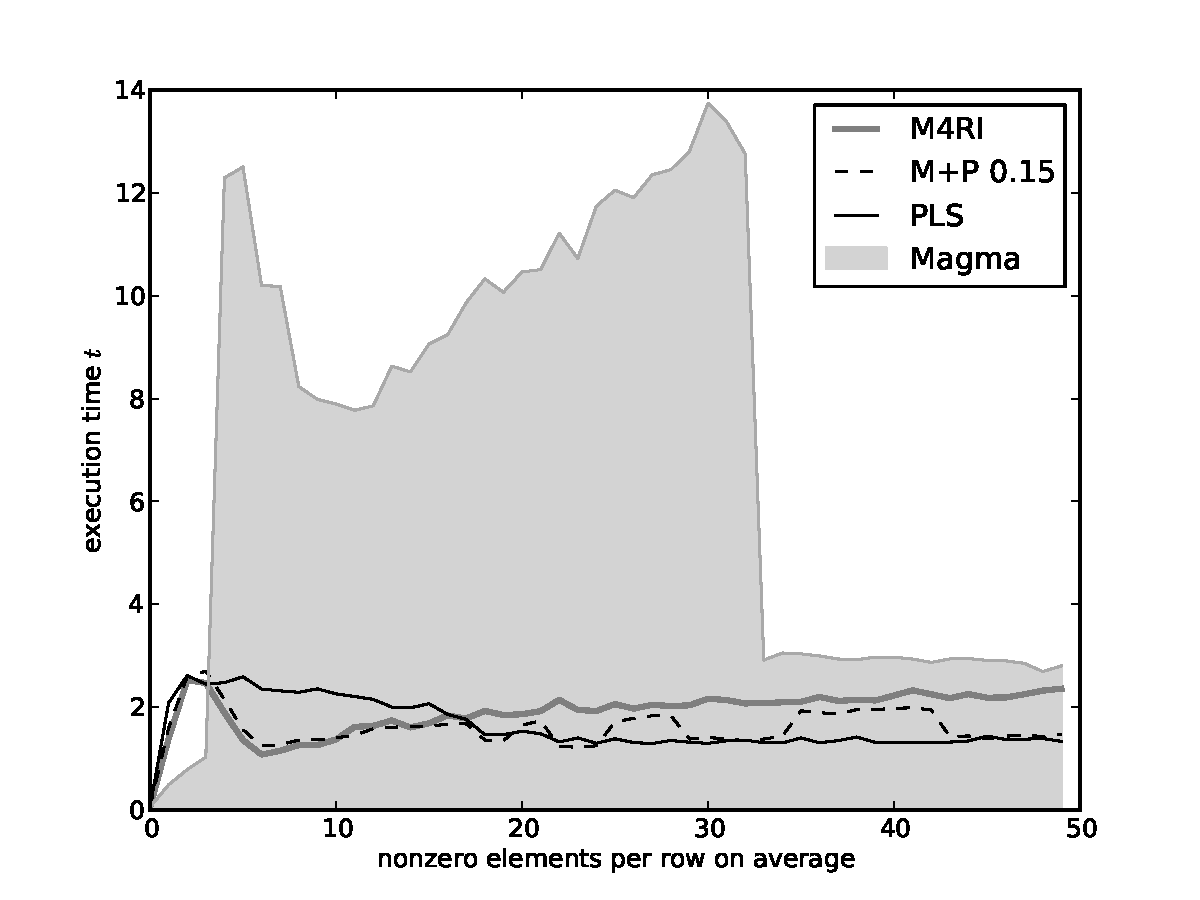
\includegraphics[width=0.9\textwidth]{./pluq-m4ri-magma-10000-prai243-20100409.pdf}
 \caption{Sensitivity to density for $n=10^4$ on 2.6Ghz \Opteron}
 \label{fig:sparse-m4ri}
\end{figure}

\section{Results}
\label{sec:pluq-results}
In Table~\ref{tab:pluq-random} we give average running time over ten trials for computing reduced row echelon forms of dense random $n \times n$ matrices over \GFZ. We compare the asymptotically fast implementation due to Allan Steel in \Magma, the cubic Gaussian elimination implemented by Victor Shoup in NTL, and both our implementations. Both the implementation in \Magma and our PLS decomposition reduce matrix decomposition to matrix multiplication. A discussion and comparison of matrix multiplication in the M4RI library and in \Magma can be found in Chapter~\ref{chapter:matmul}. In Table~\ref{tab:pluq-random} the column `PLS' denotes the complete running time for first computing the PLS decomposition and the computation of the reduced row echelon form from PLS. 

\begin{table}
\begin{footnotesize}
\begin{center}
\begin{tabular}{|c|r|r|r|r||r|r|r|r|}
\hline
 & \multicolumn{4}{|c||}{64-bit Linux, 2.6Ghz \Opteron} & 
\multicolumn{4}{|c|}{64-bit Linux, 2.33Ghz \Xeon (E5345)}\\
\hline
$n$             &  {\Magma} &   {NTL} &   {M4RI} &    {PLS}& {\Magma} &   {NTL} &   {M4RI} &    {PLS}\\
             & {2.15-10} &   5.4.2 & 20090105 & 20100324& {2.16-7} &   5.4.2 & 20100324 & 20100324\\
\hline
$10,000$ &   3.351s &   18.45s &   2.430s &   1.452s&   2.660s &  12.05s &   1.360s &   0.864s\\
$16,384$ &  11.289s &   72.89s &  10.822s &   6.920s&   8.617s &  54.79s &   5.734s &   3.388s\\
$20,000$ &  16.734s &  130.46s &  19.978s &  10.809s&  12.527s & 100.01s &  10.610s &   5.661s\\
$32,000$ &  57.567s &  479.07s &  83.575s &  49.487s&  41.770s & 382.52s &  43.042s &  20.967s\\
$64,000$ & 373.906s & 2747.41s & 537.900s & 273.120s& 250.193s &      -- & 382.263s & 151.314s\\

\hline
\end{tabular}
\caption{RREF for random matrices}
\label{tab:pluq-random}
\end{center}
\end{footnotesize}
\end{table}

In Table~\ref{tab:pluq-practice} we give running times for matrices as they appear when solving non-linear systems of equations. The matrices HFE 25, 30 and 35 were contributed by Michael Brickenstein and appear during a Gröbner basis computation of HFE systems using \PolyBoRi. The Matrix MXL was contributed by Wael Said and appears during an execution of the MXL2 algorithm \cite{mxl2} for a random quadratic system of equations. We consider these matrices within the scope of this work since during matrix elimination the density quickly increases and because the input matrices are already dense enough to expect one non-zero element per 128-bit wide SSE2 XOR on average. The columns `M+P $0.xx$' denote the hybrid algorithms which start with M4RI and switch over to PLS based echelon form computation once the density of the remaining part of the matrix reaches 15\% or 20\% respectively.
We note that the relative performance of the M4RI and the PLS algorithm for these instances depends on particular machine configuration. To demonstrate this we give a set of timings for the Intel \Xeon X7460 machine \texttt{sage.math} in Table~\ref{tab:pluq-practice}. Here, PLS is always faster than M4RI, while on a \Xeon E5345 M4RI wins for all HFE examples. We note that \Magma is not available on the machine \texttt{sage.math}\footnote{Purchased under National Science Foundation Grant No. DMS-0821725.}.
The HFE examples show that the observed performance regression for sparse matrices does have an impact in practice and that the hybrid approach does look promising for these instances.

\begin{table}
\begin{footnotesize}
\begin{center}
\begin{tabular}{|c|c|r|r|r|r|r|r|}
\hline
& & & \multicolumn{5}{|c|}{64-bit Fedora Linux, 2.33Ghz \Xeon (E5345)}\\
\hline
Problem & Matrix                 & Density &  Magma   &     M4RI &       PLS &  M+P 0.15 &  M+P 0.20\\
        & Dimension              &         &  2.16-7 &  20100324 &  20100324 &  20100429 &  20100429\\
\hline        
 HFE 25 & $12,307 \times 13,508$ &   0.076 &    3.68s &    1.94s &     2.09s &    2.33s &   2.24s\\
 HFE 30 & $19,907 \times 29,323$ &   0.067 &   23.39s &   11.46s &    13.34s &   12.60s &  13.00s\\
 HFE 35 & $29,969 \times 55,800$ &   0.059 &      --  &   49.19s &    68.85s &   66.66s &  54.42s\\
 MXL    & $26,075 \times 26,407$ &   0.185 &    55.15 &   12.25s &     9.22s &    9.22s &  10.22s\\
\hline
\hline
& & & \multicolumn{5}{|c|}{64-bit Ubuntu Linux, 2.66Ghz \Xeon (\texttt{sage.math})}\\
\hline
Problem & Matrix                 & Density & &      M4RI &       PLS &   M+P 0.15 & M+P 0.20\\
        & Dimension              &         & &  20100324 &  20100324 &   20100429 & 20100429\\
\hline        
 HFE 25 & $12,307 \times 13,508$ &   0.076 & &  2.24s &        2.00s &      2.39s &    2.35s\\
 HFE 30 & $19,907 \times 29,323$ &   0.067 & & 27.52s &       13.29s &     13.78s &    22.9s\\
 HFE 35 & $29,969 \times 55,800$ &   0.059 & &115.35s &       72.70s &     84.04s &  122.65s\\
 MXL    & $26,075 \times 26,407$ &   0.185 & & 26.61s &        8.73s &      8.75s &   13.23s\\
\hline
\hline
& & & \multicolumn{5}{|c|}{64-bit Debian/GNU Linux, 2.6Ghz \Opteron)}\\
\hline
Problem & Matrix                 & Density &  Magma   &     M4RI &        PLS &  M+P 0.15 &  M+P 0.20\\
        & Dimension              &         &  2.15-10 &  20100324 &  20100324 &  20100429 &  20100429\\
\hline        
 HFE 25 & $12,307 \times 13,508$ &   0.076 &   4.57s &    3.28s &       3.45s &   3.03s &   3.21s\\
 HFE 30 & $19,907 \times 29,323$ &   0.067 &  33.21s &   23.72s &      25.42s &  23.84s &  25.09s\\
 HFE 35 & $29,969 \times 55,800$ &   0.059 & 278.58s &  126.08s &     159.72s & 154.62s & 119.44s\\
 MXL    & $26,075 \times 26,407$ &   0.185 &  76.81s &   23.03s &      19.04s &  17.91s &  18.00s\\
\hline
\end{tabular}
\caption{RREF for matrices from practice.}
\label{tab:pluq-practice}
\end{center}
\end{footnotesize}
\end{table}


\part{\texorpdfstring{Gröbner}{Groebner} Basis Algorithms}
\label{part:gb}

\chapter{\texorpdfstring{Gröbner}{Groebner} Bases}
\label{chapter:groebner}
In this chapter the basic concepts of ideals in commutative multivariate polynomial rings and their Gröbner bases are discussed. The main purpose of this chapter is to motivate and present Buchberger's original algorithm for computing Gröbner bases.

The end of this chapter is a brief discussion how Gröbner bases are useful for solving systems of polynomial equations because it is the main application in this work.

This chapter is an extended and revised version of a chapter in the author's Diplomarbeit~\cite{Albrecht2007} later published as \cite{albrecht:cryptologia08}. 

For a more thorough introduction to the matters discussed in this chapter we point the reader to
\begin{itemize}
\item ``Ideals, Varieties, and Algorithms'' by Cox, Little, and O'Shea~\cite{Cox2005},
\item ``Gröbner Bases -- A Computational Approach to Commutative Algebra'' by Becker and Weispfenning~\cite{Becker1991} and 
\item ``Computational Commutative Algebra`` by Kreuzer and Robbiano~\cite{Kreuzer2000}.
\end{itemize}


\section{Notation}
The following notation and conventions are used throughout this text:
\begin{itemize}
\item We start counting at zero by default.
\item $\F$ is a field, not necessarily algebraically closed. $\overline{\F}$ represents the algebraic closure of $\F$. In source code listings we usually use {\tt K} to denote the field to avoid confusion with $F$ defined below.
\item $\F_{p}$ is the finite field of order $p$ with $p$ prime; $\F_{p^n}$ the finite extension field of degree $n$ over $\F_{p}$.
\item $\Z$ is the ring of integers; $\Z_{\geq 0}$ are the integers $\geq 0$.
\item $P$ is a polynomial ring $\F[x_0,\ \dots\ ,x_{n-1}]$ in the variables $x_0,\dots,x_{n-1}$.
\item $F = (f_0, \dots, f_{m-1})$ is an ordered list of polynomials in $P$; we denote by $\{f_0,\dots,f_{m-1}\}$ a set of unordered polynomials $f_0,\dots,f_{m-1}$.
 \item We call $m= x_0^{\alpha_0} x_1^{\alpha_1} \dots x_{n-1}^{\alpha_{n-1}}$ with $\alpha_i \in \Z_{\geq 0}$ a monomial and $t = c \cdot m$ with $c
\in \F$ a term. Note that some authors such as \cite{Becker1991} switch the definition of terms and monomials used here.

\item If $m = x_0^{\alpha_0} x_1^{\alpha_1} \dots x_{n-1}^{\alpha_{n-1}}$ is a monomial, we call $\alpha_0, \alpha_1, \dots \alpha_{n-1}$ its \emph{exponent vector}: $$\expvec(m) = \alpha_0, \alpha_1, \dots \alpha_{n-1}.$$

\item $M(f)$ is the set of monomials that appear in the polynomial $f$ and $T(f)$ the set of terms that appear in the same polynomial $f$. We extend this
definition to sets of polynomials $F = f_0, \dots, f_{m-1}$: $M(F) = \bigcup_{i=0}^{m-1} M(f_i)$ and $T(F) = \bigcup_{i=0}^{m-1} T(f_i)$

\item $\deg(m)$ is the degree of the monomial $m = x_0^{\alpha_0} x_1^{\alpha_1} \dots x_{n-1}^{\alpha_{n-1}}$ defined as $\sum_{i=0}^{n-1} \alpha_i$. We extend this definition to polynomials such that $\deg(f)$ for $f = \sum c_i m_i$ is defined as $\max\{\deg(m_i)\}$. We define $\deg(\alpha)$ as $\deg(m)$ for $\alpha = \expvec(m)$.
\item $A[i,j]$ represents the element in row $i$ and column $j$ in the matrix
$A$.
\item $f \mod g$ denotes the result of the modulo operation $f$ modulo $g$.
\end{itemize}

Whenever suitable, examples are provided to illustrate theorems, algorithms and propositions. Also, if possible, source code snippets are provided to reproduce examples in the mathematical software \Sage~\cite{sage}. \Sage is an open-source mathematics software that aims to provide a ``viable alternative to Magma, Maple, Mathematica and Matlab.''

For example, consider the following set of polynomials in $\F_{127}[x,y,z]$.
\begin{align*}
f_0 &= 81 z^{2} + 51 x + 125 z + 38\\
f_1 &= 76 x y + 80 y^{2} + 49 x z + 62 y z + 45 z^{2}\\
f_2 &= 122 x^{2} + 106 y z + 78 z^{2} + 48 x + 112 y
\end{align*}
This example can be constructed in \Sage as follows:
\begin{lstlisting}
sage: K = GF(127)
sage: P.<x,y,z> = PolynomialRing(K)
sage: f0 = -46*z^2 + 51*x - 2*z + 38
sage: f1 = -51*x*y - 47*y^2 + 49*x*z + 62*y*z + 45*z^2
sage: f2 = -5*x^2 - 21*y*z - 49*z^2 + 48*x - 15*y
\end{lstlisting}

\section{Monomial Orderings}
When we consider univariate polynomials it is straight-forward to determine which monomial is the largest and which is the smallest. Once we consider multivariate polynomials, things are not as straight-forward anymore. Thus, we attach a monomial ordering or term ordering to a ring which encodes how we compare monomials.

\begin{definition}[Monomial Ordering \cite{Cox2005}]
A monomial ordering on $\F[x_0,\dots,x_{n-1}]$ is any relation $>$ on $\Z_{\geq 0}^n$, or equivalently, any relation on the set of monomials $x^\alpha$,$\alpha \in \Z_{\geq 0}^n$, satisfying:
\begin{enumerate}
 \item $>$ is a total (or linear) ordering on $\Z_{\geq 0}^n$.
 \item If $\alpha > \beta$ and $\gamma$ $\in \Z_{\geq 0}^n$ then $\alpha + \gamma > \beta + \gamma$.
 \item $>$ is a well-ordering on $\Z_{\geq 0}^n$. This means that every non-empty subset of $\Z_{\geq 0}^n$ has a smallest element under $>$.
\end{enumerate}

\end{definition}

Two of the most used monomial orderings are the ``lexicographical'' and the ``degree reverse lexicographical'' ordering.

\begin{definition}[Lexicographic ordering \emph{lex}]
\label{def:lex}
Let the exponent vector $\alpha = (\alpha_0, \dots, \alpha_{n-1})$ and $\beta = (\beta_0, \dots, \beta_{n-1})$ $\in \field{Z}_{\geq 0}^n$. We say
$\alpha \underset{lex}{>} \beta$ if, in the vector difference $\alpha - \beta \in \field{Z}^n$, the left-most non-zero entry is positive.
We will write $x^\alpha \underset{lex}{>} x^\beta$ if $\alpha \underset{lex}{>} \beta$. 
\end{definition}

We will show later in this chapter that \emph{lex} is an order which allows to ``read'' the solution to a multivariate polynomial equation system from the Gröbner basis. This is, because \emph{lex} is an \emph{elimination ordering}. But in practice computing a lexicographical Gröbner basis is usually less efficient than computing a \emph{degree reverse lexicographic} Gröbner basis:

\begin{definition}[Degree reverse lexicographic ordering \emph{degrevlex}] 
\label{def:degrevlex}
Let the exponent vector $\alpha = (\alpha_0, \dots, \alpha_{n-1})$ and $\beta = (\beta_0, \dots, \beta_{n-1})$ $\in \field{Z}_{\geq 0}^n$.
We say $\alpha \underset{degrevlex}{>} \beta$ if either
\begin{itemize}
 \item $\deg( \alpha ) > \deg(\beta )$  or
 \item $\deg(\alpha) = \deg(\beta)$ and the rightmost non-zero entry in the vector difference $\alpha - \beta \in \Z^n$ is negative.
\end{itemize}
We will write $x^\alpha \underset{degrevlex}{>} x^\beta$ if $\alpha \underset{degrevlex}{>} \beta$.
\end{definition}

We will also need block orderings later in this work which are elimination orderings potentially ``mixed'' with other monomial orderings.

\begin{definition}[Block or product ordering] 
\label{def:blockorder}
Let $x = (x_0, \ldots, x_{n-1})$ and  $y = (y_0, \ldots, y_{m-1})$ be two ordered sets of variables, $<_1$ a monomial ordering on $\F[x_0,\dots,x_{n-1}]$ and $<_2$ a monomial ordering on $\F[y_0,\dots,y_{m-1}]$. We say that $x^a y^b < x^A y^B$ with respect to the the block ordering (or product ordering) $(<_1,<_2)$ on $\F[x_0,\dots,x_{n-1},y_0,\dots,y_{m-1}]$ if either

\begin{itemize}
 \item $x^a <_1 x^A$  or 
 \item $x^a = x^A$ and $y^b <_2 y^B$.
\end{itemize}

Inductively one defines the product ordering of more than two monomial orderings.
\end{definition}

We will simply write $x > y$ if it is clear from the context which ordering we are referring to. We can extend monomial orderings to polynomials by comparing the largest monomials first and compare smaller monomials only if these are equal.

For example consider the polynomial 
\[f = 1 + y_{0} + x_{2} + x_{1} + x_{0} + x_{0}x_{1} \in \F[y_0,x_0,x_1,x_2].\]
With respect to the lexicographical monomial ordering and $y_{i} > x_{i}$ we have that the leading monomial of $f$ is $y_{0}$ but with respect to the degree reverse lexicographical ordering the leading monomial is $x_{0}x_{1}$ because it has degree two. If we consider the block ordering with the two blocks $y_0$ and $x_0,x_1,x_2$ and choose \emph{degrevlex} in both blocks we have that $y_0$ is the leading monomial.

Monomial orderings are assigned to multivariate polynomial rings in \Sage by using the \verb|order| keyword:

\begin{lstlisting}
sage: P.<y0,x0,x1,x2> = PolynomialRing(QQ, order='lex')
sage: f =  1 + y0 + x2 + x1 + x0 + x0*x1
sage: f.lm()
y0

sage: P.<y0,x0,x1,x2> = PolynomialRing(QQ, order='degrevlex')
sage: f =  1 + y0 + x2 + x1 + x0 + x0*x1
sage: f.lm()
x0*x1

sage: T = TermOrder('degrevlex',1) + TermOrder('degrevlex',3)
sage: P.<y0,x0,x1,x2> = PolynomialRing(QQ, order=T)
sage: f =  1 + y0 + x2 + x1 + x0 + x0*x1
sage: f.lm()
y0
\end{lstlisting}

We denote the largest monomial in a polynomial $f$ as the leading monomial $\LM(f)$, its coefficient as the leading coefficient $\LC(f)$ and their product as the leading term $\LT(f) = \LC(f)\cdot \LM(f)$.

\section{\texorpdfstring{Gröbner}{Groeber} Bases}

We are interested in ideals of multivariate polynomial rings and their bases.

\begin{definition}[Ideal]
\label{def:ideal}
A subset $I \subset P$ is an ideal if it satisfies:
\begin{enumerate}
\item $0 \in I$;
\item If $f$, $g \in I$, then $f + g \in I$;
\item If $f \in I$ and $h \in P$, then $h \cdot f \in I$.
\end{enumerate}
\end{definition}



\begin{definition}
Let $f_0 ,\dots , f_{m-1}$ be polynomials in $P$ . Define the set
\[
\langle f_0 , \dots , f_{m-1}\rangle = \left\{ \sum_{i=0}^{m-1} h_i f_i : h_0 ,\dots , h_{m-1} \in P \right\}.
\]
This set $I$ is an ideal called the ideal generated by $f_0, \dots, f_{m-1}$.
\end{definition}

\begin{definition}[Leading Monomial Ideal]
Let $I$ be an ideal $\subset P$ and define the set
\[
 \left\{ \LM(f_i) \mid f_i \in I\right\}.
\]
We call the ideal spanned by this set the leading monomial ideal of $I$ and denote it as $\langle \LM(I) \rangle \subset P$.
\end{definition}

If there exists a finite set of polynomials in $P$ that generates a given ideal, this set is called a basis. The Hilbert basis theorem states that every ideal in $P$ is finitely generated:

\begin{theorem}[Hilbert's Basis Theorem]
\label{theorem:hilbbase}
Every ideal $I \subset P$ has a finite generating set. That is, $I = \langle
f_0, \dots, f_{m-1} \rangle$ for some $f_0,
\dots, f_{m-1} \in I$.
\end{theorem}

\begin{citeproof} 
See \cite[p. 74]{Cox2005}.
\end{citeproof}

Note that most ideals have many different bases.

Hilbert's Basis Theorem has important consequences for Gröbner basis calculations. One is that a nested
increasing sequence of ideals $I_0 \subset I_1 \subset \dots$ in $P$ stabilizes at a certain point in time. Explicitly:

\begin{theorem}[Ascending Chain Condition] 
\label{theorem:acc}
Let 
\[
I_0 \subset I_1 \subset I_2 \subset \dots
\]
be an ascending chain of ideals in $P$. Then there exists an $N \geq 1$ such that 
\[
I_{N} = I_{N+1} = I_{N+2} = \dots\ .
\]
\end{theorem}

\begin{citeproof}
See \cite[p.76]{Cox2005}.
\end{citeproof}

\begin{definition}[Noetherian Ring]
A ring for which the Ascending Chain Condition for ideals holds is called a \emph{noetherian} ring.
\end{definition}


Gröbner bases are defined as:
\begin{definition}[Gröbner Basis]
Let $I$ be an ideal of $\F[x_0,\dots,x_{n-1}]$ and fix a monomial ordering. A finite subset $$G = \{g_0 ,\dots , g_{m-1} \} \subset I$$  is said to be a \emph{Gröbner basis} or standard basis of $I$ if
\[
\langle \LM(g_0 ), \dots , \LM(g_{m-1})\rangle = \langle \LM(I) \rangle.
\]
\end{definition}

Thus for every $f_i \in I$ we have that $\LM(f_i)$ is divisible by some $\LM(g_i) \in G$.

\begin{example}
For instance a Gröbner basis with respect to the \emph{degrevlex} monomial ordering and $x > y > z$ for the example presented earlier
\begin{align*}
f_0 &= 81 z^{2} + 51 x + 125 z + 38\\
f_1 &= 76 x y + 80 y^{2} + 49 x z + 62 y z + 45 z^{2}\\
f_2 &= 122 x^{2} + 106 y z + 78 z^{2} + 48 x + 112 y
\end{align*}
is:
\begin{align*}
g_0 &= y^{3} + 66 y^{2} z + 72 y^{2} + 98 x z + 64 y z + 56 x + 16 y + 38 z + 53,\\
g_1 &= x^{2} + 55 y z + 99 x + 3 y + 57 z + 60,\\
g_2 &=x y + 108 y^{2} + 9 x z + 71 y z + 57 x + 65 z + 35,\\
g_3 &=z^{2} + 90 x + 116 z + 82.
\end{align*}
\end{example}

This Gröbner basis was obtained by the following sequence of commands in \Sage:

\begin{lstlisting}
sage: P.<x,y,z> = PolynomialRing(GF(127),order='degrevlex')
sage: f = -46*z^2 + 51*x - 2*z + 38
sage: g = -51*x*y - 47*y^2 + 49*x*z + 62*y*z + 45*z^2
sage: h= -5*x^2 - 21*y*z - 49*z^2 + 48*x - 15*y
sage: I = Ideal(f,g,h)
sage: I.groebner_basis()
[y^3 - 61*y^2*z - 55*y^2 - 29*x*z - 63*y*z + 56*x + 16*y + ..., 
 x^2 + 55*y*z - 28*x + 3*y + 57*z + 60, 
 x*y - 19*y^2 + 9*x*z - 56*y*z + 57*x - 62*z + 35, 
 z^2 - 37*x - 11*z - 45]
\end{lstlisting}

\begin{definition}[\cite{Cox2005}]
Fix a monomial order $>$ on $\Z_{\geq 0}^n$ and let $F = (f_0, \dots,f_{s-1})$ be an ordered $s$-tuple of polynomials in $\F[x_0,\dots,x_{n-1}]$. Then every $f \in \F[x_0,\dots,x_{n-1}]$ can be written as \[ f = a_0f_0 + \cdots + a_{s-1}f_{s-1} + r,\] where $a_i,r \in \F[x_0,\dots,x_{n-1}]$ and either $r=0$ or $r$ is a linear combination, with coefficients in $\F$, of monomials, none of which is divisible by any of $\LM(f_0),\dots,\LM(f_{s-1})$. We call $r$ a \emph{remainder} of $f$ on division by $F$. Furthermore, if $a_if_i \neq 0$, then we have \[\expvec(\LM(f)) \geq \expvec(\LM(a_if_i)).\] We write
\[\overline{f}^F = r.\]
\end{definition}

\begin{citeproof}
See \cite[p.62ff]{Cox2005}. 
\end{citeproof}

An algorithm to compute $a_0,\dots,a_{s-1}$ is given in Algorithm~\ref{alg:long_division}.

\begin{algorithm}[ht]
\KwIn{$(f_0,\dots,f_{s-1},f)$ -- a $s+1$-tuple of polynomials $\in P$.}
\KwResult{$a_0,\dots,a_{s-1},r$ -- a $s+1$-tuple of polynomial $\in P$.}
\SetKw{KwAnd}{and}

\Begin{
$a_i \longleftarrow 0$; $r \longleftarrow 0$; $p \longleftarrow f$\;
\While{$p = 0$}{
  $i \longleftarrow 0$\;
  $divisionoccured \longleftarrow False$\;
  \While{$i < s$ \KwAnd $divisionoccured = False$}{
    \If{$\LT(f_i) \mid \LT(p)$}{
       $a_i \longleftarrow a_i + \LT(p)/\LT(f_i)$\;
       $p \longleftarrow p - \LT(p)/\LT(f_i)f_i$\;
    }
    \Else{
       $i \longleftarrow i + 1$\;
    }
  }
  \If{$divisionoccured = False$}{
      $r \longleftarrow r + \LT(p)$\;
      $p \longleftarrow p - \LT(p)$\;
  }
}
\Return{$a_0,\dots,a_{s-1},r$}\;
}
\caption{\textsc{Long Division}} 
\label{alg:long_division}
\end{algorithm} 




Gröbner bases have several interesting properties: the remainder $r$ of the division of any $f \in P$ by $G$ is
unique and \emph{reduced} Gröbner bases are a unique representation of an ideal with respect to a monomial ordering.

\begin{definition}[Reduced Gröbner Basis]
A \emph{reduced Gröbner basis} for a polynomial ideal $I$ is a
Gröbner basis $G$ such that:
\begin{enumerate}
\item $\LC(f) = 1$ for all $f \in G$;
\item $\forall f \in G, \not\exists\ m \in M(f)$\ such that $m \in \langle \LM(G
\setminus \{f\})\rangle$ .
\end{enumerate}
\end{definition}

By default, \Sage will always computes the reduced Gröbner basis when computing a Gröbner basis. If a Gröbner basis was obtained by other means, the function 
\begin{lstlisting}
MPolynomialIdeal.interreduced_basis()
\end{lstlisting}
can be used to compute the reduced Gröbner basis.
\begin{lstlisting}
sage: rgb = Ideal(gb).interreduced_basis()
\end{lstlisting}

Note that \Sage\ -- unlike other systems like \Singular~\cite{singular} -- does differentiate between tuples of polynomials and ideals. Ideals are first order objects in \Sage.

\section{Buchberger's Algorithm}
In 1965 Bruno Buchberger introduced the notion of a Gröbner basis and also a criterion to test whether a set of polynomials is a Gröbner basis. This criterion naturally leads to Buchberger's algorithm for computing a Gröbner basis from a given ideal basis. The main concepts of his criterion are
presented below.

Consider a set of polynomials $G = \{f_0,\dots,f_{m-1}\} \subset \F[x_0,\dots,x_{n-1}]$. If there exists any $m \in \langle \LM(I) \rangle$ with $$m \not\in \langle \LM(f_0),\ \dots\ ,\LM(f_{m-1})\rangle,$$ then $G$ is not a Gröbner basis for $\ideal{G}$; this follows from the definition of Gröbner bases. 

In order obtain a candidate for such $m$, we may choose two elements $f_i$ and $f_j$ of $G$ and compute \[s = ax^\alpha f_i - bx^\beta f_j.\]
We know that $\LM(ax^\alpha f_i\ -\ bx^\beta f_j) \in \langle\LM(I)\rangle$ because $ax^\alpha f_i\ -\ bx^\beta f_j\ \in\ I$. Now assume that in $s$ the terms $ax^\alpha\LT(f_i)$ and $bx^\beta\LT(f_j)$ ($a,b \in \F$) cancel each other out. If as a result $\LM(ax^\alpha f_i\ -\ bx^\beta f_j)$ is not in the ideal $\langle\LM(f_0), \dots ,\LM(f_{t-1})\rangle$ we know that $G$ cannot be a Gröbner basis. 


S-polynomials are a (in fact: \emph{the}) way to construct the required cancellations of leading terms:

\begin{definition}[S-Polynomial]
\hfill\par
\label{def:spolynomials}
Let $f,g\ \in\ \F[x_0,\dots,x_{n-1}]$ be non-zero polynomials.
\begin{enumerate}
\item If $\alpha =\expvec(\LM(f))$ and $\beta = \expvec(\LM(g))$ then let $\gamma\ =\ (\gamma_0,\ \dots\ ,\gamma_{n-1})$ where 
$\gamma_i = \max(\alpha_i,\beta_i) \textnormal{ for every } i\ < n.$ We then have that $x^\gamma$ is the least common multiple of
$\LM(f)$ and $\LM(g)$, written as $$x^\gamma\ =\ \LCM(\LM(f),\LM(g)).$$  
\item The S-polynomial of $f$ and $g$ is defined as
\begin{align*}
S(f,g)\ =\ \frac{x^\gamma}{\textsc{LT}(f)}\cdot f\ -\
\frac{x^\gamma}{\textsc{LT}(g)}\cdot g.
\end{align*}
\end{enumerate}
We call $f$ and $g$ the \emph{generators} of $S(f,g)$ and $\frac{x^\gamma}{\textsc{LT}(f)}\cdot f$  and $\frac{x^\gamma}{\textsc{LT}(g)}\cdot g$ the \emph{components} of $S(f,g)$. Sometimes, it is beneficial to consider the products in the components unevaluated, namely as the tuples
$(\frac{x^\gamma}{\textsc{LT}(f)}, f)$ and $(\frac{x^\gamma}{\textsc{LT}(g)}, g)$. We call the tuple $(f,g)$ a \emph{critical pair}.
\end{definition}

The following example illustrates that $S(f_i,f_j)$ is constructed in a way to allow cancellation of leading terms.

\begin{example}
Let $f_0\ =\ x^3\ -\ 2xy$ and $f_1\ =\ x^2y\ -\ 2y^2\ +\ x$. The leading monomials with respect to \emph{degrevlex} and $x > y$ are
$\LM(f_0)\ =\ x^3$ and $\LM(f_1)\ =\ x^2y$ and thus $x^\gamma\ =\ x^3y$. The S-polynomial is:
\begin{eqnarray*}
S(f_0,f_1)\ &=&\ \dfrac{x^\gamma}{\LT(f_1)}\ \cdot\ f_1\ -\
\dfrac{x^\gamma}{\LT(f_2)}\ \cdot\ f_2\\
S(f_0,f_1)\ &=&\ \dfrac{x^3y}{x^3}\ \cdot\ (x^3\ -\ 2xy)\ -\
\dfrac{x^3y}{x^2y}\ \cdot\ (x^2y\ -\ 2y^2\ +\ x)\\
S(f_0,f_1)\ &=&\ y\ \cdot (x^3\ -\ 2xy)\ -\ \ x\ \cdot (x^2y\ -\ 2y^2\ +\ x)\\
S(f_0,f_1)\ &=&\ x^3y\ -\ 2xy^2\ -\ \ x^3y\ +\ 2xy^2\ -\ x^2\\
S(f_0,f_1)\ &=&\ -x^2
\end{eqnarray*}
\end{example}

The same example in Sage:

\begin{lstlisting}
sage: P.<x,y> = PolynomialRing(QQ,order='degrevlex')
sage: f0 = x^3 - 2*x*y
sage: f1 = x^2*y -2*y^2 + x
sage: (x^3*y)//x^3 * f0 - (x^3*y)//(x^2*y) * f1
-x^2
\end{lstlisting}

The educational \verb|sage.rings.polynomial.toy_buchberger| module also offers a function \verb|spol|:

\begin{lstlisting}
sage: from sage.rings.polynomial.toy_buchberger import spol
sage: spol(f0,f1)
-x^2
\end{lstlisting}


The following lemma states that whenever combinations of terms cancel each other out in a polynomial this cancellation may be accounted to S-polynomials.

\begin{lemma}
\label{lemma:cancel}
Let the leading term of every summand of \[s = \sum^{t-1}_{i=0} c_ix^{\alpha_i}g_i \in \F[x_0,\dots,x_{n-1}]\] with $c_i \in \F$, have the exponent vector 
\[\delta = \alpha_i\ +\ \expvec(\LM(g_i)) \in \mathbb{Z}^n_{\geq 0} \textnormal{ if } c_i\ \neq\ 0.\] If $\expvec(\LM(s))$ is smaller than $\delta$, then $s$ is a linear combination  of the S-polynomials $S(f_j,f_k)$ for $0 \leq j,k < t$ with coefficients $c_i$ in $\F$. Furthermore, each leading monomial of $S(f_j,f_k)$ has exponent vector $< \delta.$
\end{lemma}

\begin{citeproof}
See \cite[p.81ff]{Cox2005}.
\end{citeproof}

The key idea of Buchberger's constructive criterion for Gröbner bases is to use these S-polynom\-ials to construct new elements $S(f,g)$ in the ideal with smaller leading term than those of the components of $S(f,g)$. If such elements  can be found whose leading terms are not multiples of leading terms of
other elements already in the basis then the basis is not a Gröbner basis.

\begin{theorem}[Buchberger's Criterion]
\label{theorem:buchberger}
Let $I$ be an ideal. $G\ =\ \left\lbrace g_0,\ \dots\ ,g_{s-1}\right\rbrace$ is
a Gröbner basis for $I$, if and only if for all pairs $i \neq j$, the remainder $r$ of the division of $S(g_i,g_j)$
by $G$ (listed in some order) is zero, that is we have that $\overline{f}^{G} = 0$.
\end{theorem}

\begin{citeproof}
See \cite[p.82ff]{Cox2005}
\end{citeproof}

\begin{example}
Let $f_0\ =\ x^3\ -\ 2xy$ and $f_1\ =\ x^2y\ -\ 2y^2\ +\ x$. The S-polynomial is $-x^2$ which is not reducible by either
$LM(f_0) = x^3$ or $LM(f_1) = x^2y$. Thus, $(f_0,f_1)$ is not a Gröbner basis.
\end{example}

There is another -- related -- criterion which can be checked to verify if a given set of polynomials forms a Gröbner
basis or not. For that criterion the expression $f$ \emph{reduces to zero modulo} $G$ is needed.

\begin{definition}
\cite[p.100]{Cox2005} Fix a monomial order and let $G = \{g_0 ,\dots , g_{s-1} \} \subset P$ be an \emph{unordered} set of polynomials. Given a polynomial $f \in P$, we say that $f$ reduces to zero modulo G, written \[f  \underset{G}{\longrightarrow} 0,\] if $f$ can be written in the form \[f = a_0 g_0 + \dots + a_{s-1} g_{s-1} ,\] with $a_i \in P$ such that whenever $a_i g_i \not= 0$, we have \[\LM(f) \geq \LM(a_i g_i).\]
\end{definition}

Alternatively, we may express this concept using the notion of $t$-representations:

\begin{definition}[$t$-Representation]
Fix a monomial order and let $G = \{g_0 ,\dots , g_{s-1} \} \subset P$ be an \emph{unordered} set of polynomials and let $t$ be a monomial. Given a polynomial $f \in P$, we say that $f$ has a \emph{$t$-representation}  if $f$ can be written in the form \[f = a_0 g_0 + \dots + a_{s-1} g_{s-1} ,\] such that whenever $a_i g_i \not= 0$, we have  $a_i g_i \leq t.$ Furthermore, we have that $f  \underset{G}{\longrightarrow} 0$ if and only if $f$ has an $\LM(f)$-representation with respect to $G$.
\end{definition}

Please note, that $\overline{f}^G = 0$ implies $f \underset{G}{\longrightarrow} 0$ but the converse does not hold in general \cite[100ff]{Cox2005}. 

\begin{example}
Consider some $\field{F}[x,y]$ with the \emph{degree reverse lexicographical} monomial ordering and $f = xy^2 - x$ and $G= (xy + 1, y^2 - 1)$. The division
algorithm (cf. Algorithm~\ref{alg:long_division}) gives $f = xy^2 - x = y \cdot (xy + 1) + 0 \cdot (y^2 -1) + (-x - y)$ which implies $\overline{f}^G \neq 0$. On the other hand we can write $f = xy^2 - x = 0 \cdot (xy + 1) + x \cdot (y^2 - 1)$ which implies $f\underset{G}{\longrightarrow}0$.
\end{example}

Using this definition Buchberger's Criterion may be reformulated as follows:

\begin{theorem}
\label{thm:groebnerreducestozero}
A basis $G = \{g_0 ,\dots , g_{s-1} \}$ for an ideal $I$ is a Gröbner basis if and only if \[S(g_i,g_j)
\underset{G}{\longrightarrow} 0\]
for all $i \not= j$.
\end{theorem}

The proof of this theorem follows directly from the proof of Buchberger's criterion in \cite{Cox2005}.

Buchberger's criterion (Theorem~\ref{theorem:buchberger}) and the Ascending Chain Condition (Theorem~\ref{theorem:acc}) lead to the following algorithm for
computing Gröbner basis:

\begin{algorithm}[ht]
\KwIn{$F$ -- a finite subset of $P$}
\KwResult{a Gröbner basis for the ideal spanned by $F$}

\Begin{
$G \longleftarrow F$\;
$G_2 \longleftarrow \varnothing$\;
\While{$G_2 \neq G$}{
  $G_2 \longleftarrow G$\;
  \For{$f,g \in G_2 \times G_2$}{
      \If{$\LM(f)<\LM(g)$}{
       $ \tilde{s} \longleftarrow \overline{S(f,g)}^G$\;
       \lIf{$\tilde{s}\neq 0$}{add $\tilde{s}$ to $G$\;}
      }
   }
 }
 \Return{G}\;
}
\caption{Buchberger's Algorithm}
\label{alg:buchberger}
\end{algorithm}


The correctness and termination of this algorithm may be derived from the
following three observations:
\begin{enumerate}
\item At every stage of the algorithm, $G \subset I$ and $\langle G \rangle = I$ hold.
\item If $G_2 = G$ then $S(f, g) \underset{G}{\longrightarrow} 0$ for all $f, g \in G$ and, by Buchberger's criterion, $G$ is a Gröbner basis.
\item The equality $G_2 = G$ occurs in finitely many steps since the ideals $\ideal{\LM(G)}$, from successive iterations of the loop, form an ascending chain. Due to the Ascending Chain Condition (Theorem~\ref{theorem:acc}) this chain of ideals stabilizes after a finite number of iterations and at that moment $\ideal{\LM(G)} = \ideal{\LM(G_2)}$ holds, which implies $G_2 = G$.
\end{enumerate}

A straight-forward implementation of Buchberger's algorithm in \Sage is given below:

\begin{lstlisting}
spol = lambda f,g: LCM(f.lm(),g.lm())//f.lt()*f - \
                   LCM(f.lm(),g.lm())//g.lt()*g
def buchberger(F):
  G = set(F)
  G2 = set()
  while G2!=G:
    G2 = copy(G)
    for f,g in cartesian_product_iterator([G2,G2]):
        if f<g:
          s = spol(f,g).reduce(G2)
          if s != 0:
            G.add(s)
  return G
\end{lstlisting}

It is implemented as \verb|buchberger| in \verb|sage.rings.polynomial.toy_buchberger| by the author:

\begin{lstlisting}
sage: P.<x,y> = PolynomialRing(QQ, order='degrevlex')
sage: f0 = x^3 - 2*x*y                                       
sage: f1 = x^2*y -2*y^2 + x  
sage: buchberger(Ideal(f0,f1))
[x^2*y - 2*y^2 + x, -2*x*y, -2*y^2 + x, x^2, x^3 - 2*x*y]
\end{lstlisting}

Even though this algorithm terminates eventually it is well known \cite[p.511ff]{Becker1991} that its runtime is not polynomial in the number of variables, as the intermediate bases $G_2$ grow exponentially during the calculations. In particular, we have the following theorem:

\begin{theorem}[\cite{faugere-ars-2004}]
Let $I$ be an ideal in $\F_q[x_0,\dots,x_{n-1}]$ generated by polynomials $f_0,\dots,f_{n-1}$ of degrees $d_0,\dots,d_{n-1}$ respectively. Assume the ideal $I$ is zero-dimensional (defined in Section~\ref{sec:solvingmq}).
\begin{itemize}
 \item A Gröbner basis computation for a \emph{lexicographical} monomial order reaches at most degree $D \leq \prod_{i=0}^{n-1} d_i$.
 \item A Gröbner basis computation for a \emph{degree reverse lexicographical} monomial order reaches at most degree $D \leq 1 - n + \sum_{i=0}^{n-1} d_i$.
\end{itemize}
\end{theorem}

Buchberger's algorithm leaves a lot of freedom when implemented. The runtime can be reduced by applying a variety of improvements:
\begin{itemize}
\item The order in which the critical pairs $f,g$  are selected influences running time.
\item One can use Buchberger's criteria to avoid useless reductions to zero.
\item Algorithms exist \cite{fglm,Collart1997} to convert a Gröbner basis (of a zero-dimensional ideal) in one monomial order to a Gröbner basis in another monomial order, thus we may compute with respect to the degree reverse lexicographical ordering first and then convert the result to the lexicographical ordering.
\end{itemize}

Buchberger himself gave two criteria to avoid useless reductions to zero.

\begin{definition}[Buchberger's First Criterion \cite{Becker1991}]
Let $f,g \in \F[x_0,\dots,x_{n-1}]$ with disjoint leading terms, i.e.\ $GCD(\LM(f),\LM(g)) = 1$. Then $S(f,g) \underset{\{f,g\}}{\longrightarrow} 0$.
\label{def:buchberger_first_criterion}
\end{definition}

\begin{citeproof}
See \cite[p.222]{Becker1991}. 
\end{citeproof}

\begin{definition}[Buchberger's Second Criterion \cite{Becker1991}]
Let $F$ be a finite subset of $\F[x_0,\dots,x_{n-1}]$ and $g_0, p, g_1 \in \F[x_0,\dots,x_{n-1}]$ such that the following hold:
\begin{enumerate}
 \item $\LM(p) \mid \LCM(\LM(g_0),\LM(g_1))$, and
 \item $S(g_i,p)$ has a $t_i$-representation w.r.t. $F$ with \[t_i < \LCM(\LM(g_i),\LM(p)) \textnormal{ for } i = 0,1.\]
\end{enumerate}
Then $S(g_0,g_1) \underset{F}{\longrightarrow} 0$.
\label{def:buchberger_second_criterion}
\end{definition}

\begin{citeproof}
See \cite[p.224ff]{Becker1991}. 
\end{citeproof}

The standard instantiation of those two criteria is the \emph{Gebauer-Möller installation} \cite{Gebauer1988} which is implemented in most computer algebra systems that implement Gröbner basis algorithms. Later in this text we will discuss other improved Gröbner basis algorithms such as $F_4$ (Chapter~\ref{chapter:f4}) and $F_5$ (Chapters~\ref{chapter:f5matrix} and \ref{chapter:f5}), both due to Jean-Charles Faugère.

We will also consider later the computation of Gröbner bases up to some degree $D$. That is, we run, for example, Buchberger's algorithm but discard any S-polynomials with a degree $> D$. If all input polynomials are homogeneous, Gröbner bases up to a degree $D$ are well-defined. However, in the affine case this is not true since the degree during a polynomial reduction may drop. Thus, the computation up to some degree $D$ in the affine case is little more than a random interruption of the Gröbner basis algorithm.

\section{Solving Polynomial Systems with Gröbner Bases}
\label{sec:solvingmq}

This section is concerned with explaining the relationship between solving systems of polynomial equations and Gröbner bases. First we need to formally define the
concept of a solution to a system of polynomials.

\begin{definition}
Given a field $\F$ and a positive integer $n$, we define the $n$-dimensional
\emph{affine space} over $\F$ to be the set
\[
\F^n = \{(a_0 , \dots , a_{n-1} ) : a_0 , \dots , a_{n-1} \in \F\} .
\]
\end{definition}
Evaluating a polynomial $f \in \F[x_0,\dots,x_{n-1}]$ at $(a_0 , \dots , a_{n-1} ) \in \field{K}^n$, where $\field{K}$ is some algebraic extension of $\F$, is a function
\[
f : \field{K}^n \longrightarrow \field{K},
\]
where every $x_i$ is replaced by $a_i \in \field{K}$ for $0 ≤ i < n$.

The set of all solutions in $\field{K}^n$ to a system of equations
\[
f_0(x_0 ,\dots , x_{n-1}) = 0, \dots, f_{m-1} (x_0 , \dots , x_{n-1} ) = 0
\]
is called an \emph{affine $\F$-variety}, formally defined as follows.
\begin{definition}
Let $\F$ be a field, $\field{K}$ some algebraic extension of $\F$ and $f_0 ,\dots , f_{m-1}$ be polynomials in $\F[x_0,\ \dots\ ,x_{n-1}]$, that is all coefficients are in $\F$. We define
\[
V(f_0 , \dots , f_{m-1}) = \{(a_0 ,\dots , a_{n-1} ) \in \field{K}^n : f_i(a_0 , \dots , a_{n-1} ) = 0\textnormal{ for all }0 \leq i < m\}.
\]
We call $V(f_0 ,\dots , f_{m-1})$ the affine $\F$-variety defined by $f_0 ,\dots , f_{m-1}$.
\end{definition}

Note that the $\F$ in ``affine $\F$-variety'' refers to the field of the coefficients not the solution.

\begin{definition}[PoSSo]
Given a finite set $F = \{f_0, \dots, f_{m-1}\} \subset \F[x_0,\dots,x_{n-1}]$ of multivariate polynomials in $P$ we call PoSSo the problem of finding
the affine variety of $F$.
\end{definition}

\begin{lemma}
If $f_0 ,\dots , f_{s-1}$ and $g_0 ,\dots , g_{t-1}$ are bases of the same ideal in $P$,
so that \[\langle f_0 ,\dots, f_{s-1}\rangle = \langle g_0 ,\dots , g_{t-1}\rangle,\] then \[V(f_0 ,\dots , f_{s-1} )
=
V(g_0 ,\dots , g_{t-1} ).\]
\end{lemma}
\begin{proof}
Every $f \in \langle f_0 ,\dots , f_{s-1}\rangle$ is also in $\langle g_0,\dots , g_{t-1} \rangle$ and can therefore be
expressed as \[f = h_0 g_0 + \cdots + h_{t-1} g_{t-1}.\] Hence, every $a = (a_0 ,\dots , a_{n-1} ) \in V(g_0 ,\dots ,
g_{t-1} )$ satisfies $f(a) = 0$ and vice versa for all $g \in \langle g_0 ,\dots , g_{t-1}\rangle$ . This shows that
both varieties consist of the same points.
\end{proof}

\begin{definition} Let $I \subset \F[x_0,\dots,x_{n-1}]$ be an ideal. We define $V(I)$ to be the set
\[
 \{(a_0, \dots, a_{n-1}) \in \field{K}^n : f(a_0,\dots, a_{n-1}) = 0 \textnormal{ for all } f \in I\}
\]
for some algebraic extension $\field{K}$ of $\F$.
\end{definition}

A consequence of Hilbert's Basis Theorem (Theorem~\ref{theorem:hilbbase}) is that the variety corresponding to a set of polynomials $F$ equals the variety of the ideal spanned by this set of polynomials.

\begin{proposition}
$V(I)$ is an affine variety. In particular, if $I= \langle f_0, \dots, f_{m-1} \rangle$, then
$V(I) = V(f_0, \dots, f_{m-1})$.
\end{proposition}

\begin{citeproof}
See \cite[p.77]{Cox2005}
\end{citeproof}

So an instance of the PoSSo problem may be considered as a basis of an ideal $I$. If there was a basis for the same ideal where the solution -- the variety $V(I)$ -- could be read from directly, the PoSSo problem was solved. It turns out, Gröbner bases satisfy this requirement under some conditions.


To show this, some more notation needs to be established first. Given an ideal $I$ in a polynomial ring $P = \F[x_0 ,\dots , x_{n-1} ]$ over a field $\F$ and a number $j \in \{0,\dots , n-1\}$, consider the set of all polynomials in $I$ which involve only the variables $x_{0+j} ,\dots , x_{n-1}$. This set $I \cap \F[x_{0+j} , \dots , x_{n-1} ]$ is an ideal in $\F[x_{0+j},\dots,x_{n-1}]$.

\begin{definition}[Elimination Ideal]
Given $I = \langle f_0 ,\dots , f_{m-1} \rangle \subset \F[x_0 ,\dots , x_{n-1}]$, the $l$-th elimination
ideal $I_l$ is the ideal of $\F[x_{0+l} , \dots , x_{n-1}]$ defined by
\[ I_l = I \cap \F[x_{0+l} , \dots , x_{n-1} ]. \]
\label{def:elimination-ideal}
\end{definition}

It turns out to be important whether the system of equations describes a finite set of solutions. The ideal spanned by the corresponding polynomials of such a system will be called \emph{zero-dimensional}. The following proposition provides an algorithmic criterion for finiteness.

\begin{lemma}[Finiteness Criterion] 
Let $P = \F[x_0 ,\dots , x_{n-1}]$. For a system of equations corresponding to an ideal $I = \ideal{f_0 , \dots, f_{m-1}}$, the following conditions are equivalent.
\begin{enumerate}
\item The system of equations has only finitely many solutions in the algebraic closure of $\F$.
\item For $i = 0, \dots, n-1$, we have $I \cap \F[x_i] \not= 0$.
\item The set of monomials $M(P) \setminus \{\LM(f) : f \in I\}$ is finite.
\item The $\F$-vector space $P/I$ is finite-dimensional.
\end{enumerate}
\end{lemma}

\begin{citeproof}
See \cite[p.243ff]{Kreuzer2000}.
\end{citeproof}

Notice that Buchberger's Algorithm is able to test condition 3 of this lemma.

\begin{example}
Consider $P=\F[x,y,z]$. It can be shown that the ideal \[I = \ideal{x + y + z, xy + xz + yz, xyz -1}\] is zero-dimensional. While in $P'=\F[w,x,y,z]$ the ideal $J = \ideal{x + y + z, xy + xz + yz, xyz -1}$ is \emph{not} zero-dimensional since there is an infinite set of monomials $w^i$ with $i \in \Z_{>0}$ which is not in $\LM(J)$.
\end{example}

If we consider finite fields and add the field polynomials to a system of polynomials the ideal spanned by this combined set of polynomials is zero-dimensional as in this case condition 2 is satisfied. Those field polynomials are defined as follows:

\begin{definition}
Let $\F$ be a field with order $q = p^n$, $p$ prime and $n > 0$. Then the \emph{field polynomials} of the ring $\F[x_0,\dots,x_{n-1}]$ are defined as the set \[ \{x_0^q - x_0, \dots , x_{n-1}^q - x_{n-1} \}. \] The ideal spanned by this set  \[ \ideal{ x_0^q - x_0, \dots , x_{n-1}^q - x_{n-1}} \] is called the \emph{field ideal} of $\F[x_0,\dots,x_{n-1}] $.
\end{definition}

\begin{corollary}
Let $I$ be an ideal in $\F[x_0,\dots,x_{n-1}]$. The ideal spanned by the generators of $I$ and the generators of the field ideal has the same variety
over $\F$ as the ideal $I$ but excludes all coordinates from $\overline{\F}^n \setminus \F^n$, where $\overline{\F}$ is the algebraic closure of $\F$.
\end{corollary}

\begin{proof}
Every finite field $\F$ with order $q$ satisfies $x^q = x, \forall x \in \F$. Thus the equations $x_i^q - x_i = 0 : 0 \leq  i < n$ are
satisfied for every possible coordinate in $\F^n$ and in particular for every element of $V(I)$. Furthermore, $x_i^q - x_i$ factors completely over $\F$ and thus no point in $\overline{\F}^n \setminus \F^n$ satisfies it.
\end{proof}

For information about the possible polynomials occurring in the ideal described by a set of polynomials, the Hilbert's Nullstellensatz is of great importance. It states that a polynomial over an algebraically closed field having common zeros with the polynomials in $F = \{f_0 , \dots , f_{m-1} \}$, occurs to some power in the ideal spanned by $F$. But first, we need to define the ideal of an affine $\F$-variety.

\begin{definition} Let $V \subset \F^n$ be an affine $\F$-variety. Then we define $I(V)$ as follows:
\[I(V) = \{f \in \F[x_0,\dots,x_{n-1}] : f(a_0,\dots,a_{n-1}) = 0 \textnormal{ for all } (a_0,\dots,a_{n-1}) \in V\}.\]
\end{definition}

\begin{lemma}
$I(V)$ is an ideal.
\end{lemma}

\begin{citeproof}
See \cite[p.31ff]{Cox2005}.
\end{citeproof}

\begin{theorem}[Hilbert's Nullstellensatz] Let $\F$ be an algebraically closed field. If $f$ and $f_0 , \dots , f_{m-1}
\in \F[x_0,\dots,x_{n-1}]$ are such that $f \in I(V(f_0 , \dots , f_{m-1} ))$, then there exists an
integer $e \geq 1$ such that
\[
f^e \in \langle f_0 , \dots , f_{m-1} \rangle
\]
and conversely.
\end{theorem}

\begin{citeproof}
See \cite[p.171]{Cox2005}.
\end{citeproof}

The set of polynomials satisfying this condition is called the radical of the ideal $I$.

\begin{definition}
Let $I \subset P$ be an ideal. The radical of I denoted by $\sqrt{I}$, is
the set
\[
                                 \{f : f^e \in I \textrm{ for some integer } e ≥ 1\} .
\]
\end{definition}

\begin{lemma}
$\sqrt{I}$ is an ideal. 
\end{lemma}

\begin{citeproof}
See \cite[p.174]{Cox2005}.
\end{citeproof}

Thus, Hilbert's Nullstellensatz says that $I(V(I)) = \sqrt{I}$.

\begin{proposition}[Seidenberg's Lemma]
Let $\F$ be a field, let $P = \F[x_0 ,\dots , x_{n-1}]$, and let $I \subset P$ be a zero-dimensional ideal. Suppose that for every $i \in \{0, \dots , n-1\}$  there exists a non-zero polynomial $g_i \in I \cap \F[x_i]$ such that the greatest common divisor (GCD) of $g_i$ and its derivative equals 1. Then $I$ is a radical ideal.
\end{proposition}

\begin{citeproof}
See \cite[p.250ff]{Kreuzer2000}
\end{citeproof}

Consider a set of polynomial equations over $\F_q$, for $q$ the power of a prime $p$ with solutions in $\F_q^n$. Suppose  $$F = \{f_0 , \dots , f_{m-1} \} \subset \F_q[x_0 ,\dots , x_{n-1}]$$ and the equations 
\begin{align*}
0 &= f_0 (x_0 , \dots , x_{n-1} ),\\
0 &= f_1 (x_0 , \dots , x_{n-1} ),\\
& \vdots\\
0 &= f_{m-1} (x_0 , \dots , x_{n-1} ),
\end{align*}
such that the possible solutions existing in $\overline{\F}^n \setminus \F^n$ are not of interest to us. Therefore, it follows from Seidenberg's Lemma, that appending the set
\[
  \{x_i^q − x_i : 0 ≤ i < n\}
\]
to $F$, creates a radical ideal $J$ with variety $V(J) =  V(I) \bigcap \F^n$.

The following theorem states that a lexicographical Gröbner basis $G$ for the zero-dimensional radical ideal spanned by the
polynomials of the PoSSo problem and the generators of the field ideal allows to read the solution to the PoSSo
problem from $G$. 

\begin{theorem}[Elimination Theorem]
Let $I \subset \F[x_0,\dots,x_{n-1}]$ be an ideal and let $G$ be a Gröbner basis of $I$ with respect to the lexicographical monomial ordering where $x_0 > x_1 > \dots > x_{n-1}$. Then for every $0 \leq l < n$, the set 
$$G_l = G \cap \F[x_{0+l},\dots,x_{n-1}]$$
is a Gröbner basis fo the $l$-th elimination ideal $I_l$. 
\end{theorem}

In other words, the Gröbner basis $G$ has triangular shape. To illustrate this consider the following example.

\begin{example}
Let $\F = \F_{127}$, $P = \F_{127}[x,y,z]$, the monomial ordering \emph{lex} and
consider the ideal
\begin{align*}
I = \langle x + y + z, x y + x z + y z, x y z - 1\rangle
\end{align*}
which is called \emph{Cyclic-3}. We add the field polynomials and compute the reduced Gröbner basis:
\begin{align*}
x + y + z, y^2 + yz + z^2, z^3 - 1,
\end{align*}
which has a triangular shape as predicted by the Elimination Theorem.
\end{example}
This result can be computed using \Sage as follows:

\begin{lstlisting}
sage: P.<x,y,z> = PolynomialRing(GF(127),order='lex')
sage: I = sage.rings.ideal.Cyclic(P)
sage: I
Ideal (x + y + z, x*y + x*z + y*z, x*y*z - 1) of \
Multivariate Polynomial Ring in x, y, z over \
Finite Field of size 127
sage: J = I + sage.rings.ideal.FieldIdeal(P)
sage: g0,g1,g2 = J.groebner_basis(); g0,g1,g2
(x + y + z, y^2 + y*z + z^2, z^3 - 1)
sage: factor(g2)
(z - 19) * (z - 1) * (z + 20)
sage: factor(g1(x,y,19))
(y - 1) * (y + 20)
sage: factor(g0(x,1,19))
x + 20
sage: all(f(107,1,19)==0 for f in I.gens())
True
sage: J.variety()
[{y: 19, z: 1, x: 107}, {y: 107, z: 1, x: 19}, 
 {y: 1, z: 19, x: 107}, {y: 107, z: 19, x: 1}, 
 {y: 1, z: 107, x: 19}, {y: 19, z: 107, x: 1}]
\end{lstlisting}

Thus, we can use Gröbner bases to solve the PoSSo problem.

\section{Gröbner Bases in Quotient Rings}
In this section we consider Gröbner bases in quotient rings of polynomial rings. The reason we are interested in these objects is that there are efficient implementations of Gröbner basis algorithms in the ring $\F_2[x_0,\dots,x_{n-1}]/\ideal{x_0^2 - x_0,\dots,x_{n-1}^2 - x_{n-1}}$ such as \PolyBoRi.

\begin{definition}
Let $I \subset P$ be an ideal, and let $f,g \in P$. We say $f$ and $g$ are \emph{congruent modulo} I, written
\[ f \equiv g \mod I,\] if $f - g \in I$.
\end{definition}

\begin{proposition}
Let $I \subset P$ be an ideal. The congruence modulo $I$ is an equivalence relation on $P$.
\end{proposition}

An equivalence relation on a set S partitions this set into a collection of disjoint subsets called equivalence classes. For any $f \in P$, the class of $f$ is the set
\[
 [f] = \{ g \in P : g \equiv f \mod I \}
\]



\begin{citeproof}
See \cite[p.219]{Cox2005}.
\end{citeproof}

\begin{definition}
The quotient of $\F[x_0,\dots,x_{n-1}]$ modulo $I$, written $\F[x_0,\dots,x_{n-1}]/I$, is the set of equivalence classes for congruence modulo $I$:
\[
 \F[x_0,\dots,x_{n-1}]/I = \{[f] : f \in \F[x_0,\dots,x_{n-1}]\}.
\]
\end{definition}

In $P=\F[x_0,\dots,x_{n-1}]/I$  addition and multiplication may be defined as follows:

\begin{align}
\label{qringops}
[f] + [g] &= [f + g]\\
[f] \cdot [g] &= [f \cdot g]. \notag
\end{align}

These definitions are independent from the choice of the representative of $[f]$ and $[g]$: $f,g$. 

\begin{theorem}{\cite[p.221]{Cox2005}}
Let $I$ be an ideal in $\F[x_0, \dots, x_{n-1}]$. The quotient \[\F[x_0,\dots,x_{n-1}]/I\] is a commutative ring under the
sum and product operations given in (\ref{qringops}).
\end{theorem}

Consequently $Q = P/I = \F[x_0,\dots,x_{n-1}]/I$ may be called a \emph{quotient ring}. 
$P=\F[x_0,\dots,x_{n-1}]$ is called its cover ring and $I$ its defining ideal.

As $Q$ is a commutative ring ideals can be constructed in it with the usual properties of ideals. These ideals have a close relationship with ideals in the cover ring $P$.

\begin{theorem}{\cite[p.223]{Cox2005}}
Let $I$ be an ideal in $\F[x_0,\dots,x_{n-1}]$. The ideals in the quotient ring $\F[x_0,\dots,x_{n-1}]/I$ are in one-to-one
correspondence with the ideals in $\F[x_0,\dots,x_{n-1}]$ containing $I$ (that is, the ideals $J$ satisfying $I \subset J
\subset P$).
\end{theorem}

\begin{citeproof}
See \cite[p.223]{Cox2005}.
\end{citeproof}

In particular, we may identify \[I = \ideal{f_0,\dots,f_{m-1},x_0^2 - x_0,\dots,x_{n-1}^2-x_{n-1}} \in \F_q[x_0,\dots,x_{n-1}]\] with \[J = \ideal{[f]_0,\dots,[f]_{m-1}} \in \F_q[x_0,\dots,x_{n-1}]/\ideal{x_0^q - x_0,\dots,x_{n-1}^q-x_{n-1}}.\]

\chapter{The \texorpdfstring{$F_4$}{F4} Algorithm}
\label{chapter:f4}

This chapter describes the $F_4$ algorithm due to Jean-Charles Faug\`ere. First, the basic idea is given; then, the original $F_{4}$ algorithm is presented and discussed; this chapter finishes with a presentation of $F_4$ proper which has the Buchberger criteria added. $F_4$ was first described by its author in the paper ``A new efficient algorithm for computing Gröbner bases ($F_4$)'' \cite{f4}, where he introduces a new reduction strategy for Gröbner basis algorithms. This reduction strategy is based on linking Gröbner Bases to linear algebra \cite{lazard:eurocal83} and allows one to reduce several S-polynomials at once instead of one by one. This chapter is an extended and revised version of a chapter in the author's Diplomarbeit \cite{Albrecht2007}. 

Toy implementations for Sage of the algorithms described in this chapter can be found at
\begin{center}
\url{http://bitbucket.org/malb/algebraic_attacks/src/tip/f4.py}.
\end{center}

\section{Coefficient Matrices and Polynomial Division}
\label{sec:f4idea}

Most algorithms considered in this and later chapters construct coefficient matrices from tuples of polynomials. Every ordered tuple of polynomials $F = [f_0, \dots, f_{m-1}]$ in $P = \F[x_0,\dots,x_{n-1}]$ may be represented as the pair $A_F,v_F$ as follows: Fix a monomial ordering on monomials in $P$ and let $$v_F = (m_{|M(F)|-1}, \dots, m_0)^T$$ be the vector containing the monomials occurring in $F$ in decreasing order (including $1$ if applicable). Let $a_{ij} = A_F[i,j]$ be the coefficient of $m_j$ in $f_i$ (possibly zero). Then $F$ can be recovered from the rows of $A_F \cdot v_F$.

We call $A_F$ the \emph{coefficient matrix} of $F$ and $v_F$ the \emph{monomial vector} of $F$.

So for example,\begin{align*}
f_0 = & 81 z^{2} + 51 x + 125 z + 38\\
f_1 = & 76 x y + 80 y^{2} + 49 x z + 62 y z + 45 z^{2}\\
f_2 = & 122 x^{2} + 106 y z + 78 z^{2} + 48 x + 112 y\\
\end{align*}
in $\F_{127}[x, y, z]$ with monomial order \emph{degrevlex} can be expressed as:
\[
\left(\begin{array}{r} f_0\\
 f_1\\
 f_2 \end{array}\right) =
\left(\begin{array}{rrrrrrrrrr}
0 & 0 & 0 & 0 & 0 & 81 & 51 & 0 & 125 & 38 \\
0 & 76 & 80 & 49 & 62 & 45 & 0 & 0 & 0 & 0 \\
122 & 0 & 0 & 0 & 106 & 78 & 48 & 112 & 0 & 0
\end{array}\right)
\cdot
\left(\begin{array}{r}
x^{2} \\
x y \\
y^{2} \\
x z \\
y z \\
z^{2} \\
x \\
y \\
z \\
1
\end{array}\right).
\]

The same calculation using \Sage:
\begin{lstlisting}
sage: k = GF(127)
sage: P.<x,y,z> = PolynomialRing(k, order='degrevlex')
sage: f = -46*z^2 + 51*x - 2*z + 38
sage: g = -51*x*y - 47*y^2 + 49*x*z + 62*y*z + 45*z^2
sage: h = -5*x^2 - 21*y*z - 49*z^2 + 48*x - 15*y
sage: F = mq.MPolynomialSystem([f,g,h])
sage: A,v = F.coefficient_matrix()
sage: A
[  0   0   0   0   0  81  51   0 125  38]
[  0  76  80  49  62  45   0   0   0   0]
[122   0   0   0 106  78  48 112   0   0]
sage: v
[x^2]
[x*y]
[y^2]
[x*z]
[y*z]
[z^2]
[  x]
[  y]
[  z]
[  1]
\end{lstlisting}

In order to find the reduced basis of linear system of polynomials, the straight-forward method is to write down the coefficient matrix as above and perform Gaussian elimination. Consider for example a linear system of equations over $\field{F}_{127}[x, y, z]$: $26y + 52z + 62, 54y + 119z + 55$ and $41x + 91z + 13$. The coefficient matrix is:
\begin{align*}
\left(\begin{array}{rrrr}
0 & 26 & 52 & 62 \\
0 & 54 & 119 & 55 \\
41 & 0 & 91 & 13
\end{array}\right)
\end{align*}
and its reduced row echelon form:
\begin{align*}
\left(\begin{array}{rrrr}
1 & 0 & 0 & 29 \\
0 & 1 & 0 & 38 \\
0 & 0 & 1 & 75
\end{array}\right)
\end{align*}
which corresponds to $x + 29, y + 38$ and $z + 75$.

This motivates the definition of Gaussian elimination on a system of polynomials as Gaussian elimination on its coefficient matrix:

\begin{algorithm}[ht]

\KwIn{$F$ -- a polynomial system of equations}
\KwResult{a polynomial system of equations}
\Begin{ 
$A_F,v_F \longleftarrow $ coefficient matrix for $F$\;
$E \longleftarrow $ row echelon form of $A_F$\;
\Return rows of $E*v_F$\;
}
\caption{\textsc{Gaussian Elimination}}
\label{alg:gausselim}
\end{algorithm}

Now consider two polynomials in $\field{F}_{127}[x,y,z]$ with the degree reverse lexicographical monomial ordering: $f = x^2 + 2xy - 2y^2 + 14z^2 + 22z$ and $g = 3x^2 + y^2 + z^2 + x + 2z$. The corresponding coefficient matrix is
\begin{align*}
\left(\begin{array}{rrrrrr}
1 & 2 & 125 & 14 & 0 & 22 \\
3 & 0 & 1 & 1 & 1 & 2
\end{array}\right)
\end{align*}
and its reduced row echelon form is
\begin{align*}
\left(\begin{array}{rrrrrr}
1 & 0 & 85 & 85 & 85 & 43 \\
0 & 1 & 20 & 28 & 21 & 53
\end{array}\right)
\end{align*}
which corresponds to 
\begin{align*}
f' &= x^{2} + 85 y^{2} + 85 z^{2} + 85 x + 43 z,\\
g' &= x y + 20 y^{2} + 28 z^{2} + 21 x + 53 z.
\end{align*}
Compare this result with the remainder of the polynomial division $f / g = r = 2 x y + 40 y^{2} + 56 z^{2} + 42 x + 106 z$ and note that this result is the same as $2g'$. Thus, we can use linear algebra to perform polynomial division in some situations. However, this straight-forward approach fails in general as shown for the following example:
\begin{align*}
f &= x^2 - 2xy - 2y^2 + 14z^2,\\
g &= x + 2z.
\end{align*}
In this example, the reduced row echelon form does not differ from the initial coefficient matrix and thus fails to provide polynomial reduction since $x$ is not a monomial of $f$. On the other hand, $x$ divides two monomials of $f$, namely $x^2$ and $xy$ and thus divides the leading monomial of $f$. To perform polynomial reduction, we can include all multiples $m \cdot g$ of $g$ such that $\LM(m \cdot g) = m \cdot \LM(g) \in M(f).$
This gives a system of four polynomials:
\begin{align*}
f &= x^2 - 2xy - 2y^2 + 14z^2,\\
x \cdot g &= x^{2} + 2xz,\\
y \cdot g &= xy + 2yz,\\
g &= x + 2z,\\
\end{align*}
whose coefficient matrix is
\begin{align*}
\left(\begin{array}{rrrrrrrr}
1 & -2 & -2 & 0 & 0 & 14 & 0 & 0 \\
1 & 0 & 0 & 2 & 0 & 0 & 0 & 0 \\
0 & 1 & 0 & 0 & 2 & 0 & 0 & 0 \\
0 & 0 & 0 & 0 & 0 & 0 & 1 & 2
\end{array}\right).
\end{align*}
The reduced row echelon form is
\begin{align*}
\left(\begin{array}{rrrrrrrr}
1 & 0 & 0 & 2 & 0 & 0 & 0 & 0 \\
0 & 1 & 0 & 0 & 2 & 0 & 0 & 0 \\
0 & 0 & 1 & 1 & 125 & 120 & 0 & 0 \\
0 & 0 & 0 & 0 & 0 & 0 & 1 & 2
\end{array}\right)
\end{align*}
which corresponds to:
\begin{align*}
f' &= x^{2} + 2 x z,\\
g' & = x y + 2 y z,\\
g'' &= y^{2} + x z + 125 y z + 120 z^{2},\\
g &= x + 2 z.\\
\end{align*}
Again, compare with the remainder of the polynomial division $r = f/g = -2y^2 + 4yz + 18z^2$ and note that the leading term of $r$ corresponds to the leading term of $g''$. We will get back later to the fact that $g''$ contains the monomial $xz$ but the remainder of $f/g$ does not. For now, we point out that this is the core idea of the $F_4$ algorithm.

\section{The Original \texorpdfstring{$F_4$}{F4}}

Given a finite ordered tuple $F$ of \emph{linear} polynomials in $P$, we call the (reduced) Gröbner basis of these polynomials $\tilde{F}$. A coefficient matrix
$\tilde{A}$ may be constructed for $\tilde{F}$. This matrix $\tilde{A}$ is exactly the (reduced) row echelon form of $A_F$ and $\tilde{F}$ is called the \emph{row
echelon basis} of $F$.

Similarly, $A=A_F$ may be constructed for any tuple of polynomials containing linear and non-linear polynomials and the (reduced) row echelon form for $A$ -- called $\tilde{A}$ -- may be computed. Then $\tilde{F}$ constructed from $\tilde{A}$ is called the \emph{row echelon form} of $F$. One interesting property of row echelon forms of $F$ is the following:

Let $\tilde{F}^+$ denote the set 
\[
  \{ g \in \tilde{F}: \LM(g) \not\in \LM(F)\}.
\]
If the elements of $\tilde{F}^+$ are joined with a subset $H$ of the original
$F$, such that
\[
   \LM(H) = \LM(F) \textrm{ and } |H| = |\LM(F)|
\]
holds, then the ideal $\ideal{F}$ is spanned by $H \cup \tilde{F}^+$. Formally:

\begin{theorem} \cite[p.4]{f4}
\label{theorem:echelonform}
Let $\field{F}$ be a field and $F$ a finite tuple of elements in the polynomial ring $P=\field{F}[x_0,\dots, x_{n-1}]$. Let $A$ be the coefficient matrix of $F$ and $\tilde{A}$ the row echelon form of this matrix. Finally, let $\tilde{F}$ be the finite tuple of polynomials corresponding to $\tilde{A}$.

For any subset $H \subseteq F$ such that $\LM(H) = \LM(F)$  and $|H| = |\LM(F)|$, $G=\tilde{F}^+ \cup H$ is a triangular basis of the space of $\F$-linear combinations of ${F}$. That is to say, for all $f = \sum_{i=0}^{m-1} c_if_i$ with $c_i \in \F$ there exist $\lambda_k$ elements of $\F$ and $g_k$ elements of $G$ such that $f = \sum_k \lambda_kg_k$, $\LM(g_0)=\LM(f)$, and $\LM(g_k) > \LM(g_{k+1})$.
\end{theorem}

\begin{proof} \cite[p.58]{Segers2004}
Write $G= \tilde{F}^+ \cup H$. All elements $g$ of $G$ have distinct leading terms and are linear combinations of
elements of $F$. Hence, the matrix $A_{\tilde{F^+} \cup H}$ has full rank and spans a subspace of the space spanned
by the matrix $A_F$. Also $\LM(G) = \LM(\tilde{F}^+) \cup \LM(H) =\LM(\tilde{F})$ holds, which implies $|\LM(G)| =
|\LM(\tilde{F})|$ and the theorem follows.
\end{proof}

Instead of computing the reduction of every S-polynomial individually, $F_4$ creates a selection of critical pairs $p_{ij} = (f_i, f_j )$, for $f_i$, $f_j$ in the intermediate basis $G'$ and passes the two pairs
\begin{align*}
 \left(\sigma_{i,j}, f_i\right),
 \left(\sigma_{j,i}, f_j\right)
\end{align*}
with $\sigma_{i,j} = \LCM(\LM(f_i),\LM(f_j))/\LM(f_i)$  to the reduction function. Note that for each critical pair the tuples $(\sigma_{i,j},f_i)$ and $(\sigma_{j,i},f_j)$  correspond to the unevaluated product for each \emph{component} of $S(f_i,f_j)$. This pair is constructed in a routine called \textsc{Pair}. The selection strategy recommended in \cite{f4} is the \emph{normal selection strategy}:

\begin{definition}[Normal Strategy]
Let $\mathcal{P}$ be a tuple of critical pairs and let $\LCM(p_{ij})$ denote the least common multiple of the leading monomials of the two parts of the critical pair $p_{ij} = (f_i,f_j)$. Further, let $d = \min\{\deg(\LCM(p)), p \in \mathcal{P}\}$ denote the minimal degree of those least common multiples of $p$ in $\mathcal{P}$. Then the normal selection strategy selects the subset $\mathcal{P}'$ of $\mathcal{P}$ with $\mathcal{P}' = \{ p \in \mathcal{P} \mid \deg(\LCM(p))=d\}$.
\end{definition}

\begin{definition}
Let $p_{ij}$ denote a critical pair $f_i,f_j$ as above. 
\begin{itemize}
 \item  $Left(p_{ij})$ denotes the pair  $(\sigma_{i,j},f_i) \in M \times P$ where $\sigma_{i,j} = \LCM(p_{ij})/\LM(f_i)$ and
 \item $Right(p_{ij})$ denotes the pair  $(\sigma_{j,i},f_j) \in M \times P$ where $\sigma_{j,i} = \LCM(p_{ij})/\LM(f_j)$. 
\end{itemize}
These definitions are extended to sets of critical pairs by applying them to their members individually. $\mathcal{L}_d$ denotes $Left(\mathcal{P}_d) \cup Right(\mathcal{P}_d)$.
\end{definition}

\begin{example}
As an example consider
\begin{align*}
f_0 & = -45xy  + 36y^2 - 18xz - 63z^2 + 17,\\
f_1 & = -34y^2 - 53xz  - 52yz - 58z^2 - 47x
\end{align*}
in the ring $\field{F}_{127}[x,y,z]$ with the degree reverse lexicographical monomial ordering. Then $Left(p_{0,1}) = (y,f_0)$ and $Right(p_{0,1}) = (x,f_1)$,
since $\LCM(\LM(f_0),\LM(f_1)) = xy^2.$
\end{example}

Now that critical pairs to reduce are selected, reductors need to be added to the intermediate basis $G'$ to reduce those pairs, just like in the example in
Section~\ref{sec:f4idea}. The addition of reductors is done by a routine called \textsc{Symbolic Preprocessing$_o$} which acts on $Left(\mathcal{P}_d) \cup
Right(\mathcal{P}_d)$.

\begin{definition}[Reductor]
During the execution of an algorithm to compute Gröbner Bases, we call a polynomial $r$ satisfying
\[ \LM(r) \in M(F) \setminus \LM(F). \] a \emph{reductor}.
\end{definition}

Note that the leading terms in $Left(\mathcal{P}_d) \cup Right(\mathcal{P}_d)$ do not need a reductor added to the system because they correspond to the two
components of an S-polynomial which have not been reduced yet, thus one component will cancel the leading term of the other.

\begin{algorithm}[ht]
\KwIn{$L$ -- a finite subset of $M \times P$}
\KwIn{$G$ -- a finite subset of $P$}
\KwResult{a finite subsef of $P$}

\Begin{
  $F \longleftarrow \{t\cdot f, \forall (t,f) \in L\}$\;
  $Done \longleftarrow LM(F)$\;
  \While{$M(F) \neq Done$}{
    $m \longleftarrow$ an element in $M(F) \setminus Done$\;
    add $m$ to $Done$\;
    \If{$\exists\ g \in G: \LM(g)\ \mid \ m$}{
      $u = m/\LM(g)$\;
      add $u \cdot g$ to $F$\;
   }
  }
  \Return{$F$}\;
}
\caption{\textsc{Symbolic Preprocessing$_o$}} 
\label{alg:symbolic_preprocessingo}
\end{algorithm}

\textsc{Symbolic Preprocessing$_o$} does more work than in the example in Section~\ref{sec:f4idea}. It will keep adding new reductors as long as any
monomial in the intermediate set $F$ is not accounted for. This difference explains why $g''$ was not completely reduced in the example:  $z \cdot g$ was not added to account for the newly introduced monomial $yz$. \textsc{Symbolic Preprocessing$_o$} on the other hand, guarantees complete reduction by adding new reductors until every monomial occurring in the system is accounted for. Note that \textsc{Symbolic Preprocessing$_o$} only adds monomials to $M$ that are smaller
than $\LM(F)$ and that there are only finitely many such monomials. \textsc{Symbolic Preprocessing$_o$} is used by a function called \textsc{Reduction$_o$} that
simultaneously reduces polynomials corresponding to several critical pairs.

\begin{algorithm}[ht]
\KwIn{$L$ -- a finite subset of $M \times P$}
\KwIn{$G$ -- a finite subset of $P$}
\KwResult{a finite subsef of $P$}

\Begin{
 $F \longleftarrow$ \textsc{Symbolic Preprocessing$_o$}(L, G)\;
 $\tilde{F} \longleftarrow $ \textsc{Gaussian Elimination}(F)\;
 $\tilde{F}^+ \longleftarrow \{f \in \tilde{F}\ |\ \LM(f) \not\in \LM(F)\}$\;
 \Return{$\tilde{F}^+$}\;
}
\caption{\textsc{Reduction}$_o$} 
\label{alg:reductiono}
\end{algorithm}

S-polynomials that do not reduce to zero in Buchberger's Algorithm, extend the ideal spanned by the leading terms of the intermediate basis. This way, an ascending chain of leading term ideals is obtained. Similarly, the leading terms of the elements of $\tilde{F}^+$ contribute to the ideal spanned by the leading
terms of the intermediate basis. This is formalized in the following lemma.

\begin{lemma} \cite[p.59]{Segers2004}
\label{lem:ftildeplus}
Let $\tilde{F}^+$ denote the output of \textsc{Reduction} applied to $\mathcal{L}_d$ with respect to $G$. For all $f \in \tilde{F}^+$, $\LM(f)$ is not an element of $\ideal{\LM(G)}$.
\end{lemma}

\begin{proof} \cite[p.59]{Segers2004}
Let $F$ be the set computed by the algorithm \textsc{Symbolic Preprocessing$_o$}($\mathcal{L}_d$, $G$). Assume for a contradiction that $\exists\ h \in \tilde{F}^+$ such that $t = \LM(h) \in \ideal{\LM(G)}$. Hence $\LM(g)$ divides $t$ for some $g \in G$. We have that $t$ is in $M(\tilde{F}^+) \subset  M(\tilde{F})
\subset M(F)$ and is top reducible by $g$, hence $\frac{t}{\LM(g)}g$ is inserted in $F$ by \textsc{Symbolic Preprocessing$_o$} (or another product with the same leading monomial). This contradicts the fact that we require $\LM(h) \not\in \LM(F)$.
\end{proof}

The next lemma assures that the elements that are added to the intermediate
basis, are members of the ideal $\ideal{G}$.

\begin{lemma} \cite[p.59]{Segers2004}
\label{lem:ftildesubsetidg}
Let $\tilde{F}^+$ be as in Lemma~\ref{lem:ftildeplus}. Then $\tilde{F}^+ \subset \ideal{G}$.
\end{lemma}
\begin{proof} \cite[p.60]{Segers2004}
Every $f \in \tilde{F}^+$ is a linear combination of elements of $\mathcal{L}_d$
and reductors $R$, which are both subsets of $\ideal{G}$.
\end{proof}

The following lemma states that all S-polynomials in the set of possible
$\field{F}$-linear combinations of $\mathcal{L}_d$ reduce to zero
by a subset of $\tilde{F}^+ \cup G$. This is used to prove the correctness of the algorithm by the criterion stated in
Theorem~\ref{thm:groebnerreducestozero}.

\begin{lemma} \cite[p.60]{Segers2004}
\label{lem:reducetozero}
Let $\tilde{F}^+$ be as in Lemma~\ref{lem:ftildeplus}. For all $\field{F}$-linear combinations $f$ of elements of $\mathcal{L}_d$, we have that $f \underset{ \tilde{F}^+ \cup G}{\longrightarrow} 0$.
\end{lemma}

\begin{proof} \cite[p.60]{Segers2004}
Let $f$ be a linear combination of elements of $\mathcal{L}_d$. Suppose $F$ is the output of the \textsc{Symbolic Preprocessing$_o$} of $\mathcal{L}_d$ and $G$.
By construction, $\mathcal{L}_d$ is a subset of $F$ and, therefore due to
Theorem~\ref{theorem:echelonform}, these elements are a linear
combination of the triangular basis $\tilde{F}^+ \cup H$ for a suitable subset
$H \subset F$. Elements of $H$ are either elements of $\mathcal{L}_d$ or (by
construction in \textsc{Symbolic Preprocessing$_o$}) of the form $x^\alpha g$,
for
$g \in G$ and $\alpha \in \field{N}^n$, and $f$  can thus be written as
\[
f = \sum_i a_if_i + \sum_j a_jx^{\alpha_j}g_j,
\]
for $f_i \in \tilde{F}^+$ and $g_j \in G$, $a_i , a_j \in \F$ and $\alpha_j \in \field{Z}_{\geq 0}^n$. Thus the division algorithm  gives a remainder equal to $0$ for a suitable tuple of elements in $\tilde{F}^+ \cup G$ and hence there exists a reduction chain to 0.
\end{proof}

Based on these results we can formulate a first version of $F_4$ and prove its correctness.

\begin{algorithm}
\KwIn{$F$ -- a tuple of polynomials $f_0,\dots,f_{m-1}$}
\KwResult{a Gröbner basis for $F$}

\SetKw{KwAnd}{and}
\SetKw{KwWith}{with}
\Begin{
$G,d \longleftarrow F,0$\;
$\tilde{F}^+_{d} \longleftarrow F$\;
$P \longleftarrow \{\textsc{Pair}(f,g): \forall f,g \in G$ \KwWith $g > f\}$\;
\While{$P \neq \varnothing$}{
  $d \longleftarrow d + 1$\;
  $P_d \longleftarrow$ all pairs $\in P$ with minimal degree\;
  $P \longleftarrow P\setminus P_d$\;
  $\mathcal{L}_d \longleftarrow$ Left($P_d$) $\bigcup$ Right($P_d$)\;

  $\tilde{F}^+_{d} \longleftarrow$ \textsc{Reduction}$_o$($\mathcal{L}_d, G$)\;
  \For{$h \in \tilde{F}^+_{d}$}{
    $P \longleftarrow P \bigcup \{\textsc{Pair}(f,h): \forall f \in G\}$\;
    add $h$ to $G$\;
  }
}
\Return{$G$}\;
}
\caption{Original $F_{4}$} 
\label{alg:f4o}
\end{algorithm}

\begin{theorem}
Algorithm~\ref{alg:f4o} computes a Gröbner basis $G$ for an ideal spanned by $F$, such that $F \subseteq G$, in
a finite number of steps.
\end{theorem}

\begin{proof} \cite[p.8]{f4}
Termination and correctness need to be proven:
\begin{description}
\item[Termination] Assume that the while-loop does not terminate. There exists an ascending sequence $(d_i)$ of natural numbers such that $\tilde{F}_{d_i}^+ \not= \emptyset$ for all $i$. Pick any $q_i \in \tilde{F}_{d_i}^+$.  Let $U_i$ be the ideal $U_{i-1} + \ideal{\LM(q_i)}$ for $i>1$ and $U_0 = \{0\}$. From Lemma~\ref{lem:ftildeplus} ($\LM(h) \not\in \LM(G)$) it follows that $U_{i-1} \subsetneq U_i$ as the elements of $\tilde{F}_{d_i}^+$ are added to $G$ at the end of every loop. This infinite chain of ideals contradicts the fact that $P$ is noetherian (cf.\ Chapter~\ref{chapter:groebner}).

\item[Correctness] $G$ is  $\bigcup_{d\geq 0} \tilde{F}_d^+$. We claim is that the following statement are loop invariants of the while-loop: 
\begin{itemize}
 \item $G$ is a finite subset of $\field{F}[x_0,\dots,x_{n-1}]$ such that $F \subset G \subset \ideal{F}$ and
 \item the S-polynomials for all $g_0,g_1 \in G$, such that $\{g_0,g_1\} \subsetneq \mathcal{P}$ reduce to zero with respect to $G$.
\end{itemize}
The first claim is an immediate consequence of Lemma~\ref{lem:ftildesubsetidg}. For the second one, if $\{g_0 , g_1\} \subsetneq \mathcal{P}$, this means that $\textsc{Pair}(g_0,g_1)$ has been selected in a previous step (say $d$). Hence both $Left(\textsc{Pair}(g_0,g_1))$ and $Right(\textsc{Pair}(g_0,g_1)$ are in $\mathcal{L}_d$ and so the S-polynomial of $g_0, g_1$ is an $\F$-linear combination of elements of $\mathcal{L}_d$. Hence by Lemma~\ref{lem:reducetozero} it reduces to zero with respect to G.
\end{description}
\end{proof}

\section{The Improved \texorpdfstring{$F_4$}{F4}}
While the original $F_{4}$ features the new reduction strategy using linear algebra, it does not constitute an efficient algorithm because it considers too many critical pairs. In \cite{f4} Faug\`ere also presents an improved version of his algorithm which has the  Buchberger Criteria ``inserted''. Faug\`ere suggests to use the Gebauer and Möller installation \cite{Gebauer1988}.

The main algorithm remains almost unchanged, except that a function \textsc{Update} is called to create the tuple of critical pairs. So instead of adding \emph{all} critical pairs the only pairs added are the ones that survive the \textsc{Update} routine, which checks Buchberger's first and second criterion. Such a routine can be found for instance in \cite{Becker1991}.

\begin{algorithm}
\KwIn{$F$ -- a tuple of polynomials $f_0,\dots,f_{m-1}$}
\KwResult{a Gröbner basis for $F$}

\SetKw{KwAnd}{and}
\SetKw{KwWith}{with}
\Begin{
$G,d \longleftarrow \varnothing, 0$\;
$P \longleftarrow \varnothing$\;
\While{$F \neq \varnothing$}{
  $f \longleftarrow \min\{F\}$\;
  $F \longleftarrow F\setminus \{f\}$\;
  $G, P \longleftarrow$ \textsc{Update}($G,P,f$)\;
}

\While{$P \neq \varnothing$}{
  $d \longleftarrow d+1$\;
  $P_d \longleftarrow$ all pairs $\in P$ with minimal degree\;
  $P \longleftarrow P\setminus P_d$\;
  $\mathcal{L}_d \longleftarrow$ Left($P_d$) $\bigcup$ Right($P_d$)\;
 $\tilde{F}^+_{d},F_d \longleftarrow$ \textsc{Reduction}($\mathcal{L}_d, G,
(F_k)_{k=1,\dots,d-1}$)\;
  \For{$h \in \tilde{F}^+_{d}$}{
    $G,P \longleftarrow$ \textsc{Update}($G,P,h$)\;
  }
}
\Return{$G$}\;
}
\caption{$F_{4}$}
\label{alg:f4}
\end{algorithm}

The routines \textsc{Reduction$_o$} and \textsc{Symbolic Preprocessing$_o$} are adapted as follows and lose their $o$ subscript. The main addition is the introduction of the \textsc{Simplify} routine in \textsc{Symbolic Preprocessing}.

\begin{algorithm}[ht]
\KwIn{$L$ -- a finite subset of $M \times P$}
\KwIn{$G$ -- a finite subset of $P$}
\KwIn{$\mathcal{F}$ -- $(F_k)_{k=1,\dots,d-1}$ a tuple of finite subsets of
$P$}
\KwResult{a finite subsef of $P$}

\Begin{
  $F \longleftarrow \{$\textsc{Simplify}($m,f,\mathcal{F}$), $\forall
(t,f) \in L\}$\;
  $Done \longleftarrow LM(F)$\;
  \While{$M(F) \neq Done$}{
    $m \longleftarrow$ an element in $M(F) \setminus Done$\;
    add $m$ to $Done$\;
    \If{$\exists\ g \in G: \LM(g)|m$}{
      $u = m/\LM(g)$\;
      add \textsc{Simplify}($u,f,\mathcal{F}$) to $F$\;
   }
  }
  \Return{$F$}\;
}
\caption{\textsc{Symbolic Preprocessing}} 
\label{alg:symbolic_preprocessing}
\end{algorithm}

\begin{algorithm}[ht]
\KwIn{$L$ -- a finite subset of $M \times P$}
\KwIn{$G$ -- a finite subset of $P$}
\KwIn{$\mathcal{F}$ -- $(F_k)_{k=1,\dots,d-1}$ a tuple of finite subsets of $P$}
\KwResult{a finite subsef of $P$}

\Begin{
 $F \longleftarrow$ \textsc{Symbolic Preprocessing}($L, G, \mathcal{F}$)\;
 $\tilde{F} \longleftarrow$ \textsc{Gaussian Elimination}($F$)\;
 $\tilde{F}^+ \longleftarrow \{f \in \tilde{F}\ |\ \LM(f) \not\in \LM(F)\}$\;
 \Return{$\tilde{F}^+$,$F$}\;
}
\caption{\textsc{Reduction}} 
\label{alg:reduction}
\end{algorithm}

The only new routine is the \textsc{Simplify} algorithm which tries to find a better representation for a given element $t \cdot f$. In the original $F_{4}$ only the reduced matrices $\tilde{F}^+$ were kept. In $F_4$ the input matrices $F_d$ are stored and used to find representations $t' \cdot f'$ for $t \cdot f$ such that $t' \leq t$ and $\LM(t'\ \cdot f') = \LM(t\ \cdot\ f)$.  Intuitively, the idea behind this routine is to find a polynomial with leading term $\LM(t \cdot f)$ which had more reductions applied to it already.

\begin{algorithm}[ht]
\KwIn{$t$ -- $\in M$}
\KwIn{$f$ -- $\in P$}
\KwIn{$\mathcal{F}$ -- $(F_k)_{k=1,\dots,d-1}$ a tuple of finite subsets of
$P$}
\KwResult{an element in $P$}

\Begin{
\For{\{$u \in M(P) \mid u|t\}$}{
  \If{$\exists j\mid 1\leq j < d, uf \in F_j$}{
   $\tilde{F}_j \longleftarrow$ row echelon form of $F_j$\;
   there exists a (unique) $p \in \tilde{F}_j$ such that $\LM(p) = \LM(uf)$\;
   \eIf{$u \neq t$}{
    \Return{\textsc{Simplify(}$t/u$,$p$,$\mathcal{F}$\textnormal{)}}\;
   }{\Return{$p$}\;}
}
}
\Return{$tf$}\; 
}
\caption{\textsc{Simplify}}
\label{alg:simplify}
\end{algorithm}

As the \textsc{Simplify} subroutine is the most visible change to the algorithm, the main theorem about the \textsc{Simplify} algorithm is stated and proven below. It states that we can replace the elements $t\cdot f$ by whatever the \textsc{Simplify} returns without losing any information.

\begin{lemma} \cite[p.10]{f4} If $(t',f')$ is the result of \textsc{Simplify}$(t,f,\mathcal{F})$, then $\LM(t'\cdot f') = \LM(t \cdot f)$. Moreover if $\tilde{\mathcal{F}}^+$ denotes $(\tilde{F}^+_k)_{k=1,\dots,d-1}$, then there exists $0 \not= \lambda \in P$, and $r \in \ideal{\tilde{\mathcal{F}}^+ \cup \mathcal{F}}$ such that $tf = \lambda \cdot t' \cdot f' + r$ with $\LM(r) < \LM(t\cdot f)$. 
\end{lemma}

\begin{citeproof}
See  \cite[p.10]{f4}.
\end{citeproof}


Using this Lemma and the fact that \textsc{Update} only removes pairs which would reduce to zero anyway, it is easy to show that $F_4$ computes a Gröbner basis in a finite number of steps. The interested reader is referred to \cite{f4} for a formal proof.

\section{A Toy Example for \texorpdfstring{$F_4$}{F4}}
As an example consider the ideal $\ideal{107x_{0}x_{1} + x_{1}^{2} + 29, x_{0}^{2} + 80 x_{0}x_{1} + 114} \subset \F_{127}[x_{0}, x_{1}]$ with respect to a \emph{lex} ordering.
When the main loop is entered, we have the critical pair $$\mathcal{P} = \mathcal{P}_1 = [ ((x_0, 107x_0x_1 + x_1^2 + 29), (x_1, x_0^2 + 80x_0x_1 + 114))]$$ and $$G = [107x_0x_1 + x_1^2 + 29, x_0^2 + 80x_0x_1 + 114]$$ as the intermediate basis.
Consequently $\mathcal{L}_1 = [(x_1, x_0^2+ 80x_0x_1 + 114), (x_0, 107x_0x_1 +  x_1^2 + 29)]$.

\textsc{Symbolic Preprocessing} returns $$[107x_0x_1^2 + x_1^3 + 29x_1,  x_0^2x_1 + 80x_0x_1^2 + 114x_1, 107x_0^2x_1 + x_0x_1^2 + 29x_0]$$ or in matrix form:
\[
F = A_F \cdot v_F = \left( \begin{array}{ccccc}
0 & 107 & 0 & 1 & 29\\
1 & 80 & 0 &0 & 114\\
107 & 1 & 29 & 0 & 0\\
\end{array}\right) \cdot 
\left(\begin{array}{c}
x_0^2x_1\\ x_0x_1^2\\ x_0\\ x_1^3\\ x1
\end{array}\right).
\]

The row echelon form of $F$ is
\[
\tilde{F} = \tilde{A}_F \cdot v_F = \left( \begin{array}{ccccc}
1 & 0 & 0 & 4  & 103\\
0 & 1 & 0 & 19 & 43\\
0 & 0 & 1 & 24 & 17\\
\end{array}\right) \cdot 
\left(\begin{array}{c}
x_0^2x_1\\ x_0x_1^2\\ x_0\\ x_1^3\\ x1
\end{array}\right).
\]
or as a set of polynomials $\tilde{F} = [x_0 + 24x_1^3 + 17x_1$, $x_0x_1^2+ 19x_1^3  + 43x_1$, 
$x_0^2x_1 + 4x_1^3 + 103x_1]$. Those polynomials whose leading monomials are not in $F$ are $\tilde{F}^+ = [x_0 + 24x_1^3  + 17x_1]$.


During the next iteration:
\begin{align*}
P = P_2 &=& [((x_1, 17x_1 + 24x_1^3 + x_0), (1,29 + x_1^2 + 107x_0x_1)), \\
& & ((x_0, 17x_1 + 24x_1^3 + x_0), (1,114 + 80x_0x_1 + x_0^2))],\\
G  &=& [17x_1 + 24x_1^3 + x_0],\\
\mathcal{L}_2 &=& [(1, 29 + x_1^2 + 107x_0x_1), (1, 114 + 80x_0x_1 + x_0^2), \\
& &(x_1, 17x_1 + 24x_1^3 + x_0), (x_0, 17x_1 + 24x_1^3 + x_0)],\\
 F &=& [17x_1^2 + 24x_1^4 + x_0x_1, 29 + x_1^2 + 107x_0x_1, \\
& &17x_1^4 + 24x_1^6 + x_0x_1^3, 114 + 80x_0x_1 + x_0^2, 17x_0x_1 + 24x_0x_1^3 + x_0^2],\\
 \tilde{F} &=& [67 + 74x_1^2 + x_1^4, 122 + 52x_1^2 + x_1^6, 43 + 19x_1^2 + x_0x_1, \\
& &124 + 34x_1^2 + x_0x_1^3, 103 + 4x_1^2 + x_0^2],\\
 \tilde{F}^+ &=& [67 + 74x_1^2 + x_1^4, 122 + 52x_1^2 + x_1^6].\\
\end{align*}

The third is the last iteration and the involved sets are as follows:
\begin{align*}
P = P_3 &=& [((x_1^2, 67 + 74x_1^2 + x_1^4), (1,122 + 52x_1^2 + x_1^6))],\\
G &=& [67 + 74x_1^2 + x_1^4, 17x_1 + 24x_1^3 + x_0],\\
\mathcal{L}_3 &=& [(1, 122 + 52x_1^2 + x_1^6), (x_1^2, 67 + 74x_1^2 + x_1^4)],\\
F &=& [67 + 74x_1^2 + x_1^4, 122 + 52x_1^2 + x_1^6, 67x_1^2 + 74x_1^4 + x_1^6],\\
\tilde{F} &=& [67 + 74x_1^2 + x_1^4, 122 + 52x_1^2 + x_1^6],\\
\tilde{F}^+ &=& \emptyset.
\end{align*}

As no critical pairs are left to choose the algorithm terminates and returns the Gröbner basis
\[ G = [17x_1 + 24x_1^3 + x_0, 67 + 74x_1^2 + x_1^4]. \]

This example was produced using the $F_4$ toy implementation available at
\url{http://bitbucket.org/malb/algebraic_attacks/src/tip/f4.py}.

\section*{The SlimGB algorithm}

The SlimGB \cite{slimgb} algorithm is another algorithm for computing Gr\"obner basis which is inspired by $F_4$. The algorithm also reduces several polynomials at once similarly to $F_4$ but does not depend on linear algebra for the reduction step. The key concept of SlimGB is that a strategy can be employed during the reduction step to keep the polynomials ``slim'' by some criterion. Possible criteria include ones to avoid coefficient growth or to keep the degree of the polynomials low. This algorithm is implemented in the computer algebra system \Singular~\cite{singular} and the library \PolyBoRi~\cite{polybori}. \PolyBoRi is an open-source library for computation in the boolean polynomial ring that uses zero-suppressed binary decision diagrams (ZDDs) to represent the boolean polynomials.

\chapter{The Matrix-\texorpdfstring{$F_5$}{F5} Algorithm}
\label{chapter:f5matrix}
This chapter describes the matrix-$F_5$ algorithm which is a simplified, dense variant of $F_5$ proper \cite{f5}. While this algorithm is not competitive with $F_5$ in general, it serves well as an introduction to $F_5$. On the other hand, for some applications this algorithm is indeed competitive and achieves high performance. For instance, the original HFE challenge was broken using matrix-$F_5$ \cite{faugere-joux:crypto03}. A notable difference between $F_5$ proper and matrix-$F_5$ is that the question of termination is trivially solved for matrix-$F_5$: the algorithm computes up to a given degree $D$ regardless of whether it computed a Gröbner basis already or not. Thus, it is clear that it always terminates but not necessarily clear that it computes a Gröbner basis. However, for many cryptographic applications, such as system solving, this usually is not an issue since it is cheap to check whether for instance a univariate or linear polynomial is in the set of polynomials produced so far.

So far, no formal publication describing matrix-$F_5$ in great detail is available in English. The most detailed account is given in two technical reports \cite{bardet-faugere-salvy:tech,faugere-ars-2004} discussing some complexity theoretic aspects of Gröbner basis algorithms and comparing $F_5$ with the XL algorithm. Furthermore, several French PhD theses \cite{bardet:thesis2004,ars:thesis2005,perret:thesis2005} describe and discuss this algorithm. Jean-Charles Faug{\`e}re also described the algorithm in his invited talk at FSE 2007 \cite{faugere:fse2007}.

A toy implementation for Sage of the matrix-$F_5$ algorithm is provided by the author at
\begin{center}
\url{http://bitbucket.org/malb/algebraic_attacks/src/tip/f5matrix.py}. 
\end{center}

\section{Introduction}
\label{sec:matrixf5-introduction}
In this chapter we restrict our attention to homogeneous polynomials and ideals. Thus, let $f_0, \dots f_{m-1}$ be homogeneous polynomials in $P$ (not necessarily of the same degree) and consider $J = \ideal{f_0, \dots, f_{m-1}}$. 

As the rolling example of this section we use the ideal
\begin{align*}
J = \langle & 7816 a c + 5104 b^{2} + 16548 b c + 19066 c d + 8591 h^{2}\\
& 23798 a b + 1124 a d + 16804 b^{2} + 15749 b d + 26076 c d\\
& 2038 a c + 15107 a h + 21002 b^{2} + 2068 b c + 16781 d^{2}\\
& 12681 b c + 27155 b d + 3365 d^{2} + 27312 d h + 1144 h^{2}\rangle
\end{align*}
over $\field{F}_{32003}[a,b,c,d,h]$ with the \emph{lexicographical} monomial ordering.

For the set of $m$ polynomials $f_0,\dots, f_{m-1}$ we can define and construct the Macaulay matrix $\Mac{D,m}$ of degree $D$ as follows: list ``horizontally'' all the degree $D$ monomials from smallest to largest sorted by some fixed monomial ordering. The smallest monomial comes last. Multiply each $f_i$ by all monomials $t_{i,j}$ of degree $D-d_i$ where $d_i = \deg(f_i)$. Finally, construct the coefficient matrix for the resulting system:
\begin{align*}
\Mac{D,m} = \begin{array}{cc}
 & \textnormal{monomials of degree } D\\
\begin{array}{c}(t_{0,0},f_0)\\
(t_{0,1},f_0)\\
(t_{0,2},f_0)\\
\vdots\\
(t_{1,0},f_1)\\
\vdots\\
(t_{m-1,0},f_{m-1})\\
(t_{m-1,1},f_{m-1})\\
\vdots\\
\end{array} &
\left(\begin{array}{c} \\
\hspace{5cm}\\	
\\	
\\	
\\	
\\	
\\	
\\
\\
\\
\end{array}\right)
\end{array}
\end{align*}
We sometimes write $\Mac{D}$ instead of $\Mac{D,m}$ when it is clear from the context which polynomials we are referring to. Furthermore, we may identify the list of polynomials
$[t_{0,0}f_0$, $t_{0,1}f_0$, $t_{0,2}f_1$, $\dots,t_{1,0}f_1$, $\dots,t_{m-1,0}f_{m-1}$, $t_ {m-1,1}f_{m-1},\dots]$ with $\Mac{D}$ if it is clear from the context which representation we are referring to.

\begin{theorem}[Lazard's Theorem~\cite{lazard:eurocal83}]
\label{theorem:lazard}
Let $F=\{f_0,\dots,f_{m-1}\}$ be set of homogeneous polynomials in $P$. There exists a positive integer $D$ for which Gaussian elimination on all $\Mac{d,m}$ for $1 \leq d \leq D$ computes a Gröbner basis for the ideal $\ideal{F}$.
\end{theorem}

\begin{proof}
Recall that the S-polynomial $S(f,g)$ with $x^\gamma = \LCM(\LM(f),\LM(g))$ is represented in $\mathcal{M}^{acaulay}_{d,m}$ for $d = \deg(x^\gamma)$ as the two rows matching $\frac{x^\gamma}{\LM(f)} \cdot f$ and $\frac{x^\gamma}{\LM(g)} \cdot g$: the components of $S(f,g)$. Adding the right $\F$-multiples  of those two rows will cancel their leading term, efficiently constructing the S-polynomial in the row corresponding to $\frac{x^\gamma}{\LM(f)} \cdot f$ or $\frac{x^\gamma}{\LM(g)} \cdot g$. Now, consider that some $f \underset{F}{\rightarrow} h$ in one step. This
implies that $f - t \cdot f_i = h$ for some $f_i \in F$ and $t \in M(P)$. Note that every multiple of $f_i$ of degree $d = \deg(f)$ is in $\Mac{d,m}.$ Particularly $t \cdot f_i$ is in $\Mac{d,m}$. Thus, adding the appropriate rows of $\Mac{d,m}$ performs this reduction step. Since the monomials are ordered in decreasing order Gaussian elimination will eliminate bigger terms first.
\end{proof}

It is easy to see that the XL~\cite{courtois-klimov-patarin-shamir:eurocrypt2000} algorithm -- which is well known in the cryptographic community -- is a simple application of this theorem. Indeed, if XL is repeated for increasing degrees up to $D$ it constructs $\Mac{d,m}$ for all  $2 \leq d \leq D$. Matrix-$F_5$ also uses Theorem~\ref{theorem:lazard}, but adds some criteria to avoid useless reductions or redundant rows.

In order to describe matrix-$F_5$ we will first describe the XL algorithm in more detail and develop it to matrix-$F_5$ by adding the two criteria which are the core ideas of $F_5$. The XL algorithm in its simplest form is given in Algorithm~\ref{alg:xl}.
\begin{algorithm}[ht]
\KwIn{$F$ -- a polynomial system of equations}
\KwIn{$D$ -- an integer $> 0$} 
\KwResult{a polynomial system of equations}
\Begin{
$M_D \longleftarrow$ all monomials of degree $D$\;
$\mathcal{M} \longleftarrow \varnothing$\;
\For{$f \in F$}{
  \For{$m \in M_D$}{
   add $m\cdot f$ to $\mathcal{M}$\;
  }
}
$\tilde{\mathcal{M}} \longleftarrow$ \textsc{Gaussian Elimination}($\mathcal{M}$)\;
\Return{$\tilde{\mathcal{M}}$}
}
\caption{XL\label{alg:xl}}
\end{algorithm}

A Gröbner basis algorithm $XL_{GB}$ based on XL is shown in Algorithm~\ref{alg:xlgb}.

\begin{algorithm}[ht]
\KwIn{$F$ -- a polynomial system of equations}
\KwIn{$D$ -- an integer $> 0$} 
\KwResult{a $D$-Gröbner basis for $F$} 
\Begin{
$G \longleftarrow \varnothing$\;
\For{$1 \leq  d \leq D$}{
  $G \longleftarrow G \cup XL(F,d)$\;
}
\Return{$G$}
}
\caption{$XL_{GB}$}
\label{alg:xlgb} 
\end{algorithm}

It is easy to see that the $XL_{GB}$ Gröbner basis algorithm is not very efficient since it does not attempt to avoid any useless pair. In the tradition of XL another algorithm was proposed -- XSL~\cite{courtois-pieprzyk:asiacrypt02} -- which was meant to address its inefficiency. However, it was later shown, that in fact, this extension was flawed \cite{Cid2005a}. Furthermore, note that in \cite{ars-faugere:asiacrypt04} it was shown that the $XL_{GB}$ algorithm is equivalent to the $F_4$ algorithm without any selection strategy or criterion to avoid useless reductions. Thus, $F_4$ can be viewed as an improved version of $XL_{GB}$ addressing the inefficiency (cf.\ Chapter~\ref{chapter:f4}). However, here we are concerned with a different strategy of avoiding useless computations.

\hspace{1em}

One way of measuring whether a linear algebra based Gröbner basis algorithm performs redundant computations is to consider the rank of the $m_d \times n_d$ matrices $A_d$ constructed at degree $d$. If the rank $r_d$ of $A_d$ is smaller than the number of rows $m_d$, then $m_d-r_d$ rows  were redundant; they are linear combinations of other rows. The matrix-$F_5$ algorithm can be viewed as a variant of XL which only constructs full-rank matrices under some conditions. Put differently, it never performs any reduction to zero under a particular condition, namely if the input system is \emph{regular} (cf. \cite{f5} for a definition of regularity).

\section{From XL to Matrix-\texorpdfstring{$F_5$}{F5}}
\label{sec:fromxltof5}
In order to improve $XL_{GB}$ we first modify it to proceed strictly degree-by-degree. That is, now in the iteration $d$ the system\footnote{We identify the Macaulay matrix with the expanded list of polynomials generating it.} $\mathcal{M} = \Mac{d}$ only contains elements of the same degree $d$. Since for homogeneous systems only polynomials of the same degree affect each other in the linear step, this modification does not change the algorithm.

This gives rise to the algorithm $XL_{GB}^1$ as presented in Algorithm~\ref{alg:xlgb1}.

\begin{algorithm}

\KwIn{$F$ -- a polynomial system of equations}
\KwIn{$D$ -- an integer $> 0$} 
\KwResult{a $D$-Gröbner basis for $F$} 
\SetKw{KwContinue}{continue}
\Begin{
$G \longleftarrow \varnothing$\;
\For{$1 \leq d \leq D$}{
  \tcp{abusing notation}
  $\Mac{d} \longleftarrow \varnothing$\;
  
  \For{$f \in F$}{
    \uIf{$\deg(f) = d$}{add $f$ to $\Mac{d}$\;}
    \ElseIf{$\deg(f) < d$}{
      $M_{d-\deg(f)} \longleftarrow$ all monomials of degree $d-\deg(f)$\;
      \For{$m \in M_{d-\deg(f)}$}{
        add $m\cdot f$ to $\Mac{d}$\;
      }
    }
  }
  $G \longleftarrow G\ \cup$ \textsc{Gaussian Elimination}($\Mac{d}$)\;
 }
\Return{$G$}
}
\caption{$XL_{GB}^1$\label{alg:xlgb1}} 
\end{algorithm}

We used Algorithm~\ref{alg:xlgb1} to compute a Gröbner basis for our example $J$ and we get the following matrix dimensions and number of zero rows after Gaussian elimination for each degree up to 12 where it computes a Gröbner basis.

\begin{center}
\begin{tabular}{|r|r|r|}
\hline
$d$ & matrix dim. & \#red. to zero\\
\hline
 1 &                 --&   --\\
 2 & $   4 \times   11$&    0\\
 3 & $  20 \times   32$&    0\\
 4 & $  60 \times   67$&    6\\
 5 & $ 140 \times  123$&   30\\
 6 & $ 280 \times  207$&   86\\
 7 & $ 504 \times  327$&  190\\
 8 & $ 840 \times  492$&  361\\
 9 & $1320 \times  712$&  621\\
10 & $1980 \times  998$&  995\\
11 & $2860 \times 1362$& 1511\\
12 & $4004 \times 1817$& 2200\\
\hline
\end{tabular}
\end{center}

Now assume that for a degree $d$ the matrix $\Mac{d}$ does not have full rank, i.e. at least one row is all zero after reduction. We say this row reduced to zero. Clearly, reductions to zero are redundant and thus should be avoided if possible. Assume this row corresponded to a polynomial $t_{k,j} \cdot f_k$. Of course any multiple of this polynomial $x_i t_{k,j} \cdot f_k$ in $\Mac{d+1}$ for $0 \leq i < n$ will also reduce to zero. These rows are therefore redundant and do not need to be considered. We can use this fact to improve Algorithm~\ref{alg:xlgb1}.

Instead of starting from scratch the step $d$ from the $f_i$'s we may reuse the linear dependencies already discovered for the degree $d-1$. This is the kernel of the first criterion used by $F_5$: the ``Rewritten Criterion''.

A naive algorithm which re-uses linear dependencies is given in Algorithm~\ref{alg:xlgb2} ($XL_{GB}^2$).

\begin{algorithm}
\KwIn{$F$ -- a polynomial system of equations}
\KwIn{$D$ -- an integer $> 0$} 
\KwResult{a $D$-Gröbner basis for $F$} 

\Begin{
$G \longleftarrow \varnothing$\;
$M_1 \longleftarrow$ all monomials of degree $1$\;
$\tilde{M} \longleftarrow []$\;
\For{$1 \leq d \leq D$}{
 \tcp{abusing notation}
  $\Mac{d} \longleftarrow \varnothing$\;  
  \For{$f \in F$}{
    \lIf{$\deg(f) = d$}{add $f$ to $\Mac{d}$\;}
  }
  \For{$f \in \tilde{\mathcal{M}}$}{
    \For{$x \in M_1$}{
     add $x\cdot f$ to $\Mac{d}$\;
    }
  }
  $\tilde{\mathcal{M}} \longleftarrow$ \textsc{Gaussian Elimination}($\Mac{d}$)\;
  \For{$f \in \tilde{\mathcal{M}}$}{
    \lIf{$f = 0$}{remove $f$ from $\tilde{\mathcal{M}}$\;}
  }
  $G \longleftarrow G \cup \tilde{\mathcal{M}}$\;
}
\Return{$G$}
}
\caption{$XL_{GB}^2$\label{alg:xlgb2}} 
\end{algorithm}

However, its performance is worse than Algorithm~\ref{alg:xlgb1} ($XL_{GB}^1$). For example, the sizes of the matrices considered during a run of Algorithm~\ref{alg:xlgb1} and Algorithm~\ref{alg:xlgb2} for the ideal $J$ are tabulated below.

\begin{center}
\begin{tabular}{|r|r|r|r|r|}
\hline
    & \multicolumn{2}{|c|}{$XL_{GB}^1$} & \multicolumn{2}{|c|}{$XL_{GB}^2$}\\
\hline
$d$ & matrix dim. & \#red. to zero & matrix dim. & \#red. to
zero\\
\hline
 1 &                 --&    --&                -- &    --\\
 2 & $   4 \times   11$&     0& $   4 \times   11$&     0\\
 3 & $  20 \times   32$&     0& $  20 \times   32$&     0\\
 4 & $  60 \times   67$&     6& $ 100 \times   67$&    46\\
 5 & $ 140 \times  123$&    30& $ 270 \times  123$&   160\\
 6 & $ 280 \times  207$&    86& $ 550 \times  207$&   356\\
 7 & $ 504 \times  327$&   190& $ 970 \times  327$&   656\\
 8 & $ 840 \times  492$&   361& $1570 \times  492$&  1091\\
 9 & $1320 \times  712$&   621& $2395 \times  712$&  1696\\
10 & $1980 \times  998$&   995& $3495 \times  998$&  2510\\
11 & $2860 \times 1362$&  1511& $4925 \times 1362$&  3576\\
12 & $4004 \times 1817$&  2200& $6745 \times 1817$&  4941\\
\hline
\end{tabular}
\end{center}

This is because the ``improvement'' introduces a new problem. For example, when Algorithm~\ref{alg:xlgb1} multiplies by $xy$, Algorithm~\ref{alg:xlgb2} will multiply by $xy$ and $yx$ due to the incremental strategy. It does not keep track that e.g. $h_0 = xf_i$ and $h_1 = yf_i$ and will generate $xh_0 = x^2f_i$, $yh_0 = xyf_i$, $xh_1 = xyf_i$ and $yh_1 = y^2f_i$, i.e. it will produce $xyf_i$ twice. Thus, we need to keep track of by what monomials we multiplied already, to avoid this regression.

Algorithm~\ref{alg:xlgb3} ($XL_{GB}^3$) uses \emph{signatures} to keep track of which polynomial $f_i$ and which multiplier $t$ gave rise to every element in the set $\tilde{\mathcal{M}}$.

\begin{definition}[Signature]
\label{def:signature}
Let $P^m$ be the free module over $P  = \F[x_0,\dots,x_{n-1}]$ and let $\e_i$ be a canonical unit vector in $P^m$:  $\e_i = (0,\dots,0,1,0,\dots,0)$ where the $1$ is in the $i$-th position. A \textbf{signature} is any product $\sigma = t \cdot \e_i$, where $t$ is a monomial in $x_0,\ldots,x_{n-1}$.
\end{definition}

In this chapter we may write and think of signatures $\sigma = t \cdot \e_i$ as tuples $(t,\e_i)$.

Using these signatures, we can define the rule to only multiply a row $tf_i$ with signature $t\e_i$ by variables $\geq \max(\{v \mid v \textnormal{ is a variable of }t\})$. This allows us to avoid the problem discussed above. Strictly speaking, we only need to store the largest variable of the monomial $t$ for Algorithm~\ref{alg:xlgb3}. However, storing $t$ will be useful later in Algorithm~\ref{alg:f5matrix}.

\begin{algorithm}

\KwIn{$F$ -- a polynomial system of equations}
\KwIn{$D$ -- an integer $> 0$} 
\KwResult{a $D$-Gröbner basis for $F$} 
\Begin{
$G \longleftarrow \varnothing$\;
$M_1 \longleftarrow$ all monomials of degree $1$\;
\For{$1 \leq d \leq D$}{
  $\Mac{d} \longleftarrow []$ \tcp*[h]{abusing notation}\; 
  $\mathcal{L}_d \longleftarrow []$\;  
  \For{$0 \leq i < |F|$}{
    $f \longleftarrow F[i]$\;
    \If{$\deg(f) = d$}{
       append $(1,\textbf{e}_i,|\Mac{d}|)$ to $\mathcal{L}_d$\;
       append $f$ to $\Mac{d}$\;
     }
  }
  \For{$0 \leq i < |\Mac{d-1}|$}{
    $m, j, r \longleftarrow \mathcal{L}_{d-1}[i]$\tcp*[h]{r==i}\;
    \For{$x \in M_1$}{
      $V \longleftarrow$ all variables in $m$\;
      \If{$x \geq \max(V)$}{ 
        append $(x\cdot m, \textbf{e}_j, |\Mac{d}|)$ to $\mathcal{L}_d$\;
        append $x\cdot \Mac{d-1}[r]$ to $\Mac{d}$\;
      }
    }
  }
  $\Mac{d} \longleftarrow$ \textsc{Gaussian Elimination} ($\Mac{d}$)\;
  $\mathcal{L}_d \longleftarrow $ swap element in $\mathcal{L}_d$ to match swaps in $\Mac{d}$\;
  \For{$f \in \Mac{d}$}{
    \If{$f = 0$}{
      remove $f$ from $\Mac{d}$\;
      remove $(\sigma,f)$ from $\mathcal{L}_d$\;
    }
  }
  $G \longleftarrow G \cup \Mac{d}$\;
}
\Return{$G$}
}
\caption{$XL_{GB}^3$\label{alg:xlgb3}} 
\end{algorithm}

As we can see using our example, the performance of Algorithm~\ref{alg:xlgb3} ($XL_{GB}^3$) is indeed improved over Algorithm~\ref{alg:xlgb1} as the number of reductions to zero dropped (by up to an order of magnitude) or stayed the same for each $d$.

\begin{center}
\begin{tabular}{|r|r|r|r|r|}
\hline
& \multicolumn{2}{|c|}{$XL_{GB}^1$} & \multicolumn{2}{|c|}{$XL_{GB}^3$}\\
\hline
$d$ & matrix dim. & \#red. to zero & matrix dim. & \#red. to zero\\
\hline
 1&               --&  --&                  &\\
 2&$   4\times   11$&   0& $   4\times   11$&   0\\
 3&$  20\times   32$&   0& $  20\times   32$&   0\\
 4&$  60\times   67$&   6& $  60\times   67$&   6\\
 5&$ 140\times  123$&  30& $ 123\times  119$&  17\\
 6&$ 280\times  207$&  86& $ 208\times  188$&  33\\
 7&$ 504\times  327$& 190& $ 327\times  290$&  50\\
 8&$ 840\times  492$& 361& $ 492\times  434$&  71\\
 9&$1320\times  712$& 621& $ 706\times  626$&  93\\
10&$1980\times  998$& 995& $ 984\times  879$& 118\\
11&$2860\times 1362$&1511& $1339\times 1202$& 150\\
12&$4004\times 1817$&2200& $1783\times 1611$& 185\\
\hline
\end{tabular}
\end{center}

To add the second criterion used by $F_5$ -- the $F_5$ criterion -- we need to define an order on signatures (and preserve it when performing Gaussian elimination). 

\begin{definition}
\label{def:sigorder}
Let $t\e_i$ and $u\e_j$ be signatures, we say that $t\e_i > u\e_j$ if
\begin{itemize}
 \item $i > j$ or
 \item $i = j$ and $t > u$.
\end{itemize}
\end{definition}

\begin{definition}
A syzygy for $F = (f_0, \dots, f_{m-1})$ is a vector $G = (g_0, \dots, g_{m-1}) \in P^m$ such that $$\sum_{i=0}^{m-1} g_if_i = 0.$$
\end{definition}

The $F_5$ criterion avoids all reductions to zeros caused by trivial syzygys. We have that $g_i = f_j, g_j = -f_i, g_k = 0$ for $k\neq i,j$ is a trivial syzygy for $F$ because $f_if_j - f_jf_i = 0.$ Now consider some polynomials $f_0,f_1,f_2$ as an example and check that a combination of the trivial relations $f_i f_j = f_j f_i$ can always be written as

      $$u(f_1f_2 - f_2f_1) + v(f_0f_2 - f_2f_0) + w(f_1f_0 - f_0f_1)$$

where $u$, $v$, $w$ are arbitrary polynomials. This can be rewritten as

       $$(uf_1 + vf_0)f_2 - uf_1f_2 - vf_0f_2 + wf_1f_0 - wf_0f_1$$

Hence the multiples of $f_2$ that give rise to trivial syzygys (these are $(uf_1 + vf_0)$, $uf_1$ and $vf_0$) are in the ideal generated by $f_0$ and $f_1$. Since $u,v$ and $w$ are arbitrary elements of $P$ the argument also applies in the other direction: for all multiples $h \cdot f_2$ of $f_2$ with $h \in \ideal{f_0,f_1}$ there are elements in $\ideal{f_0, f_1}$ which will cause a reduction to zero.

The same arguments apply to any $i>1$. Thus if a multiplier of $f_i$ is in the ideal spanned by $f_0,\dots,f_{i-1}$ we do not need to consider it. Furthermore, it is easy to check whether a multiplier of $f_i$ is in $\ideal{f_0,\dots,f_{i-1}}$ if we compute the $d$-Gröbner basis for $\ideal{f_0,\dots,f_{i-1}}$ first, i.e. if we compute the $d$-Gröbner basis for $\ideal{f_0,\dots,f_{i-1}}$ before the $d$-Gröbner basis for $\ideal{f_0,\dots,f_{i}}$. This explains the definition of the order on signatures above: we want multiples of $f_i$ to be smaller than multiples of $f_j$ if $i<j$ in order to exploit this relationship. Also, note that here we make use of the fact that all polynomials are homogeneous, i.e. the degrees never drop during elimination\footnote{We could address this issue by considering the sugar degree \cite[p.108]{Cox2005} for affine polynomials.}.

Note that the construction of $\Mac{d}$ in Algorithm~\ref{alg:xlgb3} already preserves the order on signatures. However, Gaussian elimination freely swaps rows and does not preserve the order on signatures. More severely, a multiple of $f_i$ may affect a multiple of $f_j$ for $i>j$ which implies that the we cannot easily check whether a multiple of $f_k$ with $k>j$ is in $\ideal{f_0,\dots,f_{j}}$. Thus we need to restrict elimination, such that we iteratively compute the Gröbner basis for $\ideal{f_0}$, $\ideal{f_0, f_1}$ etc.

In the language of signatures and matrices, we can rephrase this strategy as follows. Consider the signatures of the current basis $\tilde{\mathcal{M}}$. When we consider to generate a new polynomial as $x \cdot h$ we can check whether the signature of this polynomial -- $x\cdot m, f_i$ -- would give a signature that is recognisably larger than it needs to be . Then there is a syzygy that allows to rewrite the polynomial with a smaller signature, as above (cf.\ Chapter\ \ref{chapter:f5}). Since we already considered top-cancellations with smaller signatures -- due to the restriction of elimination mentioned briefly above -- we can discard the polynomial.

However, we still need to define how to restrict elimination such that signatures and their order are preserved. This is done in Algorithm
~\ref{alg:gausselim1}.

\begin{algorithm}

\KwIn{$F$ -- a polynomial system of equations}
\KwResult{a polynomial system of equations}
\SetKw{KwContinue}{continue}
\SetKw{KwBreak}{break}
\SetKw{KwAny}{any}
\Begin{ 
\tcp{create the $m \times n$ matrix $A$}
$A,v \longleftarrow $ coefficient matrix for $F$\;
\For{$0 \leq c < n$}{
  \For{$0 \leq r < m$}{
    \If{$A[r,c] \neq 0$}{
      \lIf{\KwAny $A[r,i] \neq 0 \mid 0 \leq i < c$}{\KwContinue\;}
      rescale the row $r$ such that the entry $A[r,c]$ is 1\;
      \For(\tcp*[h]clear below){$r+1 \leq i < m$}{
       \If{$A[i,c] \neq 0$}{
         eliminate the entry $A[i,c]$ using the row $r$\;
       }
      }
     \KwBreak;
    }
}
}
\Return rows of $A*v$\;
}
\caption{\textsc{Gaussian Elimination}$_{F5}$}
\label{alg:gausselim1}
\end{algorithm}

Algorithm~\ref{alg:gausselim1} performs
normal Gaussian elimination, except:
\begin{itemize}
 \item it does not compute the \emph{reduced} row echelon form,
 \item it does not perform row swaps and
 \item it does not allow lower rows to affect higher rows.
\end{itemize}

However, the following Lemma states that the result of both algorithms are essentially equivalent from a Gröbner basis perspective.

\begin{lemma}
\label{lem:gauss_correct}
Let $F$ be a set of polynomials in $P = \F[x_0,\dots,x_{n-1}]$. Let $\tilde{F}$ be the result of Algorithm~\ref{alg:gausselim} (\textsc{Gaussian Elimination}) and $\tilde{F'}$ the result of Algorithm~\ref{alg:gausselim1} (\textsc{Gaussian Elimination}$_{F5}$). We have that $\LM(\tilde{F})  = \LM(\tilde{F'})$. 
\end{lemma}

\begin{proof}
Assume for contradiction that there is an element $f \in \tilde{F}$ with $\LM(f) \not\in \LM(\tilde{F'})$. This implies that there is a row $r$ in the coefficient matrix of $F$ corresponding to a polynomial $g$ which would reduce to $f$ in Gaussian elimination. Assume that this reduction is not allowed in Algorithm~\ref{alg:gausselim1} because the necessary reductor is in a row
$r'$ below of $r$. In that case Algorithm~\ref{alg:gausselim1} will add the row $r$ to the row $r'$ (since $r$ has smaller signature than $r'$) and store the result in $r'$ producing the same addition and cancellation of leading terms. Thus only the row index of the result changes but the same additions are performed except for the clearance of the upper triangular matrix which does not affect leading terms.
\end{proof}

With this modified Gaussian elimination in place, we are ready to state the main theorem that enables $F_5$ \cite{f5}. This theorem expresses, that we can skip a row for a multiple of $f_m$, if its leading term is in the ideal of leading terms of an ideal spanned by some $f_i$'s with $i<m$.

\begin{theorem}[$F_5$ Criterion]
For all $j < m$, if we have a row labelled $(t, f_j)$ in the matrix $\mathcal{M}^{acaulay}_{D-d_m,m-1}$ that has leading term $t'$ then the row $(t', f_m)$ in $\mathcal{M}^{acaulay}_{D,m}$ is
redundant.
\end{theorem}

Adding this criterion to Algorithm~\ref{alg:xlgb3} completes the transition to matrix-$F_5$ which is given in Algorithm~\ref{alg:f5matrix}
\begin{algorithm}

\KwIn{$F$ -- a polynomial system of equations}
\KwIn{$D$ -- an integer $> 0$} 
\KwResult{a $D$-Gröbner basis for $F$} 
\SetKw{KwContinue}{continue}
\SetKw{KwBreak}{break}
\SetKw{KwWhere}{where}
\Begin{
$M_1 \longleftarrow$ all monomials of degree $1$ sorted in increasing order\;
\For{$1 \leq d \leq D$}{
  \tcp{abusing notation}
  $\Mac{d} \longleftarrow []$\;
  $\mathcal{L}_d \longleftarrow []$\;
  \For{$0 \leq i < |F|$}{
    $f \longleftarrow F[i]$\;
    \If{$\deg(f) = d$}{
       append $(1,\textbf{e}_i,|\Mac{d}|)$ to $\mathcal{L}_d$\;
       append $f$ to $\Mac{d}$\;
       \KwContinue\;
    }
    \For{$(t, m, r) \in \mathcal{L}_{d-1} $ \KwWhere $m = i$}{
      \For{$x \in M_1$}{
        $V \longleftarrow$ all variables in $t$\;
        \lIf{$x < \max(V)$}{\KwContinue\;}
        $found \longleftarrow false$\;
        \For(\tcp*[h]{the $F_5$ criterion}){$(\cdot,j,r_0) \in
\mathcal{L}_{d-\deg(f)}$ \KwWhere $j < m$}{
          \If{$\LM(\Mac{d-\deg(f)}[r_0]) = x \cdot t$}{
             $found \longleftarrow true$\;
          }
        }
        \If{$found = false$}{
          append $(x\cdot t, \textbf{e}_i, |\Mac{d}|)$ to $\mathcal{L}_d$\;
          append $x\cdot \Mac{d-1}[r]$ to $\Mac{d}$\;
        }
      }
    }
  }
  $\tilde{\mathcal{M}} \longleftarrow $\textsc{Gaussian Elimination}$_{F5}(\Mac{d})$\;
  $\mathcal{M}', \mathcal{L}' \longleftarrow [],[]$\;
  \For{$0 \leq i < |\tilde{\mathcal{M}|}$}{
   $m,i_0,r \longleftarrow \mathcal{L}_d[i]$\;
    \If{$\tilde{\mathcal{M}}[i] \neq 0$}{
      append $(m,\textbf{e}_{i_0},|\mathcal{M}'|)$ to $\mathcal{L}'$\;
      append $\tilde{\mathcal{M}}[i]$ to $\mathcal{M}'$\; 
    }
  }
  $\Mac{d},\mathcal{L}_d \longleftarrow \mathcal{M}',\mathcal{L}'$\;
}
\Return{$\bigcup_{d=1}^{D} \Mac{d}$}
}
\caption{matrix-$F_5$} 
\label{alg:f5matrix}
\end{algorithm}
and we can check that for our main example matrix-$F_5$ indeed avoids all reductions to zero. 

\begin{center}
\begin{tabular}{|r|r|r|r|r|r|r|}
\hline
& \multicolumn{2}{|c|}{$XL_{GB}^1$} & \multicolumn{2}{|c|}{$XL_{GB}^3$} &
\multicolumn{2}{|c|}{matrix-$F_5$}\\
\hline
$d$ & matrix dim. & \#zero red.& matrix dim. & \#zero red. & matrix dim.
& \#zero red.\\
\hline
 1&               --&  --&               --&  --&                --&--\\
 2&$   4\times   11$&   0&$   4\times   11$&   0&$   4\times   11$ &0\\
 3&$  20\times   32$&   0&$  20\times   32$&   0&$  20\times   32$ &0\\
 4&$  60\times   67$&   6&$  60\times   67$&   6&$  54\times   67$ &0\\
 5&$ 140\times  123$&  30&$ 123\times  119$&  17&$ 110\times  123$ &0\\
 6&$ 280\times  207$&  86&$ 208\times  188$&  33&$ 194\times  207$ &0\\
 7&$ 504\times  327$& 190&$ 327\times  290$&  50&$ 314\times  327$ &0\\
 8&$ 840\times  492$& 361&$ 492\times  434$&  71&$ 479\times  492$ &0\\
 9&$1320\times  712$& 621&$ 706\times  626$&  93&$ 699\times  712$ &0\\
10&$1980\times  998$& 995&$ 984\times  879$& 118&$ 985\times  998$ &0\\
11&$2860\times 1362$&1511&$1339\times 1202$& 150&$1349\times 1362$ &0\\
12&$4004\times 1817$&2200&$1783\times 1611$& 185&$1804\times 1817$ &0\\
\hline
\end{tabular}
\end{center}

However, note that for some $d$ the matrix dimensions increased over $XL_{GB}^3$. This is an artefact of the restricted elimination: $XL_{GB}^3$ computes the \emph{reduced} row echelon form, while matrix-$F_5$ does not. Below, we give the matrix dimensions for $XL_{GB}^3$ if non-reduced row echelon forms are computed. Note that with respect to this $XL_{GB}^3$ variant we have that indeed exactly those rows that would reduce to zero are removed.

\begin{center}
\begin{tabular}{|r|r|r|r|r|}
\hline
& \multicolumn{2}{|c|}{$XL_{GB}^{3}$ w/o \emph{reduced} basis} & \multicolumn{2}{|c|}{matrix-$F_5$}\\
\hline
$d$ & matrix dim. & \#zero red.& matrix dim. & \#zero red.\\
\hline
   1&               --&  --&                --&--\\
   2&$   4\times   11$&   0&$   4\times   11$ &0\\
   3&$  20\times   32$&   0&$  20\times   32$ &0\\
   4&$  60\times   67$&   6&$  54\times   67$ &0\\
   5&$ 129\times  123$&  19&$ 110\times  123$ &0\\
   6&$ 230\times  207$&  36&$ 194\times  207$ &0\\
   7&$ 367\times  327$&  53&$ 314\times  327$ &0\\
   8&$ 542\times  492$&  63&$ 479\times  492$ &0\\
   9&$ 780\times  712$&  81&$ 699\times  712$ &0\\
  10&$1082\times  998$&  97&$ 985\times  998$ &0\\
  11&$1459\times 1362$& 110&$1349\times 1362$ &0\\
  12&$1940\times 1817$& 136&$1804\times 1817$ &0\\
\hline
\end{tabular}
\end{center}


\section{On the Performance of Matrix-\texorpdfstring{$F_5$}{F5}}
We have seen that matrix-$F_5$ is strictly better than the original XL algorithm since it skips rows from $\Mac{d}$ which are redundant. Still, the XL algorithm receives widespread attention, mainly due to its simplicity which allows easy adaptation to and improvements for particular problems \cite{courtois-patarin:ct-rsa03,murphy-paterson:jmc2008,antiquad,mxl2}. However, it seems like most of these variants of XL give rise to variants of matrix-$F_5$ which are expected to perform strictly better.

Note, however, that while matrix-$F_5$ avoids many reductions to zero this does not imply it does not perform useless reductions. For comparison verify in the table below that $F_4$ as described in Chapter~\ref{chapter:f4} constructs much smaller matrices than matrix-$F_5$ for the example of this chapter. The advantage of $F_4$ over matrix-$F_5$ is that it only considers critical pairs, instead of computing all multiples of the input system except those which trivially reduce to zero. $F_5$ proper combines the use of critical pairs with the $F_5$ criteria and is discussed in the next chapter. Note that while $F_5$ in the following table considers degree 14 it already computes a Gröbner basis at degree 12. Note that $F_{5}$ in the table below refers to our implementation of $F_{4/5}$ discussed in the next chapter.

\begin{center}
\begin{tabular}{|r|r|r|r|r|r|r|}
\hline
    & \multicolumn{2}{|c|}{matrix-$F_5$} & \multicolumn{2}{|c|}{$F_4$} & \multicolumn{2}{|c|}{$F_{5}$}\\
\hline
$d$ & matrix dim. & \#zero red.& matrix dim. & \#zero red.& matrix dim. & \#zero red.\\
\hline
 1&               -- &--&$ 3 \times  9$&  0&             --& 0\\
 2&$   4\times   11$ & 0&$14 \times 25$&  0&             --& 0\\
 3&$  20\times   32$ & 0&$39 \times 44$&  7& $13 \times 24$& 0\\
 4&$  54\times   67$ & 0&$55 \times 53$& 14& $20 \times 32$& 0\\
 5&$ 110\times  123$ & 0&$56 \times 55$& 13& $18 \times 30$& 0\\
 6&$ 194\times  207$ & 0&$44 \times 50$&  6& $13 \times 25$& 0\\
 7&$ 314\times  327$ & 0&$41 \times 50$&  3& $16 \times 28$& 0\\
 8&$ 479\times  492$ & 0&$40 \times 49$&  3& $19 \times 31$& 0\\
 9&$ 699\times  712$ & 0&$41 \times 50$&  3& $ 9 \times 21$& 0\\
10&$ 985\times  998$ & 0&$42 \times 51$&  3& $ 5 \times 17$& 0\\
11&$1349\times 1362$ & 0&$43 \times 52$&  3& $ 5 \times 17$& 0\\
12&$1804\times 1817$ & 0&$44 \times 53$&  3& $ 5 \times 17$& 0\\
13&               -- &--&$36 \times 45$&  3& $ 5 \times 17$& 0\\
14&               -- &--&$25 \times 33$&  4& $ 5 \times 17$& 0\\
15&               -- &--&$12 \times 23$&  1&            -- & 0\\
16&               -- &--&$ 7 \times 18$&  1&            -- & 0\\
17&               -- &--&$ 6 \times 17$&  1&            -- & 0\\
18&               -- &--&$11 \times 22$&  1&            -- & 0\\
\hline
\end{tabular}
\end{center}

Considering the asymptotic complexity of the algorithm we are presented with the following result for matrix-$F_5$ for quadratic polynomials over $\F{2}$ in~\cite{bardet-faugere-salvy:tech}: for $n$ equations in $n$ variables (without counting the field equations), the degree for which matrix-$F_5$ stops is approximately $D\approx 0.09n$, the approximation being valid even for small $n$. This implies exponential complexity for matrix-$F_5$.

For general systems (over $\F{2}$) the results are the following~\cite{bardet-faugere-salvy:tech}: when $m$ grows linearly with $n$, the size of the largest matrix is exponential in $n$, and the complexity of matrix-$F_5$ is exponential; when $n/m$ tends to zero, matrix-$F_5$ is subexponential; and when $m$ grows as $Nn^2$, matrix-$F_5$ has polynomial complexity, with exponent depending on $N$.



\chapter{The \texorpdfstring{$F_5$}{F5} Algorithm}
\label{chapter:f5}


This chapter describes and discusses Jean-Charles Faugère's $F_5$ algorithm. However, instead of presenting $F_5$ in the ``traditional'' fashion as is done in \cite{f5,Stegers2005,Gash2008}, a variant of $F_5$ in $F_4$-``style'' is presented. We refer to this variant as $F_{4/5}$.
The main differences between $F_{4/5}$ and $F_5$ are:
\begin{itemize}
 \item The two outermost loops are swapped (cf.~\cite{faugere:fse2007}), such that Algorithm~\ref{alg:f5} proceeds by degrees first and then by index of generators. $F_5$ proceeds by index of generators first and then by degrees.
 \item The polynomial reduction routines are replaced by linear algebra quite similar to matrix-$F_5$ (cf.\ \cite{bardet-faugere-salvy:tech,faugere-ars-2004} and Chapter~\ref{chapter:f5matrix}).
 \item The lists \emph{Rules$_i$} are kept sorted at all times, which  matches matrix-$F_5$ closer and seems to improve performance slightly.
 \item Polynomial indices are reversed in Algorithm~\ref{alg:f5} compared to \cite{f5}. That is, we compute the Gröbner basis for the ideal $\ideal{f_0}$ first and not for the ideal $\ideal{f_{m-1}}$.
\end{itemize}

Another description of a similar algorithm already exists in Gwenole Ars' dissertation~\cite{ars:thesis2005}; unfortunately, this is only available in French, and although an implementation exists, it is not made available for study. We not only describe the algorithm, we also direct the reader to a study implementation for the free and open source \Sage computer algebra system \cite{sage}.

A study implementation of Algorithm~\ref{alg:f5} is available at
\begin{center}
\url{http://bitbucket.org/malb/algebraic_attacks/src/tip/f5_2.py}
\end{center}
and a study implementation of $F_5$ proper and variants is available at
\begin{center}
\url{http://bitbucket.org/malb/algebraic_attacks/src/tip/f5.py}.
\end{center}

This chapter is joint work with John Perry \cite{albrecht-perry:f45}.

\section{Background material}\label{sec:background}

Let $P = \F[x_0,\ldots,x_{n-1}]$ be a polynomial ring over the field $\F$. The goal of any $F_5$-class algorithm (including $F_{4/5}$)
is to compute a Gr\"obner basis of $f_0,\ldots,f_{m-1}\in P$ with respect to a given monomial ordering.

The distinguishing feature of $F_5$ is that it records part of a representation of each polynomial (or row) in terms of the input. This record is kept in a so-called \emph{signature} (cf.\ Definition\ \ref{def:signature}).

We denote by $\sigset$ the set of all signatures. Recall, that we extend the monomial ordering on $P$ to $\sigset$ as in Definition \ref{def:sigorder}.

To each polynomial we associate a signature; this pair is called a \emph{labelled polynomial}. We are interested only in associating signatures with polynomials in a specific way.

\begin{definition}[Labelled Polynomial]
Let $\sigma\in\sigset$ and $f\in P$. We say that $(\sigma,f)$ is a
\textbf{labelled polynomial}. In addition, we say that $(\sigma,f)$ is \textbf{admissible} if there exist $h_0,\ldots,h_{m-1}\in P$
such that
\begin{itemize}
\item $f=h_0 f_0 + \cdots + f_{m-1} h_{m-1}$,
\item $h_{i+1} = \cdots = h_{m-1} = 0$, and
\item $\sigma = \LM(h_i) \e_i$.
\end{itemize}
\end{definition}

The following properties of admissible polynomials are trivial.

\begin{proposition}
Let $t,u,v$ be monomials and $f,g\in P$.
Assume that $(u\e_i,f)$ and $(v\e_j,g)$ are admissible.
Each of the following holds.
\begin{itemize}
\item[(A)] $(tu\e_i, tf)$ is admissible.
\item[(B)] If $i > j$, then $(u\e_i,f+g)$ is admissible.
\item[(C)] If $i = j$ and $u > v$, then $(u\e_i,f+g)$ is admissible.
\end{itemize}
\end{proposition}

In light of this fact, we can define the product of a monomial and a signature in a natural way. Let $t,u$ be monomials and $\sigma\in\sigset$ such that
$\sigma=u\e_i$ for some $i\in \N$. Then\[
t\cdot\sigma = tu\e_i.
\]

Whenever $F_5$ creates a labelled polynomial, it adds it to the global list $L$. Instead of passing around labelled polynomials, indices of $L$ are passed to subroutines. We thus identify a labelled polynomial $r$ with the natural number $i$ such that $L_i = r$. The algorithm's correctness and behaviour depends crucially on the assumption that all elements of $L$ are admissible. Thus all $F_5$-class algorithms ensure that this is the case at all times.

\begin{notation}
Let $r \in L$ and write $r= (t \cdot \e_i, p)$. We write
\begin{itemize}
 \item $\poly(r) = p$,
 \item $\sig(r) = t \cdot \e_i$, and
 \item $\idx(r) = i$.
\end{itemize}
\end{notation}

\begin{definition}
Let $a,b\in \N$ and suppose that $\sig(a)=u\e_i$ and $\sig(b)=v\e_j$.
Let $t_a = \LM(\poly(a))$, $t_b = \LM(\poly(b))$, and $$\sigma_{a,b} = \LCM(t_a,t_b)/t_a.$$
If $\sigma_{a,b} \sig(a) > \sigma_{b,a} \sig(b)$ then
the \textbf{naturally inferred signature} of the S-polynomial $S$ of $\poly(a)$ and $\poly(b)$ is $\sigma_{a,b}\cdot u\e_i$.
\end{definition}

From (B) and (C) above we can see that $(\sigma_{a,b}\cdot u\e_i,S)$ is admissible if $a$ and $b$ are admissible.

The following is proved in \cite{F5C}.

\begin{proposition}
Let $i,k\in \N$. Let $h_0,\ldots,h_{m-1}\in P$ such that $h_{i+1}=\ldots=h_{m-1}=0$ and $\sig(k)=\LM(h_i)\e_i$.
The signature $\sig(k)$ is not the minimal signature of $\poly(k)$ if and only if there exists a syzygy $(z_0,\ldots,z_{m-1})\in P^m$ of $f_0,\ldots,f_{m-1}$ such that
\begin{itemize}
\item $\sig(k)$ is a signature of $z_0 f_0 + \cdots z_{m-1} f_{m-1}$;
\item if $t\e_j$ is the minimal signature of $\poly(k)$, then $h_k-z_k=0$ for all $k>j$ and $\LM(h_j-z_j)=t$. 
\end{itemize}
\end{proposition}

From this proposition it follows that we only need to consider S-polynomials with minimal signatures.

Suppose that all syzygies of $F$ are generated by trivial syzygies of the form $f_i \e_j - f_j \e_i$. If $\sig(k)$ is not minimal, then some multiple of a principal syzygy $m(f_i \e_j − f_j \e_i)$ has the same signature $\sig(k)$. This provides an easy test for such a non-minimal signature and thus reductions to zero. Since all syzygies are in the module generated by trivial syzygies, the signature must be a multiple of the leading monomial of a polynomial already in the basis.

\begin{theorem}[$F_5$ Criterion]
An S-polynomial with signature $t\e_i$ is redundant and can be discarded if there exists some $g$ with $\idx(g) < i$ such that $\LM(g) \mid t$.
\end{theorem}

Another application of the signatures consists in ``rewrite rules''.

\begin{definition}
A \textbf{rule} is any $(\sigma,k)\in\sigset\times\N$ such that $\sigma=\sig(k)$.
\end{definition}

The algorithm uses a global variable, $Rules$, which is a list of $m$ lists of \emph{rules}. We can view the elements of any $Rules_i$ in two ways.
\begin{itemize}
\item Each element of $Rules_i$ designates a ``canonical reductor'' for certain monomials, in the following sense.
Let $f, g_1, g_2\in P$ and assume that $\LM(g_1),\LM(g_2)\mid\LM(f)$ and $\idx(f)=\idx(g_1)=\idx(g_2)$. In a traditional algorithm to compute a Gr\"obner basis, the choice of whether to reduce $f$ by $g_1$ or by $g_2$ is ambiguous, and either may be done.
In $F_5$ class algorithms, by contrast, \emph{there is no such choice!} One \emph{must} reduce $\LM(f)$ by exactly one of the two, depending on
which appears later in $Rules_i$. A similar technique is used by involutive methods to compute Gr\"obner bases~\cite{involutive}.
For both methods, the restriction to one canonical reductor appears to improve performance dramatically.
\item Each element of $Rules_i$ corresponds to a ``simplification rule''; that is, a linear dependency already discovered. From the ``polynomial'' perspective, $(\sigma,k)\in Rules_i$ only if either $k < m$ or there exist $a,b\in\N$, $h_j\in P$, and monomials $t,u$ such that
\begin{itemize}
\item $S$ was first computed as the $S$-polynomial $t\cdot\poly(a) - u\cdot\poly(b)$  of $\poly(a)$ and $\poly(b)$;
\item $S = \sum_{j\neq k}h_j\cdot\poly(j) + \poly(k)$ with $\LM(h_j\poly(j))\leq\LM(S)$ for each $j$; and
\item $\sigma = \sig(k)$ is the naturally inferred signature of $S$.
\end{itemize}
In matrix-$F_5$, instead of starting from scratch from the original $f_i$ for each degree $d$, the matrix $\Mac{d-1}$ is used to construct the matrix $\Mac{d}$ in order to re-use the linear dependencies discovered at degree $d-1$. The same task is accomplished by the set of simplification rules in $Rules_i$, but instead of computing all multiples of the elements in $Rules_i$ we merely use it as a lookup table to replace a potential polynomial by an element from $L$ where reductions by smaller signatures were already performed.
\end{itemize}

Strictly speaking, any rule is somewhat redundant: if $(\sigma,k)\in Rules_i$ then we know that $\sigma=t\e_i$ for some monomial $t$. Hence it is sensible to store only $t$ rather than $\sigma$.

\section{Pseudocode}

We can now define the main loop of the $F_{4/5}$ algorithm (cf.~Algorithm~\ref{alg:f5}). This is similar to the main loop of $F_4$ except that:
\begin{itemize}
 \item for each input polynomial $f_i$ we create the labelled polynomial $(1\cdot\mathbf{e_i},\LC(f_i)^{-1}\cdot f_i)$, which is obviously admissible; and
 \item for each computed polynomial $f_i$, the rule $(\sig(i),i)$ is added to $Rules_{\idx(i)}$.
\end{itemize}

\begin{algorithm}
\caption{$F_{4/5}$} 
\KwIn{$F$ -- a list of homogeneous polynomials $f_0,\dots,f_{m-1}$}
\KwResult{a Gröbner basis for $F$}
\SetKwFunction{KwRed}{reduction}
\SetKw{KwAnd}{and}
\SetKw{KwWith}{with}
\Begin{
sort $F$ by total degree\;
$L, G, P \longleftarrow [], \varnothing, []$\;
\For{$0 \leq i < m$}{
  append $(1 \cdot \e_i, LC(f_i)^{-1} \cdot f_i)$ to $L$\;
  \textsc{Add Rule}$(1 \cdot \e_i, i)$\;
  $P \longleftarrow P \bigcup \{$\textsc{Update}$_{F5}(i,j,G): \forall j \in
G\}$\;
  add $i$ to $G$\;
}

\While{$P \neq \varnothing$}{
  $d \longleftarrow$ the minimal degree in $P$\;
  $P_d \longleftarrow$ all pairs with degree $d$\;
  $P \longleftarrow P\setminus P_d$\;
  $S \longleftarrow$ \textsc{S-Polynomials}$_{F5}$($P_d$)\;
  $\tilde{S} \longleftarrow$ \textsc{Reduction}$_{F5}$($S,G$)\;
  \For{$i \in \tilde{S}$}{
    $P \longleftarrow P \bigcup \{$\textsc{Update}$_{F5}(i,j,G): \forall j \in
G\}$\;
    add $i$ to $G$\;
  }
}
\Return{$\{\poly(f)\ |\ \forall f \in G\}$}\;
}
\label{alg:f5}
\end{algorithm}

The subroutine \textsc{Update}$_{F5}$ constructs a new critical pair for two labelled polynomials indexed in $L$. A critical pair in $F_5$ is represented the same way as a critical pair in $F_4$, except that the polynomials are replaced by indices to labelled polynomials.

Just like the routine \textsc{Update} in $F_4$ imposes the Buchberger criteria, \textsc{Update}$_{F5}$ imposes the $F_5$ criteria. These checks are:

\begin{itemize}
 
 \item Make sure that the multipliers that give rise to the components of the S-polynomial are not in the leading monomial ideal spanned by the leading monomials of the polynomials with index smaller than the S-polynomial component. This would imply that the natural signature which the algorithm would assign to the S-polynomial is not the minimal signature, and can be discarded by the $F_5$ criterion.

 \item Check whether a rule forbids generating one component of the S-polynomial. This has the same purpose as reusing $\Mac{d-1}$ for $\Mac{d}$ in matrix-$F_5$. If a component $u \cdot r$ of the S-polynomial is rewritable, this means that there is an element which can replace it which has probably had more reductions applied to it already. The element that rewrites the rewritable component was either already considered or will be considered in the future. Thus this avoids re-computation of the same linear combinations.

 \item Ensure that the signature of the resulting S-polynomial is the one that we would infer naturally. This should be the larger signature of the components; that is, that the labelled polynomial remains admissible.
\end{itemize}

\begin{algorithm}[htbp]
\caption{\textsc{Update}$_{F5}$}
\label{alg:critpair} 
\KwIn{$k$ -- an integer $0 \leq k < |L|$}
\KwIn{$l$ -- an integer $0 \leq l\neq k < |L|$}
\KwIn{$G$ -- a list of integers with elements $e$ such that $0 \leq e < |L|$}
\KwResult{the critical pair for $\poly(k)$ and $\poly(l)$, iff the $F_5$
criteria pass.}
\SetKw{KwAnd}{and}
\SetKw{KwOr}{or}
\Begin{
$t_k, t_l \longleftarrow \LT(\poly(k)), \LT(\poly(l))$\;
$t \longleftarrow \LCM(t_k,t_l)$\;
$u_k, u_l \longleftarrow t/t_k,t/t_l$\;
$(m_k, \e_k), (m_l, \e_l) \longleftarrow \sig(k), \sig(l)$\;


\If{\textsc{Top-reducible(}$u_k \cdot m_k$, \{$g_i \in G$: $\idx(g_i) <
\e_k$\}\textnormal{)}}{\Return\;}
\If{\textsc{Top-reducible(}$u_l \cdot m_l$, \{$g_i \in G$: $\idx(g_i) <
\e_l$\}\textnormal{)}}{\Return\;}

\If{\textsc{Rewritable}($u_k,k$) \KwOr
\textsc{Rewritable}($u_l,l$)}{\Return\;}

\If{$u_k \cdot \sig(k) < u_l \cdot \sig(l)$}{
  swap $u_k$ and $u_l$\;
  swap $k$ and $l$\;
}
\Return{$(t,u_k,k,u_l,l)$}\;
}
\end{algorithm}

The routine \textsc{S-Polynomials}$_{F5}$ first checks the rewritable criterion again, in case new elements have been created which would rewrite a component after creation of the critical pair. Then it returns both components of the S-polynomial.

\begin{algorithm}[htbp]
\KwIn{$P$ -- a list of critical pairs}
\KwResult{a list of S-polynomials}
\SetKw{KwAnd}{and}
\SetKw{KwOr}{or}
\SetKw{KwContinue}{continue}
\Begin{
$S \longleftarrow \varnothing$\;
sort $P$ by increasing signature\;
\For{$(t,u,k,v,l) \in P$}{
  \If{\textsc{Rewritable(}$u,k$\textnormal{)} \KwOr
\textsc{Rewritable(}$v,l$\textsc{)}}{
   \KwContinue\;
  }
  add $(u, k)$ to $S$\;
  add $(v, l)$ to $S$\;
}
sort $S$ by signatures\;
\Return{$S$}\; 
}
\caption{\textsc{S-Polynomials}$_{F5}$}
\label{alg:compspols} 
\end{algorithm}

The routine \textsc{Add Rule} simply adds an entry to the list $Rules_i$ encoding that the signature $\sigma$ corresponds to the labelled polynomial $k$.
Note, however, that $F_{4/5}$ sorts the list $Rules_i$ by $t$, while other versions of $F_5$ simply append new rules at the end of the list. The latter approach ensures that $Rules_i$ is sorted by degree of $t$, but it does not necessarily impose an ordering w.r.t. to the monomial ordering on $Rules_i$. 

\begin{algorithm}
\caption{\textsc{Add Rule}}
\label{alg:addrule} 
\KwIn{$\sigma$ --a signature}
\KwIn{$k$ -- an integer $0 \leq k < |L|$}
\Begin{
let $t$, $i$ be such that $t \cdot \e_i = \sigma$\;
insert $(t,k)$ into $Rules_i$ such that the order on $t$ is preserved\;
}
\end{algorithm}

The routine \textsc{Rewritable} determines whether $u\cdot\sig(k)$ is rewritable, as outlined in the Section~\ref{sec:background}.

\begin{algorithm}
\KwIn{$u$ -- a monomial}
\KwIn{$k$ -- an integer $0 \leq k < |L|$}
\KwResult{true iff $u \cdot \sig(k)$ is rewritable}
\SetKw{KwAnd}{and}
\Begin{
let $t$, $i$ be such that $t \cdot \e_i = \sig(k)$\;
\For{$|Rules_i| > ctr \geq 0$}{
  $(v,j) \longleftarrow Rules_i[ctr]$\;
  \If{$v\ |\ (u \cdot t)$}{
    \Return{$j\neq k$}\;
  }
}
\Return{false}\;
}
\caption{\textsc{Rewritable}}
\label{alg:rewritable} 
\end{algorithm}


\begin{algorithm}
\KwIn{$t$ -- a monomial}
\KwIn{$G$ -- a set of indices in $L$}
\KwResult{true iff $t$ is top-reducible by any element in $G$}
\Begin{
\For{$g \in G$}{
  \If{$\LM(\poly(g))\ |\ t$} {
   \Return{true}\;
  }
}
\Return{false}\;
}
\caption{\textsc{Top-reducible}}
\label{alg:topreducible} 
\end{algorithm}

Algorithm \textsc{Reduction}$_{F5}$ organises the reduction of the S-polynomials. It first calls \textsc{Symbolic\ Preprocessing}$_{F5}$ to determine which monomials and polynomial multiples might be encountered while reducing the S-polynomials. The resulting list of polynomial multiples is sorted in decreasing order of their signatures, in order to avoid reducing a polynomial by another with a larger signature (a phenomenon called ``signature corruption'' which has catastrophic consequences on the computation of the basis). Reduction then calls \textsc{Gaussian\ Elimination}$_{F5}$, which transforms the list of polynomials into a matrix, performs Gaussian elimination without swapping rows or columns, then extracts the polynomials from the matrix.
``New'' polynomials in the system are identified by the fact that their leading monomials have changed from that of the polynomials in $F$; that is, a reduction of the leading monomial took place.
We add each new polynomial to the system, and create a new rule for this polynomial.

Sometimes, a reductor has signature larger than the polynomial that it would reduce. To avoid signature corruption, $F_5$-class algorithms consider this as another S-polynomial, and as a consequence generate a new polynomial. However, \textsc{Symbolic\ Preprocessing}$_{F5}$ cannot know beforehand whether this new polynomial is indeed necessary, so it does not generate a new rule, nor add it to $L$. This is done in \textsc{Reduction}$_{F5}$.

\begin{algorithm}
\KwIn{$S$ -- a list of S-polynomials indexed in $L$}
\KwIn{$G$ -- a list of polynomials indexed in $L$}
\KwResult{the top-reduced set $\tilde{S}$}
\SetKw{KwContinue}{continue}
\SetKw{KwAnd}{and}
\Begin{
$F \longleftarrow $\textsc{Symbolic\ Preprocessing}$_{F5}$($S,G$)\;
$\tilde{F} \longleftarrow$ \textsc{Gaussian Elimination}$_{F5}(F)$\;
$\tilde{F}^+ \longleftarrow \varnothing$\;
\For{$0 \leq k < |F|$}{
  $(u, i) \longleftarrow F_k$\;
  $\sigma \longleftarrow \sig(i)$\;
  \If{$u\cdot\LM(\poly(i)) = \LM(\tilde{F}_k)$}{\KwContinue\;}
  $\tilde{p} \longleftarrow \tilde{F}_k$\;
  append $(u \sigma,\tilde{p})$ to $L$; \tcp{Create new entry}
  \textsc{Add Rule}$(u \sigma,|L|-1)$\;
  \If{$\tilde{p} \neq 0$}{add $|L|-1$ to $\tilde{F}^+$\;}

}
\Return{$\tilde{F}^+$}\;
}
\caption{\textsc{Reduction}$_{F5}$}
\label{alg:reduction5} 
\end{algorithm}

\begin{algorithm}
\KwIn{$S$ -- a list of components of S-polynomials}
\KwIn{$G$ -- a list of polynomials indexed in $L$}
\KwResult{$F$ -- a list of labelled polynomials that \emph{might} be used during reduction of the S-polynomials of $S$}
\Begin{
$F \longleftarrow S$\;
$Done \longleftarrow LM(\{\poly(k) \mid \forall k \in F\})$\;
let $M'$ be the monomials of $\{\poly(k) \mid \forall k \in F\}$\;  
\While{$M' \neq Done$}{
  let $m$ be maximal in $M' \setminus Done$\;
  add $m$ to $Done$\;
  let $\sigma$ be minimal in $\left\{\sig(k)\ |\ k \in F \textrm{ and } m \textrm{ is a monomial of } \poly(k)\right\}$\;
  $t, k \longleftarrow$ \textsc{Find Reductor}$(m, \sigma, G, F)$\;
  \If{$t\neq 0$}{
   append $(t, k)$ to $F$\;
   add the monomials of $t\cdot\poly(k)$ to $M'$\;  
  }
}
sort $F$ by decreasing signature\;
\Return{$F$}
}
\caption{\textsc{Symbolic Preprocessing}$_{F5}$}
\label{alg:symbolic_preprocessing5}
\end{algorithm}

\begin{algorithm}
\KwIn{$m$ -- a monomial}
\KwIn{$G$ -- a list of polynomials indexed in $L$}
\KwIn{$F$ -- a list of primary generators of $S$-poly\-nomials}
\SetKw{KwContinue}{continue}
\Begin{
\For{$k \in G$}{
 \If{$\LM(\poly(k)) \nmid m$}{\KwContinue\;}
 $u \longleftarrow m/\LM(\poly(k))$\;
 let $t\cdot\e_{i}$ be $\sig(k)$\;
 \If{\textsc{Top-reducible(}$u\cdot t$, \{$g \in G \mid \idx(g) < i$\}\textsc{)}}
 {\KwContinue}
 \If{\textsc{Rewritable(}$u,k$\textsc{)}}{\KwContinue\;}
 \Return{$u,k$}
}
\Return{0, -1}
}
\caption{\textsc{Find Reductor}}
\label{alg:find_reductor}
\end{algorithm}

The routine \textsc{Find Reductor} tries to find a reductor for a monomial $m$ with signature $\sigma$ in $G$. After checking the normal top reduction criterion it applies the same criteria to $t \cdot k$ as \textsc{Update}$_{F5}$ applies to the components of each S-polynomial.

The algorithm \textsc{Gaussian\ Elimination}$_{F5}$ constructs a matrix $A$ whose entries $a_{ij}$ correspond to the coefficient of the $j$th monomial of the $i$th product listed in the input $F$. 
Subsequently, \textsc{Gaussian\ Elimination}$_{F5}$ computes a row-echelon reduction of the matrix, but in a straitjacketed sense: to respect the monomial ordering, we cannot swap columns, and to respect the signatures, we cannot swap rows, nor can we reduce lower rows (which have smaller signatures) by higher rows (which have larger signatures). As a result, each non-zero row has a unique pivot, but the appearance of the resulting matrix may not, in fact, be triangular. This is also why we must reset the index $i$ after any successful reduction to the top of the matrix, in case rows of higher signature can be reduced by the new row. 

Finally, \textsc{Gaussian\ Elimination}$_{F5}$ returns a list of polynomials corresponding to the rows of the matrix $A$. Strictly speaking, there is no need to expand those polynomials of $F$ whose leading monomials have \emph{not} changed, since \textsc{Reduction}$_{F5}$ will discard them anyway. Thus, a natural optimisation would be to return the matrix $A$ to \textsc{Reduction}$_{F5}$, determine in that procedure which rows of the matrix need to be expanded, and expand only them. We have chosen to expand all of $A$ in the pseudocode in order to encapsulate the matrix entirely within this procedure.

\begin{algorithm}
\caption{\textsc{Gaussian\ Elimination}$_{F5}$}
\label{alg:gaussian_elimination}
\KwIn{$F$ -- a list of pairs $(u,k)$ indicating that the product $u\cdot\poly(k)$ must be computed}
\KwResult{$\tilde{F}$ -- a list of labelled polynomials}
\SetKw{KwContinue}{continue}
\SetKw{KwBreak}{break}
\SetKw{KwAny}{any}
\Begin{
  let $T$ be the list of monomials of $F$, in descending order ($t_0>t_1>\cdots$)\;
  $m, n \longleftarrow |F|, |T|$\;
  denote each $F_i$ by $(u_i,k_i)$\;
  let $A$ be the $m\times n$ matrix such that $a_{ij}$ is the coefficient of
  $T_j$ in $u_i\cdot\poly(k_i)$\;
  \For{$0 \leq c < n$}{
    \For{$0 \leq r < m$}{
      \If{$a_{rc} \neq 0$}{
        \tcp{Ensure that we are only reducing by leading terms}
        \lIf{\KwAny $a_{ri} \neq 0 \mid 0 \leq i < c$}{\KwContinue\;}
        rescale the row $r$ such that the entry $a_{rc}$ is 1\;
        \For(\tcp*[h]clear below){$r+1 \leq i < m$}{
          \If{$a_{ic} \neq 0$}{
             eliminate the entry $a_{ic}$ using the row $r$\;
          }
        }
        \KwBreak;
      }
    }
  }
  let $\tilde{F}=A\cdot T=\left[\sum_{j=0}^{n-1} a_{ij}\cdot t_i\right]_{i=0}^{m-1}$\;
  \Return{$\tilde{F}$}
}
\end{algorithm}

\section{Correctness}

Since $F_{4/5}$ follows the general structure of $F_4$ it is helpful to assert that $F_4$ is correct.

\begin{lemma}
\label{lem:f4_correct}
When $F_4$ terminates it returns a Gröbner basis.
\end{lemma}

\begin{citeproof}
See \cite{f4}. 
\end{citeproof}

However, in $F_{4/5}$ we apply the $F_5$ criteria instead of Buchberger's criteria. Thus, we need to prove that these criteria do not discard any S-polynomial which would be needed for a Gröbner basis computation.

\begin{lemma}[\cite{F5C}]
\label{lem:criteria_correct}
Assume that the main loop of Algorithm~\ref{alg:f5} terminates with output $G$. Let $\mathcal{G} = \{\poly(g) \mid g \in G\}$. If every $S$-polynomial $S$ of $\mathcal{G}$ satisfies
\begin{itemize}
 \item[(A)] $S$ reduces to zero with respect to $\mathcal{G}$\;
 \item[(B)] a component $u\cdot\poly(k)$ of $S$ satisfies
 \begin{itemize}
   \item[(B1)] $u\cdot\sig(k)$ is not the minimal signature of $u\cdot\poly(k)$; or
   \item[(B2)] $u\cdot\sig(k)$ is rewritable;
 \end{itemize}
\end{itemize}
then $\mathcal{G}$ is a Gröbner basis for $\ideal{f_0,\dots,f_{m-1}}$.
\end{lemma}

\begin{citeproof}
See \cite{F5C}.
There is one subtlety to be noted: here we order $Rules_i$ by signature.
An examination of the proof shows that this does not pose any difficulty for correctness.
\end{citeproof}


The other main differences between $F_4$ and $F_{4/5}$ is that we apply a variant of Gaussian elimination in $F_{4/5}$ to perform the reduction. However, as shown in Lemma~\ref{lem:gauss_correct} this does not affect the set of leading monomials.

This allows us to prove that $F_{4/5}$ indeed computes a Gröbner basis if it terminates.

\begin{theorem}
\label{theorem:f45-correct}
Let $f_0,\dots,f_{m-1}$ be homogeneous polynomials in $P = \F[x_0,\dots,x_{n-1}]$. If $F_{4/5}$ terminates and returns $g_0,\dots,g_{r-1}$ for the input $\{f_0,\dots,f_{m-1}\}$ then $g_0,\dots,g_{r-1}$ is a Gröbner basis for the ideal spanned by $f_0,\dots,f_{m-1}$.
\end{theorem}

\begin{proof}
Lemma~\ref{lem:f4_correct} states that the general structure of the algorithm is correct; Lemma~\ref{lem:gauss_correct} states that the output of \textsc{Gaussian Elimination}$_{F5}$ is not worse than the output of Gaussian elimination in $F_4$ from a correctness perspective since all new leading monomials are included. Inspection of Algorithm~\ref{alg:reduction5} shows that it does return the set $\{f \in \tilde{F} \mid \LM(f) \not\in F\}$ as required for correctness of $F_4$-style algorithms. Lemma~\ref{lem:criteria_correct} states that the pairs discarded by \textsc{Update}$_{F5}$ are not needed to compute a Gröbner basis. The correctness of the discarding of reductors in Algorithm~\ref{alg:find_reductor} also follows from Lemma~\ref{lem:criteria_correct}. Thus, we conclude that $F_{4/5}$ computes a Gröbner basis if it terminates.
\end{proof}

However, Theorem~\ref{theorem:f45-correct} does not imply that $F_{4/5}$ terminates for all inputs. We note however, that there are no known counter examples. The difficulty with proving termination is due to the fact that the set $F$ might not contain all possible reductors since the routine \textsc{Find Reductor} might discard a reductor if it is rewritable. While Lemma~\ref{lem:criteria_correct} shows that this discarding does not affect the correctness, it does not show that the algorithm terminates because elements might be added to $G$ and $P$ which have leading terms already in $\LM(\{\poly(g) \mid g \in G\})$.

\section{Relationship to Previous Work}

We briefly describe the differences between the algorithm outlined here and that in~\cite{ars:thesis2005}. We refer to the latter as $F_{5/Ars}$.

\begin{itemize}
\item $F_{5/Ars}$ takes as input not only $F$, but also a function $\mathcal{S}$el to select critical pairs (cf.~\cite{f4}), whereas $F_{4/5}$ always selects pairs according to lowest degree of the \LCM. In this case, $F_{5/Ars}$ is more general, but note that the description of $F_4$ in~\cite{f4} claims that the most efficient method to select critical pairs is, in general, by lowest degree of the LCM.
\item $F_{5/Ars}$ uses two functions to update two lists of critical pairs:
  \begin{itemize}
  \item \textsc{Update1} is used to estimate the degree of termination (more correctly translated the \emph{degree of regularity --- degr{\'e} de regularit{\'e}}) and relies on Buchberger's LCM criterion. The critical pairs computed here are stored in a set $P$, but are never used to compute any polynomials, only to estimate the degree of termination.
  \item \textsc{Update2} is used to compute critical pairs that \emph{are} used to generate polynomials, and is comparable to \textsc{Update}$_{F5}$ here. In addition to the indices of two labelled polynomials and the set of indices of computed polynomials, \textsc{Update2} requires the list of previously computed critical pairs, and the estimated degree of termination. It discards critical pairs whose signatures are top-reducible by polynomials of lower index (the F5 criterion), as well as those whose degrees are larger than the estimated degree of termination.

\item Naturally, one wonders whether the estimated degree of termination is correct. The degree is estimated in the following way: any critical pair that passes Buchberger's second criterion is added to $P$, and the degree of termination is estimated as the largest degree of a critical pair in $P$.
    
  The reason such a method might be necessary in general is that no proof of termination exists for the $F_5$ algorithms\footnote{Ignoring matrix-$F_5$ which trivially terminates at some specified degree $D$.}, not even in special cases~\cite{Gash2008}. The difficulty lies in the fact that $F_5$ short-circuits many top-reductions in order to respect the criteria and the signatures (see \textsc{Symbolic\ Preprocessing} and \textsc{Find\ Reductor}). For various reasons, the redundant polynomials that result from this cannot be merely discarded --- some of their critical pairs are \emph{not} redundant --- but applying Buchberger's second criterion should allow one to determine the point at which all critical pairs are redundant.
    
    Note that a similar method to determine a degree of termination is given in~\cite{ederperry:f5+}, and is proven in detail. Each method has advantages over the other (one is slightly faster; the other computes a lower degree), and $F_{4/5}$ can be modified easily to work with either.
  \end{itemize}
\end{itemize}

Thus, despite minor differences the algorithms are essentially equivalent.

\section{A Small Example Run of \texorpdfstring{$F_{4/5}$}{F45}}

We consider the ideal $\ideal{x^{2} y - z^{2} t, x z^{2} - y^{2} t, y z^{3} - x^{2} t^{2}} \in \F_{32003}[x, y, z, t]$ with the degree reverse lexicographical monomial ordering.

After the initialisation $G$ contains three elements $$(\e_0, xz^2 - y^2t), (\e_1, x^2y - z^2t),(\e_2, yz^3 - x^2t^2)$$ and the list of critical pairs contains the three pairs $$((z^2, 1), (xy, 0)), ((x, 2), (yz, 0)), ((x^2, 2), (z^3, 1)).$$

At degree $d=5$ the algorithm selects the pairs $((z^2, 1), (xy, 0))$ and $((x, 2), (yz, 0))$ of which both survive the $F_5$ criteria. These generate two new labelled polynomials $L_3 = (x\e_2, xyz^3 - x^3t^2)$ and $L_4 =(z^2\e_1, x^2yz^2 - z^4t)$. These reduce to $y^3zt - x^3t^2$ and $xy^3t - z^4t$ respectively and are returned by \textsc{Reduction}$_{F5}$.

At degree $d=6$ the algorithm selects the pairs $((x^2, 2), (z^3, 1))$ and $((x, 3), (z, 4))$ of which only the pair $((x^2, 2), (z^3, 1))$ survives the $F_5$ criteria. This pair generates a new labelled polynomial $L_5 = (x^2\e_2,xy^3zt - x^4t^2)$ which reduces to $z^5t - x^4t^2$ and is returned by  \textsc{Reduction}$_{F5}$.

At degree $d=7$ the algorithm selects the critical pairs $$((z^2, 4), (y^3t, 0)), ((xz, 3), (y^3t, 0)), ((x^2, 3), (y^2zt, 1)), ((x, 5), (z^3t, 0))$$ of which $((z^2, 4), (y^3t, 0))$ and $((x, 5), (z^3t, 0))$ survive the $F_5$ criteria. These pairs generate two new labelled polynomials $L_6 = (x^3\e_2, xz^5t - x^5t^2)$ and $L_7 = (z^4\e_1, xy^3z^2t - z^6t)$. \textsc{Reduction}$_{F5}$ these reduce to $x^5t^2 - z^2t^5$ and $z^6t - y^5t^2$. However, \textsc{Reduction}$_{F5}$ also returns a third polynomial in order to preserve signatures, that is $L_8 = (x^2z\e_2, y^5t^2 - x^4zt^2)$.

At degree $d=8$ the algorithm selects the pair $((z^3t, 2), (y, 7))$ which survives the $F_5$ criteria. This pair generates a new labelled polynomial $L_9 = 
(z^3t\e_2, yz^6t - x^2z^3t^3)$ which reduces to $y^6t^2 - xy^2zt^4$.

Then the algorithm terminates and returns the Gröbner basis
\begin{align*}
& x z^{2} - y^{2} t, x^{2} y - z^{2} t,  x y^{3} t - z^{4} t, z^{6} t - y^{5} t^{2}, \\
& y z^{3} - x^{2} t^{2}, y^{3} z t - x^{3} t^{2},  z^{5} t - x^{4} t^{2}, y^{5} t^{2} - x^{4} z t^{2}, \\
& x^{5} t^{2} - z^{2} t^{5}, y^{6} t^{2} - x y^{2} z t^{4}.
\end{align*}


\part{Algebraic Cryptanalysis}
\label{part:ac}

\chapter{Algebraic Cryptanalysis}
\label{chapter:algebraic_attacks}
Algebraic cryptanalysis can be described as a general framework that permits to asses the security of a wide range of cryptographic schemes \cite{ars:thesis2005,courtois-pieprzyk:asiacrypt02,courtois-meier:eurocrypt2003,courtois:crypto2003,faugere-joux:crypto03,faugere-perret:eurocrypt06,faugere-perret:crypto06,faugere-levy-perret:crypto2008}. In fact the recent proposal and development of algebraic cryptanalysis is now widely considered an important breakthrough in the analysis of cryptographic primitives. It is a powerful technique that applies potentially to a wide range of cryptosystems. In this part we are going to focus on its applications to block ciphers.

The basic principle of such cryptanalysis is to model a cryptographic primitive by a set of algebraic equations. The system of equations is constructed in such a way as to have a correspondence between the solutions of this system and a secret information of the cryptographic primitive (for instance, the secret key of an encryption scheme).

This line of research is somehow inspired by C.E. Shannon who stated that: ``Breaking a good cipher should require as much work as solving a system of simultaneous equations in a large number of unknowns of a complex type'' \cite{Shannon1949}. By such an ``prophetic" sentence, Shannon relates the security of a cryptosystem to the difficulty of solving a set of algebraic equations, and lays the foundation of algebraic cryptanalysis.

In principle, any cryptosystem can be modelled by a set of algebraic equations over a finite field \cite{garey-johnson:1979}. In fact, it is often the case that the same cryptographic primitive can be described by several algebraic systems. Consequently, the security of most symmetric cryptosystems is strongly linked to the difficulty of solving a large system of polynomial equations. Indeed, algebraic techniques have been successfully applied against a number of multivariate schemes and in stream cipher cryptanalysis \cite{ars:thesis2005,courtois-meier:eurocrypt2003,courtois:crypto2003,faugere-joux:crypto03,faugere-perret:eurocrypt06,faugere-perret:crypto06,faugere-levy-perret:crypto2008}. On the other hand, the feasibility of algebraic cryptanalysis against block ciphers still remains the source of much speculation. Although it has received much attention since it has been proposed in \cite{courtois-pieprzyk:asiacrypt02,alg-aes-book} against the US NIST Advanced Encryption Standard (AES) and the Serpent block cipher, so far this method has had limited success in targeting modern block ciphers.

In this chapter we will first give a survey of algorithms that are used by cryptographers to solve polynomial systems of equations (typically over $\GFZ$); some of which we will use in later chapters of this work. We will then discuss how algebraic attacks scale to bigger systems by giving rough complexity estimates and experimental evidence for reduced variants of well-known block ciphers. We will conclude that new approaches are needed in order to advance this research.

Parts of this chapter are directly taken or adapted from the 2008 ECrypt report titled ``D.STVL 7 Algebraic Cryptanalysis of Symmetric Primitives'' \cite{d-stvl7} to which the author contributed.

\section{\texorpdfstring{Gröbner}{Groebner} Based Methods}

One of the most popular and efficient method for solving  polynomial systems of equations are Gröbner basis algorithms (cf.\ Section~\ref{sec:solvingmq}). We refer to Part~\ref{part:gb} for a presentation of some of the most efficient algorithms.

\section{Linearisation Based Methods}

The method of \emph{linearisation} is a well-known technique for solving large systems of multivariate polynomial equations. For a given set of polynomials each monomial is interpreted as a new variable. This linearised system is then solved. The solution for the linearised system is then checked against the original non-linear system of polynomials. We discussed linearisation implicitly already in Chapter~\ref{chapter:f4} since Algorithm \ref{alg:gausselim} is essentially the main step of one variant of linearlisation.

The effectiveness of the method clearly depends of the number of linearly independent polynomials in the system. For example, in the case of boolean functions, the total number of monomials of degree less than or equal to 2 (excluding the constant) is $\binom{n}{2}+n$. Thus if the system consists of $m$ polynomials of degree 2, it can be solved if the considered matrix has this rank. Note that the method also tolerates a smaller rank: it is possible to perform an exhaustive search on the affine space of solutions when the dimension of the kernel of the matrix is not too large.

Concerning the complexity, we observe that the cost of the linear algebra operations is $\ord{N^\omega}$, $N$ being the size of the considered matrix and $\omega$ being the exponent of linear algebra. We may even optimistically use $\omega\approx 2+\epsilon$ in the case of sparse matrices.

\subsection{The XL algorithm and variants}

In order to apply the linearisation method, the number of \emph{linearly independent} equations in the system needs to be approximately the same as the number of monomials in the system. When this is not the case, a number of techniques have been proposed that attempt to generate enough linearly independent equations. The most publicised is the XL algorithm (standing for \emph{eXtended Linearisation}), which was introduced in~\cite{courtois-klimov-patarin-shamir:eurocrypt2000}. XL is presented in Section~\ref{sec:matrixf5-introduction} of this thesis. 

We note, that research has shown that the XL algorithm and Gröbner basis methods are closely related. In fact in \cite{ars-faugere:asiacrypt04} it is shown that a variant of XL is a redundant version of the $F_4$ algorithm and that the XL algorithm terminates for a degree $D$ if and only if it terminates in degree $D$ for the lexicographical ordering.  Furthermore, we have also already seen in Chapter~\ref{chapter:f5matrix} that XL is a redundant variant of matrix-$F_5$ and that matrix-$F_5$ will not exceed the degree reached by XL.

For quadratic polynomials, we have the following complexity result for XL: when the number of polynomials is $m=n+c$, then the minimum degree for XL to succeed for a generic system is
  \[
  D\geq \frac{n}{\sqrt{c-1}+1}.
  \]
Since the number of monomials is $\binom{n}{D}$ in the binary case, and $\binom{n+D}{D}$ in the general case, this theorem implies that XL has an exponential complexity (cf.\ \cite{diem:asiacrypt04,yang-cheng:acisp04}).

\subsubsection{XSL}
Due to its simplicity XL has received considerable attention since its introduction and many variants exist. Very prominent for block cipher is the method proposed in~\cite{courtois-pieprzyk:asiacrypt02}. The \emph{XSL} method is based on the XL algorithm, but attempts to use the sparsity and specific structure of the equations; instead of multiplying the equations by all monomials of degree
$\leq D-2$ (supposing that the original equations were quadratic), in the XSL algorithm the equations are multiplied only by ``carefully selected monomials''~\cite{courtois-pieprzyk:asiacrypt02}. This has the intention to create less new terms when generating the new equations. Many versions of the XSL algorithm are found in literature, where the description of the method often leave some room for interpretation and such the analysis of the algorithm is not straight-forward. However, it is now known \cite{Cid2005a,lim-khoo:fse2007} that, as presented in \cite{courtois-pieprzyk:asiacrypt02}, the algorithm cannot solve the system arising from the AES, and some doubts are cast on whether the algorithm in its current form can provide an efficient method for solving the AES-like systems of equations.

\subsubsection{GeometricXL}
The XL algorithm was generalised to \emph{GeometricXL} in \cite{murphy-paterson:jmc2008}. The key idea is the fact that when solving polynomial systems both the problem formulation and the solution to the problem are geometric invariant, i.e. invariant under a linear coordinate transformation. Thus we expect there to be a geometric invariant algorithm to solve this problem. It was shown in \cite{murphy-paterson:jmc2008} that the XL algorithm is a special case of an algorithm finding intersections of hyperplanes which the authors call GeometricXL. This generalisation allows a better understanding of XL and may offer some advantage in certain situations when compared to XL; especially when considering multivariate public-key cryptosystems where linear changes of coordinates are common to hide the structure of the system. Essentially, the maximal degree $D$ reached during a GeometricXL execution is the least possible degree reachable by XL under any linear coordinate transformation. For example, consider the equation system 
\begin{align*}
 f_1 &= 15x_0^2 + x_1^2 + 5x_1x_2,\\
 f_2 &= 23x_0^2 + x_2^2 + 9x_1x_2\\
\end{align*}
over $\F_{37}$. An XL style algorithm adapted for homogeneous systems will not need to increase the degree during the computation. However, if we apply a linear coordinate transform:
\begin{align*}
\left(\begin{array}{r}
x_{0} \\
x_{1} \\
x_{2}
\end{array}\right)
\rightarrow
\left(\begin{array}{rrr}
2 & 26 & 10 \\
26 & 4 & 13 \\
33 & 21 & 2
\end{array}\right) \cdot 
\left(\begin{array}{r}
x_{0} \\
x_{1} \\
x_{2}
\end{array}\right)
\end{align*}
to get:
\begin{align*}
 f_1 &=  6x_0^2 + 2x_0x_1  + 3x_0x_2  +   x_1^2 + 16x_1x_2 + 3x_2^2,\\
 f_2 &= 18x_0^2 + 35x_0x_1 + 15x_0x_2 + 26x_1^2 + 12x_1x_2 + x_2^2\\
\end{align*}
the system is only soluble by an XL style algorithm for $D=4$. GeometricXL solves the same system with $D=2$. Instead of
searching for a univariate or bivariate polynomial in the linear span of the generated polynomials, it searches for any polynomial which factors into linear parts. A technical requirement of this algorithm is that the characteristic of the finite field $\F$ is larger than the maximal
degree $D$. Thus, in particular for the case of $\F_2$, the algorithm is not applicable as is. Later, the same authors proposed the ``EGHAM Process'' \cite{murphy-paterson:ccc2009} which generalises the GeometricXL algorithm to fields with even characteristic.

We provide a study implementation of the GeometricXL and parts of the EGHAM Process  at
\begin{center}
\url{http://bitbucket.org/malb/algebraic_attacks/src/tip/geometricxl.py}.
\end{center}
We give an example below. First we construct a random `easy' system of polynomials, i.e.\ a lexicographical Gröbner basis denoted as $e$. Then, we rotate this system using some randomly chosen rotation. The result is the system $h$.

\begin{lstlisting}
sage: e,h = random_example(K=GF(127),n=3)
sage: e.basis_is_groebner()
True
sage: e
Ideal (
 17*x0^2 + 50*x0 - 42, 
 -6*x1^2 - 58*x1 + 20*x0^2 - 15*x0 + 15, 
 x2^2 + 29*x2*x0 + 50*x1^2 - 48*x1 + 8*x0^2 - 47*x0
) of Multivariate Polynomial Ring in x2, x1, x0 
  over Finite Field of size 127

sage: h.basis_is_groebner()
False
sage: h
Ideal (
 -40*x2^2 + 36*x2*x1 - 7*x2*x0 - 39*x2 + 30*x1^2 - 54*x1*x0 
   + 62*x1 + 37*x0^2 - 5*x0 - 42, 
 2*x2^2 + 30*x2*x0 - 5*x2 + 59*x1^2 - 53*x1*x0 - 24*x1 
   + 27*x0^2 + 54*x0 + 15, 
 -14*x2^2 - x2*x1 - 26*x2*x0 + 21*x2 - 6*x1^2 - 9*x1*x0 
   - 13*x1 - 51*x0^2 - 39*x0
) of Multivariate Polynomial Ring in x2, x1, x0 
  over Finite Field of size 127
\end{lstlisting}

GeometricXL recovers linear factors and thus candidates for common roots at $D=2$:

\begin{lstlisting}
sage: hH = h.homogenize()
sage: f = GeometricXL(hH, D=2); f.factor(False)
    0.000s -- 1. D: 2
    0.010s -- 3. |L|: 3
    0.017s -- 4. |S|: 3
    |F|:    6 |M|:   10
    |F|:    7 |M|:   10
    0.051s -- 5. |min_rank_solutions|: 0
    0.001s -- 6. |min_rank_solutions|: 1
(6) * (53*x2 + 46*x1 - 16*x0 + h) * (-43*x2 + 13*x1 + x0 + h)
\end{lstlisting}

While any Gröbner basis algorithm would have to reach at least degree 8 for the lexicographical monomial ordering.

\begin{lstlisting}
sage: gb = h.groebner_basis()
sage: gb[-1].degree()
8
\end{lstlisting}

\subsubsection{ElimLin}
The \emph{ElimLin} algorithm can also be viewed as an XL variant. It was first
referred to in \cite{Courtois2006a} and later described in \cite{alg-des}. The
algorithm uses linear equations from the equation system to derive substitution
rules. The algorithm consists of two steps: 
\begin{enumerate}
 \item Substitute the leading monomial $\LM(l_i)$ of each linear polynomial $l_i$ ($0 \leq i < n$) by $l_i - \LM(l_i)$ in all polynomials $p_j$
containing $\LM(l_i)$. This is equivalent to computing the remainder $r_j$ of polynomial division of $p_j$ by $l_0,\dots,l_{n-1}$
 \item Perform Gaussian reduction on the polynomials $p_j$. If new linear polynomials arise, repeat from 1.
\end{enumerate}
The performance of this algorithm is related to the heuristic sparse selection strategy employed to choose the replacement variables which is unpublished.

The elimination of variables using linear leading terms is implemented  in \Sage under the name \mbox{\texttt{eliminate\-\_linear\_variables}}:

\begin{lstlisting}
sage: sr = mq.SR(1,2,2,4,gf2=True,polybori=True) # small scale AES
sage: F,s = sr.polynomial_system(); F
Polynomial System with 120 Polynomials in 72 Variables

sage: F.eliminate_linear_variables(maxlength=10^4,\
        skip=lambda h,t:str(h).startswith("k"))
Polynomial System with 104 Polynomials in 56 Variables
\end{lstlisting}


\subsubsection{MutantXL and variants}
XL-based algorithms have recently received some renewed attention with the introduction of the concept of ``mutants'' \cite{mohamed-werner-ding-buchmann:cans09,mxl2,mohamed-cabarcas-ding-buchmann-bulygin:icisc09}. Assume that XL is performed at degree $D$. Polynomials that have degree less than $D$ after the elimination step are called ``mutants''. These mutants are considered separately, in order to arrive faster at a solution. While the connection of XL-style algorithms and Gröbner basis algorithms has been studied extensively, the connection of this concept and -- for instance -- the normal selection strategy in $F_4$ has not received attention in literature so far.

\section{The Raddum-Semaev Algorithms}

In \cite{Raddum2006} a different approach to equation system solving over finite fields is presented which entirely focuses on the solution set -- the variety -- rather than the polynomial system. The key idea is to consider the varieties for each equation $f_i$ restricted to the variables in the equation independently. The subalgorithm \emph{Agreeing} considers pairs of resticted varieties for equations $f_i$ and $f_j$ and removes all those solutions -- called configurations -- from each restricted variety that are  conflicting. These conflicting configurations cannot lead to a common solution. For reduced round block ciphers with very few rounds this algorithm is sufficient to produce the unique common solution. However, for a larger number of rounds the system can be brought into a conflict free state without being reduced to a very small set of common solutions.

For this situation the \emph{Glueing} and the \emph{Splitting} algorithms were also given. The former ``glues'' two varieties together, i.e. it considers all
possible combinations of solutions for $f_i$ with solutions for $f_j$. The latter basically guesses one bit of information by considering only half of the
possible solutions to a given equation $f_i$. If this guess leads to an empty solution set -- i.e. two configurations contradict completely -- the
algorithm backtracks. 

An alternative description of these algorithms was presented by Thomas Dullien in his Diplomarbeit~\cite{dullien-diplom}. Instead of focusing on the varieties, a description based on polynomials is given; thus, it is easier to compare the Raddum-Semaev algorithm with other approaches.

Later Raddum and Semaev introduced a generalised technique which does not consider multivariate polynomials over finite fields and their solution sets but multiple right hand side linear (MRHS) equations~\cite{Raddum2008}.

\section{SAT Solvers}
\label{sec:sat}
A new development in algebraic cryptanalysis of block ciphers is the use of SAT solvers \cite{Bard2007a, bard-phd, SNC09} to solve systems of equations over $\F_2$. Here the cryptanalyst converts the equation system which is in Algebraic Normal Form (ANF) to the Conjunctive Normal Form (CNF) of boolean expressions. Then an off-the-shelf SAT solver software is used to solve the resulting SAT problem. In Conjunctive Normal Form, literals (variables) and their negates are combined in clauses via logical OR ($\vee$). These clauses can be combined using logical AND ($\wedge$). 

To convert from ANF to CNF two approaches can be found in literature.

In Gregory Bard and Nicolas Courtois' approach \cite{alg-des} every monomial (this includes the constant $1$) is first renamed as a new variable. This results in a linear system in these new variables. Then -- because logical XOR, which is equivalent to addition over $\F_2$ results in very long conjugations -- all sums are split into subsums of a parameterised length by introducing new intermediate variables, so for example $a + b + c + e + d + f$ splits into $a + b +c + x$ and $x + d + e + f$. These equations are then converted to CNF. Also, the relationship $t = \prod x_i$ for some newly introduced linearlised variable $t$ is encoded as a CNF formula. We provide an implementation of this conversion at \url{http://bitbucket.org/malb/algebraic_attacks/src/tip/anf2cnf.py} and give an example below.  

\begin{lstlisting}
sage: B.<a,b> = BooleanPolynomialRing()
sage: aa = ANFSatSolver(B)
sage: print aa.cnf([a*b + b + 1])
p cnf 4 6
2 -4 0
3 -4 0
4 -2 -3 0
1 0
4 3 0
-4 -3 0
\end{lstlisting}

An alternative approach is available as part of the \PolyBoRi software \cite{polybori} and described in depth in Michael Brickenstein's PhD thesis \cite{brickenstein-phd}. The conversion is essentially truth table based, except that due to the underlying ZDD structure of boolean polynomials in \PolyBoRi the representation does not necessarily grow exponentially with the number of variables in a polynomial -- similarly to Karnaugh tables (cf.\ \cite{digital-systems-2009}) in boolan minimisation. For many typical block ciphers this approach seems to be much more efficient than the Bard-Courtois approach \cite{brickenstein-phd}. We give an example below:

\begin{lstlisting}
sage: B.<a,b> = BooleanPolynomialRing()
sage: aa = CNFEncoder(B)
sage: print aa.dimacs_cnf([a*b + b + 1])
c cnf generated by PolyBoRi
p cnf 2 2
2 0
-1 0
\end{lstlisting}

An ANF to CNF conversion implementation which combines both approaches is still outstanding. This combination would be beneficial in some situations because the \PolyBoRi approach relies on the fact that few variables appear in each polynomial. If this assumption is violated it would be more efficient to fall back to the Bard-Courtois approach.

The dominant family of SAT solvers in use today is the Chaff family~\cite{bard-phd}. The main idea is to use simplification rules,  guessing and backtracking until a contradiction or a solution is found. Specifically, variables can have three possible values: true, false and not-yet-known. Any clause containing a true variable can be discarded, since  it doesn't encode any further information. Any clause that has all variables set to false will trigger a backtrack. Now assume a clause has $n$ variables and $n-1$ are set to false while one is still not-yet-known. Then this variable must be set to true. This assignment will affect other clauses and might trigger an avalanche effect. This rule is called ``unit propagation'' rule. If no further such simplifications can be made, then an assignment is guessed. If a contradiction is found, i.e. all variables in a clause are set to false, then the algorithm either backtracks and adds the negative of the last guess to the list of clauses or -- if the algorithm cannot backtrack -- then it will just return ``unsatisfiable''. The 3-SAT problem is a well known NP-complete problem, so the runtime of a SAT solving algorithm is expected to be exponential.  While due to the great demand for SAT solvers many good implementations exist with good heuristics, no tight complexity bounds exist. Since the algorithms are randomised, assessing the runtime for a particular problem instance is hard. An introduction to SAT solvers from a cryptographic perspective can be found in Gregory Bard's PhD thesis \cite{bard-phd}.

A variant of one of the best SAT solvers in the field -- \MiniSat 2.0 -- adapted to cryptographic problems -- called \CryptoMiniSat -- is described in \cite{SNC09}.

\section{Mixed Integer Programming}
\label{sec:mip}
In 2009 the application of Mixed Integer Programming (or integer optimisation) was proposed as a technique for solving multivariate polynomial systems over \GFZ \cite{biviummip}. Integer optimisation deals with the problem of minimising (or maximising) a function in several variables subject to linear equality and inequality constraints and integrality restrictions on some of or all the variables. A linear Mixed Integer Programming (MIP) minimisation problem is defined as a problem of the form
\[
\underset{x}{\min}\{c^T x | Ax ≤ b, x ∈ \field{Z}^k × \field{R}^l\},
\]
where $c$ is an $n$-vector, $A$ is an $m × n$-matrix ($n = k + l$) and $b$ is an $m$-vector. This means that we minimise the linear function $c^T x$ (the inner product of $c$ and $x$) subject to linear equality and inequality constraints given by $A$ and $b$. We restrict $k \geq 0$ variables to integer values and $l \geq 0$ variables are real valued. The set $S$ of all $x ∈ \field{Z}^k × \field{R}^l$ that satisfies the linear constraints $Ax ≤ b$
\[
S = \{x ∈ \field{Z}_k × \field{R}_l , Ax ≤ b\}
\]
is called the feasible set. If $S = \varnothing$ the problem is infeasible. Any $x \in S$ which minimises $c^T x$ is an optimal solution. We note that minimisation and maximisation problems can be transformed into each other and thus that they are essentially equivalent.

\begin{example}
\label{example:mip}
Maximise $x + 5y$ ($c = (1,5)$) subject to the constraints
$x + 0.2y \leq 4$ and  $1.5x + 3y \leq  4$ where $x \geq 0$ is real valued and $y \geq 0$ is integer valued. 

The optimal value for $c^T x$ is $5 \frac{2}{3}$ for $x=\frac{2}{3}$ and $y = 1$.
\end{example}

We can compute Example~\ref{example:mip} using \Sage:

\begin{lstlisting}
sage: p = MixedIntegerLinearProgram()
sage: x, y = p.new_variable(), p.new_variable()
sage: p.set_integer(y[0])
sage: p.add_constraint(x[0] + 0.2*y[0], max=4)
sage: p.add_constraint(1.5*x[0] + 3*y[0], max=4)
sage: p.set_min(x[0],0); p.set_min(y[0],0)
sage: p.set_objective(x[0] + 5*y[0])
sage: p.solve()
5.6666666666666661
\end{lstlisting}

Note that many Mixed Integer Programming solvers do not perform arbitrary precision arithmetic but use fixed precision floating-point arithmetic. In fact, the main advantage of MIP solvers compared to other branch-and-cut solvers is that they can relax the problem to a floating point Linear Programming (LP) problem in order to obtain lower and upper bounds. These bounds can then be used to cut search branches. This relaxation also allows one to prove optimality of a solution without exhaustively searching for all possible solutions.

We can convert a polynomial $f \in \F_2[x_0,\dots,x_{n-1}]$ to a set of linear (in-)equality constraints as follows. Let $\mathcal{Z}$ be a function that takes a polynomial over $\F_2$ and lifts it to the integers; thus $\{0,1\} \in \F_2$ are treated as $\{0,1\} \in \Z$.

\begin{enumerate}
 \item Evaluate $\mathcal{Z}(f)$ on all $S = \{x \mid x \in \F_2^n, f(x) = 0\}$ lifted to the integers. Let $\ell = \min\{\mathcal{Z}(f)(x) \mid x \in S\}$ and $u = \max\{\mathcal{Z}(f)(x) \mid x \in S\}$. Introduce some integer-valued variable $\frac{\ell}{2} \leq m \leq \frac{u}{2}$ and add the appropriate constraints to enforce these barriers. Replace each monomial in $f - 2m$ by a new variable; denote the linearised polynomial as $g$; add $\mathcal{Z}(g) = 0$  as linear constraint.
 \item For each monomial variable $t = \prod_{i=1}^{N} x_i$ in $f - 2m$ with $N > 1$
 \begin{itemize}
   \item add a constraint $x_i \geq t$ and
   \item add a constraint $0 \leq \sum_{i=1}^{N} x_i - t \leq N-1$.
 \end{itemize}
\end{enumerate}
 
This conversion is called the ``Integer Adapted Standard Conversion'' \cite{biviummip} in literature. This conversion requires that each polynomial which is converted has few variables, since all solutions -- restricted to those variables -- must be enumerated. An implementation is provided by the author at \url{http://bitbucket.org/malb/algebraic_attacks/src/tip/anf2mip.py}.

\begin{example}
Consider $f = ac + a + b + c + 1$
\begin{enumerate}
 \item We have that $S = \{x \mid x \in \F_2^3, f(x) =0\} = \{(1, 0, 0),(0, 1, 0),(0, 0, 1),(1, 0, 1)\}$, $\ell = 1$, $u = 2$,
 \item thus we add $M + a + b + c + 1 - 2m = 0$ and
 \item $a \geq M$, $c \geq M$, $0 \leq a + c - M \leq 1$ as linear constraints.
\end{enumerate}
\end{example}

We compute the same example using the \texttt{anf2mip.py} script:

\begin{lstlisting}
sage: B.<a,b,c> = BooleanPolynomialRing()
sage: f = a*c + a + b + c + 1
sage: bc = BooleanPolynomialMIPConverter()
sage: p = bc.integer_adapted_standard_conversion([f]); p
Mixed Integer Program  ( minimization, 5 variables, 4 constraints )
sage: p.constraints()
[(-2 x_0 +x_1 +x_2 +x_3 +x_4, -1, -1), 
 (x_1 -1 x_2, -1, 0), 
 (x_1 -1 x_3, -1, 0), 
 (-1 x_1 +x_2 +x_3, 0, 1)]
\end{lstlisting}

To find a feasible or optimal solution to the set of linear constraints produced an off-the-shelf MIP solver such as SCIP \cite{scip} or Gurobi \cite{gurobi} is used.

\section{Application to Cryptology}

Being of exponential nature, the algorithms introduced earlier should be of very limited use in cryptology, given the large sizes involved. It is known however that $F_5$ was used successfully for solving the HFE challenge I~\cite{faugere-joux:crypto03}. In fact, this experiment has also been reproduced with an independent implementation of $F_4$~\cite{steel:F404}, and it now takes a few hours to break HFE challenge~I with the \Magma software~\cite{magma} on a workstation.

The reason is that the theorems above hold for \emph{generic} systems or \emph{regular sequences}, which are basically systems with no particular properties. In the case on finite fields, random systems take the role of generic systems. It turns out however that the HFE systems of equations are not random-like~\cite{courtois:rsa2001,faugere-joux:crypto03}, and it appears that
$F_5$ (and also $F_4$ as reported in~\cite{steel:F404}) is sensitive to this fact, i.e.\ it is a distinguisher for HFE systems. From the implementation of XL made in~\cite{ars-faugere:asiacrypt04}, it seems that the XL algorithm is not sensitive to this fact.

For the case of block ciphers, although no practical attack has ever been reported, it appears they also give rise to very structured systems. Table~\ref{tab:degreeD-biryukov-canniere-bardet} is an extension (from~\cite{bardet:thesis2004}) of the table given in~\cite{biryukov-canniere:fse2003}, where systems of quadratic equations have been constructed for various ciphers; in this case the \emph{expected} degree reached by the $F_5$ algorithm and the size of the matrices have been added. We can see that the expected degrees are quite large and that the matrices should be in principle too large to be tractable.

One should bear in mind however that the sizes given in Table~\ref{tab:degreeD-biryukov-canniere-bardet} are the ones that would be reached if these systems were generic. It may be well that the systems are non generic, in which case $F_5$ may succeed with a lower $D$ and smaller matrices. With the current state of knowledge, only practical experiments could tell how these systems behave.

\begin{table}[htbp]
\begin{center}
\begin{tabular}{|c|c|c|c|c|c|}
\hline
Cipher & Variables & Linear equations & Quadratic equations &D& Matrix size\\
\hline
Khazad & 6464 & 1664 & 6000 & 379 & $2^{2076}$\\
\hline
Misty1 & 3856 & 2008 & 1848 & 179 & $2^{1040}$\\
\hline
Kasumi & 4264 & 2264 & 2000 & 193 & $2^{1129}$\\
\hline
Camelia-128 & 3584 & 1920 & 4304 & 78 & $2^{538}$\\
\hline
Rijndael-128 & 3296 & 1696 & 4600 & 69 & $2^{479}$\\
\hline
Serpent-128 & 16640 & 8320 & 9360 & 703 & $2^{4196}$\\
\hline
\end{tabular}
\end{center}
\caption{The degree $D$ for the systems of equations constructed
in~\cite{biryukov-canniere:fse2003}}
\label{tab:degreeD-biryukov-canniere-bardet}
\end{table}

Note that the AES can also be modelled as 8576 equations in 4288 variables  over $\F_{2^8}$ \cite{murphy-robshaw:crypto2002}.

\section{Scalability of Pure Algebraic Cryptanalysis}
Since it is often an open research problem by itself to estimate precisely the complexity of algorithms for solving polynomial systems (as discussed in the previous section), experimental evidence has to be considered to evaluate the performance of a given algorithm. However, equation systems for full scale encryption algorithms are usually too complicated or simply too big for current algorithms to handle within reasonable time and with reasonable resources. 

Therefore, simplified variants are considered and results for these reduced variants serve as a measure for the performance of pure algebraic attacks. One strategy is to consider round reduced variants. Since most modern block ciphers -- including the AES and the DES -- repeat the same operations $N_r$ times it is straight-forward to consider a related cipher with fewer rounds. Though the reduced cipher has weaker security it still might give an insight into the behaviour of a given algorithm. This strategy is usually followed for the DES \cite{alg-des,Raddum2006}. However, since the systems of equations for one round (out of ten) of AES-128 can already be quite large in \cite{cid-murphy-robshaw:fse2005} small scale variants of the AES were introduced. These systems aim to emulate the algebraic structure of the AES and are denoted SR(n,r,c,e) where $n$ is the number of rounds, $r$ and $c$ are the number of rows and columns resp. in the AES state space and $e$ the size of the words in the state space. Thus, SR(10,4,4,8) is a $4 \cdot 4 \cdot 8=128$ bit block cipher with 10 rounds which is up to an
affine transformation equivalent to the AES-128. Table~\ref{tab:runtimes} compiles reported timings against several small scale variants of AES and DES for one plaintext-ciphertext pair.

\begin{table}[htbp]
\begin{center}
\begin{tabular}{|c|c|c|r|r|}
\hline
Cipher & Method & System & System RAM & Wall time\\
\hline
SR( 4,1,1,4) & MRHS \cite{Raddum2008} & PC & 1~GB& 0.032s\\
SR(10,1,1,4) & MRHS \cite{Raddum2008} & PC & 1~GB& 0.32s\\
SR(10,1,1,4) & \PolyBoRi \cite{polybori} & Opteron 2.2Ghz & 16~GB& 0.14s\\
SR(10,1,1,4) & \PolyBoRi \cite{bulgin-brickenstein:eprint2008} & Opteron 2.2Ghz & 16~GB & 0.02s\\
SR(10,1,2,4) & \PolyBoRi \cite{polybori} & Opteron 2.2Ghz & 16~GB& 6.7s\\
SR(10,1,2,4) & \PolyBoRi \cite{bulgin-brickenstein:eprint2008} & Opteron 2.2Ghz & 16~GB & 0.2s\\
SR(10,1,1,8) & \PolyBoRi \cite{bulgin-brickenstein:eprint2008} & Opteron 2.2Ghz & 16~GB & 2s\\
SR(10,2,2,4) & \PolyBoRi \cite{bulgin-brickenstein:eprint2008} & Opteron 2.2Ghz & 16~GB & 1205s\\
4r DES       & ElimLin \cite{alg-des} & Centrino 1.6Ghz & --& $2^{19} \cdot 8$s\\
5r DES       & ElimLin \cite{alg-des}& Centrino 1.6Ghz & --& $2^{23} \cdot 173$s\\
6r DES       & \MiniSat \cite{alg-des}& Centrino 1.6Ghz & --& $2^{20} \cdot 68$s\\

\hline
\end{tabular}
\end{center}
\caption{Reported runtimes of various algorithms against reduced ciphers.}
\label{tab:runtimes}
\end{table}

From the Table~\ref{tab:runtimes} we can see that algebraic attacks are far from threatening the security of modern block ciphers. Indeed, no result is available in literature where a modern block cipher was broken using algebraic attacks faster than with other techniques.

Thus, in the next chapters we will discuss a variety of techniques where algebraic techniques are used to improve existing cryptographic attack techniques. 


\chapter{Finding Block Cipher Features with Algebra}
\label{chapter:algebraic_features}
The basic idea in this section should be attributed to Thomas Dullien who discussed the possibility of using Gröbner bases to find differential characteristics with the author in November 2008 in a coffee shop in London. This chapter forms the key idea of the paper ``Algebriac Precomputations in Differential and Integral cryptanalysis'' by Carlos Cid, Thomas Dullien, Jean-Charles Faugère, Ludovic Perret and the author published at INSCRYPT 2010 \cite{acdfp:inscrypt2010}.

\section{Ideal Membership as Implication}

The main idea involves shifting the emphasis of previous algebraic attacks away from attempting to solve an
equation system towards \textit{using ideal membership as implication}. In others words, instead of trying to solve an equation system arising from the cipher, we use Gr\"obner basis methods to calculate what a particular input/output pattern \emph{implies}. 

To explain the main idea we start with a small example. Consider the 4-bit S-Box of \PRESENT~\cite{present}.\footnote{S-Boxes were studied using algebraic techniques before, cf.\ \cite{SK98,ars:thesis2005}.}
$$
S = (12, 5, 6, 11, 9, 0, 10, 13, 3, 14, 15, 8, 4, 7, 1, 2).
$$
The S-Box can be completely described by a set of polynomials that express each output bit in terms of the input bits.  One can consider a \emph{pair} of input bits $X'_{1,0},\dots,X'_{1,3}$ and $X''_{1,0},\dots,X''_{1,3}$ and their respective output bits $Y'_{1,0},\dots,Y'_{1,3}$ and $Y''_{1,0},\dots,Y''_{1,3}$. Since the output bits are described as polynomials in the input bits, it is easy to build a set of polynomials describing the parallel application of the S-Box to the pair of input bits. Assume the fixed input difference of $(0,0,0,1)$ holds for this S-Box. This can be described algebraically by adding the polynomials $X'_{1,3} + X''_{1,3} = 1$, $X'_{1,j}+X''_{1,j}=0$ for $0 \leq j < 3$ to the set. As usual and in all calculations performed in this thesis, the field equations are also added. 

The set of equations now forms a description of the parallel application of the S-Box to two inputs with a fixed input difference. The ideal \(I\) spanned by these polynomials contains \emph{all} polynomials that are \emph{implied} by the set.  If all equations in the generating set of the ideal evaluate to zero, it is clear that any element of \(I\) evaluates to zero. This means that \emph{any equation in the ideal will always vanish} if it is assigned values generated by applying the S-Box to a pair of inputs with the above-mentioned input difference. 

From a cryptographic point of view, it is important to understand what relations between output bits will hold for a particular  input difference. As a consequence, we are looking for polynomials in \emph{just the output bits} which are contained in \(I\).  Algebraically, we are trying to find elements of the ideal 
$
I_Y = I \bigcap \F_2[Y'_{1,0},\dots,Y'_{1,3},Y''_{1,0},\dots,Y''_{1,3}]
$
where \(I\) is the ideal spanned by our original polynomials. A \emph{deglex} Gr\"obner basis $G_Y$ of this ideal can be computed using standard elimination techniques \cite[p.168]{Becker1991}. For this, we can set up a block or product ordering where all output variables are lexicographically smaller than any other variable in the system. In addition, we fix the \emph{deglex} ordering among the output variables. Computing the Gröbner basis with respect to such an ordering gives us the Gröbner basis $G_Y$. We note that $G_Y$ will contain the relations of lowest degree of $I_Y$ due to the choice of monomial ordering. In our example we have: 

\begin{eqnarray*}
    G_Y &=& [ Y'_{1,3} + Y''_{1,3} + 1,\\
&& Y'_{1,0} + Y'_{1,2} + Y''_{1,0} + Y''_{1,2} + 1,\\
&& Y''_{1,0} Y''_{1,2} + Y'_{1,2} + Y''_{1,0} + Y''_{1,1} + Y''_{1,3},\\
&& Y''_{1,0} Y''_{1,1} + Y''_{1,0} Y''_{1,3} + Y''_{1,1} Y''_{1,2} + Y''_{1,2} Y''_{1,3} + Y'_{1,1} + Y''_{1,0} + Y''_{1,1},\\
&& Y'_{1,2} Y''_{1,2} + Y''_{1,1} Y''_{1,2} + Y''_{1,2} Y''_{1,3},\\
&& Y'_{1,2} Y''_{1,0} + Y''_{1,1} Y''_{1,2} + Y''_{1,2} Y''_{1,3} + Y'_{1,1} + Y'_{1,2} + Y''_{1,0} + Y''_{1,3},\\
&& Y'_{1,1} Y''_{1,2} + Y'_{1,2} Y''_{1,1} + Y'_{1,2} Y''_{1,3} + Y''_{1,1} Y''_{1,2} + Y'_{1,1} + Y'_{1,2} + Y''_{1,1},\\
&& Y'_{1,1} Y''_{1,1} + Y'_{1,1} Y''_{1,3} + Y''_{1,1} Y''_{1,2} + Y''_{1,1} Y''_{1,3} + Y''_{1,2} Y''_{1,3} + Y''_{1,1},\\
&& Y'_{1,1} Y''_{1,0} + Y'_{1,2} Y''_{1,1} + Y'_{1,2} Y''_{1,3} + Y''_{1,0} Y''_{1,3} + Y''_{1,1} Y''_{1,2} + Y''_{1,2} Y''_{1,3} + Y'_{1,1} + Y''_{1,3},\\
&& Y'_{1,1} Y'_{1,2} + Y'_{1,2} Y''_{1,3} + Y''_{1,1} Y''_{1,2} + Y''_{1,2} Y''_{1,3} + Y'_{1,2}].\\
\end{eqnarray*}

There is no other linear or quadratic polynomial $p \in I_Y$ which is not a simple algebraic combination of the polynomials in $G_Y$. 

Of course, we can ask different questions instead of looking for low degree equations. For instance, we can query whether there are equations in the bits $Y'_{1,3}, Y''_{1,2},Y''_{1,3}$ induced by the input difference by setting up the appropriate monomial ordering.

In order to formalise this idea, consider a function $E$ (for example a block cipher).\footnote{If we consider block ciphers instead of S-boxes then keys are involved. However, from an algebraic perspective, these merely represent more independent variables.} Assume that $E$ can be expressed as a set of algebraic equations $F$ over a finite field $\F$. If one application of the function can be described as a set of equations, \(d\) parallel applications to \(d\) different inputs (which we denote \(P_0, \dots, P_{d-1}\)) can also be described as a set of equations. We call the set of equations  relating the \(i\)-th input and output \(E_i\) and the matching polynomial system \(F_i\). The outputs of these equations are called \(C_0, \dots, C_{d-1}\). Furthermore, assume some property $\Lambda$ holding on $P_0, \dots, P_{d-1}$ which can be expressed by a set of algebraic equations $F_\Lambda$. A natural question to ask is: How do properties on \(P_0, \dots, P_{d-1}\) affect properties on \(C_0, \dots, C_{d-1}\) ? 
We combine the sets of polynomials $\overline{F} = F_\Lambda \cup (\bigcup_{i=0}^{d-1} F_i)$ and consider the ideal \(I = \ideal{\overline{F}}\) spanned by \(\overline{F}\). Next, we compute the unique reduced Gr\"obner basis \(G_C\) of the ideal $I_{C} = I \cap \F[C_0,\dots,C_{d-1}]$. Now $G_C$ contains all ``relevant'' polynomials in $C_0,\dots,C_{d-1}$, where ``relevant'' is determined by the monomial ordering.

As soon as we can compute the Gröbner basis $G_C$ for the function $E$ then we only need to collect the right polynomials from $G_C$. However, for many functions $E$ computing $G_C$ seems infeasible using current Gröbner basis techniques, implementations and computing power. Thus we have to relax some conditions hoping that we still can recover some equations using a similar technique. We provide below  a few heuristics and techniques which still allow recovering \emph{some} relevant equations. 

\begin{description}
 \item[Early Abort.]  To recover some properties we might not need to compute the complete Gr\"obner basis, instead we may opt to stop the computation at some degree \(D\). 


\item[Replacing Symbols by Constants.] It is possible to replace the symbols $P_0$, $\dots$, $P_{d-1}$ by some constants satisfying the constraint $\Lambda$ which further simplifies the computation. Of course any polynomial recovered from such a computation would have to be checked against other values to verify that it actually holds in general or with high probability.

\item[Choosing a Different Monomial Ordering.] Instead of computing with respect to an elimination ordering, which is usually more expensive than a degree compatible ordering, we may choose to perform our computions with respect to  an easier ordering such as \emph{degrevlex}. 
Used together with {\bf Early Abort},  we have no assurances about the uniqueness and completeness of the recovered system. However, we might still be able to recover some information.

\item[Computing Normal Forms Only.] We can also compute equations by computing normal forms only. For many ciphers it is possible to construct a Gröbner basis for the round transformation \cite{Buchmann2006,bulgin-brickenstein:eprint2008} with respect to some elimination ordering without any polynomial reductions. These constructions exploit the fact that a system of polynomials is a Gröbner basis if each polynomial has a leading term which is pairwise prime with every other leading term (cf.\ Definition~\ref{def:buchberger_first_criterion}).  Using this property, we may construct a Gröbner basis for some elimination ordering for the inverse of the cipher, i.e. the decryption process, such that the input variables are lexicographically bigger than the output variables of some round. Furthermore, we construct the monomial ordering such that the variables of round $i-1$ are lexicographically bigger than the variables for round $i$. Furthermore, the symbols $C_i$ are the lexicographically smallest. 
 
If $G'$ is such a Gröbner basis for $r$ rounds for the first encryption and $G''$ such a Gröbner basis for $r$ rounds for the second encryption, we can combine these bases to $G = G' \cup G''$ which still is a Gröbner basis. Now we can compute the normal form of $X'_i + X''_i + \Delta X_i$ with respect to $G$. This will eliminate all variables $> C_i$ as much as possible by construction. If this computation does not give equations in the $C_i$ only, we may opt to perform an interreduction on several such equations hoping that this way the remaining unwanted variables are eliminated. For example, such a Gröbner basis for one application of the \PRESENT S-Box is

\begin{align*}
X_{1,0} & + Y_{1,0}Y_{1,1}Y_{1,3} + Y_{1,1}Y_{1,2}Y_{1,3} + Y_{1,2}Y_{1,3} + Y_{1,0} + Y_{1,1} + Y_{1,2} + Y_{1,3},\\
X_{1,1} &+ Y_{1,0}Y_{1,1}Y_{1,3} + Y_{1,0}Y_{1,2}Y_{1,3} + Y_{1,1}Y_{1,2}Y_{1,3} + Y_{1,0}Y_{1,2} + Y_{1,0}Y_{1,3} \\
  & + Y_{1,1}Y_{1,2} + Y_{1,1}Y_{1,3} + Y_{1,2}Y_{1,3} + Y_{1,0} + 1,\\
X_{1,2} &+ Y_{1,0}Y_{1,1}Y_{1,3} + Y_{1,0}Y_{1,2}Y_{1,3} + Y_{1,1}Y_{1,2}Y_{1,3} + Y_{1,0}Y_{1,1} + Y_{1,0}Y_{1,2} \\
 & + Y_{1,1}Y_{1,3} + Y_{1,0} + Y_{1,2} + Y_{1,3},\\
X_{1,3} &+ Y_{1,0}Y_{1,2} + Y_{1,1} + Y_{1,3} + 1\\
\end{align*}
The normal form of the equation $X'_{1,3} + X''_{1,3} + 1$ with respect to $G$ (i.e. two of such systems for $X',Y'$ and $X'',Y''$)  is $Y'_{1,0}Y'_{1,2} + Y''_{1,0}Y''_{1,2} + Y'_{1,1} + Y'_{1,3} + Y''_{1,1} + Y''_{1,3} + 1.$
\end{description}

\vspace{1cm}

These techniques have a variety of applications in block cipher cryptanalysis as we will show in the following chapters.


\chapter{Algebraic Techniques in Linear Cryptanalysis}
\label{chapter:algebraic_linear_cryptanalysis}
One of the most established cryptanalytic methods against block ciphers is linear cryptanalysis~\cite{Matsui1993}. These attacks are statistical in nature, in which the attacker attempts to construct probabilistic patterns through as many rounds of the cipher as possible, in order to distinguish the cipher from a random permutation, and ultimately recover the key. Due to their very nature, these attacks require a very large number of plaintext--ciphertext pairs, ensuring that (usually) they rapidly become impractical. In fact, most modern ciphers have been designed with these attacks in mind, and therefore do not generally have their security affected by them.

On the other hand, the proposal of algebraic attacks -- an explicitly non-statistical attack technique -- against block ciphers has been the source of much speculation; while a well-established technique against some stream ciphers constructions~\cite{ars-faugere:inria2005,courtois-meier:eurocrypt2003}, the viability of algebraic attacks against block ciphers remains subject to debate. On the one hand, these attack techniques promise to allow the cryptanalyst to recover secret key bits given only one or very few plaintext--ciphertext pairs. On the other hand, the runtime of algebraic attacks against block ciphers is not well understood, and it is so far not clear whether algebraic attacks can break any proposed block cipher faster than other techniques (cf. Chapter~\ref{chapter:algebraic_attacks}).

A promising approach however is to combine both statistical and algebraic techniques in block cipher cryptanalysis. In fact, many proposed algebraic approaches already involve statistical components. For instance, the equation systems usually considered for the AES~\cite{murphy-robshaw:crypto2002,alg-aes-book}, use
the \emph{inversion equation} $xy = 1$ for the S-Box. While this equation only holds with probability $p = 255/256$, it may well offer some advantages when compared with the correct equation $x^{254} = y$ representing the S-Box (which due to its very high degree, is usually considered impractical). Further recent
examples include key bit guesses \cite{alg-des}, the use of SAT-solvers \cite{bard-phd} and the Raddum-Semaev algorithm \cite{Raddum2006} for solving polynomial equations.

In this chapter we will discuss the relationship between linear cryptanalysis and algebraic attack techniques. The results in this chapter are relatively straight-forward and mainly serve as a preparation for the next chapter on algebraic techniques in differential cryptanalysis.

\section{Linear Cryptanalysis (LC)}
Linear Cryptanalysis was first introduced by Mitsuru Matsui at Eurocrypt~'93 \cite{Matsui1993} as a theoretical attack against DES. Eventually, this lead to a practical attack against DES requiring $2^{43}$ known plaintext-ciphertext pairs. Matsui introduced two algorithms in \cite{Matsui1993} numbered $1$ and $2$. Later \emph{Algorithm 2} was also referred to as 1R or 2R approach, depending on the exact setup.

\emph{Algorithm 1} works by finding linear relationships between some plaintext bits, some ciphertext
bits and some key bits.
\begin{equation}
\label{lc:algorithm1}
P_i \oplus \dots \oplus P_m \oplus C_j + \dots \oplus C_n = K_k \oplus \dots \oplus K_o
\end{equation}
If this relationship holds with a probability $p$ sufficiently bounded away from $1/2$ (i.e. it has a bias $b > 0$) this can be exploited using many plaintext-ciphertext pairs. If $T$ is the number of plaintext-ciphertext pairs such that the left hand side of equation~\ref{lc:algorithm1} is equal to zero and $N$ the number plaintext-ciphertext pairs and $T>N/2$ then guess $K_k + \dots \oplus K_o = 0$ when $p > 1/2$, or $1$ otherwise. If $T < N/2$ then guess $K_k \oplus \dots \oplus K_o = 1$ when $p > 1/2$ or $0$ otherwise. Clearly, this algorithm's complexity and success rate is determined by the number of plaintexts $N$ and the bias $b$.

\emph{Algorithm 2} works by finding linear relationships between some plaintext bits, some subkey bits and some bits from the input to the last round. If this linear relation holds with a probability sufficiently bounded away from $1/2$ (i.e. it has a bias $b > 0$) the cryptanalyst can exploit it by partial decrypting a part of the known ciphertext using a guessed partial subkey (\emph{candidate key}). We assume to get random garbage if a wrong partial subkey is chosen, i.e. some relationship which holds with probability $1/2$. The cryptanalyst will increase a counter for a candidate key if the partial decrypt matches the expectation from the linear approximation. As the linear approximation holds with a probability $p \neq 1/2$ a peak will eventually be observed for the the correct candidate key if all candidates are tested with enough plaintext-ciphertext pairs.

A gentle introduction to linear cryptanalysis is given in Howard M. Heys' tutorial \cite{Heys2002} and Mitsuru Matsui's original paper \cite{Matsui1993}. Also, many extensions of linear cryptanalysis exist such as ``Linear Cryptanalysis using Multiple Approximations'' \cite{Robshaw1994} and ``Non-Linear  Approximations in Linear Cryptanalsyis'' \cite{Knudsen1996}. However, in this chapter we only consider the most basic form of linear cryptanalysis.

\section{The Heys-Toy-Cipher (HTC)}

In order to illustrate the connection between linear and algebraic cryptanalysis, we will use  the toy cipher Heys developed for his linear and differential cryptanalysis tutorial \cite{Heys2002}. We call this cipher the Heys-Toy-Cipher (HTC). It is chosen because the reader might be familiar with it already due to the wide recognition of Heys' tutorial and because we do not have to worry about performing a linear cryptanalysis.

HTC is a basic Substitution-Permutation Network (SPN). The cipher takes a 16-bit input block and processes the block by repeating the basic operations of a round four times. Each round consists of substitution, a transposition of the bits (i.e., permutation of the bit positions), and key addition. The basic structure of the cipher is visualised in Figure~\ref{fig:htc}

\begin{figure}[ht]
 \centering
 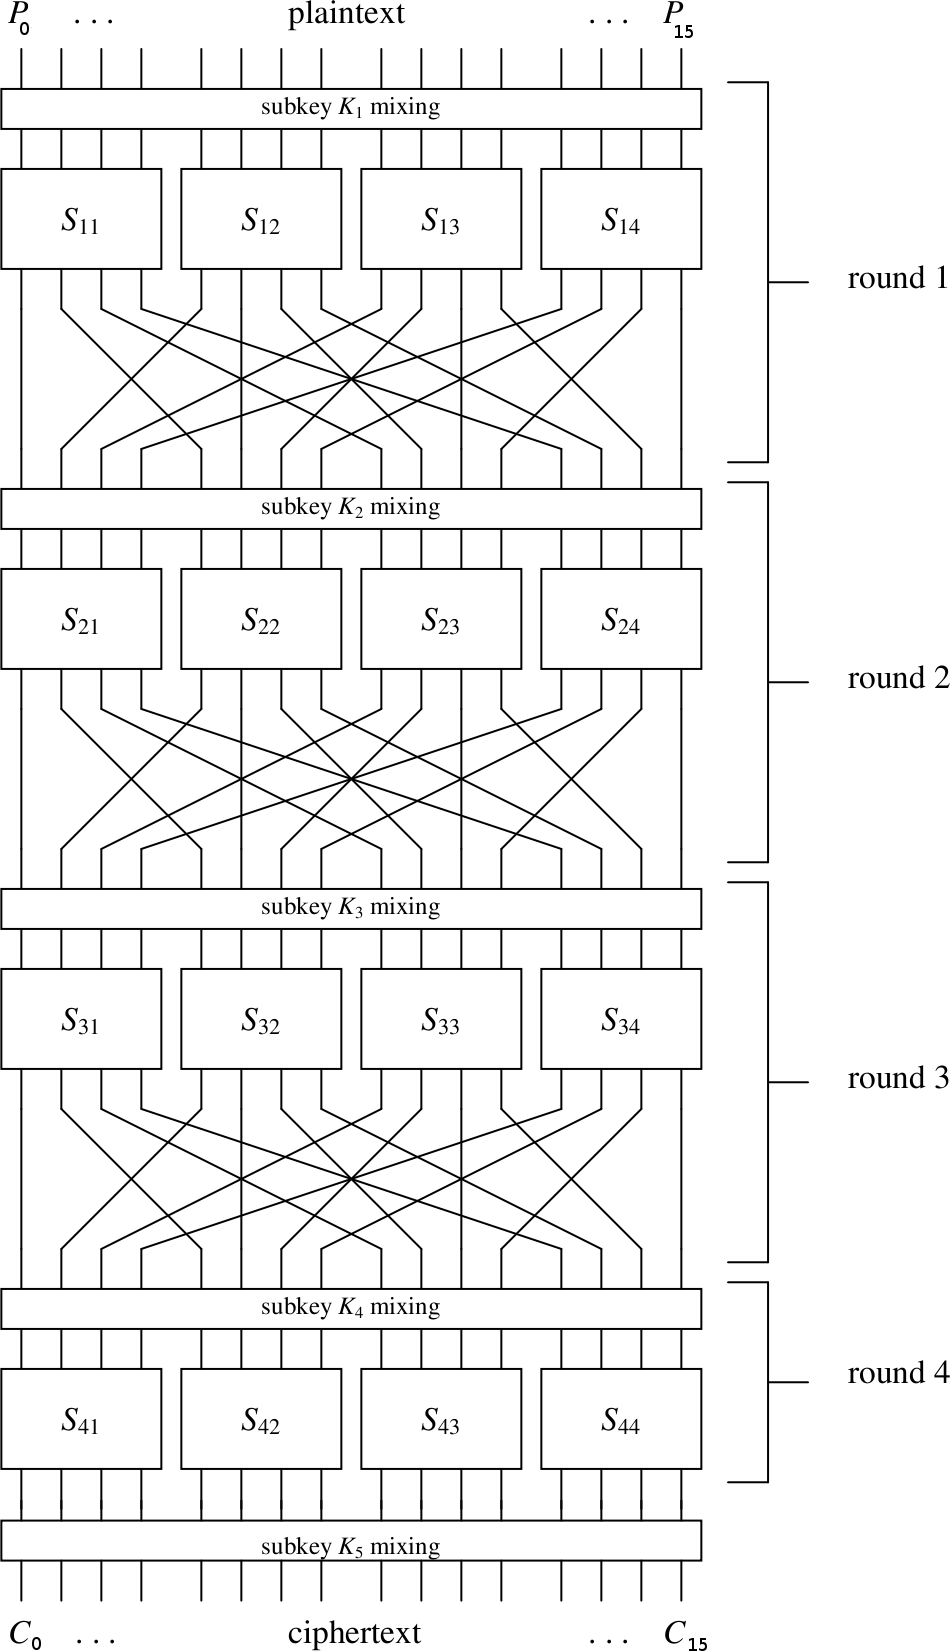
\includegraphics[height=0.6\textheight]{./heys-toy-cipher.png}
 \caption{Basic Structure of the Heys-Toy-Cipher from \cite{Heys2002}}
 \label{fig:htc}
\end{figure}


The cipher breaks the 16-bit data block into four 4-bit sub-blocks. Each sub-block forms an input to a $4\times4$ S-box (a substitution with 4 input and 4 output bits). The S-box is given by a lookup table where the most significant bit of the hexadecimal notation represents the leftmost bit of the S-box, i.e. we are using big endian notation.

\begin{center}
\begin{tabular}{|l |c|c|c|c| c|c|c|c| c|c|c|c| c|c|c|c|}
\hline
input  & 0 & 1 & 2 & 3 & 4 & 5 & 6 & 7 & 8 & 9 & A & B & C & D & E & F\\
\hline
output & E & 4 & D & 1 & 2 & F & B & 8 & 3 & A & 6 & C & 5 & 9 & 0 & 7\\
\hline
\end{tabular}
\end{center}

Alternatively, the S-box can be presented as polynomials in $\F_{2}[y_{3}, y_{2}, y_{1}, y_{0}, x_{3}, x_{2}, x_{1},
x_{0}]$ (where $x_3$ represents the least-significant input bit, $x_0$ the most-significant input bit, $y_3$ the
least-significant output bit and $y_0$ the most-significant output bit):

\begin{align*}
y_{0} =& x_{3}x_{2}x_{1} + x_{3} + x_{2} + x_{1} + x_{0} + 1,\\
y_{1} =& x_{3}x_{2}x_{0} + x_{3}x_{0} + x_{3} + x_{2}x_{1}x_{0} + x_{2}x_{0} + x_{1} + 1,\\
y_{2} =& x_{3}x_{1}x_{0} + x_{3}x_{0} + x_{2} + x_{1}x_{0} + x_{1} + 1,\\
y_{3} =& x_{3}x_{2}x_{1} + x_{3}x_{2} + x_{3}x_{1}x_{0} + x_{3}x_{0} + x_{3} + x_{2}x_{1} + x_{1}x_{0} + x_{1} + x_{0}.\\
\end{align*}

The permutation portion of a round is simply the transposition of the bits or the permutation of the bit positions. The permutation is given in the following table (where the numbers represent bit positions in the block, with 0 being the leftmost bit and 15 being the rightmost bit) and can be simply described as: the output $i$ of S-box $j$ is connected to input $j$ of S-box $i$. There would be no purpose for a permutation in the last round and, hence, the cipher does not have one. Please also note that the ordering here is little endian contrary to the big endian ordering of the S-box.

\begin{center}
\begin{tabular}{|l |c|c|c|c| c|c|c|c| c|c|c|c| c|c|c|c|}
\hline
  input  & 0 & 1 & 2 &  3 & 4 & 5 & 6 &  7 & 8 & 9 & 10 & 11 & 12 & 13 & 14 & 15 \\
\hline
output & 0 & 4 & 8 & 12 & 1 & 5 & 9 & 13 & 2 & 6 & 10 & 14 &  3 &  7 & 11 & 15 \\
\hline
\end{tabular}
\end{center}

Heys does not specify how subkeys are to be generated for the cipher so we use the identity map, i.e. each subkey is identically to the user-provided key. So the user-provided key  is added (XORed) to the output of the permutation layer and the result of this XOR is used as input for the next substitution layer.

One cipher round consists of an application of the substition layer, the permutation layer and the key addition. This is repeated four times as the cipher has four rounds. However, before the first round another key addition is performed and the fourth round does not feature a permutation.

We call $X_{i,j}$ the $j$-th bit/variable of the input of round $i$ and $Y_{i,j}$ the $j$-th output bit of the substition layer of the $i$-th round. We start counting the variables at $0$ and the rounds at $1$.


\subsection{An Equation System for the Heys-Toy-Cipher}

Constructing an equation system for the HTC is straight-forward once a polynomial representation of the S-box is found. Besides the S-box only the key addition needs to be accounted for and it is linear and thus easily represented as a set of polynomials.
                                                            
We represent the S-box by a set of 21 quadratic and 2 cubic polynomials, which form a \emph{degrevlex} Gröbner basis.

\begin{align*}
& x_{1}y_{0} + y_{3}y_{0} + y_{1}y_{0} + x_{1} + y_{3} + y_{1} + y_{0} + 1,\\
& x_{2}y_{0} + y_{2}y_{0} + y_{1}y_{0} + x_{2} + y_{2} + y_{1} + y_{0} + 1,\\
& x_{3}y_{0} + x_{0}y_{0} + y_{3}y_{0} + x_{2} + x_{1} + y_{3} + y_{2} + y_{0},\\
& x_{0}y_{1} + y_{3}y_{1} + y_{2}y_{1} + y_{1}y_{0} + x_{0} + y_{3} + y_{2} + y_{1} + y_{0} + 1,\\
& x_{1}y_{1} + y_{3}y_{1} + x_{0}y_{0} + y_{2}y_{0} + x_{2} + y_{2} + y_{1} + 1,\\
& x_{2}y_{1} + y_{2}y_{1} + y_{1}y_{0},\\
& x_{3}y_{1} + y_{3}y_{1} + y_{2}y_{1} + y_{1},\\
& y_{3}y_{2} + y_{2}y_{1} + x_{3} + x_{2} + x_{0} + y_{1},\\
& x_{0}y_{2} + y_{2}y_{0} + x_{3} + x_{2} + y_{3} + y_{2} + y_{0} + 1,\\
& x_{2}y_{2} + y_{2}y_{1} + x_{0}y_{0} + y_{1}y_{0} + x_{1} + y_{3} + y_{1} + 1,\\
& x_{3}y_{2} + x_{0}y_{0} + y_{2}y_{0} + y_{1}y_{0} + x_{1} + x_{0} + y_{2} + y_{0},\\
& x_{0}y_{3} + y_{3}y_{1} + y_{2}y_{1} + y_{3}y_{0} + x_{3} + x_{2} + y_{3} + y_{2} + y_{0} + 1,\\
& x_{1}y_{3} + y_{3}y_{1} + x_{0}y_{0} + y_{2}y_{0} + y_{1}y_{0},\\
& x_{2}y_{3} + y_{3}y_{1} + y_{2}y_{1} + y_{3}y_{0} + x_{3} + x_{2} + x_{0} + y_{3} + y_{1},\\
& x_{3}y_{3} + y_{3}y_{1} + y_{2}y_{1} + x_{3} + x_{2} + x_{0} + y_{3} + y_{1},\\
& x_{1}x_{0} + x_{1}y_{2} + y_{3}y_{0} + x_{2} + x_{0} + y_{1} + 1,\\
& x_{2}x_{0} + y_{3}y_{1} + y_{2}y_{1} + x_{3} + x_{2} + x_{1} + y_{3} + 1,\\
& x_{3}x_{0} + y_{3}y_{0} + y_{2}y_{0} + y_{1}y_{0} + x_{0} + y_{3} + y_{2} + y_{1} + y_{0} + 1,\\
& x_{2}x_{1} + x_{1}y_{2} + y_{3}y_{1} + y_{3}y_{0} + x_{1},\\
& x_{3}x_{1} + x_{1}y_{2} + y_{1}y_{0} + x_{3} + x_{2} + y_{3} + 1,\\
& x_{3}x_{2} + y_{3}y_{1} + y_{2}y_{1} + y_{3}y_{0} + y_{2}y_{0} + y_{1}y_{0} + x_{3} + x_{0} + y_{3} + y_{2} + y_{0} + 1,\\
& y_{2}y_{1}y_{0} + x_{1}y_{2} + y_{2}y_{0} + x_{3} + x_{2} + x_{0} + y_{2} + y_{1},\\
& y_{3}y_{1}y_{0} + y_{3}y_{0} + y_{1}y_{0} + x_{2} + y_{2} + y_{1} + 1.\\
\end{align*}

A HTC instance with $N_r$ rounds thus has $(N_r + 1) \cdot 16$ linear equations for the key additions, $N_r \cdot 4
\cdot 21$ quadratic equations and $N_r \cdot 4 \cdot 2$ cubic equations. These equations are in $16 + 2 \cdot N_r \cdot
16$ variables. Thus a four-round standard instance gives rise to $448$ equations in $144$ variables. We also add the
field equations to the set of equation and thus end up with a system of $592$ equations in $144$ variables. A three
round variant gives rise to a system with $452$ equations in $112$ variables.

\subsection{Linear Approximations}
Using a linear approximation matrix (cf.~\cite{Heys2002}) the following probabilistic linear equations can be found for the S-box:

Four linear equations are true with probability $0.875$:
\begin{align*}
0 &= x_{3} + y_{3} + y_{2} + y_{1} & 0 &= x_{2} + y_{2} + y_{1} + y_{0} + 1,\\
0 &= x_{3} + x_{2} + y_{3} + y_{0} + 1 & 0 &= x_{0} + y_{3} + y_{2} + y_{1} + y_{0} + 1.\\
\end{align*}

24 linear equations are true with probability $0.75$:
\begin{align*}
0 &= x_{1} + y_{3} + y_{1} + 1, & 0 &= x_{1} + y_{3} + y_{1} + y_{0} + 1,\\
0 &= x_{3} + x_{1} + y_{2} + y_{1}, & 0 &= x_{3} + x_{1} + y_{2} + y_{0} + 1,\\
0 &= x_{2} + x_{1} + y_{3} + y_{2}, & 0 &= x_{2} + x_{1} + y_{3} + y_{2} + y_{0},\\
0 &= x_{3} + x_{2} + x_{1} + y_{3} + y_{1} + 1, & 0 &= x_{3} + x_{2} + x_{1} + y_{1} + y_{0},\\
0 &= x_{3} + x_{0} + y_{0} + 1, & 0 &= x_{3} + x_{0} + y_{3} + y_{1} + y_{0},\\
0 &= x_{2} + x_{0} + y_{3}, & 0 &= x_{2} + x_{0} + y_{1} + 1,\\
0 &= x_{3} + x_{2} + x_{0} + y_{3}, & 0 &= x_{3} + x_{2} + x_{0} + y_{3} + y_{2} + 1,\\
0 &= x_{3} + x_{2} + x_{0} + y_{1}, & 0 &= x_{3} + x_{2} + x_{0} + y_{2} + y_{1},\\
0 &= x_{1} + x_{0} + y_{2}, & 0 &= x_{1} + x_{0} + y_{3} + y_{2} + y_{0},\\
0 &= x_{3} + x_{1} + x_{0} + y_{3} + y_{1}, & 0 &= x_{3} + x_{1} + x_{0} + y_{0} + 1,\\
0 &= x_{2} + x_{1} + x_{0} + y_{3} + y_{1} + 1, & 0 &= x_{2} + x_{1} + x_{0} + y_{1} + y_{0} + 1,\\
0 &= x_{3} + x_{2} + x_{1} + x_{0} + y_{2} + 1, & 0 &= x_{3} + x_{2} + x_{1} + x_{0} + y_{2} + y_{0}.
\end{align*}


\section{Linear Cryptanalysis in Algebraic Terms}
First, consider Matsui's \emph{Algorithm 1}. Essentially, a very simple probabilistic linear equation system is solved by evaluating it at enough data points. That is we compute $N$ varieties and check where they intersect most\footnote{Without lost of generality we may assume that we are looking for the point where they intersect most as we can simply add $1$ to one side of an equations.}. This intersection check is performed by incrementing counters for the respective varieties. 

Now, consider \emph{Algorithm 2}. In this variant a probabilistic linear relationship of the last round is replaced by a higher-order relationship true with probability $1$, while the probabilistic relations from the previous rounds remain. As a result more key bit information is available and only $R-1$ approximations are necessary. The 2R variant does the same for the first and the last round of the cipher. The cost of this transition however is that a more difficult systems have to be solved. In Matsui's paper and in linear cryptanalysis in general these systems are solved using brute force by trying all possible candidate keys. This is a reasonable approach because the search space is small.

Later, Knudsen and Robshaw \cite{Knudsen1996} pushed this idea further by explicitly adding probabilistic non-linear equations to the system. The advantage of this idea is that these might have higher probability than linear approximations but lower degree and fewer variables than the correct relationships. However, this approach poses a problem. Non-linear equations are not as easily XORed as linear equations in the sense that intermediate variables cancel out. Thus, it is more difficult to apply the \emph{Piling-Up} lemma (cf.~\cite{Heys2002}). Therefore \cite{Knudsen1996} restricts non-linear approximations to the outer rounds.

In algebraic cryptanalysis on the other hand the attacker considers polynomial systems which are always correct and tries to solve them using sophisticated means. However, as systems in linear cryptanalysis became more sophisticated researchers in algebraic cryptanalysis simplified their systems in order to gain better attacks. Examples of this trend are guessed key bits and BES-style equation systems for the AES \cite{murphy-robshaw:crypto2002} where the relationship $y = x^{254}$ is represented as $1 = xy$ which holds with probability $\frac{255}{256}$.

We can parameterise both attacks as follows: Let $F$ be a (potentially linear) polynomial system of equations, let $e$ be an estimation of the complexity of solving $F$, let $p$ be the probability an instance of $F$ is correct and $N$ the number of required (chosen or known) plaintext-ciphertext pairs. 

\begin{table}[htbp]
\begin{center}
\begin{tabular}{|l|c|c|c|}
\hline
Attack & $e$ & $p$ & $N$\\
\hline
Algebraic & $\ord{2^n}$ & $\approx 1$ & $\ord{1}$\\
Linear & $\ord{1}$ & $0 < p\neq 1/2 < 1$ & $\ord{1/|p -1/2|^2}$\\
\hline
\end{tabular}
\end{center}
\caption{Algebraic and linear attacks in comparison for an $n$-bit key.}
\label{tab:linalg-comp}
\end{table}

Thus, by increasing $N$ we can decrease $e$ (and vice versa) and we are faced with the optimisation problem where we modify different parameters in order to get an efficient attack. However, we need to translate linear cryptanalysis to algebraic terms first to show that such a balanced algorithm exists.

\subsection{Linear Cryptanalysis as an Algebraic Attack}
Consider Heys' Toy Cipher and a 1R linear cryptanalysis. First, a linear approximation of the first three rounds needs to
be found. \cite{Heys2002} uses four linear equations which are true with probability $<1$ to mount a linear cryptanalysis. These are:
\begin{align*}
0 &= Y_{1, 5} + X_{1, 4} + X_{1, 6} + X_{1,7}\\
0 &= Y_{2, 5} + Y_{2, 7} + X_{2, 5} + 1 \\
0 &= Y_{3, 5} + Y_{3, 7} + X_{3, 5} + 1 \\
0 &= Y_{3,13} + Y_{3,15} + X_{3,13} + 1 \\ 
\end{align*}

We added $1$ to those equations which are true with a negative bias to make sure they have a positive bias.
Each of those is true with $p=0.75$ and consequently they are all true with probability $0.75^{4} \simeq  0.32$ under the assumption they are independent. By using the Piling-Up Lemma (cf.~\cite{Matsui1993}, \cite{Heys2002}) the
sum 
\[
X_{4,5} + X_{4,7} + X_{4,13} + X_{4,15} +  P_{4} + P_{6} + P_{7} + K_{4} + K_{15} + 1
\]
of the right hand sides of these equations and the intermediate linear polynomials is equal to zero with probability
$0.53125$.

As this is a relationship between some plaintext bits and some bits from the input of the fourth round ($X_{4,j}$) which holds with a certain bias -- subject to the sum of $K_{4}$ and $K_{15}$ -- \emph{Algorithm 2} proceeds by trying all candidate keys ($K_{4}$, $K_{5}$, $K_{6}$, $K_{7}$, $K_{12}$, $K_{13}$, $K_{14}$, $K_{15}$) to decrypt the known ciphertext. If $X_{4,5} + X_{4,7} + X_{4,13} + X_{4,15}$ matches $P_{4} + P_{6} + P_{7}  + K_{4} + K_{15} + 1$ a counter for the used candidate key is incremented. If this is done often enough, we expect to see a peak for the correct candidate key.                                                                                                                                                                                                                                                                                                                                                                    

To replicate the same using Gröbner basis algorithms we simply add our equations for the two missing S-boxes and the final key addition. We call the resulting system $F$. If we subsitute the candidate keys in $F$ and compute a Gröbner basis we can check if the equation system is satisfiable, i.e. the Gröbner basis $\neq \{1\}$. If the Gröbner basis is $\neq \{1\}$ we increment a count for the considered candidate key and proceed. Otherwise, we do not increment the counter. We can avoid the candidate key substitution step by studying the symbolic Gröbner basis and incrementing a counter for each solution restricted to $K_{4}$, $K_{5}$, $K_{6}$, $K_{7}$, $K_{12}$, $K_{13}$, $K_{14}$, $K_{15}$.

The equation system we attempt to solve in this case is given 
\begin{enumerate} 
 \item by the linear approximation
\begin{align*}
0 =& X_{4,5} + X_{4,7} + X_{4,13} + X_{4,15} + K_{4} + K_{15} + P_5 + P_7 + P_8,\\
\end{align*}
\item the S-Box equations for the last round and
\begin{align*}
0 =& X_{4,4}X_{4,5}X_{4,6} + X_{4,4} + X_{4,5} + X_{4,6} + X_{4,7} + Y_{4,7} + 1, \\
0 =& X_{4,4}X_{4,5}X_{4,7} + X_{4,4}X_{4,7} + X_{4,4} + X_{4,5}X_{4,6}X_{4,7} + X_{4,5}X_{4,7} + X_{4,6} + Y_{4,6} + 1, \\
0 =& X_{4,4}X_{4,6}X_{4,7} + X_{4,4}X_{4,7} + X_{4,5} + X_{4,6}X_{4,7} + X_{4,6} + Y_{4,5} + 1, \\
0 =& X_{4,4}X_{4,5}X_{4,6} + X_{4,4}X_{4,5} + X_{4,4}X_{4,6}X_{4,7} + X_{4,4}X_{4,7} + X_{4,4}  \\
&  + X_{4,5}X_{4,6} + X_{4,6}X_{4,7} + X_{4,6} + X_{4,7} + Y_{4,4}, \\
\\
0 =& X_{4,12}X_{4,13}X_{4,14} + X_{4,12} + X_{4,13} + X_{4,14} + X_{4,15} + Y_{4,15} + 1, \\
0 =& X_{4,12}X_{4,13}X_{4,15} + X_{4,12}X_{4,15} + X_{4,12} + X_{4,13}X_{4,14}X_{4,15} + X_{4,13}X_{4,15} + X_{4,14} + Y_{0414} + 1, \\
0 =& X_{4,12}X_{4,14}X_{4,15} + X_{4,12}X_{4,15} + X_{4,13} + X_{0414}X_{0415} + X_{4,14} + Y_{4,13} + 1, \\
0 =& X_{4,12}X_{4,13}X_{4,14} + X_{4,12}X_{4,13} + X_{4,12}X_{4,14}X_{4,15} + X_{4,12}X_{4,15} \\
& + X_{4,12}  + X_{4,13}X_{4,14} + X_{4,14}X_{4,15} + X_{4,14} + X_{4,15} + Y_{4,12}, \\
\end{align*}
\item the final key addition
\begin{align*}
0 =& Y_{4,4} + K_{4} + C_4, & 0 =& Y_{4,5} + K_{5} + C_5, & 0 =& Y_{4,6} + K_{6} + C_6, & 0 =& Y_{4,7} + K_{7} + C_7,\\
0 =& Y_{4,12} + K_{12} + C_{12}, & 0 =& Y_{4,13} + K_{13} + C_{13}, & 0 =& Y_{4,14} + K_{14} + C_{14}, & 0 =& Y_{4,15} +
K_{15} + C_{15}.\\
\end{align*}
\end{enumerate}
We also add some field equations to restrict the variety to the base field.

The attacker now can increase $e$ as introduced before by setting up a more complicated equation system. For example
this 1R attack can be extended to a 2R attack by replacing the linear approximation of
first round S-Box with the correct cubic equation. Furthermore, we may want to insert the correct equations
for the S-Box in the second round. As $Y_{2,5}$ depends on all of $X_{2,4} \dots X_{2,7}$ this implies inserting
the correct cubic equations for $Y_{1,1}$,$Y_{1,5}$,$Y_{1,9}$,$Y_{1,13}$ as well. If we continue this
approach up to the penultimate round we end up with the full correct equation system.

Thus by adding more correct equations we increase $e$ but decrease $N$ and increase $p$. An alternative approach is not
to \emph{replace} linear approximations but still to \emph{add} correct equations.

\subsection{Enhancing Algebraic Attacks with Linear Cryptanalysis}

The standard strategy for simplifying an equation system in algebraic cryptanalysis is to guess key bits. The time saved during a single Gröbner basis or similar 
calculation is -- up to some number of guesses $g$ -- much greater than the addition time that is required -- by guessing $2^{g}$ times.

However, using the linear approximations arising from linear cryptanalysis we might able to do better: Guessing a linear eqution that holds with probability $p > 0.5$ is better than guessing a relationship between key variables and values which holds with probability $p = 0.5$.

\subsubsection{Experiments with Toy Instances}
\label{sec:experiments}
All experiments were carried out using the computer algebra system \Sage 2.7 \cite{sage} and the $F_4$ algorithm (cf.~Chapter~\ref{chapter:f4}) implemented in \Magma 2.13-5 \cite{magma}.

In the Tables~\ref{tab:exp-3-rounds} and \ref{tab:exp-4-rounds}, the symbol $\#$ represents the number of trials, $N_r$ represents the number of rounds, $b$ the bias of the approximations, $r$ the experimental success rate and $t$ the average time it took to compute a Gröbner basis. The estimated success rate (``est. $r$'') is computed by taking the probability of the approximates to the power of the number of the approximation, i.e. it estimates the success rate if those approximations are independent and if exactly one solution exists for the system. The quotient $t/r$ indicates the time it would take to attack the system using the given approximation.

All experiments were carried out on a 2.33~GHz Intel \CTD notebook with 2GB RAM unless stated otherwise. To carry out these experiments the number of rounds had to be reduced to $3$ in many cases because we ran out of RAM if 4 rounds were to be used without any approximations.

The polynomial ring used during all three-round experiments is

\begin{align*}
P = \F_{2}[&X_{1,0}, \dots, X_{1,15}, Y_{1,0}, \dots, Y_{1,15}, X_{2,0}, \dots, X_{2,15}, Y_{2,0}, \dots, Y_{2,15}, \\
&X_{3,0}, \dots, X_{3,15}, Y_{3,0}, \dots, Y_{3,15}, K_{0}, \dots, K_{15}].\\
\end{align*}

First, the time to compute a \emph{degrevlex} Gröbner basis without any approximations was recorded. It takes approximately 40 seconds on our system. Next, up to 5 key variables were guessed. We note that the actual success rate is always greater than the estimated success rates which can be accounted for by the fact that the system does not necessarily have only one solution.

Next, an approximation with a very high probability is chosen: $x_2 + x_3 + y_0 + y_3 + 1$ is true with probability $0.875$. Two S-Boxes per round were approximated using this linear polynomial and we see a successrate of over 50\%.

However, this approximation does not necessarily give better results than simply guessing key-bits. The next approach is to use the same linear approximation polynomials used in Heys'  linear cryptanalysis \cite{Heys2002}. Afterwards the sum -- i.e. a relationship between plaintext, ciphertext and some key bits -- as presented for linear cryptanalysis is used.

Finally, an approximation which we believed to be a ``good'' approximation is used. It is deemed ``good'' because it has high probability and is spread throughout the cipher. Indeed, it seems to provide the best results at 8.68 seconds of estimated attack time.

\begin{table}[ht]
\begin{small}
\begin{center}
\begin{tabular}{|c|r|l|c|c|c|r|r|}
\hline
\#	& $N_r$ & Approximations & $b$ & $r$ & est. $r$ & $t$ & $t$ / $r$\\
\hline

25 & 3 & -- & 0 & 1 & 1 & 40.64 & 40.64\\

\hline % guessed key bits

25 & 3 & $K_{0}$				& 0 & 0.64 & 0.5 & 30.40	 & 47.50\\
\hline
25 & 3 & $K_{0},K_{1}$			& 0 & 0.44 & 0.25 & 12.57 & 28.57\\
\hline
50 & 3 & $K_{0},K_{1},K_{2}$		& 0 & 0.28 & 0.13 & 4.74 & 16.93\\
\hline
50 & 3 & $K_{0},K_{1},K_{2},K_{3}$	& 0 & 0.16 & 0.06 & 2.46 & 15.38\\
\hline
50 & 3 & $K_{0},K_{1},K_{2},K_{3},K_{4}$	& 0 & 0.04 & 0.03 & 1.25 & 31.25\\

\hline % high probability approximation

50 & 3 &  $X_{1, 2} + X_{1, 3} + Y_{1, 0} + Y_{1, 3}$ + 1 & 0.38 & 0.58 & 0.45 & 12.77 & 22.02\\
   &   &  $X_{1,14} + X_{1,15} + Y_{1,12} + Y_{1,15}$ + 1 & & & & & \\
   &   &  $X_{2, 2} + X_{2, 3} + Y_{2, 0} + Y_{2, 3}$ + 1 & & & & & \\
   &   &  $X_{2,14} + X_{2,15} + Y_{2,12} + Y_{2,15}$ + 1 & & & & & \\
   &   &  $X_{3, 2} + X_{3, 3} + Y_{3, 0} + Y_{3, 3}$ + 1 & & & & & \\
   &   &  $X_{3,14} + X_{3,15} + Y_{3,12} + Y_{3,15}$ + 1 & & & & & \\

\hline   % linear cryptanalysis single

50 & 3 & $Y_{1, 5} + X_{1, 4} + X_{1, 6} + X_{1, 7}$ & 0.25 & 0.5 & 0.31 & 7.89 & 15.78\\
   &   & $Y_{2, 5} + Y_{2, 7} + X_{2, 5} + 1$ & & & & & \\
   &   & $Y_{3, 5} + Y_{3, 7} + X_{3, 5} + 1$ & & & & & \\
   &   & $Y_{3,13} + Y_{3,15} + X_{3,13} + 1$ & & & & & \\

\hline % linear cryptanalysis piling-up
25 & 3 & $K_{4} + K_{15} + P_{4} + P_{6} + P_{7} +$ & 0.53 & 0.64 & 0.53 & 28.58 & 44.65\\
   &   & $C_{5} + C_{7} + C_{13} + C_{15} + 1$ & & & & & \\

\hline % good approximation

50 & 3 & $X_{1, 0} + X_{1, 3} + Y_{1, 0} + 1$ & 0.25 & 0.16	& 0.08 & 1.64 &10.25\\
   &   & $X_{1, 4} + X_{1, 7} + Y_{1, 4} + 1$ & & & & & \\
   &   & $X_{1,12} + X_{1,15} + Y_{1,12} + 1$ & & & & & \\
   &   & $X_{2, 0} + X_{2, 3} + Y_{2, 0} + 1$ & & & & & \\
   &   & $X_{2, 4} + X_{2, 7} + Y_{2, 4} + 1$ & & & & & \\
   &   & $X_{2,12} + X_{2,15} + Y_{2,12} + 1$ & & & & & \\
   &   & $X_{3, 0} + X_{3, 3} + Y_{3, 0} + 1$ & & & & & \\
   &   & $X_{3, 4} + X_{3, 7} + Y_{3, 4} + 1$ & & & & & \\
   &   & $X_{3,12} + X_{3,15} + Y_{3,12} + 1$ & & & & & \\

\hline

50 & 3 & $X_{1, 0} + X_{1, 3} + Y_{1, 0} + 1$ & 0.25 & 0.4 & 0.18 & 3.47 &8.68\\
   &   & $X_{1,12} + X_{1,15} + Y_{1,12} + 1$ & & & & & \\
   &   & $X_{2, 0} + X_{2, 3} + Y_{2, 0} + 1$ & & & & & \\
   &   & $X_{2,12} + X_{2,15} + Y_{2,12} + 1$ & & & & & \\
   &   & $X_{3, 0} + X_{3, 3} + Y_{3, 0} + 1$ & & & & & \\
   &   & $X_{3,12} + X_{3,15} + Y_{3,12} + 1$ & & & & & \\

\hline

50 & 3 & $X_{1, 0} + X_{1, 3} + Y_{1, 0} + 1$ & 0.25 & 0.56 & 0.31 & 6.42 & 11.46\\
   &   & $X_{1,12} + X_{1,15} + Y_{1,12} + 1$ & & & & & \\
   &   & $X_{2, 0} + X_{2, 3} + Y_{2, 0} + 1$ & & & & & \\
   &   & $X_{2,12} + X_{2,15} + Y_{2,12} + 1$ & & & & & \\

\hline

25 & 3 & $X_{1, 0} + X_{1, 3} + Y_{1, 0} + 1$ & 0.25 & 0.84 & 0.56 & 17.28 & 20.57\\
   &   & $X_{1,12} + X_{1,15} + Y_{1,12} + 1$ & & & & & \\

\hline
\end{tabular}
\end{center}
\end{small}
\caption{Experimental results for three rounds of HTC.}
\label{tab:exp-3-rounds}
\end{table}

Table~\ref{tab:exp-4-rounds} mounts the best attack from the 3-round cipher against a 4-round cipher. We end up with
an estimated attack time of roughly 200 seconds.

\begin{table}[ht]
\begin{small}
\begin{center}
\begin{tabular}{|c|r|c|c|c|c|r|r|}
\hline
\#	& $N_r$ & Approximations & $b$ & $r$ & est. $r$ & $t$ & $t$ / $r$\\
\hline
50 & 4 & $X_{1, 0} + X_{1, 3} + Y_{1, 0} + 1$ & 0.25 & 0.26 & 0.1 & 50.9 & 195.77\\
   &   & $X_{1,12} + X_{1,15} + Y_{1,12} + 1$ & & & & & \\
   &   & $X_{2, 0} + X_{2, 3} + Y_{2, 0} + 1$ & & & & & \\
   &   & $X_{2,12} + X_{2,15} + Y_{2,12} + 1$ & & & & & \\
   &   & $X_{3, 0} + X_{3, 3} + Y_{3, 0} + 1$ & & & & & \\
   &   & $X_{3,12} + X_{3,15} + Y_{3,12} + 1$ & & & & & \\
   &   & $X_{4, 0} + X_{4, 3} + Y_{4, 0} + 1$ & & & & & \\
   &   & $X_{4,12} + X_{4,15} + Y_{4,12} + 1$ & & & & & \\
\hline
50 & 4 & $X_{1, 0} + X_{1, 3} + Y_{1, 0} + 1$ & 0.25 & 0.22 & 0.18 &118.0	& 536.36\\
   &   & $X_{1,12} + X_{1,15} + Y_{1,12} + 1$ & & & & & \\
   &   & $X_{2, 0} + X_{2, 3} + Y_{2, 0} + 1$ & & & & & \\
   &   & $X_{2,12} + X_{2,15} + Y_{2,12} + 1$ & & & & & \\
   &   & $X_{3, 0} + X_{3, 3} + Y_{3, 0} + 1$ & & & & & \\
   &   & $X_{3,12} + X_{3,15} + Y_{3,12} + 1$ & & & & & \\
\hline
\end{tabular}
\end{center}
\end{small}
\caption{Experimental results for four rounds of HTC.}
\label{tab:exp-4-rounds}
\end{table}

We also computed a \emph{degrevlex} Gröbner basis for a full four-round HTC instance on William Stein's old \url{sage.math.washington.edu} machine\footnote{purchased National Science Foundation under Grant No. 0555776} which has 64GB RAM and 16 1.8~Ghz \Opteron processors. It took 55049s (= 15.3h) cputime to compute this Gröbner basis while -- for comparison -- it took 60s cputime to compute a Gröbner basis for a three round cipher. The three round computation takes approximately 40s on the 2.33~Ghz \CTD machine.

\section{Final Remarks}
Of course, all these ``attacks'' are ridiculously inefficient when compared to a simple linear cryptanalysis or even a brute force attack. However, they do demonstrate the point that considering linear approximations may be beneficial when compared to simply guessing key bits in algebraic cryptanalysis.

\chapter{Algebraic Techniques in Differential Cryptanalysis}
\label{chapter:algebraic_differential_cryptanalysis}
Besides linear cryptanalysis, differential cryptanalysis is probably the most established cryptanalytic method against block ciphers~\cite{des-dc}. In this chapter we combine algebraic techniques with differential cryptanalysis to various novel algorithms. We also show the viability of our new methods by applying them to reduced variants of the block ciphers \PRESENT and KTANTAN32.

This chapter consists of a revised, updated and extended version of the paper titled ``Algebraic Techniques in Differential Cryptanalysis'' by Carlos Cid and the author presented at FSE 2009 \cite{adc:fse2009}. Some results were also published in the paper ``Algebraic Precomputations in Differential and Integral Cryptanalysis'' by Carlos Cid, Thomas Dullien, Jean-Charles Faugère, Ludovic Perret and the author \cite{acdfp:inscrypt2010}. Furthermore, some results in this chapter were also presented at the Tools for Cryptanalysis 2010 workshop. The experimental results against KTANTAN32 are unpublished but were partly presented at the rump session of the Early Symmetric Cryptography Seminar 2010 in Remich, Luxembourg. The later results were obtained while visiting the group of Jean-Charles Faugère in Paris in 2009.

This chapter is structured as follows. First, we briefly describe differential cryptanalysis and give the basic idea of the attack in Section~\ref{sec:overview}. We then describe the block cipher \PRESENT in Section~\ref{sec:present} and existing attacks against a reduced round versions of \PRESENT. In Section~\ref{sec:ktantan32} we describe the block cipher KTANTAN32. In Section~\ref{sec:adc} we describe the application of our new attack technique against reduced round versions of \PRESENT and KTANTAN32. We present a brief discussion of the attacks and possible extensions in Section~\ref{sec:discussion}.


\section{Overview of the New Attack Technique}
\label{sec:overview}
Since our approach combines differential and algebraic cryptanalysis, we briefly describe differential cryptanalysis below. Algebraic cryptanalysis was discussed in Chapter~\ref{chapter:algebraic_attacks}.

\subsection{Differential Cryptanalysis}
Differential cryptanalysis was formally introduced by Biham and Shamir at Crypto'90 \cite{Biham1991}, and has since been successfully used to attack a
wide range of block ciphers. In its basic form, the attack can be used to distinguish a $n$-bit block cipher from a random permutation. By considering the distribution of output \emph{differences} for the non-linear components of the cipher (e.g. the S-Box), the attacker may be able to construct \emph{differential characteristics} \mbox{$P' \oplus P'' = \Delta P \rightarrow \Delta C = C' \oplus C''$} for a number of rounds $N$ that are valid with probability $p$. If $p \gg 2^{-n}$, then by querying the cipher with a large number of plaintext pairs with prescribed difference $\Delta P$, the attacker may be able to distinguish the cipher by counting the number of pairs with the output difference predicted by the characteristic. A pair for which the characteristic holds is called a \emph{right pair}. A pair which is not a right pair is a \emph{wrong pair}.

By modifying the attack, one can use it to recover key information. Instead of characteristics for the full $N$-round cipher, the attacker considers characteristics valid for $r$ rounds only ($r = N - R $, with $R>0$). If such characteristics exist with non-negligible probability the attacker can guess some key bits of the last rounds, partially decrypt the known ciphertexts, and verify if the result matches the one predicted by the characteristic. Candidate (last round) keys are counted, and as random noise is expected for wrong key guesses, eventually a peak may be observed in the candidate key counters, pointing to the correct round key\footnote{In some variants, as described in \cite{fulldes-dc}, no candidate key counters are required; see Section~\ref{sec:discussion} for a brief discussion of this attack.}.

Note that due to its statistical nature, differential cryptanalysis requires a very large number of plaintext-ciphertext pairs (for instance, approximately $2^{47}$ chosen plaintext pairs are required to break DES \cite{fulldes-dc}). Many extensions and variants of differential cryptanalysis exist, such as the Boo\-merang attack \cite{Wagner1999} and truncated and higher-order differentials \cite{Knudsen1995}. The technique is however very well understood, and most modern ciphers are designed to resist to differential cryptanalysis. This is often achieved by carefully selecting the cipher's non-linear operations and diffusion layer to make sure that if such differential characteristics exist, then $r \ll N$ which ensures that backward key guessing is impractical. The AES is a prime example of this approach~\cite{Daemen2002}.

\subsection{Algebraic Techniques in Differential Cryptanalysis}

A first idea in extending algebraic cryptanalysis is to use more plain\-text--cipher\-text pairs to construct the equation system. Given two equation systems $F'$ and $F''$ for two plaintext--ciphertext pairs $(P',C')$ and $(P'',C'')$ under the same encryption key $K$, we can combine these equation systems to form a system $F = F' \cup F''$. Note that while $F'$ and $F''$ share the key and key schedule variables, they do not share most of the state variables. Thus the cryptanalyst gathers almost twice as many equations, involving however many new variables. Experimental evidence indicates that this technique may often help in solving a system of equations at least up to a certain number of rounds~\cite{faugere:fse2007,bulgin-brickenstein:eprint2008}. The second step is to consider probabilistic relations that may arise from differential cryptanalysis, giving rise to what we call \emph{Attack-A}.

\subsubsection{\emph{Attack-A}.}

For the sake of simplicity, we assume the cipher is an Substitution-Permutation-Network (SP-net\-work), which iterates layers of non-linear transformations (e.g. S-Box operations) and affine transformations. Now consider a differential characteristic $\Delta = (\delta_0, \delta_1, \ldots , \delta_r)$ for a number of rounds, where $\delta_{i-1} \rightarrow \delta_{i}$ is a one-round difference arising from round $i$ and valid with probability $p_{i}$. If we assume statistical independence of one-round differences, the characteristic $\Delta$ is valid with probability $p = \prod p_i$. Each one-round difference gives rise to equations relating the input and output pairs for active S-Boxes. Let $X'_{i,j}$ and $X''_{i,j}$ denote the $j$-th bit of the input to the S-Box layer in round $i$ for the systems $F'$ and $F''$, respectively. Similarly, let $Y'_{i,j}$ and $Y''_{i,j}$ denote the corresponding output bits. Then we have that the expressions
$$
X'_{i,j} + X''_{i,j} = \Delta X_{i,j} \rightarrow \Delta Y_{i,j} = Y'_{i,j} + Y''_{i,j},
$$
where $\Delta X_{i,j}, \Delta Y_{i,j}$ are known values predicted by the characteristic, are valid with some non-neg\-ligible probability $q$ for bits of active S-Boxes. Similarly, for non-active S-Boxes (that are not involved in the characteristic $\Delta$ and therefore have input/output difference zero), we have the relations
$$
X'_{i,j} + X''_{i,j} = 0 = Y'_{i,j} + Y''_{i,j}
$$
also valid with a non-negligible probability.

If we consider the equation system $F = F' \cup F''$, we can combine $F$ and all such linear relations arising from the characteristic $\Delta$. This gives rise to an equation system $\overline{F}$ which holds with probability $p$. If we attempt to solve such a system for approximately $1/p$ pairs of plaintext--ciphertext, we expect at least one non-empty solution, which should yield the encryption key. For a full algebraic key recover we expect the system $\overline{F}$ to be easier to solve than the system $F = F' \cup F''$, because many linear constraints were added without adding any new variables. However, we do not know \emph{a priori} how difficult it will be to solve the system approximately $1/p$ times. Yet, this system $\overline{F}$ may be used to recover some key information, leading to an attack we call \emph{Attack-B}.

\subsubsection{\emph{Attack-B}.}
Now, assume that we have an SP-network, a differential characteristic $\Delta = (\delta_0, \delta_1, \ldots , \delta_r)$ valid for $r$ rounds with probability $p$, and $(P',P'')$ a right pair for $\Delta$ (so that $\delta_0 = P' \oplus P''$ and $\delta_r$ holds for the output of round $r$). For simplicity, let us assume that only one S-Box is active in round 1, with input $X_{1,j}'$ and $X_{1,j}''$ (restricted to this S-Box) for the plaintext $P'$ and $P''$ respectively, and that there is a key addition immediately before the S-Box operation, that is $$S(P_j' \oplus K_{0,j}) = S(X_{1,j}') = Y_{1,j}' \ \textrm{and} \ S(P_j'' \oplus K_{0,j}) = S(X_{1,j}'') = Y_{1,j}''.$$ The S-Box operation $S$ can be described by a (vectorial) Boolean function, expressing each bit of the output $Y_{1,j}'$ as a polynomial function (over $\field{F}_2$) on the input bits of $X_{1,j}'$ and $K_{0,j}$. If $(P',P'')$ is a right pair, then the polynomial equations arising from the relation $$\Delta Y_{1,j}= Y_{1,j}' \oplus Y_{1,j}'' = S(P_j' \oplus K_{0,j}) \oplus S(P_j'' \oplus K_{0,j})$$ give us a very simple equation system to solve, with only the key variables $K_{0,j}$ as unknowns. These equations do not vanish identically because we are considering non-zero differences. This is a consequence of the simple Lemma below:
\begin{lemma}
\label{lem:sbox-prob}
Given a differential $\Delta$ with a first round active S-Box with a difference that is true with probability $2^{-b}$, then from a right pair we can recover $b$ bits of information about the key from this S-Box.
\end{lemma}
Consequently, if we had an effective distinguisher to determine whether $\Delta Y_{1,j}$ holds, we could learn some bits of information about the round keys involved in the first round active S-Boxes.

Experimentally, we found that, for some ciphers and up to a number of rounds, \emph{Attack-A} can be used as such a distinguisher. More specifically, we
noticed that finding a contradiction (i.e. the Gr\"obner basis equal to $\{1\}$) was much faster than computing the full solution of the system if the system was consistent (that is, when we have a right pair).  Thus, rather than fully solving the systems to eventually recover the secret key as suggested in \emph{Attack-A}, the \emph{Attack-B} proceeds by measuring the time $t$ it maximally takes to find that the system is inconsistent\footnote{Other features of the calculation -- like the size of the intermediate matrices created by $F_4$ -- may also be used instead of the time $t$.}, and assume we have a right pair with good probability if this time $t$ elapsed without a contradiction. In particular, we expect $\Delta Y_{1,j}$ to hold with good probability. Thus, we want the probability that $\Delta Y_{1,j}$ holds to be close to $1$ if the time $t$ elapsed without \emph{Attack-A} finding a contradiction. It follows from Lemma~\ref{lem:sbox-prob} that this allows to recover information about the key. One needs to be able to experimentally estimate the time $t$, but for some ciphers this appears to be an efficient form of attack.

An alternative form of \emph{Attack-B} is to recover key bits from the last round. Assume that the time $t$ passed for a pair ($P'$,$P''$), i.e. that we probably found a right pair. Now, if we guess and fix some subkey bits in the last rounds, we can check whether the time $t$ still passes without a contradiction. If this happens, we assume that we guessed correctly. However, for this approach to work we need to guess enough subkey bits to detect a
contradiction quickly. An obvious choice is to guess all subkey bits involved in the last round, which effectively removes one round from the system.

\subsubsection{\emph{Generalised Attack-B}.}

There is no \emph{a priori} reason to restrict the argument for \emph{Attack-B} to the first round.

Let $\Delta$, $r$, $P'$, $P''$ be as before. Set up two equation systems $F'$ and $F''$ involving $P',C'$ and $P'',C''$ respectively and discard any polynomials from the rounds greater than $s$ where $s$ is a small integer larger than $0$. Previously we had $s=1$. We add linear equations as suggested by the characteristic and use this system to recover information about the key from the first $s$ rounds.

In order to avoid the potentially costly Gröbner basis computation for every candidate pair replace the tuples of constants $P'$ and $P''$ by tuples of symbols. Now, following the discussion in Chapter~\ref{chapter:algebraic_features} we can compute polynomials involving only key variables and the newly introduced plaintext variables $P'$ and $P''$. Assume that we can indeed compute the Gröbner basis with $P'$ and $P''$ symbols for the first $s$ rounds and the linear equations arising from the characteristic added. Assume further that the probability that the characteristic restricted to $s$ rounds holds is $2^{-b}$ and that we computed $m_s$ polynomials in the variables $K_0$, $P'$ and $P''$. This means that we recover $b$ bits of information (cf. Section~\ref{sec:discussion}) when we evaluate all $m_s$ polynomials such that we replace $P'$ and $P''$ by their actual values.

\subsubsection{\emph{Attack-C}.}

Experimental evidence with \PRESENT (cf. Section~\ref{sec:adc}) indicates that the bulk of the running time of \emph{Attack-B} mainly relies on the differential $\delta_0 \rightarrow \delta_r$ rather than the characteristic $\Delta$ when finding contradictions in the systems. The runtimes for finding contradictions for $N=17$ and differential characteristic of length $r=14$ did not differ significantly from the runtimes for the same task with $N=4$ and $r=1$ (cf. Table~\ref{tab:present-att-b}). This indicates that the computational difficulty is mostly determined by the difference $R = N-r$, the number of ``free'' rounds. We thus define a new attack (\emph{Attack-C}) where we remove the equations for rounds $\leq r$. 

This significantly reduces the number of equations and variables. After these equations are removed we are left with $R$ rounds for each plaintext--ciphertext pair to consider; these are related  by the output difference predicted by the differential. As a result, the algebraic computation is essentially equivalent to solving a related cipher of $2R-1$ rounds (from $C'$ to $C''$ via the predicted difference $\delta_r$) using an algebraic meet-in-the-middle attack~\cite{alg-aes-book}. This ``cipher'' has a symmetric key schedule and only $2R-1$ rounds rather than $2R$ since the S-Box applications after the difference $\delta_r$ are directly connected and lack a key addition and diffusion layer application between them. Thus we can consider these two S-Box applications as one S-Box application of S-Boxes $S_{i}$ defined by the  known difference $\delta_r$: $S_{i}(x_{i,\dots,i+s}) = S(S^{-1}(x_{i,\dots,i+s}) + \delta_{r,(i,\dots,i+s)})$ for $i \in \{0,s,2s,\dots,n\}$ and $s$ the size of the S-Box. The basic idea of how the equation system is constructed is depicted in Figure~\ref{fig:attack-c}.

\begin{figure}[h]
 \centering
 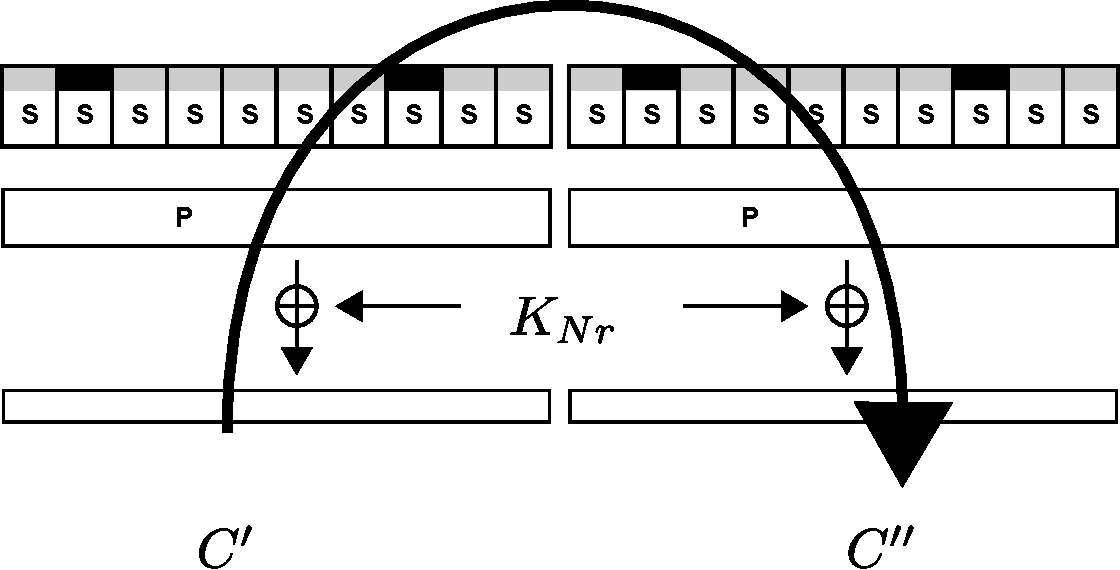
\includegraphics[width=.6\textwidth]{./attack-c.pdf}
 \caption{\emph{Attack-C} style equation system}
 \label{fig:attack-c}
\end{figure}


Again, we attempt to solve the system and wait for a fixed time $t$ to find a contradiction in the system. If no contradiction is found, we know that the pair $C',C''$ can be a right pair under some key. Thus we can consider \emph{Attack-C} as a quite expensive but thorough filter function: we invest more work in the management of the outer rounds using algebraic techniques.

Note that we cannot be certain about the output difference of the first round active S-Boxes or even that the differential $\delta_0 \rightarrow \delta_r$ holds. However, the attack can be adapted such that we can still recover key bits, for instance by considering multiple suggested right pairs. A second option is to attempt to solve the resulting smaller system to recover an encryption key candidate. Alternatively, we can execute the guess-and-verify step described above.

In order to gain more precise filters, we may add rounds prior to the round $r$ to our equation system. Instead of either stopping at round $r$ (counting from the rear) or going all the way as in \emph{Attack-B}, we may choose to add for example four more rounds prior to the round $r$. As Table~\ref{tab:present-bc} shows, this indeed improves the precision of the filter at the cost of being potentially more expensive.

\emph{Attack-C} has one caveat though. When we consider ciphers where the key-size is bigger than the block-size the solution space for the related ``cipher'' is significantly larger than for the original cipher. If we consider a 64-bit block-size cipher with a 128-bit key, two parallel executions of the cipher would be sufficient to uniquely determine the encryption key. However, the related ``cipher'' is effectively one execution of one 64-bit block-size cipher and thus not sufficient to actually determine the key.


\subsubsection{\emph{Symbolic Attack-C}.}
In \emph{Attack-C} the attacker considers an equation system only in those equations of the rounds $> r$. The attacker is thus left with $R$ rounds for each plaintext--ciphertext pair to consider; these are related by the output difference predicted by the differential. If we denote the equation system for the last $R$ rounds of the encryption of $P'$ to $C'$ and $P''$ to $C''$ as $F'_R$ and $F''_R$ respectively, then the algebraic part of \emph{Attack-C} is a Gröbner basis computation for the polynomial system $$F = F'_R \cup F''_R \cup \{X'_{r+1,i} \oplus X''_{r+1,i} \oplus \Delta X_{r+1,i} \mid 0 \leq i < B_s\}.$$ Note that we have no information except experimental evidence about how many pairs are actually discarded by this technique.

In order to get a lower bound, we consider the same system of equations as in \emph{Attack-C} but replace the tuples of constants $C'$ and $C''$ by tuples of symbols. If we then compute a Gröbner basis for the right elimination ordering (cf.\ Chapter~\ref{chapter:algebraic_features}), we can recover equations in the variables $C'$ and $C''$ which must evaluate to zero on the actual ciphertext values if the input difference for round $r+1$ holds. Once we recovered such equations we can calculate the probability that all these polynomials evaluate to zero for random values for $C'$ and $C''$ which gives an estimate about the quality of the filter.

\subsubsection{\emph{Attack-D}.}
The fraction of pairs which survive \emph{Attack-C} is determined by how many output differences $\Delta C = C' \oplus C''$ are impossible under the input difference $\delta_r$. As shown in Section~\ref{sec:present-symbolic-attack-c} the number of pairs rejected by \emph{Attack-C} drops rapidly if $R$, the number of ``free'' rounds, is increased. In \emph{Attack-C} we distinguish wrong pairs by discarding any pair which has an empty solution set for the related ``cipher''. Any pair which has at least \emph{one} solution is a candidate for a right pair. Consider the related ``cipher'' from \emph{Attack-C} as the function $\mathcal{E}: \F_2^b \times \F_2^k \to \F_2^b$, that is as a function taking a $k$-bit key and mapping a $b$-bit ``plaintext'' ($C'$) to the $b$-bit ``ciphertext'' ($C''$). We expect for a given a pair $C',C''$ on average $2^{k - b}$ keys which satisfy this pair; we expect $2^{k - b}$ keys to produce the same image $C''$ on average for a fixed $C'$. Now, assume \emph{Attack-C} accepts 1 in $2^a$ pairs for a given number of rounds $R$ and $\delta_r$. Then, for a given $C'$ we only have $2^{b - a}$ possible images $C''$ under $\mathcal{E}$ and we assume that on average $2^{k - (b - a)}$ keys will produce the same image $C''$ for a fixed $C'$.

For a given pair $C',C''$ we can estimate the size of the solution space using a technique inspired by the \texttt{MBound} model counter which is summarised in  \cite{Gomes-Sabharwal-Selman-2009} as follows:

\begin{quote}
The central idea of the approach is to use a special type of randomly chosen constrains (sic!), namely xor or parity constraints on the original variables of the problem. Such constraints require that an odd number of the involved variables be set to true. (This requirement can be translated into the usual CNF form by using additional variables, and can also be modified into requiring that an even number of variables be true by adding the constant 1 to the set of involved variables.) \texttt{MBound} works in a very simple fashion: repeatedly add a number $s$ of purely random xor constraints to the formula as additional CNF clauses, feed the resulting streamlined formula to a state-of-the-art complete SAT solver without any modification, and record whether or not the streamlined formula is still satisfiable. At a very high level, each random xor constraint will cut the solution space of satisfying assignments approximately in half. As a result, intuitively speaking, if after the addition of $s$ xor constraints the formula is still satisfiable, the original formula must have at least of the order of $2^s$ models. More rigorously, it can be shown that if we perform $t$ experiments of adding $s$ random xor constraints and our formula remains satisfiable in each case, then with probability at least $1 − 2^{−\alpha t}$ , our original formula will have at least $2^{s−\alpha}$ satisfying assignments for any $\alpha > 0$, thereby obtaining a lower bound on the model count with a probabilistic correctness guarantee. The confidence expression $1 − 2^{−\alpha t}$ says that by repeatedly doing more experiments (by increasing $t$) or by weakening the claimed bound of $2^{s−\alpha}$ (by increasing $\alpha$), one can arbitrarily boost the confidence in the lower bound count reported by this method.
\end{quote}


Thus, we can estimate the number of keys which satisfy a given map from $C'$ to $C''$. Experimental evidence suggests (cf.~Section~\ref{sec:adc}) that the expected values of $s$ for right pairs are bigger than for random pairs and are bounded away far from the expected values for $s$.

Based on this observation, we can either construct a more powerful filter to discard wrong pairs or rank candidate key counters (see Section~\ref{sec:attack-d-present}).

\section{The Block Cipher PRESENT}
\label{sec:present}
\textsc{Present} \cite{present} was proposed by A.~Bogdanov, L.R.~Knudsen, G.~Leander, C.~Paar, A.~Posch\-mann, M.J.B.~Robshaw, Y.~Seurin and C.~Vikkelsoe at CHES~2007 as an ultra-lightweight block cipher, enabling a very compact implementation in hardware, and therefore particularly suitable for RFIDs and similar devices. There are two variants of \PRESENT: one with 80-bit keys and one with a 128-bit keys, denoted as \PRESENT-80 and \PRESENT-128 respectively. In our experiments, we consider reduced round variants of both ciphers denoted as
\PRESENT-$K_s$-$N$, where $K_s \in \{80, 128\}$ represents the key size in bits and $1 \leq N \leq 31$ represents the number of rounds.

\PRESENT is an SP-network with a block-size of 64 bits and both versions have 31 rounds. Each round of the cipher has three layers of operations:  \texttt{keyAddLayer}, \texttt{sBoxLayer} and \texttt{pLayer}. The operation \texttt{keyAddLayer} is a simple subkey addition to the
current state, while the \texttt{sBoxLayer} operation consists of 16 parallel applications of a 4-bit S-Box given by $x \rightarrow S[x]$ where $ S = $[\texttt{C}, \texttt{5}, \texttt{6}, \texttt{B}, \texttt{9}, \texttt{0}, \texttt{A}, \texttt{D}, \texttt{3}, \texttt{E}, \texttt{F}, \texttt{8}, \texttt{4}, \texttt{7}, \texttt{1}, \texttt{2}]. The operation \texttt{pLayer} is a permutation of wires given by the rule that the bit at position $s \cdot j + i$ ($0 \leq j < B$, $0 \leq i < s$) is moved to position $B \cdot i + j$, where $s=4$ is the S-Box width and $B=16$ is the number of parallel S-Boxes.

In both versions, these three operations are repeated $N=31$ times. On the final round, an extra subkey addition is performed. The subkeys are derived from the user-provided key in the key schedule, which by design is also quite simple and efficient involving a cyclic right shift, one or two 4-bit S-Box applications (depending on the key size) and the addition of a round constant. For the 80-bit variant the user-supplied key is stored in a key register $K$ and represented as $k_{79} k_{78} \dots k_0$ . At round $i$ the 64-bit round key $K_i = k_{i,63} k_{i,62} \dots k_{i,0}$ consists of the 64 upmost bits of the current contents of register $K$: $K_i = k_{i,63} k_{i,62} \dots k_{i,0} = k_{79} k_{78} \dots k_{16}.$ After round key $K_i$ is extracted, the key register $k = k_{79} k_{78} \dots k_0$ is updated by a cyclic right shift, one S-Box application on the most significant four bits and a round counter addition to the bits 15 to 19. The key schedule for 128-bit keys is quite similar and presented in Appendix~II of \cite{present}. We note that the difference between the 80-bit and 128-bit variants is only the key schedule. In particular, both variants have the same number of rounds (i.e~$N=31$). The cipher designers explicitly describe in~\cite{present} the threat model considered when designing the cipher, and acknowledge that the security margin may be somewhat tight. Although they do not recommend immediate deployment of the cipher (especially the 128-bit version), they strongly encourage the analysis of both versions.

The \PRESENT authors give a security analysis of \PRESENT by showing resistance against well-known attacks such as differential and linear cryptanalysis \cite{present}. The best published ``classical'' differential attacks are for 16 rounds of \PRESENT-80 \cite{present-dc:africacrypt}. Results on linear cryptanalysis for up to 26 rounds are available in \cite{present-lc:eprint,present-lh}. Bit-pattern based integral attacks \cite{bit-pattern-ia} are successful up to seven rounds of \PRESENT. A new type of attack, called statistical saturation attack, was proposed in \cite{present-stat-sat} and shown to be applicable up to 24 rounds of \PRESENT.

\subsection{An Equation System for PRESENT}
\label{sec:present-equ}
One can compute 21 quadratic equations and one cubic equation for the S-Box of \PRESENT which form a \emph{degrevlex} Gr\"obner basis. This basis is used for all Gröbner basis computations in this chapter. Each round of \PRESENT introduces $2 \cdot 64$ new state variables for the input and output bits of the S-Box and thus we have $128 \cdot N$. The 80-bit key schedule has 80 user-provided key variables and 4 new key variables per round to account for one S-Box. Thus we have $N_v = (128 + 4) \cdot N + 80 = 132 \cdot N + 80$ variables. Each round gives rise to $22 \cdot 16$ S-Box equations, 64 key addition equations and 22 key schedule equations. We also have one additional key addition (64 linear equations) at the end and $N_v$ field equations of the form $x_i^2 + x_i = 0$.
Thus we have $$N_e = (22 \cdot 16 + 22 + 64) N + 64 + N_v = 570 \cdot N + 144$$ equations. If we use two plaintext--ciphertext pairs, we double the number of equations and variables for the state variables but not the number of equations and variables for the key variables\footnote{If the weight on the difference $\Delta P$ is small however, some variables for the first few rounds may be the same for both systems.}. Thus for \PRESENT-80-31 we would have a system of 8140 variables in 34742 equations if we consider two plaintext--ciphertext pairs. A generator for these equation systems is provided by the author at \url{http://bitbucket.org/malb/algebraic_attacks/src/tip/present.py}.

\subsection{Differential Cryptanalysis of 16 Rounds of PRESENT}
\label{sec:present-dc}

In the original proposal~\cite{present}, the designers of \PRESENT show that both linear and differential cryptanalysis are infeasible against the cipher. In \cite{present-dc:africacrypt,present-differentials} M.~Wang provides 24 explicit differential characteristics for 14 rounds. These hold with probability $2^{-62}$ and are within the theoretical bounds provided by the \PRESENT designers. Wang's attack is reported to require $2^{64}$ memory accesses to cryptanalyse 16 rounds of \PRESENT-80. We use his characteristics to mount our attack. Furthermore, we also make use of and compare to the filter function presented in \cite{present-dc:africacrypt}, which we briefly describe below.

Consider for example the differential characteristic provided in \cite{present-dc:africacrypt}. It ends with the difference $\delta = \texttt{1001} = \texttt{9}$ as input for the two active S-Boxes of round 15. According to the difference distribution table of the \PRESENT S-Box, the possible output differences are \texttt{2}, \texttt{4}, \texttt{6}, \texttt{8}, \texttt{C} and \texttt{E}. This means that the least significant bit is always zero and the weight of the output difference (with the two active S-Boxes) is at most 6. It then follows from \texttt{pLayer} that at most six S-Boxes are active in round 16. Thus we can discard any pair for which the outputs of round 16 have non-zero difference in the positions arising from the output of S-Boxes other than the active ones. There are ten inactive 4-bit S-Boxes, and we expect a pair to pass this test with probability $2^{-40}$.

Furthermore, it also follows from \texttt{pLayer} that the active S-Boxes in round 16 (of which there are at most six, as described above) will have input difference $\texttt{1}$ and thus all possible output differences are $\texttt{3}$, $\texttt{7}$, $\texttt{9}$, $\texttt{D}$ (and $\texttt{0}$, in case the S-Box is inactive). Thus we can discard any pair not satisfying these output differences for these S-Boxes. We expect a pair to pass this test with probability $\frac{16}{5}^{-6} = 2^{-10.07}$. Overall we expect pairs to pass both tests with probability $2^{-50.07}$. We expect to be able to construct a similar filter function for all the 24 differential characteristics presented in \cite{present-differentials}.

\section{The Block Cipher KTANTAN32}
\label{sec:ktantan32}
KTANTAN32 \cite{CDK09} is the smallest cipher in a family of block ciphers proposed at CHES~2009 by Christophe de Canniere, Orr Dunkelman, and Miroslav Knezevic. It has a block-size of 32 bits and accepts an 80-bit key. The input is loaded into two registers $L_2$ and $L_1$ of 19 and 13 bit length respectively and then a round transformation is applied to these registers 254 times. This round function is
\begin{algorithm}
$r_a \longleftarrow L_1[12] \oplus L_1[7] \oplus (L_1[8] \cdot L_1[5]) \oplus L_1[3] \cdot t \oplus k_a$\;
$r_b \longleftarrow L_2[18] \oplus L_2[7] \oplus (L_2[12] \cdot L_2[10]) \oplus (L_2[8] \cdot L_2[3]) \oplus k_b$\;
$L_1 \longleftarrow L_1 \ggg 1$; $L_1[0] \longleftarrow r_b$\;
$L_2 \longleftarrow L_2 \ggg 1$; $L_2[0] \longleftarrow r_a$\;
\end{algorithm}

In the above description $L_1$ and $L_2$ are represented in little-endian bit ordering, $k_a$ and $k_b$ are key bits selected by a non-linear function and $t$ is a round constant. After 254 rounds the content of $L_2$ and $L_1$ is output as the ciphertext. The description of KTANTAN32 gives rise to a straight-forward algebraic description of the cipher which introduces two new variables per round for $r_a$ and $r_b$. In our experiments we consider round-reduced variants of KTANTAN32 which we denote KTANTAN32-$N$ where $N$ is the number of rounds.

The designers of KTANTAN consider a wide range of attacks in their security argument and showed the cipher secure against differential, linear, impossible differential, algebraic attacks and some combined attacks. In particular, the designers show that there is no differential characteristic for 42 rounds with probability better than $2^{-11}$. 

\subsection{A Differential Characteristic for KTANTAN32}
\label{sec:ktantan32-characteristic}
The designers provided us with the best explicit characteristic for the first 42 rounds in private communication. Using a simple heuristic -- always choosing a zero output difference if there is a choice -- this characteristic can be extended to 71 rounds with probability $2^{-31}$ disregarding any dependencies. This characteristic is given in Figure~\ref{fig:ktantan32-characteristic}.

\begin{figure}[ht]
\begin{center}
\begin{minipage}{0.6\textwidth}
\begin{verbatim}
                L2               L1
INP   0 0000000100010101011 0000000001000
  1   0 0000000010001010101 0000000000100                                   
  2   1 0000000001000101010 0000000000010                                 
  3   1 0000000000100010101 0000000000001
  4   2 1000000000010001010 0000000000000
  5   2 0100000000001000101 0000000000000
...                                      
 42  12 0000001000010000000 0001000000000
 43  12 0000000100001000000 0000100000000
 44  13 0000000010000100000 0000010000000
 45  15 0000000001000010000 0000001000000
...                                      
 71  31 0000000010000100010 0000000000000
\end{verbatim}
\end{minipage}
\end{center}
\caption{71 round characteristic for KTANTAN32}
\label{fig:ktantan32-characteristic}
\end{figure}


\section{Experimental Results}
\label{sec:adc}
In this section we give experimental evidence for the viability of the attacks developed so far in this chapter. All attacks in this section were implemented in the mathematics software Sage \cite{sage}. We will start with the \emph{Symbolic Attack-C} and the \emph{Generalised Attack-B} since we will use them in later attacks.

We note that it is non-trivial to estimate the time complexity of the attacks discussed in this chapter. Except for successfully mounting an attack against the target cipher it is rather difficult to estimate how long on average Gröbner basis algorithms and SAT solvers will take to solve a given family of systems. In order to estimate the running time of our attacks, we will test them against three classes of pairs:
\begin{enumerate}
 \item Random pairs will constitute the overwhelming majority. Thus, the time it takes to reject a random candidate pair is a significant indicator of the performance of the attack. However, we know that a certain fraction of random pairs can be filtered using \emph{Symbolic Attack-C} whose cost can be estimated quite accurately. Thus we also consider random pairs which survive this filter.
 \item Right pairs for the differential but not necessarily the characteristic are expected to be difficult candidates. Thus, they should provide an upper limit on the runtime. For differentials with reasonably high probability, we generated these pairs using a brute-force search via our bit-sliced implementation\footnote{provided by at \url{http://bitbucket.org/malb/algebraic_attacks/src/tip/present_bitslice.c}} of \PRESENT. That is, we tried about $2^{45}$ pairs and tested whether they have the output difference after 10 rounds we are looking for.
 \item Right pairs for the characteristic can be constructed efficiently using a SAT solver up to a number of rounds as shown in \cite{alg-des}. We give a selection of right pairs for the characteristic from \cite{present-dc:africacrypt} constructed this way in Table~\ref{tab:present80-right-pairs}. It might be considered problematic to generate challenge data using the same technique which is used to solve these pairs since there might be some hidden algebraic structure due to this generation process. However, we assume that no hidden algebraic structure is produced. This is because we pick a random key first and then search for plaintext and ciphertext values such that the characteristic is satisfied. If the probability of the characteristic is close to $2^{-b}$ where $b$ is the blocksize of the cipher, we expect very few degrees of freedom for the SAT solver. In Table~\ref{tab:present80-right-pairs} we consider a characteristic which holds with probability $2^{-62}$ for a 64-bit blocksize. Thus, we expect only 4 right pairs on average after we fixed a key.
\end{enumerate}


\begin{table}
\begin{center}
\begin{tabular}{|c|c|}
\hline
$P'$ & $K$\\
\hline
\texttt{c61bf05c 2a39a5e4} & \texttt{11ec9f16 5edf2206 2eca}\\
\texttt{0538a885 efcc1610} & \texttt{7d227785 08f40902 5443}\\
\texttt{7ff2f485 d5a60d21} & \texttt{e0d9bb12 8807920c 5c08}\\
\texttt{cf9237a3 59636e00} & \texttt{076561d0 4cbd0675 3ee3}\\
\texttt{e9cb5753 e695ef32} & \texttt{4e7cacde 64f8a099 7656}\\
\texttt{adfaf8c6 df732dcf} & \texttt{b53f5586 0b516585 67e8}\\
\texttt{66396df4 366faa43} & \texttt{69b319cb 18b56d0d 2d97}\\
\texttt{25fd6008 9c1bdbfc} & \texttt{05f0e912 e477c457 2bb5}\\
\texttt{544841b2 ce90aa14} & \texttt{1bd3681c eee2ea8d d2e0}\\
\texttt{530c3275 4d0d666f} & \texttt{d403c614 1c074ef5 a629}\\
\texttt{a283ce93 eab76c9d} & \texttt{0d6b63e5 dd806b00 6ef8}\\
\texttt{a1637f3f 6a497c75} & \texttt{b6005536 8fccfbcc ff6f}\\
\texttt{76c6fc0d b9e541ac} & \texttt{2e1f1d8b 46ee7986 3c59}\\
\texttt{7d6f4036 11cfe536} & \texttt{9544bc1c 16dfaddc a8ca}\\
\texttt{0e1fc0e1 43c74365} & \texttt{f952e6db c3c89b47 64a4}\\
\texttt{1eea7d43 37962d04} & \texttt{0eb932ae ae36e58d 1f57}\\
\texttt{26e3ed68 a0f4a62d} & \texttt{218027b0 d3579e80 0321}\\
\texttt{8f5c5ca1 ee230995} & \texttt{c808951c c403fefc 016e}\\
\texttt{a9e16caa 327d0361} & \texttt{f6cd9ff8 7224946e a4db}\\
\texttt{2c795566 739e1b06} & \texttt{bc05d993 8ea6e4f7 f8fb}\\
\texttt{a283ce93 eab76c9d} & \texttt{0d6b63e5 dd806b00 6ef8}\\
\texttt{76c6fc0d b9e541ac} & \texttt{2e1f1d8b 46ee7986 3c59}\\
\texttt{26e3ed68 a0f4a62d} & \texttt{218027b0 d3579e80 0321}\\
\texttt{8f5c5ca1 ee230995} & \texttt{c808951c c403fefc 016e}\\
\texttt{a9e16caa 327d0361} & \texttt{f6cd9ff8 7224946e a4db}\\
\texttt{2c795566 739e1b06} & \texttt{bc05d993 8ea6e4f7 f8fb}\\
\texttt{b9d5ee1a 9ec8298b} & \texttt{c6d9fb3e 9cc686df 69ab}\\
\texttt{e09f9557 3a01e584} & \texttt{877b6b0b 203fe2f0 fde3}\\
\hline
\end{tabular}
\end{center}
\caption{Right pairs for the 14 round characteristic \cite{present-dc:africacrypt} for \PRESENT-80.}
\label{tab:present80-right-pairs}
\end{table}


\subsection{\emph{Symbolic Attack-C} and the Quality of \emph{Attack-C} against PRESENT}
\label{sec:present-symbolic-attack-c}
We consider the differential from \cite{present-dc:africacrypt} and construct filters for \PRESENT reduced to $14 + R$ rounds; the same filter applies also to $10 + R$ and $6 + R$ rounds since the characteristic is iterative with a period of four rounds. The explicit polynomials in this section do not differ for \PRESENT-80 and \PRESENT-128.

\subsubsection*{1R}
We construct the polynomial ring $P = $
\begin{displaymath}
\begin{array}{lll}\F_2[&K_{0,0},\dots, K_{0,79}, &
K_{1,0},\dots,K_{1,3},\\
&Y'_{1,0}, \dots,Y'_{1,63},  & Y''_{1,0}, \dots,Y''_{1,63}, \\
&X'_{1,0}, \dots,X'_{1,63}, & X''_{1,0}, \dots,X''_{1,63},\\
&\dots,& K_{15,0},\dots,K_{15,3},\\
& Y'_{15,0}, \dots,Y'_{15,63}, & Y''_{15,0}, \dots,Y''_{15,63},\\
& X'_{15,0}, \dots,X''_{15,63}, & X''_{15,0}, \dots,X''_{15,63},\\
& C'_{0}, \dots,C'_{63}, & C''_{0}, \dots,C''_{63}]\end{array}
\end{displaymath}
and attach the following block ordering:
\begin{displaymath}
\underbrace{K_{0,0}, \dots,X''_{15,63}}_\textnormal{degrevlex},
\underbrace{C'_{0}, \dots,C''_{63}, C''_{0},
\dots,C''_{63}}_\textnormal{degrevlex}.
\end{displaymath}

We set up an equation system as in \emph{Attack-C} except that the ciphertext bits are symbols ($C'_{i}$ and $C''_{i}$). Then, we compute the Gröbner basis up to degree $D=3$ using \PolyBoRi 0.6.3 \cite{polybori} with the option \texttt{deg\_bound=3} and filter out any polynomial that contains non-ciphertext variables.

This computation returns 60 polynomials of which 58 are linear. These 58 linear polynomials are of the form $C'_{i} + C''_{i}$ for 
$$
i \in \{0,\dots,6, 8, \dots 14, 16, \dots 22, 24, \dots 30, 32, \dots 38, 40, \dots 46, 48, \dots, 63\}.
$$
The remaining two polynomials are $$(C'_{23} + C''_{23} + 1)(C'_{7} + C'_{39} + C''_{7} + C''_{39} + 1)$$ and 
$$(C'_{31} + C''_{31} + 1)(C'_{15} + C'_{47} + C''_{15} + C''_{47} + 1).$$

The probability that all polynomials evaluate to zero on a random point is $2^{-58.83}$. A random point is a point where we choose the bits of $C'$ and $C''$ at random.

\subsubsection*{2R Attack}

We extend the ring from the 1R experiment in the obvious way, set up an \emph{Attack-C} style equation system in the
same fashion and compute a Gröbner basis where we ignore any S-polynomial with degree greater than $3$ as before.

This computation returns 65 polynomials of which 46 are linear. Forty linear polynomials are of the form $C'_{i} + C''_{i}$ and encode the information that the last round output difference of 10 S-Boxes must be zero (cf. \cite{present-dc:africacrypt}). The remaining 24 polynomials split into two groups $F_0,F_2$ of 12 (ignoring a 13th polynomial for the moment) polynomials in 24 variables each and the $F_j$ do not share any variables with each other or the first 40 linear polynomials.
\begin{align*}
& (C'_{57+j} + C''_{57+j})    (C'_{53+j} + C''_{53+j} + 1)(C'_{17+j} + C''_{17+j}),\\
& (C'_{57+j} + C''_{57+j})    (C'_{53+j} + C''_{53+j} + 1)(C'_{33+j} + C''_{33+j}),\\
& (C'_{57+j} + C''_{57+j} + 1)(C'_{25+j} + C''_{25+j}),\\
& (C'_{57+j} + C''_{57+j} + 1)(C'_{41+j} + C''_{41+j}),\\
& (C'_{53+j} + C''_{53+j} + 1)(C'_{21+j} + C''_{21+j}),\\
& (C'_{53+j} + C''_{53+j} + 1)(C'_{37+j} + C''_{37+j}),\\
& (C'_{53+j} + C''_{53+j} + 1)(C'_{49+j} + C'_{57+j} + C''_{49+j} + C''_{57+j} + 1),\\
& (C'_{49+j} + C''_{49+j} + 1)(C'_{17+j} + C''_{17+j}),\\
& (C'_{49+j} + C''_{49+j} + 1)(C'_{33+j} + C''_{33+j}),\\
& C'_{ 1+j} + C'_{33+j} + C'_{49+j} + C''_{ 1+j} + C''_{33+j} + C''_{49+j},\\
& C'_{ 5+j} + C'_{37+j} + C'_{53+j} + C''_{ 5+j} + C''_{37+j} + C''_{53+j},\\
& C'_{ 9+j} + C'_{41+j} + C'_{57+j} + C''_{ 9+j} + C''_{41+j} + C''_{57+j}.\\
\end{align*}

Furthermore, the computation returned $$(C'_{51} + C''_{51} + 1)(C'_{35} + C''_{35} + 1)(C'_{19} + C''_{19}).$$
This asymmetry is an artefact of the effectively random abort induced by the $D=3$ bound. We add a polynomial of this form to both sets and
get that the probability that all 66 polynomials evaluate to zero for a random point is $\approx 2^{-50.669}$. 

If we construct random pairs $C',C''$ which pass this filter, \emph{Attack-C} will reject roughly every second pair for \PRESENT-80 and $195$ out of $512$ for \PRESENT-128. Thus we expect \emph{Attack-C} to pass with probability $\approx 2^{-51.669}$  for \PRESENT-80 and with probability $\approx 2^{-51.361}$ for \PRESENT-128.

For comparison recall that Wang's filter from \cite{present-dc:africacrypt} passes with probability $2^{-40} \cdot (5/16)^6 \approx 2^{-50.07}$.

\subsubsection*{3R Attack}
We extend the ring and the block ordering in the obvious way and compute a Gröbner basis with degree bound 3. The computation returns 28 polynomials of which 16 are linear. The linear polynomials have the form $C'_{i} + C''_{i}$ for $$i \in
\{3,7,11,15,19,23,27,31,35,39,43,47,51,55,59,63\}.$$

The remaining $12$ polynomials are:
\begin{eqnarray*}
&(C'_{36} + C''_{36})((C'_{ 4} + C''_{4})(C'_{20} + C'_{52} + C''_{20} + C''_{52} + 1) +  (C'_{20}+C''_{20}+1)(C'_{52} + C''_{52}+1)),\\
&(C'_{37} + C''_{37})((C'_{ 5} + C''_{ 5})(C'_{21} + C'_{53} + C''_{21} + C''_{53} + 1) + (C'_{21} + C''_{21} + 1)(C'_{53} + C''_{53} + 1)),\\
&(C'_{40} + C''_{40})((C'_{ 8} + C''_{ 8})(C'_{24} + C'_{56} + C''_{24} + C''_{56} +1) + (C'_{24} + C''_{24} + 1)(C'_{56} + C''_{56} + 1)),\\
&(C'_{41} + C''_{41})((C'_{ 9} + C''_{ 9})(C'_{25} + C'_{57} + C''_{25} + C''_{57} +1) + (C'_{25} + C''_{25} + 1)(C'_{57} + C''_{57} + 1)),\\
&(C'_{45} + C''_{45})((C'_{13} + C''_{13})(C'_{29} + C'_{61} + C''_{29} + C''_{61} + 1) + (C'_{29} + C''_{29} + 1)(C'_{61} + C''_{61} + 1)),\\
&(C'_{46} + C''_{46})((C'_{14} + C''_{14})(C'_{30} + C'_{62} + C''_{30} + C''_{62} + 1) + (C'_{30} + C''_{30} + 1)(C'_{62} + C''_{62} + 1)),\\
& (C'_{06} + C''_{06})((C'_{22} + C''_{22})(C'_{38} + C'_{54} + C''_{38} + C''_{54} + 1) + (C'_{38} + C''_{38} + 1)(C'_{54} + C''_{54} + 1)),\\
& (C'_{10} + C''_{10})((C'_{26} + C''_{26})(C'_{42} + C'_{58} + C''_{42} + C''_{58} + 1) + (C'_{42} + C''_{42} + 1)(C'_{58} + C''_{58} + 1)),\\
& (C'_{12} + C''_{12})((C'_{28} + C''_{28})(C'_{44} + C'_{60} + C''_{44} + C''_{60} + 1) + (C'_{44} + C''_{44} + 1)(C'_{60} + C''_{60} + 1)),\\
& (C'_{52} + C''_{52} + 1)(C'_{20} + C''_{20} + 1)(C'_{ 4} + C'_{36} + C''_{ 4} + C''_{36}),\\
& (C'_{60} + C''_{60} + 1)(C'_{28} + C''_{28} + 1)(C'_{12} + C'_{44} + C''_{12} + C''_{44}),\\
& (C'_{10} + C'_{42} + C'_{58} + C''_{10} + C''_{42} + C''_{58})(C'_{ 2} + C'_{34} + C'_{50} + C''_{ 2} + C''_{34} + C''_{50}).\\
\end{eqnarray*}

The probability that all polynomials evaluate to zero on a random point is $\approx 2^{-18.296}$.

If we construct random pairs $C',C''$ which pass this filter, \emph{Attack-C} will accept roughly $6$ in $1024$ for \PRESENT-80 and $9$ out of $1024$ for \PRESENT-128. Thus we expect \emph{Attack-C} to pass with probability $\approx 2^{-25.711}$ for \PRESENT-80 and $2^{-25.126}$ for \PRESENT-128.

\subsubsection*{4R Attack}
We extend the ring and the block ordering in the obvious way. With a degree bound $D=3$ we recover $$(C'_{32+j} + C''_{32+j} + 1)(C'_{j} + C''_{j} + 1)(C'_{16+j} + C'_{48+j} + C''_{16+j} + C''_{48+j})$$ for $0 \leq j < 16$. The probability that all polynomials evaluate to zero on a random point is $\approx 2^{-3.082}$. We verified experimentally that this bound is almost optimal by using the SAT solver \CryptoMiniSat on \emph{Attack-C} systems and a 4R attack against \PRESENT-80-14. Using this solver we verified that a random such system has a solution with probability $\approx 2^{-3}$. Thus, we conclude that \emph{Attack-C} will roughly accept 1 in 8 pairs.

\subsection{\emph{Symbolic Attack-C} against KTANTAN32}
In Tables~\ref{tab:ktantan32-c-4} and \ref{tab:ktantan32-c-5} we give our results against KTANTAN32. These results use the characteristic from Section~\ref{sec:ktantan32-characteristic}. We present results for the degree bounded at four and at five respectively. For each degree bound we give the number of degree $d=1-5$ polynomials. In the last column of each experiment we give the logarithm of the approximate probability that all the equations we found evaluate to zero for random values (denoted $\log_2 p$).

\begin{table}
\begin{small}
 \begin{center}
\begin{tabular}{|l|r|r|r|r|r|r|}
\hline
$N$ & $d=1$ & $d=2$ & $d=3$ & $d=4$ & $d=5$& $\log_2 p$\\
\hline
 72 & 32 &  0 &   0 &   0 & 0 & ${-32.0}$\\                                                                                                                                         
 74 & 32 &  0 &   0 &   0 & 0 & ${-32.0}$\\                                                                                                                                         
 76 & 32 &  0 &   0 &   0 & 0 & ${-32.0}$\\                                                                                                                                         
 78 & 31 &  3 &   0 &   0 & 0 & ${-32.0}$\\
 80 & 28 & 11 &   0 &   0 & 0 & ${-31.4}$\\
 82 & 25 & 23 &   0 &   0 & 0 & ${-31.0}$\\
 84 & 20 & 32 &   4 &   8 & 0 & ${-29.0}$\\
 86 & 16 & 44 &  19 &   8 & 0 & ${-25.7}$\\
 88 & 12 & 39 &  54 &  96 & 0 & ${-24.0}$\\
 90 &  8 & 41 & 129 & 287 & 0 & ${-23.0}$\\
 92 &  4 & 28 & 113 & 285 & 0 & ${-20.0}$\\
 94 &  1 & 20 &  94 & 244 & 0 & ${-16.3}$\\
 96 &  0 &  8 &  38 &  96 & 0 & ${-12.8}$\\
 98 &  0 &  3 &   8 &  29 & 0 & ${-7.0 }$\\
 99 &  0 &  2 &   5 &  22 & 0 & ${-5.1 }$\\
100 &  0 &  1 &   3 &  13 & 0 & ${-3.7 }$\\
101 &  0 &  1 &   2 &   6 & 0 & ${-1.8 }$\\
102 &  0 &  0 &   0 &   2 & 0 & ${-0.8 }$\\
103 &  0 &  0 &   0 &   1 & 0 & ${-0.4 }$\\
104 &  0 &  0 &   0 &   0 & 0 &   ${0.0}$\\
\hline                                          
\end{tabular}                             
\end{center}
\end{small}
\caption{\emph{Symbolic Attack-C} against KTANTAN32 with degree bound 4.}
\label{tab:ktantan32-c-4}
\end{table}



\begin{table}
\begin{small}
 \begin{center}
\begin{tabular}{|l|r|r|r|r|r|r|}
\hline
$N$ & $d=1$ & $d=2$ & $d=3$ & $d=4$ & $d=5$& $\log_2 p$\\
\hline
 72 &  32 &  0 &   0 &   0 &    0&   ${-32.0}$\\                                                                                                                                         
 74 &  32 &  0 &   0 &   0 &    0&   ${-32.0}$\\                                                                                                                                         
 76 &  32 &  0 &   0 &   0 &    0&   ${-32.0}$\\                                                                                                                                         
 78 &  31 &  3 &   0 &   0 &    0&   ${-32.0}$\\
 80 &  28 & 11 &   0 &   0 &    0&   ${-31.4}$\\
 82 &  25 & 23 &   0 &   0 &    0&   ${-31.0}$\\
 84 &  20 & 32 &   4 &  32 &    0&   ${-29.0}$\\
 86 &  16 & 46 &  23 &  75 &  106&    $\leq -25.7$\\
 88 &  12 & 51 & 103 & 371 &  745&    $\leq -24.0$\\
 90 &   8 & 42 & 133 & 612 & 1762&    $\leq -23.0$\\
 92 &   4 & 33 & 133 & 743 & 2646&   ${-20.4}$\\
 94 &   1 & 25 & 124 & 662 & 2345&   ${-18.5}$\\
 96 &   0 &  8 &  52 & 287 & 1264&   ${-14.3}$\\
 98 &   0 &  3 &  10 &  46 &  156&   ${- 9.1}$\\
 99 &   0 &  2 &   5 &  32 &   85&   ${- 6.6}$\\
100 &   0 &  1 &   3 &  18 &   47&   ${- 4.6}$\\
101 &   0 &  1 &   2 &   8 &   19&   ${- 1.9}$\\
102 &   0 &  0 &   0 &   4 &    9&   ${- 0.9}$\\
103 &   0 &  0 &   0 &   2 &    4&   ${- 0.4}$\\
104 &  N/A& N/A&  N/A&  N/A&  N/A&         N/A\\
\hline                                          
\end{tabular}                             
\end{center}
\end{small}
\caption{\emph{Symbolic Attack-C} against KTANTAN32 with degree bound 5.}
\label{tab:ktantan32-c-5}
\end{table}

\subsection{\emph{Attack-D} against PRESENT}
\label{sec:attack-d-present}
We consider a 4R attack against \PRESENT-80-18 and against \PRESENT-80-14 as well as a 3R attack against \PRESENT-80-13. Considering the 4R attack on \PRESENT-80-18, we know that \emph{Attack-C} will accept roughly 1 in 8 pairs. Thus, we expect on average $2^{80 - (64 - 3)} = 2^{19}$ keys to satisfy a given map $C' \rightarrow C''$ for the related ``cipher'' constructed in \emph{Attack-C}. We denote the equation system implied by the map $C' \rightarrow C''$ as $F$ in this subsection.

We ran experiments for 1920 different pairs where we kept adding linear polynomials with $k=4$ randomly chosen variables to $F$ until the system was not soluble any more and recorded the maximum number $s$ of linear equations where the system was still soluble. Four variables were chosen because of performance reasons. We ran $t=10$ such experiments for each pair and then took the average value to reduce the impact of measurement imprecisions since $k=4$ is rather low.

For the 4R attack on \PRESENT-80-14, we expect roughly 1 in 8 pairs to survive, thus we expect $2^{80 - (64-3)} = 2^{19}$ keys per surviving pair just as before. We ran 597 experiments with $k=4$ and $t=10$.

For the 3R attack on \PRESENT-80-13, we expect roughly 1 in $2^{25}$ pairs to survive, thus we expect $2^{80 - (64-25)} = 2^{41}$ keys per surviving pair. We ran 1066 experiments with $k=3$ and $t=5$.

A crucial question is how to approximate the observed distribution. A case can be made for the Poisson distribution, at least if we consider $t=1$.
\begin{itemize}
 \item We have a discrete distribution of small integers.
 \item The value $s$ is the number of successful "yes/no" experiments where we test whether adding a number of linear polynomials makes the system unsolvable.
 \item In the 4R experiments the variance is relatively close to the mean. The Poisson distribution has a variance equal to the mean.
\end{itemize}

However, there are convincing arguments against the Poisson distribution as well:
\begin{itemize}
 \item Contrary to a Poisson distribution, our experiments are not independent, since the probability that $i+1$ linear equations will be solvable when $i$ polynomials are not solvable is low (but not zero due to the low value for $k$).
 \item In the 3R attack the integers are not that small anymore. 
 \item In the 3R attack the variance is far from the mean.
 \item If we consider the average of $t>1$ experiments per pair, we get a finer resolution than for a Poisson distribution.
\end{itemize}

Thus, an argument can be made for the normal distribution. In the following, we approximate the distribution by the normal distribution. We stress however  that this approximation might be too optimistic.

In Figure~\ref{fig:present-80-18-14-attack-d-histogram} and \ref{fig:present-80-13-10-attack-d-histogram} we plot the histogram for the values of $s$ for random pairs passing the filter from \emph{Attack-C} against the expected curves of the normal distribution. For the 4R attack on \PRESENT-80-18 we have $\mu=15.300$, $\sigma=3.065$ and $\sigma^2=9.393$. For the 4R attack on \PRESENT-80-14 we get $\mu=15.450$, $\sigma=3.244$ and $\sigma^2=10.521$. For the 3R attack we have $\mu=39.838$, $\sigma=2.997$ and $\sigma^2=8.980$. We note that both for the 3R and the 4R case $\mu$ ($15.45$ and $39.84$) is smaller than the value we would expect from the general argument made earlier ($19$ and $41$).

Under the assumption that the normal distribution is a reasonable approximation, we can estimate the probability that a random pair is still satisfiable if we add a given number of linear polynomials. These probabilities are given in Table~\ref{tab:present-80-18-14-attack-d-prob} and \ref{tab:present-80-13-10-attack-d-prob}.

\begin{figure}[htbp]
 \centering
 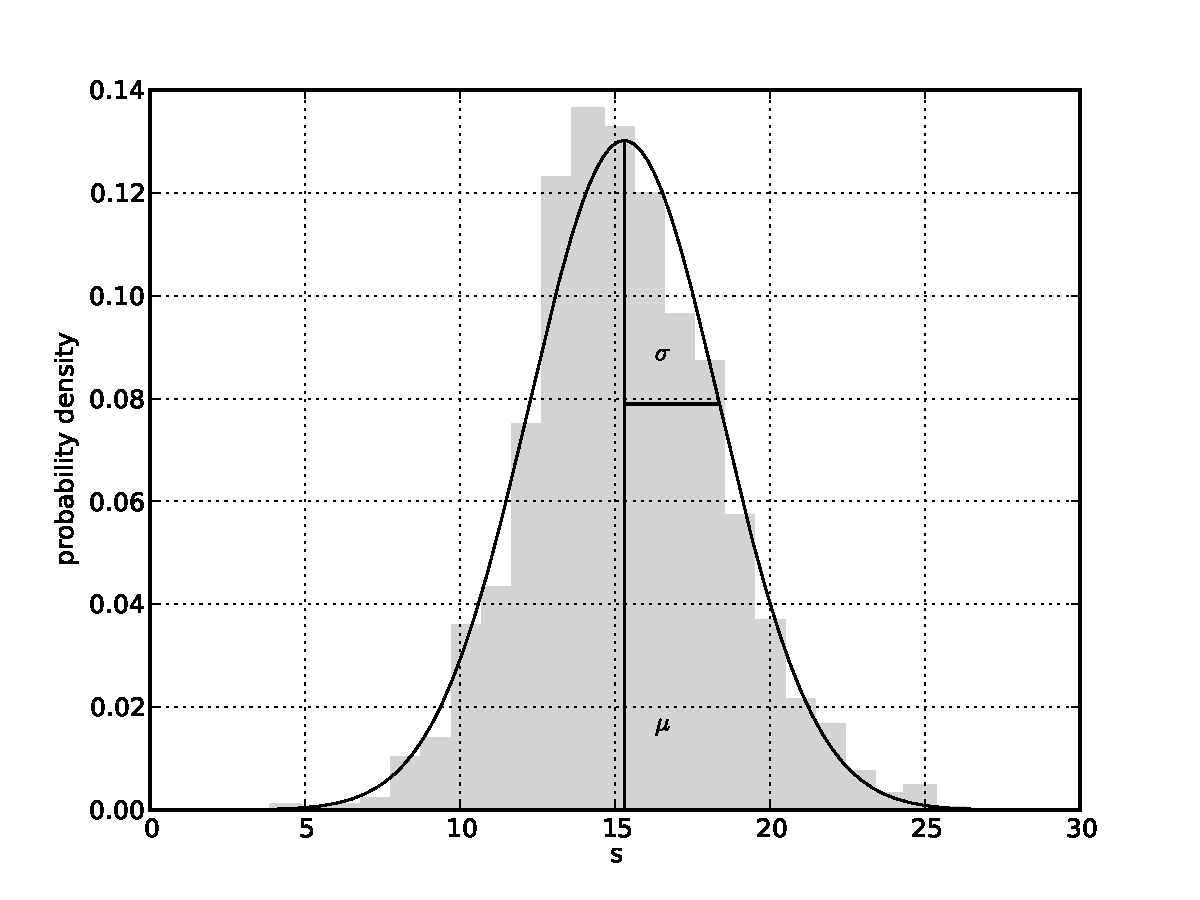
\includegraphics[width=0.9\textwidth]{./present-80-18-14-attack-d-histogram.pdf}
 \caption{4R \emph{Attack-D} on \PRESENT-80-18}
 \label{fig:present-80-18-14-attack-d-histogram}
\end{figure}

\begin{figure}[htbp]
 \centering
 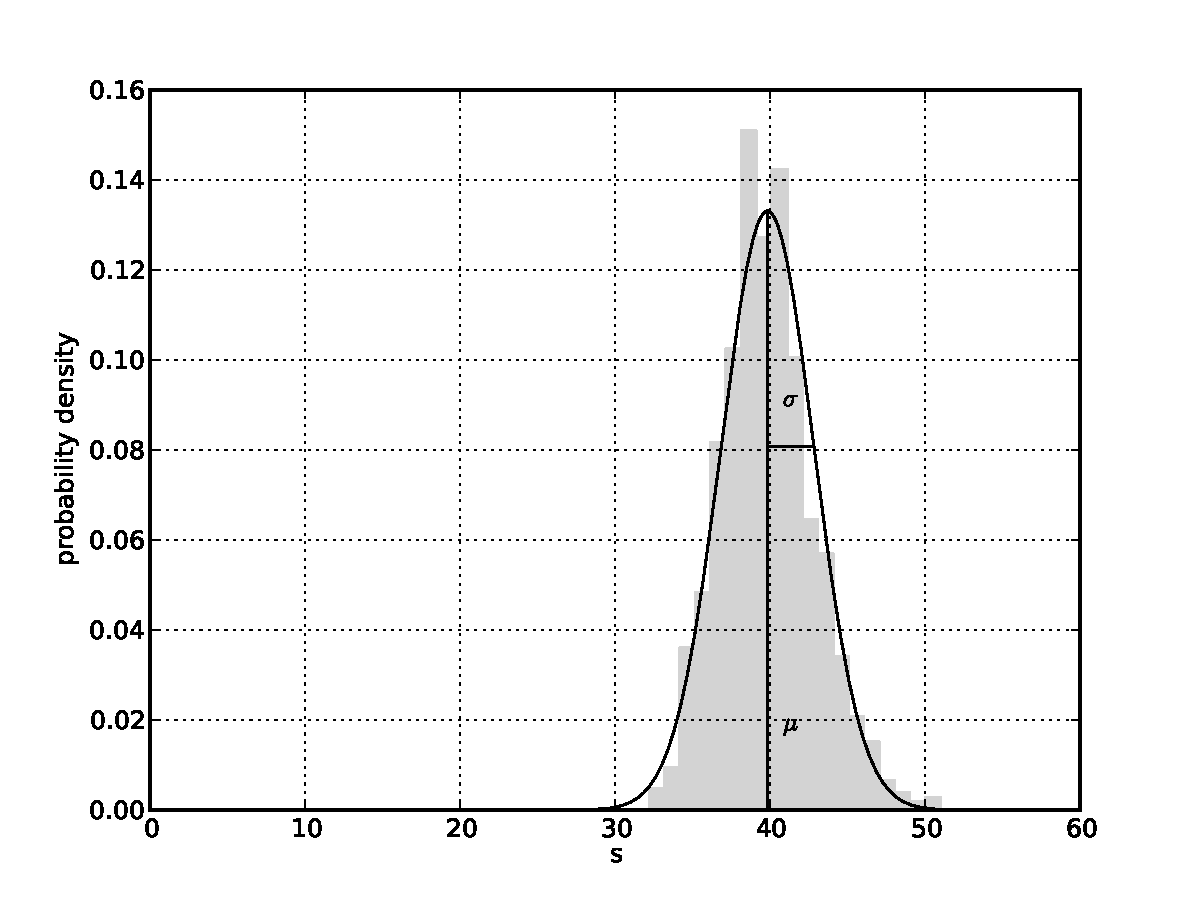
\includegraphics[width=0.9\textwidth]{./present-80-13-10-attack-d-histogram.pdf}
 \caption{3R \emph{Attack-D} on \PRESENT-80-13}
 \label{fig:present-80-13-10-attack-d-histogram}
\end{figure}

\begin{table}[ht]
\begin{center}
\begin{tabular}{|r|r|r|r|r|r|r|r|r|r|r|}
\hline
$s$                         & 22 & 23 & 24 & 25 & 26 & 27 & 28 & 29 & 30 & 31\\  
\hline
$\log_2 \textnormal{Pr}(s)$ & -4.11 & -4.97 & -5.92&  -6.98 & -8.13& -9.39 & -10.76 & -12.23 & -13.80 & -15.48\\
\hline
\end{tabular}
\end{center}
\caption{Probabilities for 4R \emph{Attack-D} against \PRESENT-80-18.}
\label{tab:present-80-18-14-attack-d-prob}
\end{table}


\begin{table}[ht]
\begin{center}
\begin{tabular}{|r|r|r|r|r|r|r|r|r|r|r|}
\hline
$s$                         &   44 &    45 &    46 &    47 &    48 &    49 &    50 &     51 &     52 &     53\\
\hline
$\log_2 \textnormal{Pr}(s)$ & -2.78 & -3.60 & -4.56 & -5.65 & -6.89 & -8.27 & -9.81 & -11.49 & -13.32 & -15.31\\
\hline
\end{tabular}
\end{center}
\caption{Probabilities for 3R \emph{Attack-D} against \PRESENT-80-13.}
\label{tab:present-80-13-10-attack-d-prob}
\end{table}

To check the accuracy of the prediction in Table~\ref{tab:present-80-18-14-attack-d-prob} we tested 1024 random pairs for \PRESENT-80-18 whether they are still solvable with $s=26$. Four of 1024 pairs survived; while the Gauss formulae predicted $2^{10} \cdot 2^{-8.13} \approx 4$ pairs.

By inspection of the Tables~\ref{tab:present-80-14-attack-d} and \ref{tab:present-80-18-attack-d} we can see that right pairs follow a different distribution. Right pairs for \PRESENT-80-18 have $\mu = 28.60$ and $\sigma = 6.55$ (for $t=10$ and $k=4$). Right pairs for \PRESENT-80-14 have  $\mu = 27.71$ and $\sigma=5.09$ (for $t=10$ and $k=3$).

\begin{table}[ht]
\begin{center}
\begin{tabular}{|c|c||r|r|r||r|r|r||r|r|r|}
\hline
Key & Char & \multicolumn{3}{|c||}{2R} & \multicolumn{3}{|c||}{3R} &  \multicolumn{3}{|c|}{4R}\\
\hline
& & $\lfloor s \rfloor$ & $\lfloor s \rceil$ & $\lceil s \rceil$ & $\lfloor s \rfloor$ & $\lfloor s \rceil$ & $\lceil s \rceil$ & $\lfloor s \rfloor$ & $\lfloor s \rceil$ & $\lceil s \rceil$ \\
\hline
\texttt{fc676e7c dad721db 95c7} & 0 & 67 & 69 & 73 & 48 & 50 & 52 & 28 & 30 & 34\\
\hline
\texttt{8e96e4d8 233c16b6 95bc} & 0 & 71 & 73 & 76 & 59 & 60 & 61 & 34 & 37 & 41\\
                                & 1 & 69 & 69 & 71 & 49 & 50 & 52 & 22 & 23 & 26\\
                                & 0 & 72 & 75 & 80 & 65 & 67 & 69 & 44 & 44 & 44\\
\hline
\texttt{04175372 9f035a88 5cc8} & 0 & 69 & 70 & 75 & 48 & 49 & 51 & 24 & 27 & 31\\
\hline
\texttt{57ec0ee8 eefc45f5 d41f} & 0 & 65 & 66 & 69 & 43 & 44 & 48 & 19 & 21 & 26\\
                                & 0 & 70 & 71 & 72 & 46 & 47 & 52 & 19 & 21 & 24\\
                                & 0 & 68 & 69 & 71 & 51 & 52 & 53 & 19 & 20 & 22\\
\hline
\texttt{69550cf3 db7a4820 eb8f} & 0 & 73 & 73 & 75 & 65 & 67 & 70 & 44 & 44 & 44\\
                                & 0 & 69 & 69 & 70 & 55 & 56 & 58 & 23 & 24 & 27\\
                                & 0 & 67 & 68 & 69 & 45 & 46 & 48 & 22 & 24 & 27\\
                                & 0 & 71 & 72 & 74 & 63 & 64 & 66 & 40 & 42 & 44\\
\hline
\texttt{c3ce099f c4c1574c 5785} & 0 & 66 & 67 & 68 & 43 & 44 & 46 & 25 & 27 & 31\\
                                & 0 & 69 & 69 & 71 & 56 & 56 & 57 & 40 & 41 & 44\\
                                & 0 & 66 & 66 & 68 & 44 & 45 & 48 & 25 & 27 & 29\\
                                & 1 & 69 & 70 & 75 & 59 & 61 & 68 & 32 & 35 & 39\\
\hline
\texttt{1c38e1f6 86f0ca45 3c3d} & 1 & 72 & 73 & 76 & 63 & 63 & 64 & 44 & 44 & 44\\
\hline
\end{tabular}
\end{center}
\caption{\emph{Attack-D} results for right pairs for the differential with $r=10$.}
\label{tab:present-80-14-attack-d}
\end{table}

\begin{table}[ht]
\begin{center}
\begin{tabular}{|c|c|r|r|r|}
\hline
$P'$ & $K$ & min. $s$ & avg. $s$ & max. $s$\\
\hline
\texttt{c61bf05c 2a39a5e4} & \texttt{11ec9f16 5edf2206 2eca} & 20 & 21 & 23\\  
\texttt{0538a885 efcc1610} & \texttt{7d227785 08f40902 5443} & 31 & 33 & 39\\  
\texttt{7ff2f485 d5a60d21} & \texttt{e0d9bb12 8807920c 5c08} & 36 & 38 & 40\\  
\texttt{cf9237a3 59636e00} & \texttt{076561d0 4cbd0675 3ee3} & 33 & 35 & 38\\  
\texttt{e9cb5753 e695ef32} & \texttt{4e7cacde 64f8a099 7656} & 16 & 18 & 24\\  
\texttt{adfaf8c6 df732dcf} & \texttt{b53f5586 0b516585 67e8} & 30 & 32 & 34\\  
\texttt{66396df4 366faa43} & \texttt{69b319cb 18b56d0d 2d97} & 33 & 35 & 38\\  
\texttt{25fd6008 9c1bdbfc} & \texttt{05f0e912 e477c457 2bb5} & 28 & 29 & 31\\  
\texttt{544841b2 ce90aa14} & \texttt{1bd3681c eee2ea8d d2e0} & 28 & 31 & 34\\  
\texttt{530c3275 4d0d666f} & \texttt{d403c614 1c074ef5 a629} & 24 & 26 & 28\\  
\texttt{a283ce93 eab76c9d} & \texttt{0d6b63e5 dd806b00 6ef8} & 24 & 26 & 29\\  
\texttt{a1637f3f 6a497c75} & \texttt{b6005536 8fccfbcc ff6f} & 40 & 40 & 40\\  
\texttt{76c6fc0d b9e541ac} & \texttt{2e1f1d8b 46ee7986 3c59} & 18 & 21 & 25\\  
\texttt{7d6f4036 11cfe536} & \texttt{9544bc1c 16dfaddc a8ca} & 27 & 29 & 33\\  
\texttt{0e1fc0e1 43c74365} & \texttt{f952e6db c3c89b47 64a4} & 19 & 21 & 24\\  
\texttt{1eea7d43 37962d04} & \texttt{0eb932ae ae36e58d 1f57} & 22 & 24 & 30\\  
\texttt{26e3ed68 a0f4a62d} & \texttt{218027b0 d3579e80 0321} & 37 & 38 & 40\\  
\texttt{8f5c5ca1 ee230995} & \texttt{c808951c c403fefc 016e} & 27 & 28 & 31\\  
\texttt{a9e16caa 327d0361} & \texttt{f6cd9ff8 7224946e a4db} & 27 & 29 & 32\\  
\texttt{2c795566 739e1b06} & \texttt{bc05d993 8ea6e4f7 f8fb} & 16 & 18 & 21\\  
\texttt{a283ce93 eab76c9d} & \texttt{0d6b63e5 dd806b00 6ef8} & 24 & 26 & 29\\
\texttt{76c6fc0d b9e541ac} & \texttt{2e1f1d8b 46ee7986 3c59} & 18 & 21 & 25\\
\texttt{26e3ed68 a0f4a62d} & \texttt{218027b0 d3579e80 0321} & 37 & 38 & 40\\
\texttt{8f5c5ca1 ee230995} & \texttt{c808951c c403fefc 016e} & 27 & 28 & 31\\
\texttt{a9e16caa 327d0361} & \texttt{f6cd9ff8 7224946e a4db} & 27 & 29 & 32\\
\texttt{2c795566 739e1b06} & \texttt{bc05d993 8ea6e4f7 f8fb} & 16 & 18 & 21\\
\texttt{b9d5ee1a 9ec8298b} & \texttt{c6d9fb3e 9cc686df 69ab} & 20 & 21 & 24\\
\texttt{e09f9557 3a01e584} & \texttt{877b6b0b 203fe2f0 fde3} & 34 & 36 & 39\\
\hline
\end{tabular}
\end{center}
\caption{\emph{Attack-D} against \PRESENT-80-18 and $r=14,k=3,t=10$.}
\label{tab:present-80-18-attack-d}
\end{table}

We can exploit this observation in two ways. First, we may choose to construct a filter. However, this filter will discard both some wrong and some right pairs. For instance, we may choose to discard in a 4R attack any pair for which the average $s$ smaller than $26$. From Table~\ref{tab:present-80-18-14-attack-d-prob} we know that roughly 1 in 256 random pair will survive this filter. Furthermore, from Table~\ref{tab:present-80-18-attack-d} we expect more than half right pairs to survive this filter. Since in most attacks we cannot afford to discard right pairs the filter is mainly of theoretical interest. We note that if we consider $s$ smaller than $18$ we would still cut the number of surviving random pairs by more than half ($\log_2 \textnormal{Pr}(18) = 2^{-1.79}$) while not sacrificing any right pairs with high probability.

A second strategy might be to rank candidate key guesses according to the value $s$. Pairs for which $s$ is large contribute more to a candidate key counter than pairs with small varieties. This might help to identify a peak more quickly.

\subsection{Equations for \emph{Generalised Attack-B} against PRESENT-80}
We consider the first two encryption rounds and the characteristic from \cite{present-dc:africacrypt}. We set up a polynomial ring with two blocks such that the variables $P_i$ and $K_i$ are lexicographically smaller than any other variable. Within the blocks we chose a degree lexicographical monomial ordering. We set up an equation system covering the first two encryption rounds and added the linear equations suggested by the characteristic. Then, we eliminated all linear leading terms which are not in the variables $P_i$ and $K_i$ and computed a Gröbner basis up to degree five. This computation returned 22 polynomials for which we computed the reduced Gröbner basis given below.
\begin{align*}
& {(K_{1} + P'_{1} + 1)} {(K_{0} + K_{3} + K_{29} + P'_{0} + P'_{3})},\\
& {(K_{2} + P'_{2})} {(K_{0} + K_{3} + K_{29} + P'_{0} + P'_{3})},\\
& K_{1} K_{2} + K_{1} P'_{2} + K_{2} P'_{1} + P'_{1} P'_{2} + K_{0} + K_{1} + K_{3} + K_{29} + P'_{0} + P'_{1} + P'_{3},\\
& {(K_{9} + P'_{9} + 1)} {(K_{8} + K_{11} + K_{31} + P'_{8} + P'_{11})},\\
& {(K_{10} + P'_{10})} {(K_{8} + K_{11} + K_{31} + P'_{8} + P'_{11})},\\
& K_{9} K_{10} + K_{9} P'_{10} + K_{10} P'_{9} + P'_{9} P'_{10} + K_{8} + K_{9} + K_{11} + K_{31} + P'_{8} + P'_{9} +
P'_{11},\\
& {(K_{49} + P'_{49} + 1)} {(K_{41} + K_{48} + K_{51} + P'_{48} + P'_{51})},\\
& {(K_{50} + P'_{50})} {(K_{41} + K_{48} + K_{51} + P'_{48} + P'_{51})},\\
& K_{49} K_{50} + K_{49} P'_{50} + K_{50} P'_{49} + P'_{49} P'_{50} + K_{41} + K_{48} + K_{49} + K_{51} + P'_{48} +
P'_{49} + P'_{51},\\
& {(K_{57} + P'_{57} + 1)} {(K_{43} + K_{56} + K_{59} + P'_{56} + P'_{59})},\\
& {(K_{58} + P'_{58})} {(K_{43} + K_{56} + K_{59} + P'_{56} + P'_{59})},\\
& K_{57} K_{58} + K_{57} P'_{58} + K_{58} P'_{57} + P'_{57} P'_{58} + K_{43} + K_{56} + K_{57} + K_{59} + P'_{56} +
P'_{57} + P'_{59},\\
& K_{5} + K_{7} + P'_{5} + P'_{7},\\
& K_{6} + K_{7} + P'_{6} + P'_{7},\\
& K_{53} + K_{55} + P'_{53} + P'_{55},\\
& K_{54} + K_{55} + P'_{54} + P'_{55}.\\
\end{align*}

This system gives 8 bits of information about the key. Note that the first two rounds of the characteristic pass with
probability $2^{-8}$; thus this result is optimal.

\subsection{Equations for \emph{Generalised Attack-B} against KTANTAN32}
We consider the first 24 rounds of KTANTAN32 and compute the full Gröbner basis. This computation recovers 39 polynomials of which we list the 8 smallest non-redundant ones below. Note that the characteristic also imposes restrictions on the plaintext values.
\begin{align*}
& {(P'_{19} + 1)} {(P'_{3} P'_{8} + P'_{10} P'_{12} + K_{3} + K_{53} + P'_{7} + P'_{18} + P'_{23})} ,\\
& P'_{8} P'_{10} P'_{19} + K_{8} P'_{19} + P'_{3} P'_{8} + P'_{6} P'_{19} + P'_{10} P'_{12} + P'_{16} P'_{19} + K_{3} +
K_{53} + P'_{7} + P'_{18} + P'_{19} + P'_{23} ,\\
& P'_{19} P'_{22} + K_{1} + K_{11} + P'_{6} + P'_{11} + P'_{17} + P'_{21} + P'_{26} ,\\
& P'_{23} P'_{26} + K_{65} + P'_{21} + P'_{25} + P'_{30} ,\\
& P'_{1} + 1 , P'_{2} , P'_{5} + 1 , P'_{9} + 1\\
\end{align*}
These eight equations give up to four bits (depending on the value of $P'_{19}$) of information about the key. Due to the simple algebraic structure of KTANTAN32 we can compute more information about the key but we do not explicitly list these polynomials here.

\subsection{\emph{Attack-A} against PRESENT-80-14}
To mount the attack, we generate systems of equations $\overline{F}$ as in Section~\ref{sec:overview} for pairs of encryptions with prescribed difference as described in Section~\ref{sec:present-dc}, by adding linear equations for the differentials predicted by the characteristic given in \cite{present-dc:africacrypt}. For \PRESENT this is equivalent to adding 128 linear equations per round of the form $\Delta X_{i,j} = X_{i,j}' + X_{i,j}''$ and $\Delta Y_{i,j} = Y_{i,j}' + Y_{i,j}''$ where $\Delta X_{i,j}$ and $\Delta Y_{i,j}$ are the values predicted by the characteristic (these are zero for non-active S-Boxes).

We then converted $\overline{F}$ for \PRESENT-80-14 to conjunctive normal form\footnote{For this conversion we represent the S-Box by the principal generator of the ideal spanned by the S-Box polynomials.} using \PolyBoRi's conversion routines (cf.\ Section~\ref{sec:sat}) and use \CryptoMiniSat \cite{SNC09} to solve it.

The timings for \emph{Attack-A} against the right pairs so recovered using a brute-force search are given in Table~\ref{tab:present-attack-a}. The second column indicates whether the pair satisfies the characteristic as well as the differential. In all Tables in this Chapter the symbol $\infty$ denotes that we interrupted the computation after 24 hours.

\begin{table}[ht]
\begin{center}
\begin{tabular}{|l|l|r|}
\hline
Key & Characteristic & Time\\
\hline
\texttt{fc676e7c dad721db 95c7} & False & 73.140s\\
\hline
\texttt{8e96e4d8 233c16b6 95bc} & False & 9865.350s\\
                                & True  & 6.220s\\
                                & False & $\infty$\\
\hline
\texttt{04175372 9f035a88 5cc8} & False & 44.720s\\
\hline
\texttt{57ec0ee8 eefc45f5 d41f} & False & 16.480s\\
                                & False & 15.250s\\
                                & False & 14.850s\\
\hline
\texttt{69550cf3 db7a4820 eb8f} & False & $\infty$\\
                                & False & 16.550s\\
                                & False & 17.720s\\
                                & False & $\infty$\\
\hline
\texttt{c3ce099f c4c1574c 5785} & False & 125.570s\\
                                & False & $\infty$\\
                                & False & 50.360s\\
                                & True  & 780.190s\\
\hline
\texttt{1c38e1f6 86f0ca45 3c3d} & False & $\infty$\\
\hline
\end{tabular}
\end{center}
\caption{Timings for \emph{Attack-A} against \PRESENT-80-14 and $r=10$.}
\label{tab:present-attack-a}
\end{table}

While in Table~\ref{tab:present-attack-a} not all instances were solved within the allowed time of 24 hours, we can see that there are indeed instances where the full key is recovered.

We also ran $2^{14}$ trials on random instances of \PRESENT-80-14 with $r=10$ to gain an insight into the average running time over random candidate pairs. The average running time was $1.294$ seconds on a 2.66~Ghz Xeon server. Thus we expect the overall attack to take $2^{44}$ applications of \emph{Symbolic Attack-C} and $2^{44 -3.082} \cdot 1.294 \cdot 2.66 \cdot 10^9 \approx 2^{72.60}$ CPU cycles. We assume that a single encryption costs at least two CPU cycles per round -- one for the S-Box lookup and one for the key addition -- such that a brute force search would require approximately $14 \cdot 2 \cdot 2^{80} \approx 2^{84.80}$ CPU cycles and two plaintext--ciphertext pairs due to the small block-size.

We can extend this 4R attack to a 5R attack. We consider the input difference for round 11 and iterate over all possible output differences. As discussed in Section~\ref{sec:present-dc}, we have six possible output differences and two active S-Boxes in round 11, which result in 36 possible output differences in total. We expect a 5R attack on \PRESENT-80-15 to cost $36 \cdot 2^{72.60} \approx 2^{77.77}$ CPU cycles with a data complexity of $2^{44}$ chosen plaintext-ciphertext pairs under the assumption that we can mount an \emph{Symbolic Attack-C} which will pass for at most one out of $2^{3.082}$ pairs for each of the 36 output differences of round 11. By the same argument we can consider all $2^{13.94}$ possible output differences for round 12. Thus a 6R attack on \PRESENT-80-16 would cost $2^{13.94} \cdot 2^{72.60} \approx 2^{86.54}$ CPU cycles which is worse than exhaustive key search if our conservative estimate of 2 CPU cycles per round is assumed\footnote{Our bit-slice implementation of \PRESENT achieves 16.5 cycles per round on a 2.33Ghz \CTD.}.

\subsection{\emph{Attack-A} against KTANTAN32}
We consider KTANTAN32-113 and the aforementioned 71 round characteristic which holds with probability $2^{-31}$ disregarding any dependencies. Using a SAT solver we computed right pairs. Then we construct an equation system for this right pair and attempt to solve it. In order to ensure a unique solution, we add an equation system for a third encryption of a random plaintext under the same key. We tried 10 such experiments and always recovered the right key in under one minute using the SAT solver \CryptoMiniSat. We note that the attack does not scale further (cf.\  Table~\ref{tab:ktantan32-b-minisat2}).

\subsection{\emph{Attack-B} and \emph{Attack-C} against PRESENT}
To perform the algebraic part of the attack, we use either Gröbner basis algorithms or a SAT solver: 
\begin{itemize}
 \item the \textsc{PolyBoRi}~\cite{polybori} routine \texttt{groebner\_basis} with the option \texttt{faugere=True} and the monomial ordering \texttt{dp\_asc},
 \item the \textsc{Singular}~3-0-4-4~\cite{singular} routine \texttt{groebner} with the monomial ordering \emph{degrevlex},
 \item \MiniSat \cite{minisat}.
\end{itemize}
We recorded the maximal time $t$ these routines take to detect a contradiction in our experiments for a given characteristic of length $r$.

We note that SAT solvers should be the most adequate tools for this task. Recall that \PRESENT has a block size of 64-bit and a key size of either 80 or 128 bits. Thus for each encryption mapping $P$ to $C$ there are about $2^{16}$ or $2^{64}$ different keys on average which satisfy the map. The same applies to the related ``cipher'' constructed in \emph{Attack-C}. However, writing down $2^{64}$ solutions algebraically is likely too expensive both with respect to time as well as memory. Thus, we cannot expect the Gröbner basis calculation to finish within reasonable time and the computation has to be aborted after some time-out $t$. This however leaves the question whether a contradiction would have been found afterwards if the computation would not have been interrupted. On the other hand, finding one single solution certifies that the related ``cipher'' constructed in \emph{Attack-C} is satisfiable, i.e. that the pair of ciphertexts is compatible with the differential under some key. This task is exactly what SAT solvers are optimised for.

We performed experiments for \emph{Attack-B} and \emph{Attack-C}. Runtimes for \emph{Attack-B} and \emph{Attack-C} are given in
Table~\ref{tab:present-att-b} and~\ref{tab:present-att-c} respectively. We note that Attack-C requires about 1GB of RAM to be carried out.
The times were obtained on a 1.8Ghz Opteron with 64GB RAM.

\begin{table}
\begin{center}
\begin{tabular}{|c|c|c|c|c|c|c|c|}
\hline
$N$ & $K_s$ & $r$ & $p$ & \#trials & \textsc{Singular}& \#trials & \textsc{PolyBoRi}\\
\hline
 4 &  80 &  4 & $2^{-16}$ & 20 & $11.92-12.16$   & 50 & $0.72 - 0.81$ \\
 4 &  80 &  3 & $2^{-12}$ & 10 & $106.55-118.15$ & 50 & $6.18 - 7.10$ \\
 4 &  80 &  2 &  $2^{-8}$ & 10 & $119.24-128.49$ & 50 & $5.94 - 13.30$ \\
 4 &  80 &  1 &  $2^{-4}$ & 10 & $137.84-144.37$ & 50 & $11.83 - 15.485$
\\
\hline
 6 &  80 &  6 & $2^{-26}$ & 0 &  N/A               & 50 & $0.86 - 0.95$ \\
 6 &  80 &  5 & $2^{-22}$ & 0 &  N/A               & 25 & $11.93 - 13.74$ \\
\hline
 8 &  80 &  5 & $2^{-22}$ & 0 &  N/A               & 50 & $18.45 - 63.21$\\
\hline
10 &  80 & 10 & $2^{-44}$ & 0 &  N/A               & 20 & $3.24-3.92$ \\
10 &  80 &  9 & $2^{-40}$ & 0 &  N/A               & 20 & $21.43-26.41$ \\
10 &  80 &  8 & $2^{-34}$ & 0 &  N/A               & 20 & $21.73-38.96$ \\
10 &  80 &  7 & $2^{-30}$ & 0 &  N/A               & 10 & $39.27 - 241.17$\\
10 &  80 &  6 & $2^{-26}$ & 0 &  N/A               & 20 & $56.30 - >4$ hours\\
\hline
16 &  80 & 14 & $2^{-62}$ & 0 & N/A                & 20 & $43.42-64.11$ \\
16 & 128 & 14 & $2^{-62}$ & 0 & N/A                & 20 & $45.59-65.03$ \\
16 &  80 & 13 & $2^{-58}$ & 0 & N/A                & 20 & $80.35-262.73$\\
16 & 128 & 13 & $2^{-58}$ & 0 & N/A                & 20 & $81.06-320.53$ \\
16 &  80 & 12 & $2^{-52}$ & 0 & N/A                & 5 & $>4$ hours\\
16 & 128 & 12 & $2^{-52}$ & 0 & N/A                & 5 & $>4$ hours \\
\hline
17 &  80 & 14 & $2^{-62}$ & 10 & $12,317.49-13,201.99$ & 2048 & $11.996 - 46.656$\\
17 & 128 & 14 & $2^{-62}$ & 10 & $12,031.97-13,631.52$ & 512 & $13.26 - 48.142$\\
17 &  80 & 13 & $2^{-58}$ & 0 & N/A                & 5 & $>4$ hours\\
17 & 128 & 13 & $2^{-58}$ & 0 & N/A                & 5 & $>4$ hours\\
\hline
\end{tabular}
\end{center}
\caption{Experimental results for \emph{Attack-B} against \PRESENT.}
\label{tab:present-att-b}
\end{table}

\begin{table}
\begin{center}
\begin{tabular}{|c|c||c|c|c|c|c|c|}
\hline
$N$ & $K_s$ & $r$ & $p$ & \#trials & \textsc{PolyBoRi} & \#trials & \MiniSat\\
\hline
 4 &  80 &  4 & $2^{-16}$ & 50 & $0.05 -  0.06$ &  0 & N/A\\
 4 &  80 &  3 & $2^{-12}$ & 50 & $0.88 -  1.00$ & 50 & 0.14 - 0.18\\
 4 &  80 &  2 &  $2^{-8}$ & 50 & $2.16 -  5.07$ & 50 & 0.32 - 0.82\\
 4 &  80 &  1 &  $2^{-4}$ & 50 & $8.10 - 18.30$ & 50 & 1.21 - 286.40\\
\hline
16 &  80 & 14 & $2^{-62}$ & 50 & 2.38 -  5.99 & 1024 & $0.012 - 0.018$\\
16 & 128 & 14 & $2^{-62}$ & 50 & 2.38 -  5.15 & 0 & N/A\\
16 &  80 & 13 & $2^{-58}$ & 50 & 8.69 - 19.36 & 0 & N/A\\
16 & 128 & 13 & $2^{-58}$ & 50 & 9.58 - 18.64 & 0 & N/A\\
16 &  80 & 12 & $2^{-52}$ &  5 & $>$4 hours   & 0 & N/A\\
\hline
17 &  80 & 14 & $2^{-62}$ & 1024 & $3.193 - 3.900$ & 1024 & $0.012 - 0.032$\\
17 & 128 & 14 & $2^{-62}$ & 2048 & $3.444 - 5.440$ & 1024 & $0.008 - 0.032$\\
17 &  80 & 13 & $2^{-58}$ &  5 & $>4$ hours   &  5 & $>4$ hours\\
\hline
\end{tabular}
\end{center}
\caption{Experimental results for \emph{Attack-C} against \PRESENT.}
\label{tab:present-att-c}
\end{table}

\subsubsection{PRESENT-80-16}
To compare with the results of~\cite{present-dc:africacrypt}, we can apply a series of attacks against reduced round versions of \PRESENT-80. We expect to learn 8 bits of information about the key for \PRESENT-80-16 in about $2^{62-51.669} \cdot t$ seconds to run \emph{Attack-B} using about $2^{62}$ chosen plaintext--ciphertext pairs, where $t$ represents the expected average runtime. This time gives a complexity of about $2^{62}$ ciphertext difference checks and about $2^{10.331} \cdot t \cdot 1.8 \cdot 10^9 \approx 2^{41.07} \cdot t$ CPU cycles to find a right pair on the given 1.8~Ghz Opteron CPU. We assume that a single encryption costs at least two CPU cycles per round -- one for the S-Box lookup and one for the key addition -- such that a brute force search would require approximately $16 \cdot 2 \cdot 2^{80} = 2^{85}$ CPU cycles and two plaintext-ciphertext pairs due to the small block-size. Thus $t$ must be smaller than $2^{43.93}$ CPU cycles on average to beat exhaustive key search.

In~\cite{present-differentials}, 24 different 14-round differentials were given, involving the $0^{\textnormal{th}}$, $1^{\textnormal{st}}$, $2^{\textnormal{nd}}$, $12^{\textnormal{th}}$, $13^{\textnormal{th}}$ and $14^{\textnormal{th}}$ S-Boxes in the first round, each having either \texttt{0x7} or \texttt{0xF} as plaintext difference restricted to one active S-Box. From these we expect to recover 18 bits of key information from the first round by repeating the attack for those S-Box configurations. We cannot recover 24 bits from the first round because we learn some redundant information; however, we can use this redundancy to verify the information recovered so far. On the other hand, we expect to learn more information from the second round (cf.~\emph{Generalised Attack-B}). We can then guess the remaining $80-18 = 62$ bits, and the complete attack has a complexity of about $6  \cdot 2^{62}$ filter function applications, about $6 \cdot
2^{41.07} t$ CPU cycles for the consistency checks and $2^{62}$ \PRESENT applications to guess the remaining key bits\footnote{Note that the attack can be improved by managing the plaintext--ciphertext pairs more intelligently and by using the fact that we can abort a \PRESENT trial encryption if it does not match the known differential.}. Alternatively, we may add the 18 learned linear key bit equations to our equation system and attempt to solve this system. The attack in~\cite{present-dc:africacrypt} on the other hand requires $2^{64}$ memory accesses. While this is a different metric --- memory access --- from the one we have to use in this case --- CPU cycles --- we can see that our approach has a slightly better data complexity because overall six right
pairs are sufficient. However, we cannot be certain about the exact value of $t$ and thus the exact time complexity of our attacks. When applying the attack against \PRESENT-128-16, we obtain a similar complexity.

\subsubsection{PRESENT-128-17}
We apply our techniques to \PRESENT-128-17. We expect to learn 4 bits of information for \PRESENT-128-17 in about $2^{62 - 18.296} \cdot t$ seconds using about $2^{62}$ chosen plaintext-ciphertext pairs and \emph{Symbolic Attack-C} applications. We filter pairs in three stages: \emph{Symbolic Attack-C}, \emph{Attack-C} and \emph{Attack-B}. We expect exhaustive key search to cost $17 \cdot 2.0 \cdot 2^{128} \approx 2^{133}$ CPU cycles. Thus, in order to beat exhaustive key search, $t$ must be smaller than $2^{89}$ CPU cycles on average such that we have $2^{133} > 2^{43.73} \cdot t$.

\subsubsection{PRESENT-128-18}
We may be able to attack \PRESENT-128-18 using our attacks if we assume that we can identify a right pair with very high probability in time $t$ for a 3R attack. For this, we consider the input difference for round 15 and iterate over all possible output differences. As discussed in Section~\ref{sec:present-dc}, we have six possible output differences and two active S-Boxes in round 15, which result in 36 possible output differences in total. We expect to learn 4 bits of information about the key for \PRESENT-128-18 in about $36 \cdot 2^{62-q} \cdot t$ seconds using about $2^{62}$ chosen plaintext-ciphertext pairs where $q$ is such that 1 in $2^q$ pairs is accepted by \emph{Attack-C}.

\subsubsection{PRESENT-128-19}
Similarly, we  may be able to use our attacks to mount an attack against \PRESENT-128-19 by iterating our attack $2^{64-50.669} = 2^{13.331}$ times (instead of 36) for all possible output differences of round 16.


\subsubsection{Combining \emph{Attack-B} and \emph{Attack-C}}
In order to gain more precise filters, we may add rounds prior to the round $r$ to our equation system constructed in \emph{Attack-C}. Instead of either stopping at round $r$ (counting from the rear) or going all the way (i.e. using the differential characteristic), we may choose to add for example four more rounds prior to the round $r$. As Table~\ref{tab:present-bc} shows, this indeed improves the precision of the filter at the cost of being potentially more expensive.

\begin{table}[htbp]
\begin{center}
\begin{tabular}{|c|c|c|c|c|c|c|c|c|}
\hline
$K_s$ & $N$ & $r$  & pre-$r$ & \#trials & \#passes & $t$ in seconds &  avg. $t$ & quality\\
\hline
128 & 18 &  14 & 0 & 8192 & 948 & $0.152 - 1.560$ & $0.176$ & $\approx 2^{-3.11}$\\
128 & 18 &  14 & 4 & 8192 & 924 & $0.168 - 0.868$ & $0.226$ & $\approx 2^{-3.15}$\\
\hline
 80 & 18 & 14 & 0 & 8192 & 977 & $0.152 - 9.289$ & $0.262$ & $\approx 2^{-3.07}$\\
 80 & 18 & 14 & 4 & 8192 & 191 & $0.164 -  784.737$ & $9.576$ & $\approx 2^{-5.42}$\\
\hline
\end{tabular}
\end{center}
\caption{Compromise between \emph{Attack-B} and \emph{Attack-C}.}
\label{tab:present-bc}
\end{table}


\subsection{\emph{Attack-B} against KTANTAN32}

We report minimum, average, median and maximum running times for \emph{Attack-B} using \PolyBoRi 0.6.3 in Table~\ref{tab:ktantan32-b-polybori}. In Table~\ref{tab:ktantan32-b-polybori} $N_r$ denotes the number of rounds of the cipher, $r$ the number of rounds covered by the characteristic, $p$ the probability that the characteristic holds.

\begin{table}[ht]
\begin{center}
\begin{tabular}{|c|c|c|c|c|c|c|c|}
\hline
$N_r$ & $r$ & $\log_2 p$ & $t_{min}$ & $t_{avg}$ & $t_{med}$ & $t_{max}$ & $\log_2 \#$trials\\
\hline
 91 & 71 & -31 & 0.050 & 0.059 & 0.060 & 0.260 & 14\\
 96 & 71 & -31 & 0.050 & 0.065 & 0.060 & 0.290 & 14\\
100 & 71 & -31 & 0.050 & $\infty$ & $\infty$ & $\infty$ & 12\\ 
110 & 71 & -31 & 0.050 & $\infty$ & $\infty$ & $\infty$ & 3\\ 
110 & 71 & -31 & $\infty$ & $\infty$ & $\infty$ & $\infty$ & 0\\ 
\hline
\end{tabular}
\end{center}
\caption{\emph{Attack-B} against KTANTAN32 using \PolyBoRi.}
\label{tab:ktantan32-b-polybori}
\end{table}

In Table~\ref{tab:ktantan32-b-minisat2} we report minimum, average, median and maximum running times for \emph{Attack-B} against KTANTAN32 using the SAT solver \MiniSat. The conversion from algebraic normal form to conjunctive normal form is done using the conversion available in \PolyBoRi (cf. Section~\ref{sec:sat}). The column ``passess'' denotes how often the SAT solver returned an assignment which satisfies the system. The high number of passes in the first row can be explained by the fact that two parallel executions of KTANTAN32 encrypt 64 bits under an 80-bit key.

\begin{table}[ht]
\begin{center}
\begin{tabular}{|c|c|c|r|r|r|r|r|r|}
\hline
 $N_r$ & $r$ & $\log_2 p$ & passes & $t_{min}$ & $t_{avg}$ & $t_{med}$ & $t_{max}$ & $\#$trials\\
\hline
 84 & 42 & -12 & 10 & 0.540 & 38.011 & 34.030 & 243.355 & 1024\\
113 & 71 & -31 &  0 & 0.000 &  2.477 & 0.000 & 1028.220 & 24576\\
116 & 71 & -31 &  0 & 0.000 & 19.370 & 0.000 &  1928.350 & 4096\\ %control=False
120 & 71 & -31 & -- & 0.000 & $\infty$ & $\infty$ & $\infty$ & 55\\
\hline
\end{tabular}
\end{center}
\caption{\emph{Attack-B} against KTANTAN32 using \MiniSat.}
\label{tab:ktantan32-b-minisat2}
\end{table}



\section{Discussion of our Techniques}
\label{sec:discussion}
While our techniques, in particular \emph{Attack-B} and \emph{Attack-C}, have many similarities with conventional differential cryptanalysis, such as the requirement of a high probability differential $\Delta$ valid for $r$ rounds and the use of filter functions to reduce the workload, there are however some noteworthy differences. First, these attacks require fewer plaintext-ciphertext pairs for a given differential characteristic to learn information about the key than conventional differential cryptanalysis, because the attacker does not need to wait for a peak in the partial key counter. Instead one right pair is sufficient. Second, one flavour of the attack recovers more key bits if many S-Boxes are active in the first round. This follows from its reliance on those S-Boxes to recover key information. Also note that while a high probability differential characteristic is required, the attack recovers more bits per S-Box if the differences for the active S-Box in the first round are of low probability. 

Key-recovery differential cryptanalysis is usually considered infeasible if the differential $\Delta$ is valid for $r$ rounds, and $r$ is much less than the full number of rounds $N$, since backward key guessing for $N-r$ rounds may become impractical. In that case the \emph{Attack-C} proposed here could \emph{possibly} still allow the successful cryptanalysis of the cipher. However, this depends on the algebraic structure of the cipher, as it may be the case that the time required for the consistency check and recovery of a candidate key is such that the overall complexity remains below the one required for exhaustive key search.

We note that the attacks B and C share many properties with the differential cryptanalysis of the full 16-round DES \cite{fulldes-dc}. Both are capable of detecting a right pair without maintaining a candidate key counter array. Also, both use active S-Boxes of the outer rounds to recover bits of information about the key once such a right pair is found. In fact, one could argue that the attacks B and C are a generalised algebraic representation of the technique presented in \cite{fulldes-dc}. From this technique attacks B and C inherit some interesting properties: first, the attacks can be carried out fully in parallel because no data structures such as a candidate key array need to be shared between the nodes. Also, we allow the encryption keys to change during the data collection phase because exactly one right pair is sufficient to learn some key information. However, if we try to learn further key bits by repeating the attack with other characteristics we require the encryption key not to change. We note however that while the attack in \cite{fulldes-dc} seems to be very specific to the target cipher DES, these attacks can in principle be applied to any block cipher. 

In the particular case of \PRESENT-80-$N$, our attacks B and C seems to offer only marginal advantage when compared with the differential attack presented in~\cite{present-dc:africacrypt}: they should require slightly less data to distinguish a right pair and similar overall complexity. On the other hand, for \PRESENT-128-$N$ this attack seems to perform better than the one in~\cite{present-dc:africacrypt}. As in this case the limiting factor is the data and not the time complexity of the attack, i.e. we run out of plaintext-ciphertext pairs before running out of computation time, the attack has more flexibility. 

The use of Gr\"obner bases techniques to find contradictions in propositional systems is a well known idea \cite{Clegg1996}. In the context of cryptanalysis, it is also a natural idea to try to detect contradictions to attack a cipher. However, in probabilistic approaches used in algebraic attacks, usually key bits are guessed. This is an intuitive idea because polynomial systems tend to be easier to solve the more over-defined they are and because the whole system essentially depends on the key. Thus guessing key bits is a natural choice. However this simplification seems to bring few benefits to the attacker, and more sophisticated probabilistic approaches seem so far to have been ignored. The method proposed in this chapter can thus highlight the advantages of combining conventional (statistical) cryptanalysis and algebraic cryptanalysis. By considering differential cryptanalysis we showed how to construct an equation system for a structurally weaker and shorter related ``cipher'' which can then be studied independently. To attack this ``cipher'' algebraic attacks seem to be the natural choice since very few "plaintext--ciphertext" pairs are available but the ``cipher'' has few rounds (i.e. $2R-1$). However, other techniques might also be considered.

Variants of \emph{Attack-B} and \emph{Attack-C}, namely \emph{Generalised Attack-B} and \emph{Symbolic Attack-C}, can be used to improve filter functions and the amount of data recovered from a right pair in differential cryptanalysis. Since Gröbner basis computations are only performed in an offline or precomputation phase or only once per right pair candidate, we expect that they are applicable to a wider range of situations than \emph{Attack-B} and \emph{Attack-C}. Furthermore, \emph{Attack-D} highlights algebraic structures in equation systems arising from differential cryptanalysis which are not obvious and might be beneficial in the cryptanalysis of a given cipher.

We note that our attacks may also offer a high degree of flexibility for improvements. For example, the development of more efficient algorithms for
solving systems of equations (or good algebraic representation of ciphers that may result in more efficient solving) would obviously improve the attacks
proposed. For instance, by switching from \textsc{Singular} to \textsc{PolyBoRi} for \emph{Attack-B}, we were able to make the consistency check up to $60$ times faster\footnote{We did not see any further speed improvement by using e.g. \textsc{Magma}~2.14~\cite{magma}}. As an illustration of the aforementioned flexibility, if for instance an attacker could make use of an optimised method to find contradictions in $t \ll 2^{128-62} = 2^{66}$ CPU cycles in an \emph{Attack-B} style system for \PRESENT-128-20, this would allow the successful cryptanalysis of a version of \PRESENT\ with 6 more rounds than the best known differential, which is considered ``a situation without precedent'' by the cipher designers~\cite{present}. Unfortunately with the available computer resources, we are not able to verify whether this is currently feasible.


\chapter{Algebraic Techniques in Higher Order Differential Cryptanalysis}
\label{chapter:algebraic_integral_cryptanalysis}
In this chapter we consider algebraic techniques in higher order differential attacks. Some of the results in this chapter are published in the paper ``Algebraic Precomputations in Differential and Integral Cryptanalysis'' by Carlos Cid, Thomas Dullien, Jean-Charles Faugère, Ludovic Perret and the author \cite{acdfp:inscrypt2010}. Some of the results against round reduced variants of the block cipher KTANTAN-32 were presented in the rump session of the Early Symmetric Cryptography Seminar 2010 in Remich, Luxemburg.

\section{Introduction}
\label{sec:algebraic-integral-attacks}
Higher order differentials (HOD) were introduced by Lars Knudsen in \cite{Knudsen1995}. We can define the derivative of a function as follows:

\begin{definition}[Lai \cite{Lai1994}] Let $(S, +)$ and $(T, +)$ be Abelian groups. For a function $f: S \rightarrow T$, the derivative of $f$ at the point $a \in S$ is defined as $$\Delta_a f(x) = f(x+a) - f(x).$$
The $i^{\textnormal{th}}$ derivative of $f$ at the points $a_0,\dots,a_{i-1}$ is defined as $$\Delta^{(i)}_{a_0,\dots,a_{i-1}} f(x) = \Delta_{a_{i-1}} (\Delta_{a_0,\dots,a_{i-2}}^{(i-1)} f(x)).$$
\end{definition}

For the following we assume that we work over $\GFZ$, that is $f: \F_2^k \rightarrow \F_2$. Let $L[a_0,\dots,a_{N-1}]$ be the set of all linear combinations of $a_0,\dots,a_{N-1}$. We have that $$ \Delta^{(N)}_{a_0,\dots,a_{N-1}} f(x) = \sum_{\delta \in L[a_0,\dots,a_{N-1}]} f(x + \delta).$$

If $a_0,\dots,a_{N-1}$ are linearly dependent, we have that $\Delta^{(N)}_{a_0,\dots,a_{N-1}} f(x) = 0$.

The differentials used in differential cryptanalysis correspond to first order derivatives. It thus makes sense to consider higher order differentials. That is, the attacker considers higher order derivatives which hold with high probability for an input set related by $L[a_0,\dots,a_{N-1}]$. This idea was later specialised by Knudsen to the \emph{square attack} where one input byte of a byte-oriented SP-network takes all possible values while all other bytes remain fixed. Attacks where one byte takes all possible values like in the square attack are also referred to as \emph{integral attacks} and these attacks have been used to attack a wide variety of byte-oriented ciphers.

In \cite{bit-pattern-ia} Muhammad Reza Z'Aba, Håvard Raddum, Matt Henricksen and Ed Dawson extend the notion of integral attacks to bit-oriented ciphers, that is ciphers which do not perform operations on a byte basis but on a bit level. In \cite{bit-pattern-ia} the authors consider the block ciphers \PRESENT, NOEKEON and Serpent.

The first work combining algebraic and higher-order differential attacks is \cite{algebraic-higher-order-dc} by Jean-Charles Faugère and Ludovic Perret. The authors use 
higher-order differentials to explain the improved performance of their Gröbner basis based attacks against the Curry and Flurry families of block ciphers \cite{flurry-curry}. 

The following discussion of algebraic and higher-order differential attacks is taken from \cite{algebraic-higher-order-dc}.

First, consider the simplest case where the number of points is $N=2$ and we have $a_0 = \delta_0$. Let $T_{K_i}(\textbf{X}_i)$ be the round function of some block cipher with the round key $K_i$; variables typesetted  bold represent vectors of variables. Select a random message $P'$ and a difference $\delta_0$ and construct an equation system $\overline{F}$ for $P',C'$ and $P'',C''$ where $P'' = P' + \delta_0$. We have there are polynomials in the ideal $I$ spanned by $\overline{F}$ which correspond to
\begin{eqnarray*}
\textbf{X}_1' - T_{K_1}(P') = \textbf{0} \textnormal{ and }
\textbf{X}_1'' - T_{K_1}(P' + \delta_0) = \textbf{0}.
\end{eqnarray*}
This in turn implies that $\textbf{X}_1' - \textbf{X}_1''- \Delta_{\delta_0} T_{K_1}(P')$, where $\Delta_{\delta_0} T_{K_1}(P')$ is some constant, is in the ideal $I$. This fact is exploited in  Chapter~\ref{chapter:algebraic_differential_cryptanalysis} where we guess $\Delta_{\delta_0} T_{K_1}(P')$ explicitly.

We can iterate the process. Let $a_0,\dots a_{N-1}$ be a set of $N ≥ 1$ linearly dependent vectors, and $P'$ be an arbitrary plaintext. We consider the ideal
$$I^N = \left\langle \bigcup_{a \in L[a_0,\dots,a_{N-1}]} F(P' \oplus a, T_{K_i}(P' \oplus a))\right\rangle$$
where $F(P,C)$ is the polynomial system implied by the encryption of $P$ to $C$.

We will denote by $\textbf{X}_i^{(j)}$ the intermediates variables used at the $i^{\textnormal{th}}$ round and corresponding to the $j^\textnormal{th}$ message. For the first round, we have that for all $k$, $0 ≤ k < \#L[a_0\dots,a_{N-1}]$:
$$\textbf{X}_1^{(k)} − \textbf{X}_1^{(0)} - \Delta_aT_{K_1}(P') \in I^N, \textnormal{ with } a \in L[a_0 ,\dots, a_{N-1}].$$
As previously, we have shown that there exist polynomials of low degree in the ideal corresponding to derivatives. But, we will also create equations corresponding to the higher order derivatives. For instance, let $a_0, a_1 \in L[a_0,\dots,a_{N-1}]$. We have:
\begin{eqnarray*}
\textbf{X}_1^{(0)} − T_{K_1} (P' ) \in I^N &, & \textbf{X}_1^{(2)} − T_{K_1} (P' \oplus a_0 ) \in I^N,\\
\textbf{X}_1^{(1)} − T_{K_1} (P' \oplus a_1 ) \in I^N &, &  \textbf{X}_1^{(3)} − T_{K_1} (P' \oplus a_0 \oplus a_1) \in I^N.
\end{eqnarray*}

Therefore $\textbf{X}_1^{(3)} − \sum_{k=0}^{2} \textbf{X}_1^{(k)} - \Delta_{a_0,a_1} T_{K_1}(P') \in I^N$. Moreover, if $a_0$ and $a_1$ are linearly dependent, then $\Delta_{a_0,a_1} T_{K_1}(P')$ is equal to zero. Thus, the ideal  $I^N$ will include linear relations between the intermediates variables $\textbf{X}_1^{(j)}$. Then, such new linear equations will induce derivatives and high order derivatives in the subsequent rounds of the cipher. In our case, where $a_0$ and $a_1$ are linearly dependent we know that $\textbf{X}_1^{(3)} = \sum_{k=0}^{2} \textbf{X}_1^{(k)}$.
If we consider the second round, we have:
$$\textbf{X}_2^{(0)} - T_{K_2}(\textbf{X}_1^{(0)}) \in I^N, \textnormal{ and } \textbf{X}_2^{(3)} - T_{K_2}(\textbf{X}_1^{(0)} + \textbf{X}_1^{(1)} + \textbf{X}_1^{(2)}) \in I^N.$$
This implies that the equations $\textbf{X}_2^{(3)} − \textbf{X}_2^{(0)} = \Delta_{\textbf{X}_1^{(1)} + \textbf{X}_1^{(2)}} T_{K_2} (\textbf{X}_1^{(0)})$ is in the ideal $I^N$. This approach can be iterated for generating differentials of higher orders and thus new polynomials between the intermediates variables of later rounds.

In \cite{algebraic-higher-order-dc} these polynomials are implicit, that is they are not explicitly added to the initial polynomial system. Of course, the mere existence of such polynomials in the ideal does not imply that a Gröbner basis algorithm will be able to find such equations and exploit them. However, we expect these polynomials to be relatively easy to find because they involve only variables from the first few rounds. Indeed, experimental evidence suggests that this technique  reduces the maximum degree reached during a Gröbner basis computation (cf.~\cite{algebraic-higher-order-dc} and Section~\ref{sec:ahod-experiments}).

\section{Experimental Results}
\label{sec:ahod-experiments}

In this section we apply algebraic higher-order differential (AHOD) attacks to reduced round variants of the block ciphers \PRESENT and KTANTAN32.

\subsection{PRESENT}

In \cite{bit-pattern-ia} \emph{bit-pattern based integral attacks} against up to 7 rounds of \PRESENT are proposed. These attacks are based on a 3.5 round distinguisher. The attacker prepares 16 chosen plaintexts which agree in all bit values except the bits at the positions 51, 55, 59, 63. These four bits take all possible values $(0,0,0,0),(0,0,0,1),\dots,(1,1,1,1)$. In \cite{bit-pattern-ia} the authors show that the input bits to the 4th round are then balanced. That is, the sum of all bits at the same bit position across all 16 encryptions is zero. If $X_{i,j,k}$ denotes the $k$-th input bit of the $j$-th round of the $i$-th encryption, we have that $0 = \sum_{i=0}^{15} X_{i,4,k} \textnormal{ for } 0 \leq k < 64.$ 

We show below that more algebraic structure can be found. For this purpose we set up an equation system for \PRESENT-80-4 for 16 plaintexts of the form given above. We also added all information about relations between encryptions from \cite{bit-pattern-ia} to the system in algebraic form. These relations are of the form $\sum_{i \in I} X_{i,j,k}$ for $I \subset \{0\dots,15\}$. These relations would be found by the Gröbner basis algorithm eventually, but adding them directly can speed up the computation. Then we computed a Gröbner basis up to degree 2 only using \PolyBoRi. This computation takes about 5 minutes and returns more than 500 linear polynomials in the input variables to the fourth round. All these polynomials relate bits from different encryptions, that is they contain $X_{i,j,k}$ and $X_{i',j',k'}$ with $i \neq i'$. 

The exact number of subkey bits we can recover using these polynomials varies with the values of the ciphertext bits. On average we can recover 50 subkey bits from the last round key of \PRESENT-80-4 using $2^4$ chosen plaintexts by performing trial decryptions and comparing the relations between the inputs of the $4$th round with the expected relations\footnote{We note that considering the full equation system instead of only the equations of the $4$th round we can recover the full encryption key using $2^4$ chosen plaintext. The overall Gröbner basis computation for this task takes only a few minutes but the running time varies between instances.}.

The same strategy for finding algebraic relations can be applied to \PRESENT-80-5 where we are looking for polynomials which relate the input variables for the fifth round. Using \PolyBoRi with the same options as above, we found 26 linear polynomials. We can represent 12 of them as
$$
X_{i,5,k} + X_{i+1,5,k} + X_{6,5,k} + X_{7,5,k} + X_{ 8,5,k} + X_{ 9,5,k} + X_{14,5,k} + X_{15,5,k},
$$
with $i \in \{0,2,4\}$ and $k \in \{51,55,59,63\}$.

Another 12 polynomials are of the form
\begin{align*}
 & X_{i,5,k} + X_{i,5,k+32} + X_{i+1,5,k} + X_{i+1,5,k+32} + X_{i+8,5,k} + X_{i+8,5,k+32} +\\
 & X_{i+9,5,k} + X_{i+9,5,k+32} + X_{6,5,k} + X_{6,5,k+32} + X_{7,5,k} + X_{7,5,k+32} + \\
 & X_{14,5,k} + X_{14,5,k+32} + X_{15,5,k} + X_{15,5,k+32}.
\end{align*}
for $i \in \{0,2,4\}$ and $k \in \{3,7,11,15\}$.

The remaining two polynomials can be represented by
\begin{align*}
& X_{4,5,k} + X_{4,5,k+32} + X_{4,5,k+48} + X_{5,5,k} + X_{5,5,k+32} + X_{5,5,k+48} +\\
& X_{6,5,k} + X_{6,5,k+32} + X_{6,5,k+48} + X_{7,5,k} + X_{7,5,k+32} + X_{7,5,k+48} +\\
& X_{12,5,k} + X_{12,5,k+32} + X_{12,5,k+48} + X_{13,5,k} + X_{13,5,k+32} + X_{13,5,k+48} +\\
& X_{14,5,k} + X_{14,5,k+32} + X_{14,5,k+48} + X_{15,5,k} + X_{15,5,k+32} + X_{15,5,k+48}
\end{align*}
for $k \in \{3,7\}$.

Using the 26 polynomials listed above we expect to recover the round-key for the last round of \PRESENT-80-5 using $3 \cdot 2^4$ chosen plaintexts. For each S-box we have to guess the four subkey bits that separate the S-box output from the ciphertext. For each S-Box $12,13,14$ and $15$ we have $3$ linear equations to filter out wrong guesses on four bits. For each pair of S-boxes $(0,8)$, $(1,9)$, $(2,10)$ and $(3,11)$ we have again three linear equations to filter out wrong guesses, however this time we are filtering on eight bits. Thus, we need $2 \cdot 2^4$ chosen plaintexts to recover $16$ bits and $3 \cdot 2^4$ chosen plaintext to recover $64$ subkey bits. In \cite{bit-pattern-ia} $5 \cdot 2^4$ chosen plaintexts are required. We mention that we can reduce the number of required texts further to $2^4$ if we consider the polynomials from \PRESENT-80-4 and \PRESENT-80-5 together.

We were unable to obtain any polynomials for the input variables of the sixth round. However, just as in \cite{bit-pattern-ia} we can extend our attack on \PRESENT-80-5 to an attack on \PRESENT-80-6 by guessing bits in the first round. Our improvements for \PRESENT-80-5 translate directly into an improvement for \PRESENT-80-6, dropping the data complexity from $2^{22.4}$ to $2^{21}$  chosen texts (or $2^{20}$ if we consider the relations arising for the 4th round as well). Similarly, this additional information can be exploited for the \PRESENT-128-7 attack from \cite{bit-pattern-ia}.

\subsection{KTANTAN32}

In Table~\ref{tab:ahod-ktantan32-polybori} we summarise experimental results using \PolyBoRi against reduced variants of KTANTAN32 \cite{CDK09}. We consider structures of $2^n$ input plaintexts. Each plaintext takes a different value in $0,\dots,2^{n-1}$ for the least significant bits and and a random but fixed value for the remaining bits. No attempt was made to find the optimal positions for plaintext bits to vary. We also restrict the degree using the \texttt{deg\_bound} option to either 2 or 3. All experiments use the \PolyBoRi options  \texttt{faugere=False}, \texttt{linear\_al\-gebra\_in\_last\_block=False} and \texttt{heuristic=False}. No key bits were guessed in Table~\ref{tab:ahod-ktantan32-polybori}. In Table~\ref{tab:ahod-ktantan32-minisat} we give results using the SAT solver \MiniSat. As we can see, using \MiniSat we can go slightly further than with \PolyBoRi and a degree bound of 2 or 3.

\begin{table}[htbp]
\begin{center}
\begin{tabular}{|c|c|c|r||c|c|c|r|}
\hline
$N_r$ & $\log_2 n$ & deg bound & $t$ & $N_r$ & $\log_2 n$ & deg bound & $t$\\
\hline
57 & 3 & 2 &    -- & 57 & 3 & 3 & 59298.85s \\
58 & 3 & 2 &    -- & 58 & 3 & 3 &      --\\
\hline
57 & 4 & 2 &  9.02s  & 57 & 4 & 3 &  13.11s \\
58 & 4 & 2 & 19.73s  & 58 & 4 & 3 & 102.47s \\
59 & 4 & 2 &    --   & 59 & 4 & 3 &     --\\
\hline
57 & 5 & 2 &  14.03s & 57 & 5 & 3 &     15.05s \\
58 & 5 & 2 &  23.89s & 58 & 5 & 3 &     25.17s \\
59 & 5 & 2 &  27.43s & 59 & 5 & 3 &     29.06s \\
60 & 5 & 2 &  37.37s & 60 & 5 & 3 &     39.77s \\
61 & 5 & 2 &     --  & 61 & 5 & 3 &  47191.97s \\
62 & 5 & 2 &     --  & 62 & 5 & 3 &        --  \\
\hline
57 & 6 & 2 &   60.68s & 57 & 6 & 3 &  66.02s \\
58 & 6 & 2 &   66.81s & 58 & 6 & 3 &  73.38s \\
59 & 6 & 2 &   75.32s & 59 & 6 & 3 &  82.68s \\
60 & 6 & 2 &   86.32s & 60 & 6 & 3 &  95.17s \\
61 & 6 & 2 &  103.46s & 61 & 6 & 3 & 113.53s \\
62 & 6 & 2 &  262.66s & 62 & 6 & 3 & 282.85s \\
\hline
57 & 7 & 2 & 273.92s & 57 & 8 & 2 & 1368.54s\\
58 & 7 & 2 & 311.63s & 58 & 8 & 2 & 1527.65s\\
59 & 7 & 2 & 343.29s & 59 & 8 & 2 & 1737.21s\\
60 & 7 & 2 & 381.17s & 60 & 8 & 2 & --      \\
61 & 7 & 2 & 420.61s & 61 & 8 & 2 & --      \\
62 & 7 & 2 & --      & 62 & 8 & 2 & --      \\
\hline
\end{tabular}
\end{center}
\caption{AHOD attacks against KTANTAN32 using \PolyBoRi.}
\label{tab:ahod-ktantan32-polybori}
\end{table}

\begin{table}[htbp]
\begin{center}
\begin{tabular}{|c|c|r||c|c|r|}
\hline
$N_r$ & $\log_2 n$ & $t$ & $N_r$ & $\log_2 n$ & $t$\\
\hline
56 & 3 &     22.47 & 56 & 4 &    53.16\\
57 & 3 &     83.05 & 57 & 4 &     0.84\\
58 & 3 &    773.45 & 58 & 4 &   133.64\\
59 & 3 &    253.35 & 59 & 4 &    12.94\\
60 & 3 &   7353.70 & 60 & 4 &   987.03\\
61 & 3 &  17316.40 & 61 & 4 & 13683.50\\
62 & 3 &  41191.10 & 62 & 4 &   120.98\\
63 & 3 &  14676.10 & 63 & 4 &  9375.71\\
64 & 3 & 191432.00 & 64 & 4 &  6632.50\\
65 & 3 &        -- & 65 & 4 &       --\\
\hline
56 & 5 &     0.76 & 56 & 6 &    390.95\\
57 & 5 &     8.89 & 57 & 6 &     15.35\\
58 & 5 &    58.24 & 58 & 6 &     13.52\\
59 & 5 &   229.64 & 59 & 6 &   5543.62\\
60 & 5 &    13.54 & 60 & 6 &   1178.47\\
61 & 5 &   488.27 & 61 & 6 &    374.73\\
62 & 5 &  4524.71 & 62 & 6 &  13343.70\\
63 & 5 & 46256.40 & 63 & 6 &  49401.50\\
64 & 5 & 12034.20 & 64 & 6 &  39518.80\\
65 & 5 & 59004.10 & 65 & 6 & 122397.00\\
\hline         
\end{tabular}
\end{center}
\caption{AHOD attacks against KTANTAN32 using \MiniSat.}
\label{tab:ahod-ktantan32-minisat}
\end{table}

In order to increase the number of rounds we can guess some key bits. In Tables \ref{tab:ahod-ktantan32-polybori-guess} and \ref{tab:ahod-ktantan32-minisat-guess} we give experimental results where we guess the first $m$ key bits used by the cipher. In Table~\ref{tab:ahod-ktantan32-polybori-guess} we restrict the maximal allowed degree during a Gröbner basis computation to two. In both tables $t$ is the time for one application of the respective solving algorithm. The column `cycles' gives an approximation of CPU cycles needed for the complete attack on the 2.33Ghz \CTD. That is, the `cycles' column contains the value $2^m \cdot 2.33 \cdot 10^9 \cdot t$.  Since this would be very imprecise for SAT solvers due to their highly variable running time and the low number of experiments we conducted, we skip this column in Table~\ref{tab:ahod-ktantan32-minisat-guess}. We note however, that all rows in Table~\ref{tab:ahod-ktantan32-minisat-guess} are better than exhaustive key search, if only slightly. In all experiments we `guessed' the correct values, since these instances should be the most difficult. We expect wrong guesses to be resolvable slightly faster and thus expect our complexity estimates to be pessimistic. To verify this assumption we ran $2^{12}$ experiments for KTANTAN32 restricted to 100 rounds and $2^5$ chosen plaintexts where we guessed 40 bits at random. The average running time for the SAT solver was 12.8 seconds (minimum: 0.020s, median: 0.060s, maximum: 14799.700s).  Thus, considering KTANTAN32 resricted to 100 rounds we expect this attack to cost 32 chosen plaintexts and $\approx 2^{74.8}$ CPU cycles. For comparison we expect a single round of KTANTAN32 to cost at least two CPU cycles -- one cycle for each non-linear update. Thus, we expect a brute-force attack to require $2^{80} \cdot 2 \cdot N$ CPU cylces for $N$ rounds. For 80 rounds, we get $2^{87.32}$ CPU cycles on our 2.33 Ghz \CTD. 

\begin{table}[htbp]
\begin{center}
\begin{tabular}{|c|c|c|r|r|}
\hline
$N_r$ & $\log_2 n$ & $m$ & $t$ & $\log_2$ cycles\\
\hline
64 & 4 & 16 &  5.59s & 49.60\\
65 & 4 & 16 & 33.11s & 52.17\\
66 & 4 & 16 &     -- & --\\
\hline
70 & 4 & 32 &  2.33s & 64.34\\
71 & 4 & 32 &  2.55s & 64.47\\
72 & 4 & 32 &  8.22s & 66.16\\
73 & 4 & 32 & 24.77s & 67.75\\
74 & 4 & 32 &     -- & --\\
\hline
76 & 5 & 32 & 32.52s & 68.14\\
77 & 5 & 32 & 32.35s & 68.13\\
78 & 5 & 32 & 42.92s & 68.54\\
79 & 5 & 32 & -- & --\\
\hline
80 & 6 & 32 &  119.22s & 70.02\\
81 & 6 & 32 &  116.71s & 69.98\\
82 & 6 & 32 & 2404.06s & 74.35\\
\hline
84 & 6 & 40 &  136.73s & 78.21\\
\hline
84 & 7 & 40 &  517.23s & 80.13\\
85 & 7 & 40 & 1158.34s & 81.29\\
\hline
\end{tabular}
\end{center}
\caption{AHOD + guessing attacks against KTANTAN32 using \PolyBoRi.}
\label{tab:ahod-ktantan32-polybori-guess}
\end{table}

\begin{table}[htbp]
\begin{center}
\begin{tabular}{|c|c|c|r||c|c|c|r|}
\hline
$N_r$ & $\log_2 n$ & $m$ & $t$ & $N_r$ & $\log_2 n$ & $m$ & $t$ \\
\hline
 92 & 2 & 32 &  3020.21s  &  94 & 5 & 32 &  3884.56s \\
 93 & 2 & 32 &  8322.33s  &  95 & 5 & 32 &   494.82s \\
 94 & 2 & 32 & 16421.40s  &  96 & 5 & 32 & 81962.20s \\
 95 & 2 & 32 & 30039.50s  &  97 & 5 & 32 &  1248.12s \\
\hline                      \hline                        
 95 & 2 & 40 &  4817.65s  &  99 & 5 & 40 &  2659.33s \\
 96 & 2 & 40 &  1559.37s  & 100 & 5 & 40 &  2058.17s \\
 97 & 2 & 40 &  8272.08s  & 101 & 5 & 40 & 42131.30s \\
 98 & 2 & 40 & 13414.10s  & 102 & 5 & 40 & 26205.60s \\ 
\hline                      \hline               
 92 & 3 & 32 &   815.31s  &  97 & 6 & 32 & 48440.10s \\ 
 93 & 3 & 32 &  1574.34s  &  98 & 6 & 32 & 29726.10s \\ 
 94 & 3 & 32 &    21.58s  &  99 & 6 & 32 &  9709.03s \\ 
 95 & 3 & 32 & 18276.60s  & 100 & 6 & 32 & 37691.50s \\ 
\hline                      \hline               
 99 & 3 & 40 &  3104.99s  &  99 & 6 & 40 &  9739.37s \\ 
100 & 3 & 40 &  2382.78s  & 100 & 6 & 40 & 61011.70s \\ 
101 & 3 & 40 &  1617.73s  & 101 & 6 & 40 &  4818.93s \\ 
102 & 3 & 40 & 16862.40s  & 102 & 6 & 40 & 46540.20s \\ 
\hline                      \hline               
 92 & 4 & 32 &   572.30s  &  94 & 7 & 32 &  4943.55s \\ 
 93 & 4 & 32 &  1489.71s  &  95 & 7 & 32 &  5887.44s \\ 
 94 & 4 & 32 &     0.12s  &  96 & 7 & 32 & 74700.10s \\ 
 95 & 4 & 32 &  1686.13s  &  97 & 7 & 32 & 90527.70s \\ 
\hline                      \hline               
 98 & 4 & 40 &  5486.68s  &  99 & 7 & 40 & 16238.50s \\ 
 99 & 4 & 40 &  3625.15s  & 100 & 7 & 40 &  3562.30s \\ 
100 & 4 & 40 & 16547.00s  & 101 & 7 & 40 & 69109.90s \\ 
101 & 4 & 40 & 33146.60s  & 102 & 7 & 40 & 48302.30s \\ 
\hline
\end{tabular}
\end{center}
\caption{AHOD + guessing attacks against KTANTAN32 using \MiniSat.}
\label{tab:ahod-ktantan32-minisat-guess}
\end{table}


\section{Conclusion \& Future Work}
In this chapter we have shown that one can improve upon existing higher-order differential attacks using algebraic techniques. In the case of the block cipher \PRESENT we demonstrated that much more algebraic structure is present in systems arising from the relations in \cite{bit-pattern-ia} than were given in the original work.

In the case of KTANTAN32, which has a very simple algebraic structure, one can break up to 100 rounds out of 254 rounds using only $2^5$ chosen plaintexts in time complexity considerably smaller than exhaustive key search. Furthermore, up to 65 rounds can be broken in practical time complexity on a desktop PC.

Since the square attack is a form of higher order differentials it is a natural question to ask  whether our techniques are applicable to the AES. While the answer is positive \emph{in principle} so far we were unable to obtain results due to the fact that AES equation systems are more difficult to compute in practice than both \PRESENT and KTANTAN32. We note however, that if we compute additional algebraic relations, then the computation has to be performed only once and that any progress in that direction could potentially improve some of the best cryptanalytical results available against the AES.

\chapter{Coldboot Attacks and Polynomial System Solving with Noise}
\label{chapter:coldboot}
\newcommand{\Ss}{\ensuremath{\mathcal{S}}}
\newcommand{\Hs}{\ensuremath{\mathcal{H}}}
\newcommand{\Serpent}{\textsc{Serpent}\xspace}
\newcommand{\Twofish}{Twofish\xspace}

\newcommand{\coldboot}{\emph{Cold Boot}\xspace}

In~\cite{coldboot08} a method for extracting cryptographic key material from DRAM used in modern computers was proposed; the technique was called \coldboot \emph{attacks}. In the case of some block ciphers, such as the AES and DES, simple algorithms were also proposed in~\cite{coldboot08} to recover the cryptographic key from the observed set of round subkeys in memory (computed via the cipher key schedule operation), which were however subject to errors (due to memory bits decay). In this chapter we propose improved methods for key recovery for other ciphers used in Full Disk Encryption (FDE) products. Our algorithms are also based on closest code word decoding methods, however apply a novel method for solving a set of non-linear algebraic equations with noise based on Integer Programming (cf.\ Chapter~\ref{chapter:algebraic_attacks}). This method should have further applications in cryptology, and is likely to be of independent interest. We demonstrate the viability of the Integer Programming method by applying it against the \Serpent block cipher, which has a much more complex key schedule than AES. Furthermore, we also consider the Twofish key schedule, to which we apply a dedicated method of recovery.

This chapter is a revised version of the paper ``Improved Cold Boot Key Recovery (using Polynomial System Solving with Noise)'' by Carlos Cid and the author which is in submission. This work was also presented at the 2nd International Conference on Symbolic Computation and Cryptography in Egham, UK in June 2010.

We would like to thank Stefan Heinz, Timo Berthold and Ambros M.\ Gleixner for helpful discussions on Mixed Integer Programming and for providing tuning parameters for SCIP suitable for our experiments.

\section{Introduction}
The structure of block cipher key schedules has received much renewed attention, since the recent publication of high-profile attacks against the AES \cite{aes-rka} and Kasumi \cite{kasumi-rka} in the related-key model. 
While the practicality of such attacks is subject of debate, they clearly highlight the relevance of the (often-ignored) key schedule operation from a cryptanalysis perspective. 
An unrelated technique, called \coldboot attacks, was proposed in~\cite{coldboot08} and provided an insight into the strength of a particular key schedule against practical attacks. 
The method is based on the fact that DRAM may retain large part of its content for several seconds after removing its power, with gradual loss over that period. Furthermore, the time of retention can be potentially increased by reducing the temperature of memory. Thus contrary to common belief, data may persist in memory for several minutes after removal of power, subject to slow decay. As a result, data in DRAM can be used to recover potentially sensitive data, such as cryptographic keys, passwords, etc.  A typical application is to defeat the security provided by disk encryption programs, such as Truecrypt \cite{truecrypt}. In this case, cryptographic key material is maintained in memory, for transparent encryption and decryption of data. One could apply the method from~\cite{coldboot08} to obtain the computer's memory image, potentially extract the encryption key and then recover encrypted data.

The \coldboot attack has thus three stages: 
\begin{enumerate}
\item the attacker physically removes the computer's memory, potentially applying cooling techniques to reduce the memory bits decay,
to obtain the memory image;
\item locate the cryptographic key material and other sensitive information in the memory image; and
\item recover the original cryptographic key. 
\end{enumerate}
We refer the reader to~\cite{coldboot08,cryptoeprint:2008:510} for discussion on stages 1 and 2. In this chapter we concentrate on stage 3.

A few algorithms were proposed in~\cite{coldboot08} to tackle stage 3, which requires one to recover the original key based on the observed key material, probably subject to errors (the extent of which will depend on the properties of the memory, lapsed time from removal of power, and temperature of memory). In the case of block ciphers, the key material extracted from memory is very likely to be a set of round subkeys, which are the result of the cipher's key schedule operation. Thus the key schedule can be seen as an \emph{error-correcting code}, and the problem of recovering the original key can be essentially described as a decoding problem.

The paper~\cite{coldboot08} contains methods for the AES and DES block ciphers (besides a discussion for the RSA cryptosystem, which we do not consider in this chapter). For DES, recovering the original 56-bit key is equivalent to decoding a repetition code. Textbook methods are used in~\cite{coldboot08} to recover the encryption key from the \emph{closest code word} (i.e. valid key schedule). The AES key schedule is not as simple as DES, but still contains a large amount of linearity (which has also been exploited in recent related-key attacks, e.g.~\cite{aes-rka}). Another feature is that the original encryption key is used as the initial whitening subkey, and thus should be present in the key schedule. The authors of~\cite{coldboot08} model the memory decay as a binary asymmetric channel, and recover an AES key up to error rates of $\delta_0 = 0.30,\delta_1=0.001$ (see notation in Section~\ref{sec:coldboot} below).


Other block ciphers were not considered in~\cite{coldboot08}. For instance, the popular FDE product Truecrypt~\cite{truecrypt} provides the user with a choice of three block ciphers: \Serpent~\cite{serpent}, \Twofish~\cite{twofish} (both formerly AES candidates) and AES. The former two ciphers present much more complex key schedule operations (with more non-linearity) than DES and AES. Another feature is that the original encryption key does not \emph{explicitly} appear in the expanded key schedule material (but rather has its bits non-linearly combined to derive the several round subkeys). These two facts led to the belief that these ciphers are not susceptible to the attacks in~\cite{coldboot08}, and could be inherently more secure against \coldboot attacks. In this chapter, we demonstrate that one can still recover the encryption key for the \Serpent and \Twofish ciphers up to some reasonable amount of error. We expect that our methods can also be applied to other popular ciphers.
  

\section{The \coldboot Problem}
\label{sec:coldboot}
We define the \coldboot problem as follows. Consider an efficiently computable vectorial Boolean function $\mathcal{KS}: \F_2^n \rightarrow \F_2^N$ where $N > n$ and two real numbers $0\leq \delta_0, \delta_1 \leq 1$. Let $K = \mathcal{KS}(k)$ be the image for some $k \in \F_2^n$, and $K_i$ be the $i$-th bit of $K$. Now given $K$, compute $K' = (K'_0, K'_1, \ldots, K'_{N-1}) \in \F_2^N$ according to the following probability distribution: 
$$
\begin{array}{lllllll}
Pr[K_i' = 0 \ | \ K_i = 0]  &=& 1 - \delta_1, & \ & Pr[K_i' = 1 \ | \ K_i = 0]  &=& \delta_1,\\
Pr[K_i' = 1 \ | \ K_i = 1]  &=& 1 - \delta_0, & \ & Pr[K_i' = 0 \ | \ K_i = 1]  &=& \delta_0.\\
\end{array}
$$
Thus we can consider such a $K'$ as the output of $\mathcal{KS}$ for some $k \in \F_2^n$ except that $K'$ is noisy. It follows that a bit $K'_i = 0$ of $K'$ is correct with probability
$$
Pr[K_i = 0 \ | \ K_i' = 0] = \frac{Pr[K_i'=0 | K_i=0]Pr[K_i=0]}{Pr[K_i'=0]} = \frac{(1 - \delta_1)}{(1 - \delta_1 + \delta_0)}.
$$
Likewise, a bit $K'_i = 1$ of $K'$ is correct with probability $\frac{(1 - \delta_0)}{(1 - \delta_0 + \delta_1)}$. We denote these values by $\Delta_0$ and $\Delta_1$ respectively.

Now assume we are given the function $\mathcal{KS}$ and a vector $K' \in \F_2^N$ obtained by the process described above.
Furthermore, we are also given a control function $\mathcal{E}: \F_2^n \rightarrow \{True,False\}$ which returns \emph{True} or \emph{False} for a candidate $k$.  The task is to recover $k$ such that $\mathcal{E}(k)$ returns $True$. For example, $\mathcal{E}$ could use the encryption of some known data to check whether $k$ is the original key.

In the context of this chapter, we can consider the function $\mathcal{KS}$ as the key schedule operation of a block cipher with $n$-bit keys. The vector $K$ is the result of the key schedule expansion for a key $k$, and the noisy vector $K'$ is obtained from $K$ due to the process of memory bit decay.
We note that in this case, another goal of the adversary could be recovering $K$ rather than $k$ (that is, the expanded key rather than the original encryption key), since with the round subkeys one could implement the encryption/decryption algorithm. In most cases, one should be able to efficiently recover the encryption key $k$ from the expanded key $K$. However it could be conceivable that for a particular cipher with a highly non-linear key schedule, the problems are not equivalent.
 
Finally, we note that the \coldboot problem is equivalent to decoding (potentially non-linear) binary codes with biased noise.

\section{Considered Ciphers}

In this section we briefly describe some of the relevant features of the key schedule operation of the target ciphers.

\subsection{AES}
For details of the key schedule of the AES block cipher we refer the reader to~\cite{Daemen2002}. 
In this chapter, we are interested in its description as a system of polynomial equations over $\field{F}_2$, see~\cite{alg-aes-book}.
We note that the non-linearity of the key schedule is provided by four S-box operations in the computation of each round subkey.
The explicit degree of the S-box Boolean functions is 7, while it is well known that the key schedule can be described as a system of quadratic equations. Finally, we present the simple lemma below.

\begin{lemma}
\label{lemma:aes}
Let $K_0, K_1, \ldots, K_{43}$ be the 44 32-bit words resulting from the AES-128 key schedule (thus $[K_0,K_1, K_2,K_3]$ is the user-supplied key). Then for any $i$, knowledge of either:
\begin{itemize}
\item $K_i, K_{i+1}, K_{i+2}, K_{i+3}$ (i.e. any four consecutive 32-bit words) or, 
\item $K_i, K_{i+4}, K_{i+8}, K_{i+12}$ (i.e. any four 32-bit words, four positions apart)
\end{itemize}
allows one to compute the user-supplied key. 
\end{lemma}
The proof of the first statement follows straight-forwardly from the definition of the key schedule and the fact that the operation is invertible. For the second item, we note that with $K_{i}$ and $K_{i+4}$,
one can compute $K_{i+3}$ for any $i$. One can repeatedly use this fact to compute four consecutive 32-bit words (namely, $K_{i+9}, K_{i+10}, K_{i+11}, K_{i+12}$), and then follow as item 1 to compute 
the user-supplied key. 

\subsection{\Serpent}
\Serpent, designed by Ross Anderson et al.\ \cite{serpent}, was one of the five AES finalists. The cipher key schedule operation
produces 132 32-bit words of key material as follows. First, the user-supplied key $k$ is padded to 256 bits using known constants, and written as eight 32-bit words $w_{−8},\dots , w_{−1}$. This new string
is then expanded into the prekey words $w_0 ,\dots , w_{131}$ by the following affine recurrence:
$$w_i = (w_{i−8} \oplus w_{i−5} \oplus w_{i−3} \oplus w_{i−1} \oplus \psi \oplus i) \lll 11,$$ 
where $\psi$ is some known constant. Finally the round keys are calculated from the prekeys using the S-boxes in bitslice mode in the following way:
\begin{eqnarray*}
\{k_{ 0} , k_{ 1} , k_{ 2} , k_{ 3} \} &=& S_3(w_0 , w_1 , w_2 , w_3)\\
\{k_{ 4} , k_{ 5} , k_{ 6} , k_{ 7} \} &=& S_2(w_4 , w_5 , w_6 , w_7 )\\
\{k_{ 8} , k_{ 9} , k_{10} , k_{11} \} &=& S_1(w_8 , w_9 , w_{10} , w_{11} )\\
\{k_{12} , k_{13} , k_{14} , k_{15} \} &=& S_0(w_{12} , w_{13} , w_{14} , w_{15} )\\
\{k_{16} , k_{17} , k_{18} , k_{19} \} &=& S_7(w_{16} , w_{17} , w_{18} , w_{19} )\\
\dots & \\                                                                           
\{k_{124} , k_{125} , k_{126} , k_{127} \} &=& S_4 (w_{124} , w_{125} , w_{126} , w_{127} )\\
\{k_{128} , k_{129} , k_{130} , k_{131} \} &=& S_3 (w_{128} , w_{129} , w_{130} , w_{131} ).\\
\end{eqnarray*}
The round subkeys are then $K_i = \{k_{4i} , k_{4i+1} , k_{4i+2} , k_{4i+3}\}$. 

We note the following features of the cipher key schedule which are of relevance to Cold Boot key recovery: the user-supplied key does not appear in the output of the \Serpent key schedule operation, the explicit degree of the S-box Boolean functions is three, and that every output bit of the key schedule depends non-linearly on the user-supplied key.

\subsection{Twofish}
\label{subsec:twofish}

Twofish, designed by Bruce Schneier et al.\ \cite{twofish}, was also one of the five AES finalists. The cipher is widely deployed, e.g. it is part of the cryptographic framework in the Linux kernel and is also available in Full Disk Encryption products. Twofish has a rather complicated key schedule, which makes it a challenging target for Cold Boot key recovery attacks. 
We note that while Twofish is defined for all key sizes up to 256 bits, we will focus here on the 128-bit version. We also follow the notation from \cite{twofish}.

The Twofish key schedule operation generates 40 32-bit words of expanded key $K_0$, $\dots$, $K_{39}$, as well as four key-dependent S-boxes from the user-provided key $M$. Let $k=128/64=2$, then the key $M$ consists of $8k = 16$ bytes $m_0, \dots, m_{8k-1}$. The cipher key schedule operates as follows. Each four consecutive bytes are converted into 32-bit words in little endian byte ordering. That is, the leftmost byte is considered as the least significant byte of the 32-bit word. This gives rise to four words $M_i$. Two key vectors $M_e$ and $M_o$ are defined as $M_e = (M_0,M_2)$ and $M_o = (M_1,M_3)$. The subkey words $K_{2i}$ and $K_{2i+1}$ for $0 \leq i < 20$ are then computed from $M_e$ and $M_o$ by the routine \verb|gen_subkeys| given in Algorithm~\ref{alg:gensubkeys}.

\begin{algorithm}[htbp]
\KwIn{$i$ -- an integer}
\KwIn{$M_e$ -- a list of 32-bit words}
\KwIn{$M_o$ -- a list of 32-bit words}
\KwResult{two 32-bit words}
\SetLine
\Begin{
$\rho \longleftarrow 2^{24} + 2^{16} + 2^{8} + 2^{0}$\;
$A_i \longleftarrow h(2i\rho, M_e)$\;
$B_i \longleftarrow h((2i+1)\rho, M_o) \lll 8$\;
$K_{2i} \longleftarrow A_i + B_i \textnormal{ mod } 2^{32}$\;
$K_{2i+1} \longleftarrow (A_i + 2B_i \textnormal{ mod } 2^{32})\lll 9$\;
\Return{$K_{2i},K_{2i+1}$}\;
}
\caption{gen\_subkeys}
\label{alg:gensubkeys}
\end{algorithm}

\begin{algorithm}[htbp]
\KwIn{$Z$ -- a 32-bit word}
\KwIn{$L$ -- a list of two 32-bit words}
\KwResult{a 32-bit word}
\SetLine
\Begin{
$L_0, L_1 \longleftarrow L[0],L[1]$\;
$z_0,z_1,z_2,z_3 \longleftarrow $ split $Z$ into four bytes\;
$z_0,z_1,z_2,z_3 \longleftarrow q_0[z_0], q_1[z_1], q_0[z_2], q1[z_3]$\;
$z_0,z_1,z_2,z_3 \longleftarrow z_0 \oplus L_1[0], z_1 \oplus L_1[1], z_2 \oplus L_1[2], z_3 \oplus L_1[3]$\;
$z_0,z_1,z_2,z_3 \longleftarrow q_0[z_0], q_0[z_1], q_1[z_2], q_1[z_3]$\;
$z_0,z_1,z_2,z_3 \longleftarrow z_0 \oplus L_0[0], z_1 \oplus L_0[1], z_2 \oplus L_0[2], z_3 \oplus L_0[3]$\;
$z_0,z_1,z_2,z_3 \longleftarrow q_1[z_0], q_0[z_1], q_1[z_2], q_0[z_3]$\;
$z_0,z_1,z_2,z_3 \longleftarrow MDS(z_0,z_1,z_2,z_3)$\;

\Return the 32-bit word consisting of the four bytes $z_0,z_1,z_2,z_3$\;
}
\caption{$h$}
\label{alg:h}
\end{algorithm}

Algorithm~\ref{alg:h} defines the function $h$. There, we have that $q_0$ and $q_1$ are applications of two 8-bit S-boxes defined in \cite{twofish} and $MDS(Z)$ is a multiplication of $Z$ interpreted as a 4 element vector over the field $\field{F}_{2^8}
\cong \field{F}_2[x]/\langle x^8 + x^6 + x^5 + x^3 + 1 \rangle$ by a $4 \times 4$ MDS matrix. The explicit degree of the S-boxes' Boolean functions is also 7.

Finally, a third vector $S$ is also derived from the key. This is done by combining the key bytes into groups of eight (e.g. $m_0,\dots,m_7$), interpreting them as a vector over the field $\field{F}_{2^8} \cong \field{F}_2[x]/\langle x^8 + x^6 + x^3 + x^2 + 1\rangle$, which is multiplied by a $4 \times 8$ matrix $RS$.

Each resulting four bytes are then interpreted as a 32-bit word $S_i$. These words make up the third vector $S = (S_1,S_0)$. The key dependent S-Box $g$ maps
32 bits to 32 bits and is defined as $g(X) = h(X,S)$.

Full disk encryption products use infrequent re-keying, and to provide efficient and transparent access to encrypted data, applications will in practice precompute the key schedule and store the expanded key in memory. For the Twofish block cipher, this means that the subkey words $K_0$, $\dots$, $K_{39}$ as well as the key dependent S-boxes are typically precomputed. 

Storing 40 words $K_0,\dots,K_{39}$ in memory is obviously straight-forward (we note however that this set of words does not contain any copy of the user-supplied key).
To store the key dependent S-box, the authors of \cite{twofish} state: ``Using 4 Kb of table space, each S-box is expanded to a 8-by-32-bit table that combines both the S-box lookup and the multiply by the column of the MDS matrix. Using this option, a computation of $g$ consists of four table lookups, and three xors. Encryption and decryption speeds are constant regardless of key size.'' We understand that most software implementations choose this strategy to represent the S-box (for instance, the Linux kernel chooses this approach, and by default Truecrypt also implements this technique, which can however be disabled with the C macro \verb|TC_MINIMIZE_CODE_SIZE|), and we assume this is the case in our analysis.


\section{Solving Systems of Algebraic Equations with Noise}
\label{sec:algebra}

In this section we propose a method for solving systems of multivariate algebraic equations with noise. We use the method to implement a \coldboot attack against ciphers with key schedule with a higher degree of non-linearity, such as \Serpent.

Recall (cf.\ Section~\ref{sec:solvingmq}), that polynomial system solving (\emph{PoSSo}) is the problem of finding the affine variety for a system of polynomial equations over some field $\field{F}$. In this chapter, we consider a variant of the PoSSo problem where it is sufficient to find \emph{one} solution. In particular, we consider the set $F = \{f_0,\dots,f_{m-1}\} \subset \F[x_0,\dots,x_{n-1}]$. A solution to $F$ is \emph{any} point $x \in \field{F}^n$ such that $\forall f \in F$, we have $f(x) = 0$. Note that we restrict ourselves to solutions in the base field in the context of this chapter. We denote this problem as \emph{PoSSo1}.

We can define a family of ``Max-PoSSo'' problems, analogous to the well-known Max-SAT family of problems. In fact, these problems can be reduced to their SAT equivalents. However, the modelling as polynomial systems seems more natural in this context since more algebraic structure can be preserved.

Denote by \emph{Max-PoSSo} the problem of finding any $x \in \field{F}^n$ that satisfies the maximum number of polynomials in $F$. 
Likewise, by \emph{Partial Max-PoSSo} we denote the problem of returning a point $x \in \field{F}^n$ such that for two sets of polynomials $\Hs, \Ss \subset \F[x_0, \dots, x_{n-1}]$, we have $f(x) = 0$ for all $f \in \Hs$, and the number of polynomials $f \in \Ss$ with $f(x) = 0$ is maximised. Max-PoSSo is Partial Max-PoSSo with $\Hs = \varnothing$.

Finally, by \emph{Partial Weighted Max-PoSSo} we denote the problem of returning a point $x \in \field{F}^n$ such that $\forall f \in \Hs: f(x) = 0$, and $\sum_{f \in \Ss} \mathcal{C}(f,x)$ is minimised where $\mathcal{C}: f \in \Ss,x \in \field{F}^n \rightarrow \field{R}_{\geq 0}$ is a cost function that returns $0$ if $f(x) = 0$ and some value $v> 0$ if $f(x) \neq 0$. Partial Max-PoSSo is Partial Weighted Max-PoSSo where $\mathcal{C}(f,x)$ returns 1 if $f(x) \neq 0$ for all $f$.
We can consider the \coldboot Problem as a Partial Weighted Max-PoSSo problem over $\field{F}_2$.

Let $F_\mathcal{K}$ be an equation system corresponding to $\mathcal{KS}$ such that the only pairs $(k,K)$ that satisfy $F_\mathcal{K}$ are any $k \in \F_2^n$ and $K = \mathcal{K}(k)$. In our task however, 
we need to consider $F_\mathcal{K}$ with $k$ and $K'$. Assume that for each noisy output bit $K'_i$ there is some $f_i \in F_\mathcal{K}$ of the form $g_i + K'_i$ where $g_i$ is some polynomial. Furthermore assume that these are the only polynomials involving the output bits  ($F_\mathcal{K}$ can always be brought into this form) and denote the set of these polynomials by $\Ss$. Denote the set of all remaining polynomials in $F_\mathcal{K}$ as $\Hs$, and define the cost function $\mathcal{C}$ as a function which returns 
\[
\begin{array}{cr} \frac{1}{1 - \Delta_0} &\textnormal{ for } K'_i = 0, f(x) \neq 0,\\
\frac{1}{1 - \Delta_1} & \textnormal{ for } K'_i=1, f(x) \neq 0,\\
0 & \textnormal{otherwise}.\end{array}
\]
Finally, let $F_\mathcal{E}$ be an equation system that is only satisfiable for $k \in \F_2^n$ for which $\mathcal{E}$ returns \emph{True}. This will usually be an equation system for one or more encryptions. Add the polynomials in $F_\mathcal{E}$ to $\Hs$. Then $\Hs,\Ss,\mathcal{C}$ define a Partial Weighted Max-PoSSo problem. Any optimal solution $x$ to this problem is a candidate solution for the \coldboot problem. We note that our linear cost function $\mathcal{C}$ is an approximation of the actual noise. However, this approximation seems to be sufficient for our task (see below).

In order to solve Max-PoSSo problems, we can reduce them to Max-SAT problems. However, in this chapter we consider a different approach which appears to better capture the algebraic  structure of the underlying problems.

\subsection{Mixed Integer Programming}

Recall, that we can convert sparse boolean polynomial systems to Mixed Integer Programs (cf.\ Section~\ref{sec:mip}). Thus, we can solve \emph{PoSSo1} using Mixed Integer Programming.

Furthermore, we can convert a Partial Weighted Max-PoSSo problem into a Mixed Integer Programming problem as follows.
Convert each $f \in \Hs$ to linear constraints as before. For each $f_i \in \Ss$ add some new binary slack variable $e_i$ to $f_i$ and convert the resulting polynomial as before.  The objective function we minimise is $\sum c_i e_i$, where $c_i$ is the value of $\mathcal{C}(f,x)$ for some $x$ such that $f(x) \neq 0$. Any optimal solution $x \in S$ will be an optimal solution to the Partial Weighted Max-PoSSo problem.

We note that this approach is essentially the non-linear generalisation of decoding random linear codes with linear programming \cite{feldman:phd}.


\section{Cold Boot Key Recovery}
\label{sec:keyrecovery}

The original approach proposed in~\cite{coldboot08} is to model the memory decay as a binary asymmetric channel (with error probabilities $\delta_0, \delta_1$), 
and recover the encryption key from the \emph{closest code word} (i.e. valid key schedule) based
on commonly used decoding techniques. The model of attack used in~\cite{coldboot08} often assumes $\delta_1 \approx 0$, which appears to be a reasonable 
assumption to model memory decay in practice. We will often do the same in our discussions below.

Under the adopted model, recovering the original 56-bit key for DES is equivalent to decoding a repetition code, as discussed in~\cite{coldboot08}. 
In this section we will discuss potential methods for recovering the user-supplied key for the key schedules of Twofish, \Serpent and the AES, under the Cold Boot attack scenario.

\subsection{Dedicated Approach to AES}

The AES key schedule is not as simple as the one from DES, but still contains a large amount of linearity. Furthermore, the original encryption key is used as the initial whitening subkey, and thus should be present in the key schedule. 
The method proposed in~\cite{coldboot08} for recovering the key for the AES-128 divides this initial subkey into four subsets of 32 bits, and uses 24 bits of the second subkey as redundancy. These small sets are then decoded in order of likelihood, combined and the resulting candidate keys are checked against the full schedule. The idea can be easily extended to the AES with 192- and 256-bit keys. 
The authors of~\cite{coldboot08} recover an AES key up to error rates of $\delta_0 = 0.30,\delta_1=0.001$.

A better insight into the cipher key schedule may however be able to improve the complexity and/or success rate of key recovery in some cases. For the AES, we note that by Lemma~\ref{lemma:aes}, one needs not to be restricted
to the first two subkeys, and can thus have different data points for decoding\footnote{We note that this can potentially improve the rate of success for other methods discussed in this chapter as well.}. 

Indeed, if we denote by $k_{i,0}, k_{i,1}, 
\ldots , k_{i,15}$ the 16 bytes of $i$-th subkey, we have that in~\cite{coldboot08} the 32-bit words 
$$[k_{0,j}, k_{0,4+j}, k_{0,8+j}, k_{0,12 + (j+1 \ mod 4)}]$$
were recovered for $j=0,1,2,3$, using as redundancy the three bytes 
$$
\begin{array}{l}
k_{1,j} = k_{0, j} \oplus S(k_{0,12 + (j+1 \ mod 4)}) \oplus \psi_0,\\
k_{1,4+j} = k_{0, 4+ j} \oplus k_{0, j} \oplus S(k_{0,12 + (j+1 \ mod 4)}) \oplus \psi_0,\\
k_{1,8+j} = k_{0,8+j} \oplus k_{0, 4+ j} \oplus k_{0, j} \oplus S(k_{0,12 + (j+1 \ mod 4)}) \oplus \psi_0,\\
\end{array}
$$
where $S()$ is the AES S-box and $\psi_0$ is the round constant. However we do not need to concentrate on the first two subkeys to recover the original key. If we use the $i$-th subkey, $i>0$, we can also add
the following two bytes from the previous subkey as redundancy
$$
\begin{array}{l}
k_{i-1,4+j} = k_{i,j} \oplus k_{i,4+j} \\
k_{i-1,8+j} = k_{i,4+j} \oplus k_{i,8+j}. \\
\end{array}
$$
This will very likely allow the attacker to select a smaller number of key candidates and thus potentially reduce the overall complexity of key recovery. Another possibility is to consider the 24-bit words
$$
[k_{i,j}, k_{i,12 + (j+1 \ mod 4)}, k_{i-1,12 + (j+1 \ mod 4)}],
$$
for $j=0, \dots ,3$, and $i>0$, and use as redundancy the three bytes
$$
\begin{array}{l}
k_{i+1,j} = k_{i, j} \oplus S(k_{i,12 + (j+1 \ mod 4)}) \oplus \psi_i,\\
k_{i-1,j} = k_{i, j} \oplus S(k_{i-1,12 + (j+1 \ mod 4)}) \oplus \psi_{i-1},\\
k_{i, 8 + (j+1 \ mod 4)} = k_{i,12 + (j+1 \ mod 4)} \oplus k_{i-1,12 + (j+1 \ mod 4)}.\\
\end{array}
$$
Again, this is likely to make the initial decoding more efficient, as well as increase the success rate of the attack (by using different data points).

\subsection{Combinatorial Approach}
If the cipher key schedule operation is invertible, we can also consider a combinatorial approach. In order to recover the full $n$-bit key, we will consider at least $n$ bits of key schedule output. We assume that bit-flips are biased towards zero with overwhelming probability (i.e. $\delta_1 \approx 0$, as discussed above) and assume the distribution of bits arising in the original key schedule material is uniform. Then for an appropriate $n$-bit segment $K$ in the noisy key schedule, we can expect approximately $\frac{n}{2} + r$ zeros, where $r = \lceil \frac{n}{2} \delta_0  \rceil$.
We have thus to check 
$$\sum_{i=0}^{r} { n/2 + r \choose i }$$ 
candidates for the segment $K$. 
Each check entails to correct the selected bits, invert the key schedule and verify the candidate for $k$ using for example $\mathcal{E}$. For $n=128$ and $\delta_0 = 0.15$ we would need to check approximately 
$2^{36}$ candidates; for $\delta_0 = 0.30$ we would have to consider approximately $2^{62}$ candidates. This approach is applicable to both \Serpent and the AES. However we need to slightly adapt it 
for Twofish.

\subsection{Dedicated Approach for Twofish}
We recall that for the Twofish key schedule, we assume that the key dependent S-boxes are stored as a lookup table in memory. In fact, each S-box is expanded to a 8-by-32-bit table holding 32-bit values combining both the S-Box lookup and the multiplication by the column of the MDS matrix (see Section~\ref{subsec:twofish}) Thus, we will have in memory a 2-dimensional 32-bit word array $s[4][256]$, where $s[i][j]$ holds the result of the substitution for the input value $j$ for byte position $i$. The output of the complete S-Box for the word $X = (X_0,X_1,X_2,X_3)$ is $s[0][X_0] \oplus s[1][X_1] \oplus s[2][X_2] \oplus s[3][X_3]$. 

Each array $s[i]$ holds the output of an MDS matrix multiplication by the vector $X$, with three zero entries and all possible values $0 \leq X_i < 256$, with each value occurring only once. 
Thus, we have exactly 256 possible values for the 32-bit words in $s[i]$ and we can simply adjust each disturbed word to its closest possible word. Furthermore, we do not need to consider all values, we can simply use those values with low Hamming distance to their nearest candidate word but a large Hamming distance to their second best candidate. We can thus implement a simple decoding algorithm to eventually recover an explicit expression for each of the four key-dependent S-boxes.

Using this method, we can recover all bytes of $S_0$ and $S_1$.
More specifically, if we assume that bit-flips are uniformly random, we can recover the correct $S_0,S_1$ with overwhelming probability if 30\% of the bits have been flipped. If we assume that bit flips are not uniformly random but biased towards the value $0$ with overwhelming probability then we can recover the correct values for $S_0,S_1$ with overwhelming probability if 60\% of the bits have been flipped. This gives us 64-bit of \emph{information} about the key.

In order to recover the full 128-bit key, we can adapt the combinatorial approach discussed above. In the noise-free case, we can invert the final modular addition and the MDS matrix multiplication. Since these are the only steps in the key schedule where diffusion between S-box rows is performed, we should get eight 8-bit equation systems of the form $C_1 = Q_0(C_0 \oplus M_0) \oplus M_1$, where $Q_0$ is some S-box application and $C_0$ and $C_1$ are known constants. Each such equation restricts the number of possible candidates for $M_0,M_1$ from $2^{16}$ to $2^{8}$. Using more than one pair $C_0,C_1$ for each user-supplied key byte pair $M_0,M_1$ allows us to recover the unique key. Thus, although the Twofish key schedule is not as easily reversed as the \Serpent or AES key schedule, the final solving step is still very simple. 
Thus, the estimates given for the combinatorial approach also apply to Twofish.

Alternatively, we may consider one tuple of $C_{0},C_{1}$ only and add the linear equations for $S$. This would provide enough information to recover a unique solution; however $S$ does mix bytes from $M_0$ across S-box rows, which makes the solving step more difficult.


\subsection{Algebraic Approach using Max-PoSSo}
If the algebraic structure of the key schedule permits, we can model the \coldboot key recovery problem as a Partial (Weigh\-ted) Max-PoSSo problem, and use the methods
discussed earlier to attempt to recover the user-supplied key or a noise-free version of the key schedule. 
We applied those methods to implement a Cold Boot attack against the AES and \Serpent. We focused on the 128-bit versions of the two ciphers.

For each instance of the problem, we performed our experiments with between $40-100$ randomly generated keys. In the experiments we usually did not consider the full key schedule but rather a reduced number of rounds in order to improve the running time of our algorithms. We also did not include equations for $\mathcal{E}$ explicitly. Finally, we also considered at times an ``aggressive'' modelling, where we set $\delta_1=0$ instead of $\delta_1 = 0.001$. In this case all values $K_i' = 1$ are considered correct (since $\Delta_1=1$), and as a result all corresponding equations are promoted to the set \Hs.
We note that in the ``aggressive'' modelling our problem reduces to Partial Max-PoSSo and that the specific weights assigned in the cost function are irrelevant, since all weights are identical.

Running times for the AES and \Serpent using the MIP solvers Gurobi \cite{gurobi} and SCIP \cite{scip} are given in Tables~\ref{tab:aes} and \ref{tab:serpent} respectively.
For the MIP solver SCIP the tuning parameters were adapted to meet our problem\footnote{\texttt{branching/relpscost/maxreliable = 1}, \texttt{branching/relpscost/inititer = 1}, \texttt{separating/cmir/maxroundsroot = 0} We note that there are more efficient settings for each value of $\delta_0$ and each cipher. However, these values seem to provide reasonable performance across all instances.}; no such optimisation was performed for Gurobi. 
The column ``a'' denotes whether we chose the aggressive (``+'') or normal (``--'') modelling. The column ``cutoff $t$'' denotes the time we maximally allowed the solver to run until we interrupted it. The column $r$ gives the success rate, i.e. for what percentage of instances we recovered the correct key.

For the \Serpent key schedule we consider $\delta_0$ up to $0.30$. We also give running times and success rates for the AES up to $\delta_0 = 0.40$ in order to compare our approach with that in \cite{coldboot08} (where error rates up to $\delta_0 = 0.30$ were considered). We note that in the case of the AES, a success rate lower than $100\%$ may still allow a successful key recovery since the algorithm can be run using other data points in the key schedule if it fails for the first few rounds (see Lemma~\ref{lemma:aes}). Our attacks were implemented using the Sage mathematics software~\cite{sage}.

\begin{table}[htbp]
\begin{center}
\begin{tabular}{|c|c| c|r|r|r|r|}
\hline
 & & \multicolumn{5}{c|}{Gurobi}\\
\hline
$N$ & $\delta_0$  & a & \#cores & cutoff $t$ & $r$ & max $t$ \\
\hline
3 & 0.15 &-- & 24 & $\infty$ & 100\% & 17956.4s \\
3 & 0.15 &-- &  2 &   240.0s &  25\% &   240.0s \\
\hline
3 & 0.30 & + & 24 &  3600.0s &  25\% &  3600.0s \\
\hline
3 & 0.35 & + & 24 & 28800.0s &  30\% & 28800.0s \\
\hline
 & & \multicolumn{5}{c|}{SCIP}\\ %hardlp.set
\hline
3 & 0.15 & + & 1 &  3600.0s &  65\% & 1209.0s\\ %bla.set
\hline
4 & 0.30 & + & 1 &  7200.0s &  47\% &  7200.0s\\ %bla.set
\hline
4 & 0.35 & + & 1 & 10800.0s &  45\% & 10800.0s\\ % bla.set
\hline
4 & 0.40 & + & 1 & 14400.0s &  52\% & 14400.0s\\ % bla.set
5 & 0.40 & + & 1 & 14400.0s &  45\% & 14400.0s\\ % bla.set
\hline
\end{tabular}
\end{center}
\caption{AES considering $N$ rounds of key schedule output.}
\label{tab:aes}
\end{table}

\begin{table}[htbp]
\begin{center}
\begin{tabular}{|c|c| c|r|r|r|r|}
\hline
 & & \multicolumn{5}{c|}{Gurobi}\\
\hline
$N$ & $\delta_0$ & a & \#cores & cutoff $t$ & $r$ & Max $t$\\
\hline
 8 & 0.05 & -- &  2 &   60.0s & 50\% &  16.22s\\
12 & 0.05 & -- &  2 &   60.0s & 85\% &  60.00s\\ 
\hline
 8 & 0.15 & -- & 24 &  600.0s & 20\% &  103.17s\\ 
12 & 0.15 & -- & 24 &  600.0s & 55\% &  600.00s\\ 
\hline
12 & 0.30 &  + & 24 & 7200.0s & 20\% & 7200.00s\\
\hline
\hline
 & & \multicolumn{5}{c|}{SCIP}\\ 
\hline
12 & 0.15 &  + & 1 &  600.0s & 32\% &  597.37s\\ % bla.set
16 & 0.15 &  + & 1 & 3600.0s & 48\% &  369.55s\\ % bla.set
20 & 0.15 &  + & 1 & 3600.0s & 29\% &  689.18s\\ % bla.set
32 & 0.15 &  + & 1 & 3600.0s & 21\% & 1105.58s\\ % bla.set
\hline
16 & 0.30 &  + & 1 & 3600.0s & 55\% & 3600.00s\\ % bla.set
20 & 0.30 &  + & 1 & 7200.0s & 57\% & 7200.00s\\ % bla.set
\hline
\end{tabular}
\end{center}
\caption{\Serpent considering $32 \cdot N$ bits of key schedule output}
\label{tab:serpent}
\end{table}


\section{Discussion}
\label{sec:conclusion}

The structure of the key schedule of block ciphers has recently started attracting much attention of the cryptologic research community. Traditionally, the key schedule operation has perhaps received much less consideration from designers, and other than for efficiency and protection against some known attacks (e.g. slide attacks),  the key schedule was often designed in a somewhat ad-hoc way (in contrast to the usually well-justified and motivated cipher round structure).  However the recent attacks against the AES and Kasumi have brought this particular operation to the forefront of block cipher cryptanalysis (and as a result, design). While one can argue that some of the models of attack used in the recent related-key attacks may be far too generous to be of practical relevance, it is clear that resistance of ciphers against these attacks will from now on be used as another form of measure of security of block ciphers.

In this spirit, we propose in this chapter a further measure of security for key schedule operations, based on the \coldboot attack scenario. These attacks are arguably more practical than some of the other attacks targeting the key schedule operation. More importantly, we believe the model can be used to further evaluate the strength of the key schedule operation of block ciphers. Our results show however that it is not trivial to provide high security against Cold Boot attacks. In fact, by carefully studying the key schedule operation and proposing dedicated techniques (in contrast to simpler decoding techniques as described in~\cite{coldboot08}), we showed that, contrary to general belief, several popular block ciphers are also susceptible to attack under this model. How to come up with design criteria for a secure key schedule under this model (while preserving
other attractive features such as efficiency, etc) remains a topic for further research.

Another contribution of this chapter, which is very likely to be of independent interest, is the treatment of the problem of solving nonlinear multivariate equations with noise. In particular, this chapter presents a novel method, based on Integer Programming, which proved to be a powerful technique in some situations, and we expect that this will bring MIP solvers further to the attention of the cryptography research community. In fact, several interesting problems in cryptography such as algebraic attacks, side-channel attacks and the crypt\-analysis of LPN/LWE-based schemes can be modelled as Max-PoSSo problems and thus we consider studying and improving (MIP-based) Max-PoSSo methods an interesting area for future research.



\bibliographystyle{plain}
\bibliography{../literature}

\end{document}
